\documentclass[11pt, a4paper]{article}
\usepackage{graphicx}
\usepackage{amsmath, amsfonts, amssymb}
\usepackage{float}
\usepackage{pgf}
\usepackage[margin=2cm]{geometry}

\begin{document}
\section{Imaginary Wilson coefficients and $R_K$ observables}
\begin{figure}[H]
\centering
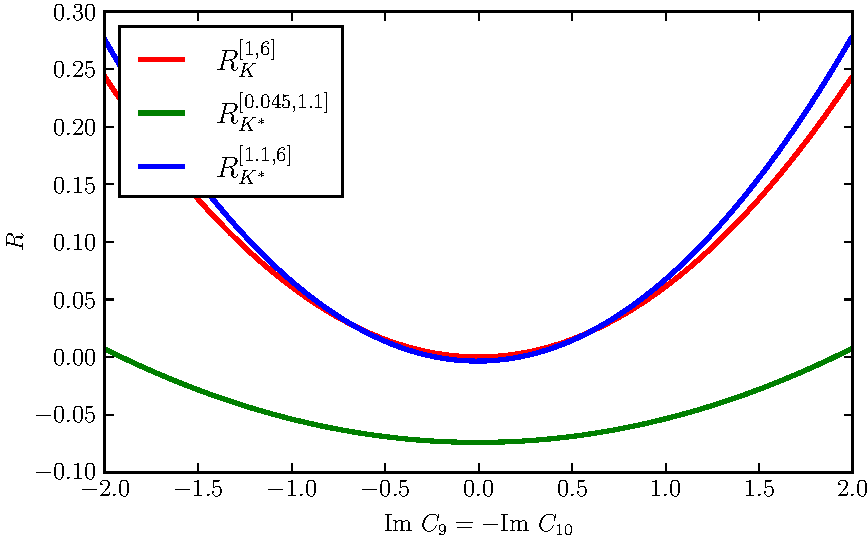
\includegraphics[width = 0.6\textwidth]{Figures/RK_im}
\caption{Values of $R_K$ and $R_{K^*}$ whith imaginary Wilson coefficients.}
\label{im:RK_im}
\end{figure}

 Figure \ref{im:RK_im} shows the values of the ratios $R_K$ and $R_{K^*}$ in their respective $q^2$ ranges, when both Wilson coefficients $C_9$ and $C_{10}$ are imaginary, and also we assume $C_9 = -C_{10}$. In all cases the minimum value for the ratio is attained at the SM point $C_9 = -C_{10} =0$. The addition of non-zero imaginary Wilson coefficients results in larger values of $R_K$ and $R_{K^*}$, at odds with the experimental values $R_{K^{(*)}}^{\mathrm{exp}} < R_{K^{(*)}}^{\mathrm{SM}}$.

\begin{figure}[H]
\centering
\resizebox{0.6\textwidth}{!}{%% Creator: Matplotlib, PGF backend
%%
%% To include the figure in your LaTeX document, write
%%   \input{<filename>.pgf}
%%
%% Make sure the required packages are loaded in your preamble
%%   \usepackage{pgf}
%%
%% Figures using additional raster images can only be included by \input if
%% they are in the same directory as the main LaTeX file. For loading figures
%% from other directories you can use the `import` package
%%   \usepackage{import}
%% and then include the figures with
%%   \import{<path to file>}{<filename>.pgf}
%%
%% Matplotlib used the following preamble
%%   \usepackage[utf8x]{inputenc}
%%   \usepackage[T1]{fontenc}
%%
\begingroup%
\makeatletter%
\begin{pgfpicture}%
\pgfpathrectangle{\pgfpointorigin}{\pgfqpoint{5.788530in}{3.577508in}}%
\pgfusepath{use as bounding box, clip}%
\begin{pgfscope}%
\pgfsetbuttcap%
\pgfsetmiterjoin%
\definecolor{currentfill}{rgb}{1.000000,1.000000,1.000000}%
\pgfsetfillcolor{currentfill}%
\pgfsetlinewidth{0.000000pt}%
\definecolor{currentstroke}{rgb}{1.000000,1.000000,1.000000}%
\pgfsetstrokecolor{currentstroke}%
\pgfsetdash{}{0pt}%
\pgfpathmoveto{\pgfqpoint{0.000000in}{0.000000in}}%
\pgfpathlineto{\pgfqpoint{5.788530in}{0.000000in}}%
\pgfpathlineto{\pgfqpoint{5.788530in}{3.577508in}}%
\pgfpathlineto{\pgfqpoint{0.000000in}{3.577508in}}%
\pgfpathclose%
\pgfusepath{fill}%
\end{pgfscope}%
\begin{pgfscope}%
\pgfsetbuttcap%
\pgfsetmiterjoin%
\definecolor{currentfill}{rgb}{1.000000,1.000000,1.000000}%
\pgfsetfillcolor{currentfill}%
\pgfsetlinewidth{0.000000pt}%
\definecolor{currentstroke}{rgb}{0.000000,0.000000,0.000000}%
\pgfsetstrokecolor{currentstroke}%
\pgfsetstrokeopacity{0.000000}%
\pgfsetdash{}{0pt}%
\pgfpathmoveto{\pgfqpoint{1.348313in}{0.424277in}}%
\pgfpathlineto{\pgfqpoint{4.440217in}{0.424277in}}%
\pgfpathlineto{\pgfqpoint{4.440217in}{3.516181in}}%
\pgfpathlineto{\pgfqpoint{1.348313in}{3.516181in}}%
\pgfpathclose%
\pgfusepath{fill}%
\end{pgfscope}%
\begin{pgfscope}%
\pgfpathrectangle{\pgfqpoint{1.348313in}{0.424277in}}{\pgfqpoint{3.091903in}{3.091903in}} %
\pgfusepath{clip}%
\pgfsetbuttcap%
\pgfsetroundjoin%
\definecolor{currentfill}{rgb}{0.984300,0.705900,0.682400}%
\pgfsetfillcolor{currentfill}%
\pgfsetlinewidth{0.000000pt}%
\definecolor{currentstroke}{rgb}{0.000000,0.000000,0.000000}%
\pgfsetstrokecolor{currentstroke}%
\pgfsetdash{}{0pt}%
\pgfpathmoveto{\pgfqpoint{2.254022in}{1.136163in}}%
\pgfpathlineto{\pgfqpoint{2.285254in}{1.129592in}}%
\pgfpathlineto{\pgfqpoint{2.316485in}{1.125148in}}%
\pgfpathlineto{\pgfqpoint{2.347716in}{1.122821in}}%
\pgfpathlineto{\pgfqpoint{2.378948in}{1.122582in}}%
\pgfpathlineto{\pgfqpoint{2.410179in}{1.124388in}}%
\pgfpathlineto{\pgfqpoint{2.441410in}{1.128038in}}%
\pgfpathlineto{\pgfqpoint{2.472642in}{1.133379in}}%
\pgfpathlineto{\pgfqpoint{2.503873in}{1.140339in}}%
\pgfpathlineto{\pgfqpoint{2.512096in}{1.142598in}}%
\pgfpathlineto{\pgfqpoint{2.535105in}{1.149353in}}%
\pgfpathlineto{\pgfqpoint{2.566336in}{1.160090in}}%
\pgfpathlineto{\pgfqpoint{2.597567in}{1.172165in}}%
\pgfpathlineto{\pgfqpoint{2.601449in}{1.173830in}}%
\pgfpathlineto{\pgfqpoint{2.628799in}{1.186192in}}%
\pgfpathlineto{\pgfqpoint{2.660030in}{1.201370in}}%
\pgfpathlineto{\pgfqpoint{2.667077in}{1.205061in}}%
\pgfpathlineto{\pgfqpoint{2.691261in}{1.218347in}}%
\pgfpathlineto{\pgfqpoint{2.722347in}{1.236292in}}%
\pgfpathlineto{\pgfqpoint{2.722493in}{1.236381in}}%
\pgfpathlineto{\pgfqpoint{2.753724in}{1.256360in}}%
\pgfpathlineto{\pgfqpoint{2.770668in}{1.267524in}}%
\pgfpathlineto{\pgfqpoint{2.784955in}{1.277355in}}%
\pgfpathlineto{\pgfqpoint{2.815320in}{1.298755in}}%
\pgfpathlineto{\pgfqpoint{2.816187in}{1.299392in}}%
\pgfpathlineto{\pgfqpoint{2.847418in}{1.323030in}}%
\pgfpathlineto{\pgfqpoint{2.856449in}{1.329986in}}%
\pgfpathlineto{\pgfqpoint{2.878649in}{1.347580in}}%
\pgfpathlineto{\pgfqpoint{2.895643in}{1.361218in}}%
\pgfpathlineto{\pgfqpoint{2.909881in}{1.372922in}}%
\pgfpathlineto{\pgfqpoint{2.933482in}{1.392449in}}%
\pgfpathlineto{\pgfqpoint{2.941112in}{1.398906in}}%
\pgfpathlineto{\pgfqpoint{2.970290in}{1.423680in}}%
\pgfpathlineto{\pgfqpoint{2.972343in}{1.425461in}}%
\pgfpathlineto{\pgfqpoint{3.003575in}{1.452665in}}%
\pgfpathlineto{\pgfqpoint{3.006148in}{1.454912in}}%
\pgfpathlineto{\pgfqpoint{3.034806in}{1.480388in}}%
\pgfpathlineto{\pgfqpoint{3.041296in}{1.486143in}}%
\pgfpathlineto{\pgfqpoint{3.066037in}{1.508330in}}%
\pgfpathlineto{\pgfqpoint{3.076167in}{1.517375in}}%
\pgfpathlineto{\pgfqpoint{3.097269in}{1.536349in}}%
\pgfpathlineto{\pgfqpoint{3.110977in}{1.548606in}}%
\pgfpathlineto{\pgfqpoint{3.128500in}{1.564374in}}%
\pgfpathlineto{\pgfqpoint{3.145800in}{1.579837in}}%
\pgfpathlineto{\pgfqpoint{3.159731in}{1.592364in}}%
\pgfpathlineto{\pgfqpoint{3.180694in}{1.611069in}}%
\pgfpathlineto{\pgfqpoint{3.190963in}{1.620283in}}%
\pgfpathlineto{\pgfqpoint{3.215706in}{1.642300in}}%
\pgfpathlineto{\pgfqpoint{3.222194in}{1.648093in}}%
\pgfpathlineto{\pgfqpoint{3.250871in}{1.673531in}}%
\pgfpathlineto{\pgfqpoint{3.253425in}{1.675800in}}%
\pgfpathlineto{\pgfqpoint{3.284657in}{1.703468in}}%
\pgfpathlineto{\pgfqpoint{3.286119in}{1.704763in}}%
\pgfpathlineto{\pgfqpoint{3.315888in}{1.731177in}}%
\pgfpathlineto{\pgfqpoint{3.321339in}{1.735994in}}%
\pgfpathlineto{\pgfqpoint{3.347120in}{1.758853in}}%
\pgfpathlineto{\pgfqpoint{3.356593in}{1.767225in}}%
\pgfpathlineto{\pgfqpoint{3.378351in}{1.786540in}}%
\pgfpathlineto{\pgfqpoint{3.391769in}{1.798457in}}%
\pgfpathlineto{\pgfqpoint{3.409582in}{1.814369in}}%
\pgfpathlineto{\pgfqpoint{3.426621in}{1.829688in}}%
\pgfpathlineto{\pgfqpoint{3.440814in}{1.842545in}}%
\pgfpathlineto{\pgfqpoint{3.460931in}{1.860919in}}%
\pgfpathlineto{\pgfqpoint{3.472045in}{1.871171in}}%
\pgfpathlineto{\pgfqpoint{3.494562in}{1.892151in}}%
\pgfpathlineto{\pgfqpoint{3.503276in}{1.900371in}}%
\pgfpathlineto{\pgfqpoint{3.527378in}{1.923382in}}%
\pgfpathlineto{\pgfqpoint{3.534508in}{1.930293in}}%
\pgfpathlineto{\pgfqpoint{3.559191in}{1.954613in}}%
\pgfpathlineto{\pgfqpoint{3.565739in}{1.961186in}}%
\pgfpathlineto{\pgfqpoint{3.589666in}{1.985845in}}%
\pgfpathlineto{\pgfqpoint{3.596970in}{1.993565in}}%
\pgfpathlineto{\pgfqpoint{3.618581in}{2.017076in}}%
\pgfpathlineto{\pgfqpoint{3.628202in}{2.027864in}}%
\pgfpathlineto{\pgfqpoint{3.645879in}{2.048307in}}%
\pgfpathlineto{\pgfqpoint{3.659433in}{2.064541in}}%
\pgfpathlineto{\pgfqpoint{3.671551in}{2.079539in}}%
\pgfpathlineto{\pgfqpoint{3.690664in}{2.104173in}}%
\pgfpathlineto{\pgfqpoint{3.695604in}{2.110770in}}%
\pgfpathlineto{\pgfqpoint{3.717809in}{2.142001in}}%
\pgfpathlineto{\pgfqpoint{3.721896in}{2.148142in}}%
\pgfpathlineto{\pgfqpoint{3.737823in}{2.173233in}}%
\pgfpathlineto{\pgfqpoint{3.753127in}{2.199174in}}%
\pgfpathlineto{\pgfqpoint{3.756098in}{2.204464in}}%
\pgfpathlineto{\pgfqpoint{3.771979in}{2.235695in}}%
\pgfpathlineto{\pgfqpoint{3.784358in}{2.262693in}}%
\pgfpathlineto{\pgfqpoint{3.786200in}{2.266927in}}%
\pgfpathlineto{\pgfqpoint{3.798008in}{2.298158in}}%
\pgfpathlineto{\pgfqpoint{3.807950in}{2.329390in}}%
\pgfpathlineto{\pgfqpoint{3.815590in}{2.359773in}}%
\pgfpathlineto{\pgfqpoint{3.815791in}{2.360621in}}%
\pgfpathlineto{\pgfqpoint{3.821064in}{2.391852in}}%
\pgfpathlineto{\pgfqpoint{3.824204in}{2.423084in}}%
\pgfpathlineto{\pgfqpoint{3.825155in}{2.454315in}}%
\pgfpathlineto{\pgfqpoint{3.823760in}{2.485546in}}%
\pgfpathlineto{\pgfqpoint{3.819806in}{2.516778in}}%
\pgfpathlineto{\pgfqpoint{3.815590in}{2.536983in}}%
\pgfpathlineto{\pgfqpoint{3.813096in}{2.548009in}}%
\pgfpathlineto{\pgfqpoint{3.803262in}{2.579240in}}%
\pgfpathlineto{\pgfqpoint{3.790676in}{2.610472in}}%
\pgfpathlineto{\pgfqpoint{3.784358in}{2.623295in}}%
\pgfpathlineto{\pgfqpoint{3.774454in}{2.641703in}}%
\pgfpathlineto{\pgfqpoint{3.754322in}{2.672934in}}%
\pgfpathlineto{\pgfqpoint{3.753127in}{2.674526in}}%
\pgfpathlineto{\pgfqpoint{3.728593in}{2.704166in}}%
\pgfpathlineto{\pgfqpoint{3.721896in}{2.711272in}}%
\pgfpathlineto{\pgfqpoint{3.696572in}{2.735397in}}%
\pgfpathlineto{\pgfqpoint{3.690664in}{2.740424in}}%
\pgfpathlineto{\pgfqpoint{3.659433in}{2.764160in}}%
\pgfpathlineto{\pgfqpoint{3.655740in}{2.766628in}}%
\pgfpathlineto{\pgfqpoint{3.628202in}{2.783255in}}%
\pgfpathlineto{\pgfqpoint{3.600108in}{2.797860in}}%
\pgfpathlineto{\pgfqpoint{3.596970in}{2.799336in}}%
\pgfpathlineto{\pgfqpoint{3.565739in}{2.811610in}}%
\pgfpathlineto{\pgfqpoint{3.534508in}{2.821451in}}%
\pgfpathlineto{\pgfqpoint{3.503276in}{2.829042in}}%
\pgfpathlineto{\pgfqpoint{3.502991in}{2.829091in}}%
\pgfpathlineto{\pgfqpoint{3.472045in}{2.833981in}}%
\pgfpathlineto{\pgfqpoint{3.440814in}{2.836913in}}%
\pgfpathlineto{\pgfqpoint{3.409582in}{2.837852in}}%
\pgfpathlineto{\pgfqpoint{3.378351in}{2.836822in}}%
\pgfpathlineto{\pgfqpoint{3.347120in}{2.833997in}}%
\pgfpathlineto{\pgfqpoint{3.315888in}{2.829508in}}%
\pgfpathlineto{\pgfqpoint{3.313773in}{2.829091in}}%
\pgfpathlineto{\pgfqpoint{3.284657in}{2.822943in}}%
\pgfpathlineto{\pgfqpoint{3.253425in}{2.814696in}}%
\pgfpathlineto{\pgfqpoint{3.222194in}{2.804889in}}%
\pgfpathlineto{\pgfqpoint{3.202682in}{2.797860in}}%
\pgfpathlineto{\pgfqpoint{3.190963in}{2.793362in}}%
\pgfpathlineto{\pgfqpoint{3.159731in}{2.780029in}}%
\pgfpathlineto{\pgfqpoint{3.130802in}{2.766628in}}%
\pgfpathlineto{\pgfqpoint{3.128500in}{2.765504in}}%
\pgfpathlineto{\pgfqpoint{3.097269in}{2.748961in}}%
\pgfpathlineto{\pgfqpoint{3.073089in}{2.735397in}}%
\pgfpathlineto{\pgfqpoint{3.066037in}{2.731247in}}%
\pgfpathlineto{\pgfqpoint{3.034806in}{2.711823in}}%
\pgfpathlineto{\pgfqpoint{3.022972in}{2.704166in}}%
\pgfpathlineto{\pgfqpoint{3.003575in}{2.691049in}}%
\pgfpathlineto{\pgfqpoint{2.977542in}{2.672934in}}%
\pgfpathlineto{\pgfqpoint{2.972343in}{2.669157in}}%
\pgfpathlineto{\pgfqpoint{2.941112in}{2.645791in}}%
\pgfpathlineto{\pgfqpoint{2.935787in}{2.641703in}}%
\pgfpathlineto{\pgfqpoint{2.909881in}{2.621035in}}%
\pgfpathlineto{\pgfqpoint{2.896853in}{2.610472in}}%
\pgfpathlineto{\pgfqpoint{2.878649in}{2.595289in}}%
\pgfpathlineto{\pgfqpoint{2.859591in}{2.579240in}}%
\pgfpathlineto{\pgfqpoint{2.847418in}{2.568740in}}%
\pgfpathlineto{\pgfqpoint{2.823532in}{2.548009in}}%
\pgfpathlineto{\pgfqpoint{2.816187in}{2.541488in}}%
\pgfpathlineto{\pgfqpoint{2.788450in}{2.516778in}}%
\pgfpathlineto{\pgfqpoint{2.784955in}{2.513597in}}%
\pgfpathlineto{\pgfqpoint{2.754161in}{2.485546in}}%
\pgfpathlineto{\pgfqpoint{2.753724in}{2.485140in}}%
\pgfpathlineto{\pgfqpoint{2.722493in}{2.456079in}}%
\pgfpathlineto{\pgfqpoint{2.720593in}{2.454315in}}%
\pgfpathlineto{\pgfqpoint{2.691261in}{2.426765in}}%
\pgfpathlineto{\pgfqpoint{2.687326in}{2.423084in}}%
\pgfpathlineto{\pgfqpoint{2.660030in}{2.397372in}}%
\pgfpathlineto{\pgfqpoint{2.654138in}{2.391852in}}%
\pgfpathlineto{\pgfqpoint{2.628799in}{2.367961in}}%
\pgfpathlineto{\pgfqpoint{2.620963in}{2.360621in}}%
\pgfpathlineto{\pgfqpoint{2.597567in}{2.338576in}}%
\pgfpathlineto{\pgfqpoint{2.587744in}{2.329390in}}%
\pgfpathlineto{\pgfqpoint{2.566336in}{2.309256in}}%
\pgfpathlineto{\pgfqpoint{2.554460in}{2.298158in}}%
\pgfpathlineto{\pgfqpoint{2.535105in}{2.280008in}}%
\pgfpathlineto{\pgfqpoint{2.521083in}{2.266927in}}%
\pgfpathlineto{\pgfqpoint{2.503873in}{2.250853in}}%
\pgfpathlineto{\pgfqpoint{2.487563in}{2.235695in}}%
\pgfpathlineto{\pgfqpoint{2.472642in}{2.221801in}}%
\pgfpathlineto{\pgfqpoint{2.453936in}{2.204464in}}%
\pgfpathlineto{\pgfqpoint{2.441410in}{2.192821in}}%
\pgfpathlineto{\pgfqpoint{2.420251in}{2.173233in}}%
\pgfpathlineto{\pgfqpoint{2.410179in}{2.163871in}}%
\pgfpathlineto{\pgfqpoint{2.386635in}{2.142001in}}%
\pgfpathlineto{\pgfqpoint{2.378948in}{2.134823in}}%
\pgfpathlineto{\pgfqpoint{2.353322in}{2.110770in}}%
\pgfpathlineto{\pgfqpoint{2.347716in}{2.105473in}}%
\pgfpathlineto{\pgfqpoint{2.320460in}{2.079539in}}%
\pgfpathlineto{\pgfqpoint{2.316485in}{2.075722in}}%
\pgfpathlineto{\pgfqpoint{2.288178in}{2.048307in}}%
\pgfpathlineto{\pgfqpoint{2.285254in}{2.045443in}}%
\pgfpathlineto{\pgfqpoint{2.256602in}{2.017076in}}%
\pgfpathlineto{\pgfqpoint{2.254022in}{2.014485in}}%
\pgfpathlineto{\pgfqpoint{2.225924in}{1.985845in}}%
\pgfpathlineto{\pgfqpoint{2.222791in}{1.982594in}}%
\pgfpathlineto{\pgfqpoint{2.196480in}{1.954613in}}%
\pgfpathlineto{\pgfqpoint{2.191560in}{1.949251in}}%
\pgfpathlineto{\pgfqpoint{2.168462in}{1.923382in}}%
\pgfpathlineto{\pgfqpoint{2.160328in}{1.914001in}}%
\pgfpathlineto{\pgfqpoint{2.141932in}{1.892151in}}%
\pgfpathlineto{\pgfqpoint{2.129097in}{1.876374in}}%
\pgfpathlineto{\pgfqpoint{2.116911in}{1.860919in}}%
\pgfpathlineto{\pgfqpoint{2.097866in}{1.835783in}}%
\pgfpathlineto{\pgfqpoint{2.093403in}{1.829688in}}%
\pgfpathlineto{\pgfqpoint{2.071708in}{1.798457in}}%
\pgfpathlineto{\pgfqpoint{2.066634in}{1.790657in}}%
\pgfpathlineto{\pgfqpoint{2.052078in}{1.767225in}}%
\pgfpathlineto{\pgfqpoint{2.035403in}{1.738346in}}%
\pgfpathlineto{\pgfqpoint{2.034109in}{1.735994in}}%
\pgfpathlineto{\pgfqpoint{2.018610in}{1.704763in}}%
\pgfpathlineto{\pgfqpoint{2.004627in}{1.673531in}}%
\pgfpathlineto{\pgfqpoint{2.004172in}{1.672359in}}%
\pgfpathlineto{\pgfqpoint{1.993127in}{1.642300in}}%
\pgfpathlineto{\pgfqpoint{1.983526in}{1.611069in}}%
\pgfpathlineto{\pgfqpoint{1.976023in}{1.579837in}}%
\pgfpathlineto{\pgfqpoint{1.972940in}{1.561565in}}%
\pgfpathlineto{\pgfqpoint{1.970885in}{1.548606in}}%
\pgfpathlineto{\pgfqpoint{1.968114in}{1.517375in}}%
\pgfpathlineto{\pgfqpoint{1.967562in}{1.486143in}}%
\pgfpathlineto{\pgfqpoint{1.969397in}{1.454912in}}%
\pgfpathlineto{\pgfqpoint{1.972940in}{1.430010in}}%
\pgfpathlineto{\pgfqpoint{1.973919in}{1.423680in}}%
\pgfpathlineto{\pgfqpoint{1.981588in}{1.392449in}}%
\pgfpathlineto{\pgfqpoint{1.992120in}{1.361218in}}%
\pgfpathlineto{\pgfqpoint{2.004172in}{1.333060in}}%
\pgfpathlineto{\pgfqpoint{2.005614in}{1.329986in}}%
\pgfpathlineto{\pgfqpoint{2.023430in}{1.298755in}}%
\pgfpathlineto{\pgfqpoint{2.035403in}{1.281183in}}%
\pgfpathlineto{\pgfqpoint{2.045713in}{1.267524in}}%
\pgfpathlineto{\pgfqpoint{2.066634in}{1.243661in}}%
\pgfpathlineto{\pgfqpoint{2.073871in}{1.236292in}}%
\pgfpathlineto{\pgfqpoint{2.097866in}{1.214806in}}%
\pgfpathlineto{\pgfqpoint{2.110125in}{1.205061in}}%
\pgfpathlineto{\pgfqpoint{2.129097in}{1.191581in}}%
\pgfpathlineto{\pgfqpoint{2.157723in}{1.173830in}}%
\pgfpathlineto{\pgfqpoint{2.160328in}{1.172369in}}%
\pgfpathlineto{\pgfqpoint{2.191560in}{1.157447in}}%
\pgfpathlineto{\pgfqpoint{2.222791in}{1.145157in}}%
\pgfpathlineto{\pgfqpoint{2.231062in}{1.142598in}}%
\pgfpathclose%
\pgfusepath{fill}%
\end{pgfscope}%
\begin{pgfscope}%
\pgfpathrectangle{\pgfqpoint{1.348313in}{0.424277in}}{\pgfqpoint{3.091903in}{3.091903in}} %
\pgfusepath{clip}%
\pgfsetbuttcap%
\pgfsetroundjoin%
\definecolor{currentfill}{rgb}{0.984300,0.705900,0.682400}%
\pgfsetfillcolor{currentfill}%
\pgfsetfillopacity{0.500000}%
\pgfsetlinewidth{0.000000pt}%
\definecolor{currentstroke}{rgb}{0.000000,0.000000,0.000000}%
\pgfsetstrokecolor{currentstroke}%
\pgfsetdash{}{0pt}%
\pgfpathmoveto{\pgfqpoint{2.160328in}{0.857434in}}%
\pgfpathlineto{\pgfqpoint{2.191560in}{0.849869in}}%
\pgfpathlineto{\pgfqpoint{2.222791in}{0.843622in}}%
\pgfpathlineto{\pgfqpoint{2.254022in}{0.838717in}}%
\pgfpathlineto{\pgfqpoint{2.285254in}{0.835076in}}%
\pgfpathlineto{\pgfqpoint{2.316485in}{0.832691in}}%
\pgfpathlineto{\pgfqpoint{2.347716in}{0.831576in}}%
\pgfpathlineto{\pgfqpoint{2.378948in}{0.831743in}}%
\pgfpathlineto{\pgfqpoint{2.410179in}{0.833195in}}%
\pgfpathlineto{\pgfqpoint{2.441410in}{0.835854in}}%
\pgfpathlineto{\pgfqpoint{2.472642in}{0.839665in}}%
\pgfpathlineto{\pgfqpoint{2.503873in}{0.844617in}}%
\pgfpathlineto{\pgfqpoint{2.535105in}{0.850694in}}%
\pgfpathlineto{\pgfqpoint{2.566336in}{0.857873in}}%
\pgfpathlineto{\pgfqpoint{2.580170in}{0.861516in}}%
\pgfpathlineto{\pgfqpoint{2.597567in}{0.866348in}}%
\pgfpathlineto{\pgfqpoint{2.628799in}{0.876018in}}%
\pgfpathlineto{\pgfqpoint{2.660030in}{0.886628in}}%
\pgfpathlineto{\pgfqpoint{2.676581in}{0.892748in}}%
\pgfpathlineto{\pgfqpoint{2.691261in}{0.898458in}}%
\pgfpathlineto{\pgfqpoint{2.722493in}{0.911541in}}%
\pgfpathlineto{\pgfqpoint{2.750434in}{0.923979in}}%
\pgfpathlineto{\pgfqpoint{2.753724in}{0.925519in}}%
\pgfpathlineto{\pgfqpoint{2.784955in}{0.940967in}}%
\pgfpathlineto{\pgfqpoint{2.812576in}{0.955210in}}%
\pgfpathlineto{\pgfqpoint{2.816187in}{0.957166in}}%
\pgfpathlineto{\pgfqpoint{2.847418in}{0.974848in}}%
\pgfpathlineto{\pgfqpoint{2.867221in}{0.986442in}}%
\pgfpathlineto{\pgfqpoint{2.878649in}{0.993426in}}%
\pgfpathlineto{\pgfqpoint{2.909881in}{1.013118in}}%
\pgfpathlineto{\pgfqpoint{2.916909in}{1.017673in}}%
\pgfpathlineto{\pgfqpoint{2.941112in}{1.033832in}}%
\pgfpathlineto{\pgfqpoint{2.963274in}{1.048904in}}%
\pgfpathlineto{\pgfqpoint{2.972343in}{1.055250in}}%
\pgfpathlineto{\pgfqpoint{3.003575in}{1.077498in}}%
\pgfpathlineto{\pgfqpoint{3.007206in}{1.080136in}}%
\pgfpathlineto{\pgfqpoint{3.034806in}{1.100714in}}%
\pgfpathlineto{\pgfqpoint{3.048934in}{1.111367in}}%
\pgfpathlineto{\pgfqpoint{3.066037in}{1.124599in}}%
\pgfpathlineto{\pgfqpoint{3.089121in}{1.142598in}}%
\pgfpathlineto{\pgfqpoint{3.097269in}{1.149105in}}%
\pgfpathlineto{\pgfqpoint{3.128057in}{1.173830in}}%
\pgfpathlineto{\pgfqpoint{3.128500in}{1.174192in}}%
\pgfpathlineto{\pgfqpoint{3.159731in}{1.199953in}}%
\pgfpathlineto{\pgfqpoint{3.165904in}{1.205061in}}%
\pgfpathlineto{\pgfqpoint{3.190963in}{1.226120in}}%
\pgfpathlineto{\pgfqpoint{3.203051in}{1.236292in}}%
\pgfpathlineto{\pgfqpoint{3.222194in}{1.252641in}}%
\pgfpathlineto{\pgfqpoint{3.239614in}{1.267524in}}%
\pgfpathlineto{\pgfqpoint{3.253425in}{1.279492in}}%
\pgfpathlineto{\pgfqpoint{3.275664in}{1.298755in}}%
\pgfpathlineto{\pgfqpoint{3.284657in}{1.306650in}}%
\pgfpathlineto{\pgfqpoint{3.311278in}{1.329986in}}%
\pgfpathlineto{\pgfqpoint{3.315888in}{1.334061in}}%
\pgfpathlineto{\pgfqpoint{3.346685in}{1.361218in}}%
\pgfpathlineto{\pgfqpoint{3.347120in}{1.361603in}}%
\pgfpathlineto{\pgfqpoint{3.378351in}{1.389335in}}%
\pgfpathlineto{\pgfqpoint{3.381864in}{1.392449in}}%
\pgfpathlineto{\pgfqpoint{3.409582in}{1.417168in}}%
\pgfpathlineto{\pgfqpoint{3.416890in}{1.423680in}}%
\pgfpathlineto{\pgfqpoint{3.440814in}{1.445134in}}%
\pgfpathlineto{\pgfqpoint{3.451728in}{1.454912in}}%
\pgfpathlineto{\pgfqpoint{3.472045in}{1.473234in}}%
\pgfpathlineto{\pgfqpoint{3.486375in}{1.486143in}}%
\pgfpathlineto{\pgfqpoint{3.503276in}{1.501439in}}%
\pgfpathlineto{\pgfqpoint{3.520901in}{1.517375in}}%
\pgfpathlineto{\pgfqpoint{3.534508in}{1.529724in}}%
\pgfpathlineto{\pgfqpoint{3.555302in}{1.548606in}}%
\pgfpathlineto{\pgfqpoint{3.565739in}{1.558126in}}%
\pgfpathlineto{\pgfqpoint{3.589423in}{1.579837in}}%
\pgfpathlineto{\pgfqpoint{3.596970in}{1.586795in}}%
\pgfpathlineto{\pgfqpoint{3.623149in}{1.611069in}}%
\pgfpathlineto{\pgfqpoint{3.628202in}{1.615784in}}%
\pgfpathlineto{\pgfqpoint{3.656423in}{1.642300in}}%
\pgfpathlineto{\pgfqpoint{3.659433in}{1.645148in}}%
\pgfpathlineto{\pgfqpoint{3.689202in}{1.673531in}}%
\pgfpathlineto{\pgfqpoint{3.690664in}{1.674937in}}%
\pgfpathlineto{\pgfqpoint{3.721422in}{1.704763in}}%
\pgfpathlineto{\pgfqpoint{3.721896in}{1.705226in}}%
\pgfpathlineto{\pgfqpoint{3.752876in}{1.735994in}}%
\pgfpathlineto{\pgfqpoint{3.753127in}{1.736246in}}%
\pgfpathlineto{\pgfqpoint{3.783468in}{1.767225in}}%
\pgfpathlineto{\pgfqpoint{3.784358in}{1.768147in}}%
\pgfpathlineto{\pgfqpoint{3.813142in}{1.798457in}}%
\pgfpathlineto{\pgfqpoint{3.815590in}{1.801075in}}%
\pgfpathlineto{\pgfqpoint{3.841841in}{1.829688in}}%
\pgfpathlineto{\pgfqpoint{3.846821in}{1.835221in}}%
\pgfpathlineto{\pgfqpoint{3.869488in}{1.860919in}}%
\pgfpathlineto{\pgfqpoint{3.878052in}{1.870845in}}%
\pgfpathlineto{\pgfqpoint{3.895868in}{1.892151in}}%
\pgfpathlineto{\pgfqpoint{3.909284in}{1.908601in}}%
\pgfpathlineto{\pgfqpoint{3.920911in}{1.923382in}}%
\pgfpathlineto{\pgfqpoint{3.940515in}{1.949020in}}%
\pgfpathlineto{\pgfqpoint{3.944639in}{1.954613in}}%
\pgfpathlineto{\pgfqpoint{3.966856in}{1.985845in}}%
\pgfpathlineto{\pgfqpoint{3.971746in}{1.993009in}}%
\pgfpathlineto{\pgfqpoint{3.987551in}{2.017076in}}%
\pgfpathlineto{\pgfqpoint{4.002978in}{2.041628in}}%
\pgfpathlineto{\pgfqpoint{4.007014in}{2.048307in}}%
\pgfpathlineto{\pgfqpoint{4.024874in}{2.079539in}}%
\pgfpathlineto{\pgfqpoint{4.034209in}{2.096830in}}%
\pgfpathlineto{\pgfqpoint{4.041529in}{2.110770in}}%
\pgfpathlineto{\pgfqpoint{4.056857in}{2.142001in}}%
\pgfpathlineto{\pgfqpoint{4.065441in}{2.160952in}}%
\pgfpathlineto{\pgfqpoint{4.070900in}{2.173233in}}%
\pgfpathlineto{\pgfqpoint{4.083507in}{2.204464in}}%
\pgfpathlineto{\pgfqpoint{4.094839in}{2.235695in}}%
\pgfpathlineto{\pgfqpoint{4.096672in}{2.241431in}}%
\pgfpathlineto{\pgfqpoint{4.104631in}{2.266927in}}%
\pgfpathlineto{\pgfqpoint{4.113037in}{2.298158in}}%
\pgfpathlineto{\pgfqpoint{4.119986in}{2.329390in}}%
\pgfpathlineto{\pgfqpoint{4.125392in}{2.360621in}}%
\pgfpathlineto{\pgfqpoint{4.127903in}{2.381019in}}%
\pgfpathlineto{\pgfqpoint{4.129200in}{2.391852in}}%
\pgfpathlineto{\pgfqpoint{4.131409in}{2.423084in}}%
\pgfpathlineto{\pgfqpoint{4.132091in}{2.454315in}}%
\pgfpathlineto{\pgfqpoint{4.131188in}{2.485546in}}%
\pgfpathlineto{\pgfqpoint{4.128613in}{2.516778in}}%
\pgfpathlineto{\pgfqpoint{4.127903in}{2.522003in}}%
\pgfpathlineto{\pgfqpoint{4.124281in}{2.548009in}}%
\pgfpathlineto{\pgfqpoint{4.118260in}{2.579240in}}%
\pgfpathlineto{\pgfqpoint{4.110610in}{2.610472in}}%
\pgfpathlineto{\pgfqpoint{4.101334in}{2.641703in}}%
\pgfpathlineto{\pgfqpoint{4.096672in}{2.654885in}}%
\pgfpathlineto{\pgfqpoint{4.090132in}{2.672934in}}%
\pgfpathlineto{\pgfqpoint{4.077053in}{2.704166in}}%
\pgfpathlineto{\pgfqpoint{4.065441in}{2.728736in}}%
\pgfpathlineto{\pgfqpoint{4.062215in}{2.735397in}}%
\pgfpathlineto{\pgfqpoint{4.045357in}{2.766628in}}%
\pgfpathlineto{\pgfqpoint{4.034209in}{2.785453in}}%
\pgfpathlineto{\pgfqpoint{4.026578in}{2.797860in}}%
\pgfpathlineto{\pgfqpoint{4.005557in}{2.829091in}}%
\pgfpathlineto{\pgfqpoint{4.002978in}{2.832613in}}%
\pgfpathlineto{\pgfqpoint{3.981529in}{2.860322in}}%
\pgfpathlineto{\pgfqpoint{3.971746in}{2.872066in}}%
\pgfpathlineto{\pgfqpoint{3.954516in}{2.891554in}}%
\pgfpathlineto{\pgfqpoint{3.940515in}{2.906356in}}%
\pgfpathlineto{\pgfqpoint{3.923945in}{2.922785in}}%
\pgfpathlineto{\pgfqpoint{3.909284in}{2.936436in}}%
\pgfpathlineto{\pgfqpoint{3.889040in}{2.954016in}}%
\pgfpathlineto{\pgfqpoint{3.878052in}{2.962911in}}%
\pgfpathlineto{\pgfqpoint{3.848435in}{2.985248in}}%
\pgfpathlineto{\pgfqpoint{3.846821in}{2.986383in}}%
\pgfpathlineto{\pgfqpoint{3.815590in}{3.006886in}}%
\pgfpathlineto{\pgfqpoint{3.799902in}{3.016479in}}%
\pgfpathlineto{\pgfqpoint{3.784358in}{3.025385in}}%
\pgfpathlineto{\pgfqpoint{3.753127in}{3.041900in}}%
\pgfpathlineto{\pgfqpoint{3.741086in}{3.047711in}}%
\pgfpathlineto{\pgfqpoint{3.721896in}{3.056423in}}%
\pgfpathlineto{\pgfqpoint{3.690664in}{3.069239in}}%
\pgfpathlineto{\pgfqpoint{3.664370in}{3.078942in}}%
\pgfpathlineto{\pgfqpoint{3.659433in}{3.080662in}}%
\pgfpathlineto{\pgfqpoint{3.628202in}{3.090240in}}%
\pgfpathlineto{\pgfqpoint{3.596970in}{3.098539in}}%
\pgfpathlineto{\pgfqpoint{3.565739in}{3.105515in}}%
\pgfpathlineto{\pgfqpoint{3.539852in}{3.110173in}}%
\pgfpathlineto{\pgfqpoint{3.534508in}{3.111096in}}%
\pgfpathlineto{\pgfqpoint{3.503276in}{3.115250in}}%
\pgfpathlineto{\pgfqpoint{3.472045in}{3.118191in}}%
\pgfpathlineto{\pgfqpoint{3.440814in}{3.119900in}}%
\pgfpathlineto{\pgfqpoint{3.409582in}{3.120361in}}%
\pgfpathlineto{\pgfqpoint{3.378351in}{3.119567in}}%
\pgfpathlineto{\pgfqpoint{3.347120in}{3.117588in}}%
\pgfpathlineto{\pgfqpoint{3.315888in}{3.114469in}}%
\pgfpathlineto{\pgfqpoint{3.284657in}{3.110219in}}%
\pgfpathlineto{\pgfqpoint{3.284393in}{3.110173in}}%
\pgfpathlineto{\pgfqpoint{3.253425in}{3.104616in}}%
\pgfpathlineto{\pgfqpoint{3.222194in}{3.097864in}}%
\pgfpathlineto{\pgfqpoint{3.190963in}{3.090038in}}%
\pgfpathlineto{\pgfqpoint{3.159731in}{3.081227in}}%
\pgfpathlineto{\pgfqpoint{3.152448in}{3.078942in}}%
\pgfpathlineto{\pgfqpoint{3.128500in}{3.071031in}}%
\pgfpathlineto{\pgfqpoint{3.097269in}{3.059748in}}%
\pgfpathlineto{\pgfqpoint{3.066438in}{3.047711in}}%
\pgfpathlineto{\pgfqpoint{3.066037in}{3.047546in}}%
\pgfpathlineto{\pgfqpoint{3.034806in}{3.033749in}}%
\pgfpathlineto{\pgfqpoint{3.003575in}{3.019210in}}%
\pgfpathlineto{\pgfqpoint{2.998020in}{3.016479in}}%
\pgfpathlineto{\pgfqpoint{2.972343in}{3.003233in}}%
\pgfpathlineto{\pgfqpoint{2.941112in}{2.986454in}}%
\pgfpathlineto{\pgfqpoint{2.938966in}{2.985248in}}%
\pgfpathlineto{\pgfqpoint{2.909881in}{2.968108in}}%
\pgfpathlineto{\pgfqpoint{2.886698in}{2.954016in}}%
\pgfpathlineto{\pgfqpoint{2.878649in}{2.948910in}}%
\pgfpathlineto{\pgfqpoint{2.847418in}{2.928516in}}%
\pgfpathlineto{\pgfqpoint{2.838860in}{2.922785in}}%
\pgfpathlineto{\pgfqpoint{2.816187in}{2.907144in}}%
\pgfpathlineto{\pgfqpoint{2.793997in}{2.891554in}}%
\pgfpathlineto{\pgfqpoint{2.784955in}{2.885018in}}%
\pgfpathlineto{\pgfqpoint{2.753724in}{2.862056in}}%
\pgfpathlineto{\pgfqpoint{2.751410in}{2.860322in}}%
\pgfpathlineto{\pgfqpoint{2.722493in}{2.838074in}}%
\pgfpathlineto{\pgfqpoint{2.710934in}{2.829091in}}%
\pgfpathlineto{\pgfqpoint{2.691261in}{2.813407in}}%
\pgfpathlineto{\pgfqpoint{2.671907in}{2.797860in}}%
\pgfpathlineto{\pgfqpoint{2.660030in}{2.788088in}}%
\pgfpathlineto{\pgfqpoint{2.634090in}{2.766628in}}%
\pgfpathlineto{\pgfqpoint{2.628799in}{2.762172in}}%
\pgfpathlineto{\pgfqpoint{2.597567in}{2.735759in}}%
\pgfpathlineto{\pgfqpoint{2.597142in}{2.735397in}}%
\pgfpathlineto{\pgfqpoint{2.566336in}{2.708752in}}%
\pgfpathlineto{\pgfqpoint{2.561042in}{2.704166in}}%
\pgfpathlineto{\pgfqpoint{2.535105in}{2.681361in}}%
\pgfpathlineto{\pgfqpoint{2.525526in}{2.672934in}}%
\pgfpathlineto{\pgfqpoint{2.503873in}{2.653613in}}%
\pgfpathlineto{\pgfqpoint{2.490519in}{2.641703in}}%
\pgfpathlineto{\pgfqpoint{2.472642in}{2.625544in}}%
\pgfpathlineto{\pgfqpoint{2.455942in}{2.610472in}}%
\pgfpathlineto{\pgfqpoint{2.441410in}{2.597250in}}%
\pgfpathlineto{\pgfqpoint{2.421570in}{2.579240in}}%
\pgfpathlineto{\pgfqpoint{2.410179in}{2.568833in}}%
\pgfpathlineto{\pgfqpoint{2.387337in}{2.548009in}}%
\pgfpathlineto{\pgfqpoint{2.378948in}{2.540311in}}%
\pgfpathlineto{\pgfqpoint{2.353277in}{2.516778in}}%
\pgfpathlineto{\pgfqpoint{2.347716in}{2.511646in}}%
\pgfpathlineto{\pgfqpoint{2.319399in}{2.485546in}}%
\pgfpathlineto{\pgfqpoint{2.316485in}{2.482842in}}%
\pgfpathlineto{\pgfqpoint{2.285701in}{2.454315in}}%
\pgfpathlineto{\pgfqpoint{2.285254in}{2.453898in}}%
\pgfpathlineto{\pgfqpoint{2.254022in}{2.424807in}}%
\pgfpathlineto{\pgfqpoint{2.252172in}{2.423084in}}%
\pgfpathlineto{\pgfqpoint{2.222791in}{2.395609in}}%
\pgfpathlineto{\pgfqpoint{2.218789in}{2.391852in}}%
\pgfpathlineto{\pgfqpoint{2.191560in}{2.366178in}}%
\pgfpathlineto{\pgfqpoint{2.185693in}{2.360621in}}%
\pgfpathlineto{\pgfqpoint{2.160328in}{2.336462in}}%
\pgfpathlineto{\pgfqpoint{2.152940in}{2.329390in}}%
\pgfpathlineto{\pgfqpoint{2.129097in}{2.306413in}}%
\pgfpathlineto{\pgfqpoint{2.120580in}{2.298158in}}%
\pgfpathlineto{\pgfqpoint{2.097866in}{2.275983in}}%
\pgfpathlineto{\pgfqpoint{2.088655in}{2.266927in}}%
\pgfpathlineto{\pgfqpoint{2.066634in}{2.245104in}}%
\pgfpathlineto{\pgfqpoint{2.057255in}{2.235695in}}%
\pgfpathlineto{\pgfqpoint{2.035403in}{2.213565in}}%
\pgfpathlineto{\pgfqpoint{2.026541in}{2.204464in}}%
\pgfpathlineto{\pgfqpoint{2.004172in}{2.181225in}}%
\pgfpathlineto{\pgfqpoint{1.996593in}{2.173233in}}%
\pgfpathlineto{\pgfqpoint{1.972940in}{2.147950in}}%
\pgfpathlineto{\pgfqpoint{1.967464in}{2.142001in}}%
\pgfpathlineto{\pgfqpoint{1.941709in}{2.113573in}}%
\pgfpathlineto{\pgfqpoint{1.939214in}{2.110770in}}%
\pgfpathlineto{\pgfqpoint{1.911978in}{2.079539in}}%
\pgfpathlineto{\pgfqpoint{1.910478in}{2.077777in}}%
\pgfpathlineto{\pgfqpoint{1.886120in}{2.048307in}}%
\pgfpathlineto{\pgfqpoint{1.879246in}{2.039787in}}%
\pgfpathlineto{\pgfqpoint{1.861558in}{2.017076in}}%
\pgfpathlineto{\pgfqpoint{1.848015in}{1.999201in}}%
\pgfpathlineto{\pgfqpoint{1.838249in}{1.985845in}}%
\pgfpathlineto{\pgfqpoint{1.816784in}{1.955539in}}%
\pgfpathlineto{\pgfqpoint{1.816151in}{1.954613in}}%
\pgfpathlineto{\pgfqpoint{1.795764in}{1.923382in}}%
\pgfpathlineto{\pgfqpoint{1.785552in}{1.907039in}}%
\pgfpathlineto{\pgfqpoint{1.776598in}{1.892151in}}%
\pgfpathlineto{\pgfqpoint{1.758764in}{1.860919in}}%
\pgfpathlineto{\pgfqpoint{1.754321in}{1.852660in}}%
\pgfpathlineto{\pgfqpoint{1.742296in}{1.829688in}}%
\pgfpathlineto{\pgfqpoint{1.726968in}{1.798457in}}%
\pgfpathlineto{\pgfqpoint{1.723089in}{1.789876in}}%
\pgfpathlineto{\pgfqpoint{1.713037in}{1.767225in}}%
\pgfpathlineto{\pgfqpoint{1.700419in}{1.735994in}}%
\pgfpathlineto{\pgfqpoint{1.691858in}{1.712401in}}%
\pgfpathlineto{\pgfqpoint{1.689145in}{1.704763in}}%
\pgfpathlineto{\pgfqpoint{1.679392in}{1.673531in}}%
\pgfpathlineto{\pgfqpoint{1.670980in}{1.642300in}}%
\pgfpathlineto{\pgfqpoint{1.664031in}{1.611069in}}%
\pgfpathlineto{\pgfqpoint{1.660627in}{1.591352in}}%
\pgfpathlineto{\pgfqpoint{1.658692in}{1.579837in}}%
\pgfpathlineto{\pgfqpoint{1.654981in}{1.548606in}}%
\pgfpathlineto{\pgfqpoint{1.652815in}{1.517375in}}%
\pgfpathlineto{\pgfqpoint{1.652193in}{1.486143in}}%
\pgfpathlineto{\pgfqpoint{1.653177in}{1.454912in}}%
\pgfpathlineto{\pgfqpoint{1.655858in}{1.423680in}}%
\pgfpathlineto{\pgfqpoint{1.660215in}{1.392449in}}%
\pgfpathlineto{\pgfqpoint{1.660627in}{1.390319in}}%
\pgfpathlineto{\pgfqpoint{1.666392in}{1.361218in}}%
\pgfpathlineto{\pgfqpoint{1.674239in}{1.329986in}}%
\pgfpathlineto{\pgfqpoint{1.683744in}{1.298755in}}%
\pgfpathlineto{\pgfqpoint{1.691858in}{1.276301in}}%
\pgfpathlineto{\pgfqpoint{1.695112in}{1.267524in}}%
\pgfpathlineto{\pgfqpoint{1.708511in}{1.236292in}}%
\pgfpathlineto{\pgfqpoint{1.723089in}{1.206135in}}%
\pgfpathlineto{\pgfqpoint{1.723622in}{1.205061in}}%
\pgfpathlineto{\pgfqpoint{1.740905in}{1.173830in}}%
\pgfpathlineto{\pgfqpoint{1.754321in}{1.151707in}}%
\pgfpathlineto{\pgfqpoint{1.760065in}{1.142598in}}%
\pgfpathlineto{\pgfqpoint{1.781640in}{1.111367in}}%
\pgfpathlineto{\pgfqpoint{1.785552in}{1.106158in}}%
\pgfpathlineto{\pgfqpoint{1.806243in}{1.080136in}}%
\pgfpathlineto{\pgfqpoint{1.816784in}{1.067823in}}%
\pgfpathlineto{\pgfqpoint{1.834002in}{1.048904in}}%
\pgfpathlineto{\pgfqpoint{1.848015in}{1.034517in}}%
\pgfpathlineto{\pgfqpoint{1.865544in}{1.017673in}}%
\pgfpathlineto{\pgfqpoint{1.879246in}{1.005313in}}%
\pgfpathlineto{\pgfqpoint{1.901729in}{0.986442in}}%
\pgfpathlineto{\pgfqpoint{1.910478in}{0.979599in}}%
\pgfpathlineto{\pgfqpoint{1.941709in}{0.956920in}}%
\pgfpathlineto{\pgfqpoint{1.944237in}{0.955210in}}%
\pgfpathlineto{\pgfqpoint{1.972940in}{0.937125in}}%
\pgfpathlineto{\pgfqpoint{1.995399in}{0.923979in}}%
\pgfpathlineto{\pgfqpoint{2.004172in}{0.919168in}}%
\pgfpathlineto{\pgfqpoint{2.035403in}{0.903467in}}%
\pgfpathlineto{\pgfqpoint{2.058826in}{0.892748in}}%
\pgfpathlineto{\pgfqpoint{2.066634in}{0.889386in}}%
\pgfpathlineto{\pgfqpoint{2.097866in}{0.877348in}}%
\pgfpathlineto{\pgfqpoint{2.129097in}{0.866595in}}%
\pgfpathlineto{\pgfqpoint{2.145962in}{0.861516in}}%
\pgfpathclose%
\pgfpathmoveto{\pgfqpoint{2.231062in}{1.142598in}}%
\pgfpathlineto{\pgfqpoint{2.222791in}{1.145157in}}%
\pgfpathlineto{\pgfqpoint{2.191560in}{1.157447in}}%
\pgfpathlineto{\pgfqpoint{2.160328in}{1.172369in}}%
\pgfpathlineto{\pgfqpoint{2.157723in}{1.173830in}}%
\pgfpathlineto{\pgfqpoint{2.129097in}{1.191581in}}%
\pgfpathlineto{\pgfqpoint{2.110125in}{1.205061in}}%
\pgfpathlineto{\pgfqpoint{2.097866in}{1.214806in}}%
\pgfpathlineto{\pgfqpoint{2.073871in}{1.236292in}}%
\pgfpathlineto{\pgfqpoint{2.066634in}{1.243661in}}%
\pgfpathlineto{\pgfqpoint{2.045713in}{1.267524in}}%
\pgfpathlineto{\pgfqpoint{2.035403in}{1.281183in}}%
\pgfpathlineto{\pgfqpoint{2.023430in}{1.298755in}}%
\pgfpathlineto{\pgfqpoint{2.005614in}{1.329986in}}%
\pgfpathlineto{\pgfqpoint{2.004172in}{1.333060in}}%
\pgfpathlineto{\pgfqpoint{1.992120in}{1.361218in}}%
\pgfpathlineto{\pgfqpoint{1.981588in}{1.392449in}}%
\pgfpathlineto{\pgfqpoint{1.973919in}{1.423680in}}%
\pgfpathlineto{\pgfqpoint{1.972940in}{1.430010in}}%
\pgfpathlineto{\pgfqpoint{1.969397in}{1.454912in}}%
\pgfpathlineto{\pgfqpoint{1.967562in}{1.486143in}}%
\pgfpathlineto{\pgfqpoint{1.968114in}{1.517375in}}%
\pgfpathlineto{\pgfqpoint{1.970885in}{1.548606in}}%
\pgfpathlineto{\pgfqpoint{1.972940in}{1.561565in}}%
\pgfpathlineto{\pgfqpoint{1.976023in}{1.579837in}}%
\pgfpathlineto{\pgfqpoint{1.983526in}{1.611069in}}%
\pgfpathlineto{\pgfqpoint{1.993127in}{1.642300in}}%
\pgfpathlineto{\pgfqpoint{2.004172in}{1.672359in}}%
\pgfpathlineto{\pgfqpoint{2.004627in}{1.673531in}}%
\pgfpathlineto{\pgfqpoint{2.018610in}{1.704763in}}%
\pgfpathlineto{\pgfqpoint{2.034109in}{1.735994in}}%
\pgfpathlineto{\pgfqpoint{2.035403in}{1.738346in}}%
\pgfpathlineto{\pgfqpoint{2.052078in}{1.767225in}}%
\pgfpathlineto{\pgfqpoint{2.066634in}{1.790657in}}%
\pgfpathlineto{\pgfqpoint{2.071708in}{1.798457in}}%
\pgfpathlineto{\pgfqpoint{2.093403in}{1.829688in}}%
\pgfpathlineto{\pgfqpoint{2.097866in}{1.835783in}}%
\pgfpathlineto{\pgfqpoint{2.116911in}{1.860919in}}%
\pgfpathlineto{\pgfqpoint{2.129097in}{1.876374in}}%
\pgfpathlineto{\pgfqpoint{2.141932in}{1.892151in}}%
\pgfpathlineto{\pgfqpoint{2.160328in}{1.914001in}}%
\pgfpathlineto{\pgfqpoint{2.168462in}{1.923382in}}%
\pgfpathlineto{\pgfqpoint{2.191560in}{1.949251in}}%
\pgfpathlineto{\pgfqpoint{2.196480in}{1.954613in}}%
\pgfpathlineto{\pgfqpoint{2.222791in}{1.982594in}}%
\pgfpathlineto{\pgfqpoint{2.225924in}{1.985845in}}%
\pgfpathlineto{\pgfqpoint{2.254022in}{2.014485in}}%
\pgfpathlineto{\pgfqpoint{2.256602in}{2.017076in}}%
\pgfpathlineto{\pgfqpoint{2.285254in}{2.045443in}}%
\pgfpathlineto{\pgfqpoint{2.288178in}{2.048307in}}%
\pgfpathlineto{\pgfqpoint{2.316485in}{2.075722in}}%
\pgfpathlineto{\pgfqpoint{2.320460in}{2.079539in}}%
\pgfpathlineto{\pgfqpoint{2.347716in}{2.105473in}}%
\pgfpathlineto{\pgfqpoint{2.353322in}{2.110770in}}%
\pgfpathlineto{\pgfqpoint{2.378948in}{2.134823in}}%
\pgfpathlineto{\pgfqpoint{2.386635in}{2.142001in}}%
\pgfpathlineto{\pgfqpoint{2.410179in}{2.163871in}}%
\pgfpathlineto{\pgfqpoint{2.420251in}{2.173233in}}%
\pgfpathlineto{\pgfqpoint{2.441410in}{2.192821in}}%
\pgfpathlineto{\pgfqpoint{2.453936in}{2.204464in}}%
\pgfpathlineto{\pgfqpoint{2.472642in}{2.221801in}}%
\pgfpathlineto{\pgfqpoint{2.487563in}{2.235695in}}%
\pgfpathlineto{\pgfqpoint{2.503873in}{2.250853in}}%
\pgfpathlineto{\pgfqpoint{2.521083in}{2.266927in}}%
\pgfpathlineto{\pgfqpoint{2.535105in}{2.280008in}}%
\pgfpathlineto{\pgfqpoint{2.554460in}{2.298158in}}%
\pgfpathlineto{\pgfqpoint{2.566336in}{2.309256in}}%
\pgfpathlineto{\pgfqpoint{2.587744in}{2.329390in}}%
\pgfpathlineto{\pgfqpoint{2.597567in}{2.338576in}}%
\pgfpathlineto{\pgfqpoint{2.620963in}{2.360621in}}%
\pgfpathlineto{\pgfqpoint{2.628799in}{2.367961in}}%
\pgfpathlineto{\pgfqpoint{2.654138in}{2.391852in}}%
\pgfpathlineto{\pgfqpoint{2.660030in}{2.397372in}}%
\pgfpathlineto{\pgfqpoint{2.687326in}{2.423084in}}%
\pgfpathlineto{\pgfqpoint{2.691261in}{2.426765in}}%
\pgfpathlineto{\pgfqpoint{2.720593in}{2.454315in}}%
\pgfpathlineto{\pgfqpoint{2.722493in}{2.456079in}}%
\pgfpathlineto{\pgfqpoint{2.753724in}{2.485140in}}%
\pgfpathlineto{\pgfqpoint{2.754161in}{2.485546in}}%
\pgfpathlineto{\pgfqpoint{2.784955in}{2.513597in}}%
\pgfpathlineto{\pgfqpoint{2.788450in}{2.516778in}}%
\pgfpathlineto{\pgfqpoint{2.816187in}{2.541488in}}%
\pgfpathlineto{\pgfqpoint{2.823532in}{2.548009in}}%
\pgfpathlineto{\pgfqpoint{2.847418in}{2.568740in}}%
\pgfpathlineto{\pgfqpoint{2.859591in}{2.579240in}}%
\pgfpathlineto{\pgfqpoint{2.878649in}{2.595289in}}%
\pgfpathlineto{\pgfqpoint{2.896853in}{2.610472in}}%
\pgfpathlineto{\pgfqpoint{2.909881in}{2.621035in}}%
\pgfpathlineto{\pgfqpoint{2.935787in}{2.641703in}}%
\pgfpathlineto{\pgfqpoint{2.941112in}{2.645791in}}%
\pgfpathlineto{\pgfqpoint{2.972343in}{2.669157in}}%
\pgfpathlineto{\pgfqpoint{2.977542in}{2.672934in}}%
\pgfpathlineto{\pgfqpoint{3.003575in}{2.691049in}}%
\pgfpathlineto{\pgfqpoint{3.022972in}{2.704166in}}%
\pgfpathlineto{\pgfqpoint{3.034806in}{2.711823in}}%
\pgfpathlineto{\pgfqpoint{3.066037in}{2.731247in}}%
\pgfpathlineto{\pgfqpoint{3.073089in}{2.735397in}}%
\pgfpathlineto{\pgfqpoint{3.097269in}{2.748961in}}%
\pgfpathlineto{\pgfqpoint{3.128500in}{2.765504in}}%
\pgfpathlineto{\pgfqpoint{3.130802in}{2.766628in}}%
\pgfpathlineto{\pgfqpoint{3.159731in}{2.780029in}}%
\pgfpathlineto{\pgfqpoint{3.190963in}{2.793362in}}%
\pgfpathlineto{\pgfqpoint{3.202682in}{2.797860in}}%
\pgfpathlineto{\pgfqpoint{3.222194in}{2.804889in}}%
\pgfpathlineto{\pgfqpoint{3.253425in}{2.814696in}}%
\pgfpathlineto{\pgfqpoint{3.284657in}{2.822943in}}%
\pgfpathlineto{\pgfqpoint{3.313773in}{2.829091in}}%
\pgfpathlineto{\pgfqpoint{3.315888in}{2.829508in}}%
\pgfpathlineto{\pgfqpoint{3.347120in}{2.833997in}}%
\pgfpathlineto{\pgfqpoint{3.378351in}{2.836822in}}%
\pgfpathlineto{\pgfqpoint{3.409582in}{2.837852in}}%
\pgfpathlineto{\pgfqpoint{3.440814in}{2.836913in}}%
\pgfpathlineto{\pgfqpoint{3.472045in}{2.833981in}}%
\pgfpathlineto{\pgfqpoint{3.502991in}{2.829091in}}%
\pgfpathlineto{\pgfqpoint{3.503276in}{2.829042in}}%
\pgfpathlineto{\pgfqpoint{3.534508in}{2.821451in}}%
\pgfpathlineto{\pgfqpoint{3.565739in}{2.811610in}}%
\pgfpathlineto{\pgfqpoint{3.596970in}{2.799336in}}%
\pgfpathlineto{\pgfqpoint{3.600108in}{2.797860in}}%
\pgfpathlineto{\pgfqpoint{3.628202in}{2.783255in}}%
\pgfpathlineto{\pgfqpoint{3.655740in}{2.766628in}}%
\pgfpathlineto{\pgfqpoint{3.659433in}{2.764160in}}%
\pgfpathlineto{\pgfqpoint{3.690664in}{2.740424in}}%
\pgfpathlineto{\pgfqpoint{3.696572in}{2.735397in}}%
\pgfpathlineto{\pgfqpoint{3.721896in}{2.711272in}}%
\pgfpathlineto{\pgfqpoint{3.728593in}{2.704166in}}%
\pgfpathlineto{\pgfqpoint{3.753127in}{2.674526in}}%
\pgfpathlineto{\pgfqpoint{3.754322in}{2.672934in}}%
\pgfpathlineto{\pgfqpoint{3.774454in}{2.641703in}}%
\pgfpathlineto{\pgfqpoint{3.784358in}{2.623295in}}%
\pgfpathlineto{\pgfqpoint{3.790676in}{2.610472in}}%
\pgfpathlineto{\pgfqpoint{3.803262in}{2.579240in}}%
\pgfpathlineto{\pgfqpoint{3.813096in}{2.548009in}}%
\pgfpathlineto{\pgfqpoint{3.815590in}{2.536983in}}%
\pgfpathlineto{\pgfqpoint{3.819806in}{2.516778in}}%
\pgfpathlineto{\pgfqpoint{3.823760in}{2.485546in}}%
\pgfpathlineto{\pgfqpoint{3.825155in}{2.454315in}}%
\pgfpathlineto{\pgfqpoint{3.824204in}{2.423084in}}%
\pgfpathlineto{\pgfqpoint{3.821064in}{2.391852in}}%
\pgfpathlineto{\pgfqpoint{3.815791in}{2.360621in}}%
\pgfpathlineto{\pgfqpoint{3.815590in}{2.359773in}}%
\pgfpathlineto{\pgfqpoint{3.807950in}{2.329390in}}%
\pgfpathlineto{\pgfqpoint{3.798008in}{2.298158in}}%
\pgfpathlineto{\pgfqpoint{3.786200in}{2.266927in}}%
\pgfpathlineto{\pgfqpoint{3.784358in}{2.262693in}}%
\pgfpathlineto{\pgfqpoint{3.771979in}{2.235695in}}%
\pgfpathlineto{\pgfqpoint{3.756098in}{2.204464in}}%
\pgfpathlineto{\pgfqpoint{3.753127in}{2.199174in}}%
\pgfpathlineto{\pgfqpoint{3.737823in}{2.173233in}}%
\pgfpathlineto{\pgfqpoint{3.721896in}{2.148142in}}%
\pgfpathlineto{\pgfqpoint{3.717809in}{2.142001in}}%
\pgfpathlineto{\pgfqpoint{3.695604in}{2.110770in}}%
\pgfpathlineto{\pgfqpoint{3.690664in}{2.104173in}}%
\pgfpathlineto{\pgfqpoint{3.671551in}{2.079539in}}%
\pgfpathlineto{\pgfqpoint{3.659433in}{2.064541in}}%
\pgfpathlineto{\pgfqpoint{3.645879in}{2.048307in}}%
\pgfpathlineto{\pgfqpoint{3.628202in}{2.027864in}}%
\pgfpathlineto{\pgfqpoint{3.618581in}{2.017076in}}%
\pgfpathlineto{\pgfqpoint{3.596970in}{1.993565in}}%
\pgfpathlineto{\pgfqpoint{3.589666in}{1.985845in}}%
\pgfpathlineto{\pgfqpoint{3.565739in}{1.961186in}}%
\pgfpathlineto{\pgfqpoint{3.559191in}{1.954613in}}%
\pgfpathlineto{\pgfqpoint{3.534508in}{1.930293in}}%
\pgfpathlineto{\pgfqpoint{3.527378in}{1.923382in}}%
\pgfpathlineto{\pgfqpoint{3.503276in}{1.900371in}}%
\pgfpathlineto{\pgfqpoint{3.494562in}{1.892151in}}%
\pgfpathlineto{\pgfqpoint{3.472045in}{1.871171in}}%
\pgfpathlineto{\pgfqpoint{3.460931in}{1.860919in}}%
\pgfpathlineto{\pgfqpoint{3.440814in}{1.842545in}}%
\pgfpathlineto{\pgfqpoint{3.426621in}{1.829688in}}%
\pgfpathlineto{\pgfqpoint{3.409582in}{1.814369in}}%
\pgfpathlineto{\pgfqpoint{3.391769in}{1.798457in}}%
\pgfpathlineto{\pgfqpoint{3.378351in}{1.786540in}}%
\pgfpathlineto{\pgfqpoint{3.356593in}{1.767225in}}%
\pgfpathlineto{\pgfqpoint{3.347120in}{1.758853in}}%
\pgfpathlineto{\pgfqpoint{3.321339in}{1.735994in}}%
\pgfpathlineto{\pgfqpoint{3.315888in}{1.731177in}}%
\pgfpathlineto{\pgfqpoint{3.286119in}{1.704763in}}%
\pgfpathlineto{\pgfqpoint{3.284657in}{1.703468in}}%
\pgfpathlineto{\pgfqpoint{3.253425in}{1.675800in}}%
\pgfpathlineto{\pgfqpoint{3.250871in}{1.673531in}}%
\pgfpathlineto{\pgfqpoint{3.222194in}{1.648093in}}%
\pgfpathlineto{\pgfqpoint{3.215706in}{1.642300in}}%
\pgfpathlineto{\pgfqpoint{3.190963in}{1.620283in}}%
\pgfpathlineto{\pgfqpoint{3.180694in}{1.611069in}}%
\pgfpathlineto{\pgfqpoint{3.159731in}{1.592364in}}%
\pgfpathlineto{\pgfqpoint{3.145800in}{1.579837in}}%
\pgfpathlineto{\pgfqpoint{3.128500in}{1.564374in}}%
\pgfpathlineto{\pgfqpoint{3.110977in}{1.548606in}}%
\pgfpathlineto{\pgfqpoint{3.097269in}{1.536349in}}%
\pgfpathlineto{\pgfqpoint{3.076167in}{1.517375in}}%
\pgfpathlineto{\pgfqpoint{3.066037in}{1.508330in}}%
\pgfpathlineto{\pgfqpoint{3.041296in}{1.486143in}}%
\pgfpathlineto{\pgfqpoint{3.034806in}{1.480388in}}%
\pgfpathlineto{\pgfqpoint{3.006148in}{1.454912in}}%
\pgfpathlineto{\pgfqpoint{3.003575in}{1.452665in}}%
\pgfpathlineto{\pgfqpoint{2.972343in}{1.425461in}}%
\pgfpathlineto{\pgfqpoint{2.970290in}{1.423680in}}%
\pgfpathlineto{\pgfqpoint{2.941112in}{1.398906in}}%
\pgfpathlineto{\pgfqpoint{2.933482in}{1.392449in}}%
\pgfpathlineto{\pgfqpoint{2.909881in}{1.372922in}}%
\pgfpathlineto{\pgfqpoint{2.895643in}{1.361218in}}%
\pgfpathlineto{\pgfqpoint{2.878649in}{1.347580in}}%
\pgfpathlineto{\pgfqpoint{2.856449in}{1.329986in}}%
\pgfpathlineto{\pgfqpoint{2.847418in}{1.323030in}}%
\pgfpathlineto{\pgfqpoint{2.816187in}{1.299392in}}%
\pgfpathlineto{\pgfqpoint{2.815320in}{1.298755in}}%
\pgfpathlineto{\pgfqpoint{2.784955in}{1.277355in}}%
\pgfpathlineto{\pgfqpoint{2.770668in}{1.267524in}}%
\pgfpathlineto{\pgfqpoint{2.753724in}{1.256360in}}%
\pgfpathlineto{\pgfqpoint{2.722493in}{1.236381in}}%
\pgfpathlineto{\pgfqpoint{2.722347in}{1.236292in}}%
\pgfpathlineto{\pgfqpoint{2.691261in}{1.218347in}}%
\pgfpathlineto{\pgfqpoint{2.667077in}{1.205061in}}%
\pgfpathlineto{\pgfqpoint{2.660030in}{1.201370in}}%
\pgfpathlineto{\pgfqpoint{2.628799in}{1.186192in}}%
\pgfpathlineto{\pgfqpoint{2.601449in}{1.173830in}}%
\pgfpathlineto{\pgfqpoint{2.597567in}{1.172165in}}%
\pgfpathlineto{\pgfqpoint{2.566336in}{1.160090in}}%
\pgfpathlineto{\pgfqpoint{2.535105in}{1.149353in}}%
\pgfpathlineto{\pgfqpoint{2.512096in}{1.142598in}}%
\pgfpathlineto{\pgfqpoint{2.503873in}{1.140339in}}%
\pgfpathlineto{\pgfqpoint{2.472642in}{1.133379in}}%
\pgfpathlineto{\pgfqpoint{2.441410in}{1.128038in}}%
\pgfpathlineto{\pgfqpoint{2.410179in}{1.124388in}}%
\pgfpathlineto{\pgfqpoint{2.378948in}{1.122582in}}%
\pgfpathlineto{\pgfqpoint{2.347716in}{1.122821in}}%
\pgfpathlineto{\pgfqpoint{2.316485in}{1.125148in}}%
\pgfpathlineto{\pgfqpoint{2.285254in}{1.129592in}}%
\pgfpathlineto{\pgfqpoint{2.254022in}{1.136163in}}%
\pgfpathclose%
\pgfusepath{fill}%
\end{pgfscope}%
\begin{pgfscope}%
\pgfpathrectangle{\pgfqpoint{1.348313in}{0.424277in}}{\pgfqpoint{3.091903in}{3.091903in}} %
\pgfusepath{clip}%
\pgfsetbuttcap%
\pgfsetroundjoin%
\pgfsetlinewidth{0.602250pt}%
\definecolor{currentstroke}{rgb}{0.894118,0.101961,0.109804}%
\pgfsetstrokecolor{currentstroke}%
\pgfsetdash{}{0pt}%
\pgfpathmoveto{\pgfqpoint{2.254022in}{1.136163in}}%
\pgfpathlineto{\pgfqpoint{2.231062in}{1.142598in}}%
\pgfpathlineto{\pgfqpoint{2.222791in}{1.145157in}}%
\pgfpathlineto{\pgfqpoint{2.191560in}{1.157447in}}%
\pgfpathlineto{\pgfqpoint{2.157723in}{1.173830in}}%
\pgfpathlineto{\pgfqpoint{2.129097in}{1.191581in}}%
\pgfpathlineto{\pgfqpoint{2.097866in}{1.214806in}}%
\pgfpathlineto{\pgfqpoint{2.066634in}{1.243661in}}%
\pgfpathlineto{\pgfqpoint{2.045713in}{1.267524in}}%
\pgfpathlineto{\pgfqpoint{2.023430in}{1.298755in}}%
\pgfpathlineto{\pgfqpoint{2.004172in}{1.333060in}}%
\pgfpathlineto{\pgfqpoint{1.992120in}{1.361218in}}%
\pgfpathlineto{\pgfqpoint{1.981588in}{1.392449in}}%
\pgfpathlineto{\pgfqpoint{1.972940in}{1.430010in}}%
\pgfpathlineto{\pgfqpoint{1.969397in}{1.454912in}}%
\pgfpathlineto{\pgfqpoint{1.967562in}{1.486143in}}%
\pgfpathlineto{\pgfqpoint{1.968114in}{1.517375in}}%
\pgfpathlineto{\pgfqpoint{1.972940in}{1.561565in}}%
\pgfpathlineto{\pgfqpoint{1.976023in}{1.579837in}}%
\pgfpathlineto{\pgfqpoint{1.983526in}{1.611069in}}%
\pgfpathlineto{\pgfqpoint{1.993127in}{1.642300in}}%
\pgfpathlineto{\pgfqpoint{2.004627in}{1.673531in}}%
\pgfpathlineto{\pgfqpoint{2.018610in}{1.704763in}}%
\pgfpathlineto{\pgfqpoint{2.035403in}{1.738346in}}%
\pgfpathlineto{\pgfqpoint{2.066634in}{1.790657in}}%
\pgfpathlineto{\pgfqpoint{2.071708in}{1.798457in}}%
\pgfpathlineto{\pgfqpoint{2.097866in}{1.835783in}}%
\pgfpathlineto{\pgfqpoint{2.141932in}{1.892151in}}%
\pgfpathlineto{\pgfqpoint{2.168462in}{1.923382in}}%
\pgfpathlineto{\pgfqpoint{2.222791in}{1.982594in}}%
\pgfpathlineto{\pgfqpoint{2.256602in}{2.017076in}}%
\pgfpathlineto{\pgfqpoint{2.320460in}{2.079539in}}%
\pgfpathlineto{\pgfqpoint{2.420251in}{2.173233in}}%
\pgfpathlineto{\pgfqpoint{2.597567in}{2.338576in}}%
\pgfpathlineto{\pgfqpoint{2.754161in}{2.485546in}}%
\pgfpathlineto{\pgfqpoint{2.823532in}{2.548009in}}%
\pgfpathlineto{\pgfqpoint{2.896853in}{2.610472in}}%
\pgfpathlineto{\pgfqpoint{2.941112in}{2.645791in}}%
\pgfpathlineto{\pgfqpoint{2.977542in}{2.672934in}}%
\pgfpathlineto{\pgfqpoint{3.034806in}{2.711823in}}%
\pgfpathlineto{\pgfqpoint{3.073089in}{2.735397in}}%
\pgfpathlineto{\pgfqpoint{3.130802in}{2.766628in}}%
\pgfpathlineto{\pgfqpoint{3.190963in}{2.793362in}}%
\pgfpathlineto{\pgfqpoint{3.222194in}{2.804889in}}%
\pgfpathlineto{\pgfqpoint{3.253425in}{2.814696in}}%
\pgfpathlineto{\pgfqpoint{3.284657in}{2.822943in}}%
\pgfpathlineto{\pgfqpoint{3.315888in}{2.829508in}}%
\pgfpathlineto{\pgfqpoint{3.347120in}{2.833997in}}%
\pgfpathlineto{\pgfqpoint{3.378351in}{2.836822in}}%
\pgfpathlineto{\pgfqpoint{3.409582in}{2.837852in}}%
\pgfpathlineto{\pgfqpoint{3.440814in}{2.836913in}}%
\pgfpathlineto{\pgfqpoint{3.472045in}{2.833981in}}%
\pgfpathlineto{\pgfqpoint{3.503276in}{2.829042in}}%
\pgfpathlineto{\pgfqpoint{3.534508in}{2.821451in}}%
\pgfpathlineto{\pgfqpoint{3.565739in}{2.811610in}}%
\pgfpathlineto{\pgfqpoint{3.600108in}{2.797860in}}%
\pgfpathlineto{\pgfqpoint{3.628202in}{2.783255in}}%
\pgfpathlineto{\pgfqpoint{3.659433in}{2.764160in}}%
\pgfpathlineto{\pgfqpoint{3.696572in}{2.735397in}}%
\pgfpathlineto{\pgfqpoint{3.728593in}{2.704166in}}%
\pgfpathlineto{\pgfqpoint{3.754322in}{2.672934in}}%
\pgfpathlineto{\pgfqpoint{3.774454in}{2.641703in}}%
\pgfpathlineto{\pgfqpoint{3.790676in}{2.610472in}}%
\pgfpathlineto{\pgfqpoint{3.803262in}{2.579240in}}%
\pgfpathlineto{\pgfqpoint{3.815590in}{2.536983in}}%
\pgfpathlineto{\pgfqpoint{3.819806in}{2.516778in}}%
\pgfpathlineto{\pgfqpoint{3.823760in}{2.485546in}}%
\pgfpathlineto{\pgfqpoint{3.825155in}{2.454315in}}%
\pgfpathlineto{\pgfqpoint{3.824204in}{2.423084in}}%
\pgfpathlineto{\pgfqpoint{3.821064in}{2.391852in}}%
\pgfpathlineto{\pgfqpoint{3.815590in}{2.359773in}}%
\pgfpathlineto{\pgfqpoint{3.807950in}{2.329390in}}%
\pgfpathlineto{\pgfqpoint{3.798008in}{2.298158in}}%
\pgfpathlineto{\pgfqpoint{3.784358in}{2.262693in}}%
\pgfpathlineto{\pgfqpoint{3.771979in}{2.235695in}}%
\pgfpathlineto{\pgfqpoint{3.753127in}{2.199174in}}%
\pgfpathlineto{\pgfqpoint{3.721896in}{2.148142in}}%
\pgfpathlineto{\pgfqpoint{3.717809in}{2.142001in}}%
\pgfpathlineto{\pgfqpoint{3.690664in}{2.104173in}}%
\pgfpathlineto{\pgfqpoint{3.659433in}{2.064541in}}%
\pgfpathlineto{\pgfqpoint{3.618581in}{2.017076in}}%
\pgfpathlineto{\pgfqpoint{3.565739in}{1.961186in}}%
\pgfpathlineto{\pgfqpoint{3.527378in}{1.923382in}}%
\pgfpathlineto{\pgfqpoint{3.460931in}{1.860919in}}%
\pgfpathlineto{\pgfqpoint{3.378351in}{1.786540in}}%
\pgfpathlineto{\pgfqpoint{2.933482in}{1.392449in}}%
\pgfpathlineto{\pgfqpoint{2.856449in}{1.329986in}}%
\pgfpathlineto{\pgfqpoint{2.815320in}{1.298755in}}%
\pgfpathlineto{\pgfqpoint{2.753724in}{1.256360in}}%
\pgfpathlineto{\pgfqpoint{2.722347in}{1.236292in}}%
\pgfpathlineto{\pgfqpoint{2.660030in}{1.201370in}}%
\pgfpathlineto{\pgfqpoint{2.597567in}{1.172165in}}%
\pgfpathlineto{\pgfqpoint{2.566336in}{1.160090in}}%
\pgfpathlineto{\pgfqpoint{2.512096in}{1.142598in}}%
\pgfpathlineto{\pgfqpoint{2.503873in}{1.140339in}}%
\pgfpathlineto{\pgfqpoint{2.472642in}{1.133379in}}%
\pgfpathlineto{\pgfqpoint{2.441410in}{1.128038in}}%
\pgfpathlineto{\pgfqpoint{2.410179in}{1.124388in}}%
\pgfpathlineto{\pgfqpoint{2.378948in}{1.122582in}}%
\pgfpathlineto{\pgfqpoint{2.347716in}{1.122821in}}%
\pgfpathlineto{\pgfqpoint{2.316485in}{1.125148in}}%
\pgfpathlineto{\pgfqpoint{2.285254in}{1.129592in}}%
\pgfpathlineto{\pgfqpoint{2.254022in}{1.136163in}}%
\pgfpathlineto{\pgfqpoint{2.254022in}{1.136163in}}%
\pgfusepath{stroke}%
\end{pgfscope}%
\begin{pgfscope}%
\pgfpathrectangle{\pgfqpoint{1.348313in}{0.424277in}}{\pgfqpoint{3.091903in}{3.091903in}} %
\pgfusepath{clip}%
\pgfsetbuttcap%
\pgfsetroundjoin%
\pgfsetlinewidth{0.602250pt}%
\definecolor{currentstroke}{rgb}{0.894118,0.101961,0.109804}%
\pgfsetstrokecolor{currentstroke}%
\pgfsetdash{}{0pt}%
\pgfpathmoveto{\pgfqpoint{2.160328in}{0.857434in}}%
\pgfpathlineto{\pgfqpoint{2.129097in}{0.866595in}}%
\pgfpathlineto{\pgfqpoint{2.097866in}{0.877348in}}%
\pgfpathlineto{\pgfqpoint{2.058826in}{0.892748in}}%
\pgfpathlineto{\pgfqpoint{2.035403in}{0.903467in}}%
\pgfpathlineto{\pgfqpoint{1.995399in}{0.923979in}}%
\pgfpathlineto{\pgfqpoint{1.944237in}{0.955210in}}%
\pgfpathlineto{\pgfqpoint{1.941709in}{0.956920in}}%
\pgfpathlineto{\pgfqpoint{1.901729in}{0.986442in}}%
\pgfpathlineto{\pgfqpoint{1.865544in}{1.017673in}}%
\pgfpathlineto{\pgfqpoint{1.834002in}{1.048904in}}%
\pgfpathlineto{\pgfqpoint{1.806243in}{1.080136in}}%
\pgfpathlineto{\pgfqpoint{1.781640in}{1.111367in}}%
\pgfpathlineto{\pgfqpoint{1.754321in}{1.151707in}}%
\pgfpathlineto{\pgfqpoint{1.740905in}{1.173830in}}%
\pgfpathlineto{\pgfqpoint{1.723089in}{1.206135in}}%
\pgfpathlineto{\pgfqpoint{1.708511in}{1.236292in}}%
\pgfpathlineto{\pgfqpoint{1.691858in}{1.276301in}}%
\pgfpathlineto{\pgfqpoint{1.683744in}{1.298755in}}%
\pgfpathlineto{\pgfqpoint{1.674239in}{1.329986in}}%
\pgfpathlineto{\pgfqpoint{1.666392in}{1.361218in}}%
\pgfpathlineto{\pgfqpoint{1.660215in}{1.392449in}}%
\pgfpathlineto{\pgfqpoint{1.655858in}{1.423680in}}%
\pgfpathlineto{\pgfqpoint{1.653177in}{1.454912in}}%
\pgfpathlineto{\pgfqpoint{1.652193in}{1.486143in}}%
\pgfpathlineto{\pgfqpoint{1.652815in}{1.517375in}}%
\pgfpathlineto{\pgfqpoint{1.654981in}{1.548606in}}%
\pgfpathlineto{\pgfqpoint{1.660627in}{1.591352in}}%
\pgfpathlineto{\pgfqpoint{1.664031in}{1.611069in}}%
\pgfpathlineto{\pgfqpoint{1.670980in}{1.642300in}}%
\pgfpathlineto{\pgfqpoint{1.679392in}{1.673531in}}%
\pgfpathlineto{\pgfqpoint{1.691858in}{1.712401in}}%
\pgfpathlineto{\pgfqpoint{1.700419in}{1.735994in}}%
\pgfpathlineto{\pgfqpoint{1.723089in}{1.789876in}}%
\pgfpathlineto{\pgfqpoint{1.742296in}{1.829688in}}%
\pgfpathlineto{\pgfqpoint{1.758764in}{1.860919in}}%
\pgfpathlineto{\pgfqpoint{1.785552in}{1.907039in}}%
\pgfpathlineto{\pgfqpoint{1.816784in}{1.955539in}}%
\pgfpathlineto{\pgfqpoint{1.861558in}{2.017076in}}%
\pgfpathlineto{\pgfqpoint{1.886120in}{2.048307in}}%
\pgfpathlineto{\pgfqpoint{1.911978in}{2.079539in}}%
\pgfpathlineto{\pgfqpoint{1.972940in}{2.147950in}}%
\pgfpathlineto{\pgfqpoint{2.035403in}{2.213565in}}%
\pgfpathlineto{\pgfqpoint{2.097866in}{2.275983in}}%
\pgfpathlineto{\pgfqpoint{2.191560in}{2.366178in}}%
\pgfpathlineto{\pgfqpoint{2.319399in}{2.485546in}}%
\pgfpathlineto{\pgfqpoint{2.472642in}{2.625544in}}%
\pgfpathlineto{\pgfqpoint{2.566336in}{2.708752in}}%
\pgfpathlineto{\pgfqpoint{2.634090in}{2.766628in}}%
\pgfpathlineto{\pgfqpoint{2.710934in}{2.829091in}}%
\pgfpathlineto{\pgfqpoint{2.753724in}{2.862056in}}%
\pgfpathlineto{\pgfqpoint{2.816187in}{2.907144in}}%
\pgfpathlineto{\pgfqpoint{2.878649in}{2.948910in}}%
\pgfpathlineto{\pgfqpoint{2.909881in}{2.968108in}}%
\pgfpathlineto{\pgfqpoint{2.941112in}{2.986454in}}%
\pgfpathlineto{\pgfqpoint{3.003575in}{3.019210in}}%
\pgfpathlineto{\pgfqpoint{3.066438in}{3.047711in}}%
\pgfpathlineto{\pgfqpoint{3.128500in}{3.071031in}}%
\pgfpathlineto{\pgfqpoint{3.159731in}{3.081227in}}%
\pgfpathlineto{\pgfqpoint{3.222194in}{3.097864in}}%
\pgfpathlineto{\pgfqpoint{3.284393in}{3.110173in}}%
\pgfpathlineto{\pgfqpoint{3.284657in}{3.110219in}}%
\pgfpathlineto{\pgfqpoint{3.315888in}{3.114469in}}%
\pgfpathlineto{\pgfqpoint{3.347120in}{3.117588in}}%
\pgfpathlineto{\pgfqpoint{3.378351in}{3.119567in}}%
\pgfpathlineto{\pgfqpoint{3.409582in}{3.120361in}}%
\pgfpathlineto{\pgfqpoint{3.440814in}{3.119900in}}%
\pgfpathlineto{\pgfqpoint{3.472045in}{3.118191in}}%
\pgfpathlineto{\pgfqpoint{3.503276in}{3.115250in}}%
\pgfpathlineto{\pgfqpoint{3.539852in}{3.110173in}}%
\pgfpathlineto{\pgfqpoint{3.565739in}{3.105515in}}%
\pgfpathlineto{\pgfqpoint{3.596970in}{3.098539in}}%
\pgfpathlineto{\pgfqpoint{3.628202in}{3.090240in}}%
\pgfpathlineto{\pgfqpoint{3.664370in}{3.078942in}}%
\pgfpathlineto{\pgfqpoint{3.690664in}{3.069239in}}%
\pgfpathlineto{\pgfqpoint{3.741086in}{3.047711in}}%
\pgfpathlineto{\pgfqpoint{3.753127in}{3.041900in}}%
\pgfpathlineto{\pgfqpoint{3.799902in}{3.016479in}}%
\pgfpathlineto{\pgfqpoint{3.815590in}{3.006886in}}%
\pgfpathlineto{\pgfqpoint{3.848435in}{2.985248in}}%
\pgfpathlineto{\pgfqpoint{3.889040in}{2.954016in}}%
\pgfpathlineto{\pgfqpoint{3.923945in}{2.922785in}}%
\pgfpathlineto{\pgfqpoint{3.954516in}{2.891554in}}%
\pgfpathlineto{\pgfqpoint{3.981529in}{2.860322in}}%
\pgfpathlineto{\pgfqpoint{4.005557in}{2.829091in}}%
\pgfpathlineto{\pgfqpoint{4.034209in}{2.785453in}}%
\pgfpathlineto{\pgfqpoint{4.045357in}{2.766628in}}%
\pgfpathlineto{\pgfqpoint{4.065441in}{2.728736in}}%
\pgfpathlineto{\pgfqpoint{4.077053in}{2.704166in}}%
\pgfpathlineto{\pgfqpoint{4.096672in}{2.654885in}}%
\pgfpathlineto{\pgfqpoint{4.101334in}{2.641703in}}%
\pgfpathlineto{\pgfqpoint{4.110610in}{2.610472in}}%
\pgfpathlineto{\pgfqpoint{4.118260in}{2.579240in}}%
\pgfpathlineto{\pgfqpoint{4.124281in}{2.548009in}}%
\pgfpathlineto{\pgfqpoint{4.128613in}{2.516778in}}%
\pgfpathlineto{\pgfqpoint{4.131188in}{2.485546in}}%
\pgfpathlineto{\pgfqpoint{4.132091in}{2.454315in}}%
\pgfpathlineto{\pgfqpoint{4.131409in}{2.423084in}}%
\pgfpathlineto{\pgfqpoint{4.127903in}{2.381019in}}%
\pgfpathlineto{\pgfqpoint{4.125392in}{2.360621in}}%
\pgfpathlineto{\pgfqpoint{4.119986in}{2.329390in}}%
\pgfpathlineto{\pgfqpoint{4.113037in}{2.298158in}}%
\pgfpathlineto{\pgfqpoint{4.096672in}{2.241431in}}%
\pgfpathlineto{\pgfqpoint{4.094839in}{2.235695in}}%
\pgfpathlineto{\pgfqpoint{4.083507in}{2.204464in}}%
\pgfpathlineto{\pgfqpoint{4.065441in}{2.160952in}}%
\pgfpathlineto{\pgfqpoint{4.041529in}{2.110770in}}%
\pgfpathlineto{\pgfqpoint{4.024874in}{2.079539in}}%
\pgfpathlineto{\pgfqpoint{4.002978in}{2.041628in}}%
\pgfpathlineto{\pgfqpoint{3.966856in}{1.985845in}}%
\pgfpathlineto{\pgfqpoint{3.940515in}{1.949020in}}%
\pgfpathlineto{\pgfqpoint{3.895868in}{1.892151in}}%
\pgfpathlineto{\pgfqpoint{3.846821in}{1.835221in}}%
\pgfpathlineto{\pgfqpoint{3.813142in}{1.798457in}}%
\pgfpathlineto{\pgfqpoint{3.752876in}{1.735994in}}%
\pgfpathlineto{\pgfqpoint{3.689202in}{1.673531in}}%
\pgfpathlineto{\pgfqpoint{3.589423in}{1.579837in}}%
\pgfpathlineto{\pgfqpoint{3.451728in}{1.454912in}}%
\pgfpathlineto{\pgfqpoint{3.284657in}{1.306650in}}%
\pgfpathlineto{\pgfqpoint{3.203051in}{1.236292in}}%
\pgfpathlineto{\pgfqpoint{3.128057in}{1.173830in}}%
\pgfpathlineto{\pgfqpoint{3.048934in}{1.111367in}}%
\pgfpathlineto{\pgfqpoint{3.003575in}{1.077498in}}%
\pgfpathlineto{\pgfqpoint{2.941112in}{1.033832in}}%
\pgfpathlineto{\pgfqpoint{2.878649in}{0.993426in}}%
\pgfpathlineto{\pgfqpoint{2.847418in}{0.974848in}}%
\pgfpathlineto{\pgfqpoint{2.812576in}{0.955210in}}%
\pgfpathlineto{\pgfqpoint{2.750434in}{0.923979in}}%
\pgfpathlineto{\pgfqpoint{2.691261in}{0.898458in}}%
\pgfpathlineto{\pgfqpoint{2.660030in}{0.886628in}}%
\pgfpathlineto{\pgfqpoint{2.597567in}{0.866348in}}%
\pgfpathlineto{\pgfqpoint{2.566336in}{0.857873in}}%
\pgfpathlineto{\pgfqpoint{2.503873in}{0.844617in}}%
\pgfpathlineto{\pgfqpoint{2.472642in}{0.839665in}}%
\pgfpathlineto{\pgfqpoint{2.441410in}{0.835854in}}%
\pgfpathlineto{\pgfqpoint{2.410179in}{0.833195in}}%
\pgfpathlineto{\pgfqpoint{2.378948in}{0.831743in}}%
\pgfpathlineto{\pgfqpoint{2.347716in}{0.831576in}}%
\pgfpathlineto{\pgfqpoint{2.316485in}{0.832691in}}%
\pgfpathlineto{\pgfqpoint{2.285254in}{0.835076in}}%
\pgfpathlineto{\pgfqpoint{2.254022in}{0.838717in}}%
\pgfpathlineto{\pgfqpoint{2.222791in}{0.843622in}}%
\pgfpathlineto{\pgfqpoint{2.191560in}{0.849869in}}%
\pgfpathlineto{\pgfqpoint{2.160328in}{0.857434in}}%
\pgfpathlineto{\pgfqpoint{2.160328in}{0.857434in}}%
\pgfusepath{stroke}%
\end{pgfscope}%
\begin{pgfscope}%
\pgfpathrectangle{\pgfqpoint{1.348313in}{0.424277in}}{\pgfqpoint{3.091903in}{3.091903in}} %
\pgfusepath{clip}%
\pgfsetrectcap%
\pgfsetroundjoin%
\pgfsetlinewidth{0.200750pt}%
\definecolor{currentstroke}{rgb}{0.000000,0.000000,0.000000}%
\pgfsetstrokecolor{currentstroke}%
\pgfsetdash{}{0pt}%
\pgfpathmoveto{\pgfqpoint{1.348313in}{1.970229in}}%
\pgfpathlineto{\pgfqpoint{4.440217in}{1.970229in}}%
\pgfusepath{stroke}%
\end{pgfscope}%
\begin{pgfscope}%
\pgfpathrectangle{\pgfqpoint{1.348313in}{0.424277in}}{\pgfqpoint{3.091903in}{3.091903in}} %
\pgfusepath{clip}%
\pgfsetrectcap%
\pgfsetroundjoin%
\pgfsetlinewidth{0.200750pt}%
\definecolor{currentstroke}{rgb}{0.000000,0.000000,0.000000}%
\pgfsetstrokecolor{currentstroke}%
\pgfsetdash{}{0pt}%
\pgfpathmoveto{\pgfqpoint{2.894265in}{0.424277in}}%
\pgfpathlineto{\pgfqpoint{2.894265in}{3.516181in}}%
\pgfusepath{stroke}%
\end{pgfscope}%
\begin{pgfscope}%
\pgfpathrectangle{\pgfqpoint{1.348313in}{0.424277in}}{\pgfqpoint{3.091903in}{3.091903in}} %
\pgfusepath{clip}%
\pgfsetrectcap%
\pgfsetroundjoin%
\pgfsetlinewidth{1.003750pt}%
\definecolor{currentstroke}{rgb}{0.000000,0.000000,0.000000}%
\pgfsetstrokecolor{currentstroke}%
\pgfsetdash{}{0pt}%
\pgfpathmoveto{\pgfqpoint{3.185677in}{2.245408in}}%
\pgfusepath{stroke}%
\end{pgfscope}%
\begin{pgfscope}%
\pgfpathrectangle{\pgfqpoint{1.348313in}{0.424277in}}{\pgfqpoint{3.091903in}{3.091903in}} %
\pgfusepath{clip}%
\pgfsetbuttcap%
\pgfsetroundjoin%
\definecolor{currentfill}{rgb}{0.000000,0.000000,0.000000}%
\pgfsetfillcolor{currentfill}%
\pgfsetlinewidth{0.501875pt}%
\definecolor{currentstroke}{rgb}{0.000000,0.000000,0.000000}%
\pgfsetstrokecolor{currentstroke}%
\pgfsetdash{}{0pt}%
\pgfsys@defobject{currentmarker}{\pgfqpoint{-0.020833in}{-0.020833in}}{\pgfqpoint{0.020833in}{0.020833in}}{%
\pgfpathmoveto{\pgfqpoint{-0.020833in}{-0.020833in}}%
\pgfpathlineto{\pgfqpoint{0.020833in}{0.020833in}}%
\pgfpathmoveto{\pgfqpoint{-0.020833in}{0.020833in}}%
\pgfpathlineto{\pgfqpoint{0.020833in}{-0.020833in}}%
\pgfusepath{stroke,fill}%
}%
\begin{pgfscope}%
\pgfsys@transformshift{3.185677in}{2.245408in}%
\pgfsys@useobject{currentmarker}{}%
\end{pgfscope}%
\end{pgfscope}%
\begin{pgfscope}%
\pgfpathrectangle{\pgfqpoint{1.348313in}{0.424277in}}{\pgfqpoint{3.091903in}{3.091903in}} %
\pgfusepath{clip}%
\pgfsetrectcap%
\pgfsetroundjoin%
\pgfsetlinewidth{1.003750pt}%
\definecolor{currentstroke}{rgb}{0.000000,0.000000,0.000000}%
\pgfsetstrokecolor{currentstroke}%
\pgfsetdash{}{0pt}%
\pgfpathmoveto{\pgfqpoint{2.602853in}{1.695050in}}%
\pgfusepath{stroke}%
\end{pgfscope}%
\begin{pgfscope}%
\pgfpathrectangle{\pgfqpoint{1.348313in}{0.424277in}}{\pgfqpoint{3.091903in}{3.091903in}} %
\pgfusepath{clip}%
\pgfsetbuttcap%
\pgfsetroundjoin%
\definecolor{currentfill}{rgb}{0.000000,0.000000,0.000000}%
\pgfsetfillcolor{currentfill}%
\pgfsetlinewidth{0.501875pt}%
\definecolor{currentstroke}{rgb}{0.000000,0.000000,0.000000}%
\pgfsetstrokecolor{currentstroke}%
\pgfsetdash{}{0pt}%
\pgfsys@defobject{currentmarker}{\pgfqpoint{-0.020833in}{-0.020833in}}{\pgfqpoint{0.020833in}{0.020833in}}{%
\pgfpathmoveto{\pgfqpoint{-0.020833in}{-0.020833in}}%
\pgfpathlineto{\pgfqpoint{0.020833in}{0.020833in}}%
\pgfpathmoveto{\pgfqpoint{-0.020833in}{0.020833in}}%
\pgfpathlineto{\pgfqpoint{0.020833in}{-0.020833in}}%
\pgfusepath{stroke,fill}%
}%
\begin{pgfscope}%
%\pgfsys@transformshift{2.602853in}{1.695050in}%
%\pgfsys@useobject{currentmarker}{}%
\end{pgfscope}%
\end{pgfscope}%
\begin{pgfscope}%
\pgfsetrectcap%
\pgfsetmiterjoin%
\pgfsetlinewidth{1.003750pt}%
\definecolor{currentstroke}{rgb}{0.000000,0.000000,0.000000}%
\pgfsetstrokecolor{currentstroke}%
\pgfsetdash{}{0pt}%
\pgfpathmoveto{\pgfqpoint{4.440217in}{0.424277in}}%
\pgfpathlineto{\pgfqpoint{4.440217in}{3.516181in}}%
\pgfusepath{stroke}%
\end{pgfscope}%
\begin{pgfscope}%
\pgfsetrectcap%
\pgfsetmiterjoin%
\pgfsetlinewidth{1.003750pt}%
\definecolor{currentstroke}{rgb}{0.000000,0.000000,0.000000}%
\pgfsetstrokecolor{currentstroke}%
\pgfsetdash{}{0pt}%
\pgfpathmoveto{\pgfqpoint{1.348313in}{0.424277in}}%
\pgfpathlineto{\pgfqpoint{4.440217in}{0.424277in}}%
\pgfusepath{stroke}%
\end{pgfscope}%
\begin{pgfscope}%
\pgfsetrectcap%
\pgfsetmiterjoin%
\pgfsetlinewidth{1.003750pt}%
\definecolor{currentstroke}{rgb}{0.000000,0.000000,0.000000}%
\pgfsetstrokecolor{currentstroke}%
\pgfsetdash{}{0pt}%
\pgfpathmoveto{\pgfqpoint{1.348313in}{3.516181in}}%
\pgfpathlineto{\pgfqpoint{4.440217in}{3.516181in}}%
\pgfusepath{stroke}%
\end{pgfscope}%
\begin{pgfscope}%
\pgfsetrectcap%
\pgfsetmiterjoin%
\pgfsetlinewidth{1.003750pt}%
\definecolor{currentstroke}{rgb}{0.000000,0.000000,0.000000}%
\pgfsetstrokecolor{currentstroke}%
\pgfsetdash{}{0pt}%
\pgfpathmoveto{\pgfqpoint{1.348313in}{0.424277in}}%
\pgfpathlineto{\pgfqpoint{1.348313in}{3.516181in}}%
\pgfusepath{stroke}%
\end{pgfscope}%
\begin{pgfscope}%
\pgfsetbuttcap%
\pgfsetroundjoin%
\definecolor{currentfill}{rgb}{0.000000,0.000000,0.000000}%
\pgfsetfillcolor{currentfill}%
\pgfsetlinewidth{0.501875pt}%
\definecolor{currentstroke}{rgb}{0.000000,0.000000,0.000000}%
\pgfsetstrokecolor{currentstroke}%
\pgfsetdash{}{0pt}%
\pgfsys@defobject{currentmarker}{\pgfqpoint{0.000000in}{0.000000in}}{\pgfqpoint{0.000000in}{0.055556in}}{%
\pgfpathmoveto{\pgfqpoint{0.000000in}{0.000000in}}%
\pgfpathlineto{\pgfqpoint{0.000000in}{0.055556in}}%
\pgfusepath{stroke,fill}%
}%
\begin{pgfscope}%
\pgfsys@transformshift{1.348313in}{0.424277in}%
\pgfsys@useobject{currentmarker}{}%
\end{pgfscope}%
\end{pgfscope}%
\begin{pgfscope}%
\pgfsetbuttcap%
\pgfsetroundjoin%
\definecolor{currentfill}{rgb}{0.000000,0.000000,0.000000}%
\pgfsetfillcolor{currentfill}%
\pgfsetlinewidth{0.501875pt}%
\definecolor{currentstroke}{rgb}{0.000000,0.000000,0.000000}%
\pgfsetstrokecolor{currentstroke}%
\pgfsetdash{}{0pt}%
\pgfsys@defobject{currentmarker}{\pgfqpoint{0.000000in}{-0.055556in}}{\pgfqpoint{0.000000in}{0.000000in}}{%
\pgfpathmoveto{\pgfqpoint{0.000000in}{0.000000in}}%
\pgfpathlineto{\pgfqpoint{0.000000in}{-0.055556in}}%
\pgfusepath{stroke,fill}%
}%
\begin{pgfscope}%
\pgfsys@transformshift{1.348313in}{3.516181in}%
\pgfsys@useobject{currentmarker}{}%
\end{pgfscope}%
\end{pgfscope}%
\begin{pgfscope}%
\pgftext[x=1.348313in,y=0.368722in,,top]{\rmfamily\fontsize{10.000000}{12.000000}\selectfont \(\displaystyle -2.0\)}%
\end{pgfscope}%
\begin{pgfscope}%
\pgfsetbuttcap%
\pgfsetroundjoin%
\definecolor{currentfill}{rgb}{0.000000,0.000000,0.000000}%
\pgfsetfillcolor{currentfill}%
\pgfsetlinewidth{0.501875pt}%
\definecolor{currentstroke}{rgb}{0.000000,0.000000,0.000000}%
\pgfsetstrokecolor{currentstroke}%
\pgfsetdash{}{0pt}%
\pgfsys@defobject{currentmarker}{\pgfqpoint{0.000000in}{0.000000in}}{\pgfqpoint{0.000000in}{0.055556in}}{%
\pgfpathmoveto{\pgfqpoint{0.000000in}{0.000000in}}%
\pgfpathlineto{\pgfqpoint{0.000000in}{0.055556in}}%
\pgfusepath{stroke,fill}%
}%
\begin{pgfscope}%
\pgfsys@transformshift{1.734801in}{0.424277in}%
\pgfsys@useobject{currentmarker}{}%
\end{pgfscope}%
\end{pgfscope}%
\begin{pgfscope}%
\pgfsetbuttcap%
\pgfsetroundjoin%
\definecolor{currentfill}{rgb}{0.000000,0.000000,0.000000}%
\pgfsetfillcolor{currentfill}%
\pgfsetlinewidth{0.501875pt}%
\definecolor{currentstroke}{rgb}{0.000000,0.000000,0.000000}%
\pgfsetstrokecolor{currentstroke}%
\pgfsetdash{}{0pt}%
\pgfsys@defobject{currentmarker}{\pgfqpoint{0.000000in}{-0.055556in}}{\pgfqpoint{0.000000in}{0.000000in}}{%
\pgfpathmoveto{\pgfqpoint{0.000000in}{0.000000in}}%
\pgfpathlineto{\pgfqpoint{0.000000in}{-0.055556in}}%
\pgfusepath{stroke,fill}%
}%
\begin{pgfscope}%
\pgfsys@transformshift{1.734801in}{3.516181in}%
\pgfsys@useobject{currentmarker}{}%
\end{pgfscope}%
\end{pgfscope}%
\begin{pgfscope}%
\pgftext[x=1.734801in,y=0.368722in,,top]{\rmfamily\fontsize{10.000000}{12.000000}\selectfont \(\displaystyle -1.5\)}%
\end{pgfscope}%
\begin{pgfscope}%
\pgfsetbuttcap%
\pgfsetroundjoin%
\definecolor{currentfill}{rgb}{0.000000,0.000000,0.000000}%
\pgfsetfillcolor{currentfill}%
\pgfsetlinewidth{0.501875pt}%
\definecolor{currentstroke}{rgb}{0.000000,0.000000,0.000000}%
\pgfsetstrokecolor{currentstroke}%
\pgfsetdash{}{0pt}%
\pgfsys@defobject{currentmarker}{\pgfqpoint{0.000000in}{0.000000in}}{\pgfqpoint{0.000000in}{0.055556in}}{%
\pgfpathmoveto{\pgfqpoint{0.000000in}{0.000000in}}%
\pgfpathlineto{\pgfqpoint{0.000000in}{0.055556in}}%
\pgfusepath{stroke,fill}%
}%
\begin{pgfscope}%
\pgfsys@transformshift{2.121289in}{0.424277in}%
\pgfsys@useobject{currentmarker}{}%
\end{pgfscope}%
\end{pgfscope}%
\begin{pgfscope}%
\pgfsetbuttcap%
\pgfsetroundjoin%
\definecolor{currentfill}{rgb}{0.000000,0.000000,0.000000}%
\pgfsetfillcolor{currentfill}%
\pgfsetlinewidth{0.501875pt}%
\definecolor{currentstroke}{rgb}{0.000000,0.000000,0.000000}%
\pgfsetstrokecolor{currentstroke}%
\pgfsetdash{}{0pt}%
\pgfsys@defobject{currentmarker}{\pgfqpoint{0.000000in}{-0.055556in}}{\pgfqpoint{0.000000in}{0.000000in}}{%
\pgfpathmoveto{\pgfqpoint{0.000000in}{0.000000in}}%
\pgfpathlineto{\pgfqpoint{0.000000in}{-0.055556in}}%
\pgfusepath{stroke,fill}%
}%
\begin{pgfscope}%
\pgfsys@transformshift{2.121289in}{3.516181in}%
\pgfsys@useobject{currentmarker}{}%
\end{pgfscope}%
\end{pgfscope}%
\begin{pgfscope}%
\pgftext[x=2.121289in,y=0.368722in,,top]{\rmfamily\fontsize{10.000000}{12.000000}\selectfont \(\displaystyle -1.0\)}%
\end{pgfscope}%
\begin{pgfscope}%
\pgfsetbuttcap%
\pgfsetroundjoin%
\definecolor{currentfill}{rgb}{0.000000,0.000000,0.000000}%
\pgfsetfillcolor{currentfill}%
\pgfsetlinewidth{0.501875pt}%
\definecolor{currentstroke}{rgb}{0.000000,0.000000,0.000000}%
\pgfsetstrokecolor{currentstroke}%
\pgfsetdash{}{0pt}%
\pgfsys@defobject{currentmarker}{\pgfqpoint{0.000000in}{0.000000in}}{\pgfqpoint{0.000000in}{0.055556in}}{%
\pgfpathmoveto{\pgfqpoint{0.000000in}{0.000000in}}%
\pgfpathlineto{\pgfqpoint{0.000000in}{0.055556in}}%
\pgfusepath{stroke,fill}%
}%
\begin{pgfscope}%
\pgfsys@transformshift{2.507777in}{0.424277in}%
\pgfsys@useobject{currentmarker}{}%
\end{pgfscope}%
\end{pgfscope}%
\begin{pgfscope}%
\pgfsetbuttcap%
\pgfsetroundjoin%
\definecolor{currentfill}{rgb}{0.000000,0.000000,0.000000}%
\pgfsetfillcolor{currentfill}%
\pgfsetlinewidth{0.501875pt}%
\definecolor{currentstroke}{rgb}{0.000000,0.000000,0.000000}%
\pgfsetstrokecolor{currentstroke}%
\pgfsetdash{}{0pt}%
\pgfsys@defobject{currentmarker}{\pgfqpoint{0.000000in}{-0.055556in}}{\pgfqpoint{0.000000in}{0.000000in}}{%
\pgfpathmoveto{\pgfqpoint{0.000000in}{0.000000in}}%
\pgfpathlineto{\pgfqpoint{0.000000in}{-0.055556in}}%
\pgfusepath{stroke,fill}%
}%
\begin{pgfscope}%
\pgfsys@transformshift{2.507777in}{3.516181in}%
\pgfsys@useobject{currentmarker}{}%
\end{pgfscope}%
\end{pgfscope}%
\begin{pgfscope}%
\pgftext[x=2.507777in,y=0.368722in,,top]{\rmfamily\fontsize{10.000000}{12.000000}\selectfont \(\displaystyle -0.5\)}%
\end{pgfscope}%
\begin{pgfscope}%
\pgfsetbuttcap%
\pgfsetroundjoin%
\definecolor{currentfill}{rgb}{0.000000,0.000000,0.000000}%
\pgfsetfillcolor{currentfill}%
\pgfsetlinewidth{0.501875pt}%
\definecolor{currentstroke}{rgb}{0.000000,0.000000,0.000000}%
\pgfsetstrokecolor{currentstroke}%
\pgfsetdash{}{0pt}%
\pgfsys@defobject{currentmarker}{\pgfqpoint{0.000000in}{0.000000in}}{\pgfqpoint{0.000000in}{0.055556in}}{%
\pgfpathmoveto{\pgfqpoint{0.000000in}{0.000000in}}%
\pgfpathlineto{\pgfqpoint{0.000000in}{0.055556in}}%
\pgfusepath{stroke,fill}%
}%
\begin{pgfscope}%
\pgfsys@transformshift{2.894265in}{0.424277in}%
\pgfsys@useobject{currentmarker}{}%
\end{pgfscope}%
\end{pgfscope}%
\begin{pgfscope}%
\pgfsetbuttcap%
\pgfsetroundjoin%
\definecolor{currentfill}{rgb}{0.000000,0.000000,0.000000}%
\pgfsetfillcolor{currentfill}%
\pgfsetlinewidth{0.501875pt}%
\definecolor{currentstroke}{rgb}{0.000000,0.000000,0.000000}%
\pgfsetstrokecolor{currentstroke}%
\pgfsetdash{}{0pt}%
\pgfsys@defobject{currentmarker}{\pgfqpoint{0.000000in}{-0.055556in}}{\pgfqpoint{0.000000in}{0.000000in}}{%
\pgfpathmoveto{\pgfqpoint{0.000000in}{0.000000in}}%
\pgfpathlineto{\pgfqpoint{0.000000in}{-0.055556in}}%
\pgfusepath{stroke,fill}%
}%
\begin{pgfscope}%
\pgfsys@transformshift{2.894265in}{3.516181in}%
\pgfsys@useobject{currentmarker}{}%
\end{pgfscope}%
\end{pgfscope}%
\begin{pgfscope}%
\pgftext[x=2.894265in,y=0.368722in,,top]{\rmfamily\fontsize{10.000000}{12.000000}\selectfont \(\displaystyle 0.0\)}%
\end{pgfscope}%
\begin{pgfscope}%
\pgfsetbuttcap%
\pgfsetroundjoin%
\definecolor{currentfill}{rgb}{0.000000,0.000000,0.000000}%
\pgfsetfillcolor{currentfill}%
\pgfsetlinewidth{0.501875pt}%
\definecolor{currentstroke}{rgb}{0.000000,0.000000,0.000000}%
\pgfsetstrokecolor{currentstroke}%
\pgfsetdash{}{0pt}%
\pgfsys@defobject{currentmarker}{\pgfqpoint{0.000000in}{0.000000in}}{\pgfqpoint{0.000000in}{0.055556in}}{%
\pgfpathmoveto{\pgfqpoint{0.000000in}{0.000000in}}%
\pgfpathlineto{\pgfqpoint{0.000000in}{0.055556in}}%
\pgfusepath{stroke,fill}%
}%
\begin{pgfscope}%
\pgfsys@transformshift{3.280753in}{0.424277in}%
\pgfsys@useobject{currentmarker}{}%
\end{pgfscope}%
\end{pgfscope}%
\begin{pgfscope}%
\pgfsetbuttcap%
\pgfsetroundjoin%
\definecolor{currentfill}{rgb}{0.000000,0.000000,0.000000}%
\pgfsetfillcolor{currentfill}%
\pgfsetlinewidth{0.501875pt}%
\definecolor{currentstroke}{rgb}{0.000000,0.000000,0.000000}%
\pgfsetstrokecolor{currentstroke}%
\pgfsetdash{}{0pt}%
\pgfsys@defobject{currentmarker}{\pgfqpoint{0.000000in}{-0.055556in}}{\pgfqpoint{0.000000in}{0.000000in}}{%
\pgfpathmoveto{\pgfqpoint{0.000000in}{0.000000in}}%
\pgfpathlineto{\pgfqpoint{0.000000in}{-0.055556in}}%
\pgfusepath{stroke,fill}%
}%
\begin{pgfscope}%
\pgfsys@transformshift{3.280753in}{3.516181in}%
\pgfsys@useobject{currentmarker}{}%
\end{pgfscope}%
\end{pgfscope}%
\begin{pgfscope}%
\pgftext[x=3.280753in,y=0.368722in,,top]{\rmfamily\fontsize{10.000000}{12.000000}\selectfont \(\displaystyle 0.5\)}%
\end{pgfscope}%
\begin{pgfscope}%
\pgfsetbuttcap%
\pgfsetroundjoin%
\definecolor{currentfill}{rgb}{0.000000,0.000000,0.000000}%
\pgfsetfillcolor{currentfill}%
\pgfsetlinewidth{0.501875pt}%
\definecolor{currentstroke}{rgb}{0.000000,0.000000,0.000000}%
\pgfsetstrokecolor{currentstroke}%
\pgfsetdash{}{0pt}%
\pgfsys@defobject{currentmarker}{\pgfqpoint{0.000000in}{0.000000in}}{\pgfqpoint{0.000000in}{0.055556in}}{%
\pgfpathmoveto{\pgfqpoint{0.000000in}{0.000000in}}%
\pgfpathlineto{\pgfqpoint{0.000000in}{0.055556in}}%
\pgfusepath{stroke,fill}%
}%
\begin{pgfscope}%
\pgfsys@transformshift{3.667241in}{0.424277in}%
\pgfsys@useobject{currentmarker}{}%
\end{pgfscope}%
\end{pgfscope}%
\begin{pgfscope}%
\pgfsetbuttcap%
\pgfsetroundjoin%
\definecolor{currentfill}{rgb}{0.000000,0.000000,0.000000}%
\pgfsetfillcolor{currentfill}%
\pgfsetlinewidth{0.501875pt}%
\definecolor{currentstroke}{rgb}{0.000000,0.000000,0.000000}%
\pgfsetstrokecolor{currentstroke}%
\pgfsetdash{}{0pt}%
\pgfsys@defobject{currentmarker}{\pgfqpoint{0.000000in}{-0.055556in}}{\pgfqpoint{0.000000in}{0.000000in}}{%
\pgfpathmoveto{\pgfqpoint{0.000000in}{0.000000in}}%
\pgfpathlineto{\pgfqpoint{0.000000in}{-0.055556in}}%
\pgfusepath{stroke,fill}%
}%
\begin{pgfscope}%
\pgfsys@transformshift{3.667241in}{3.516181in}%
\pgfsys@useobject{currentmarker}{}%
\end{pgfscope}%
\end{pgfscope}%
\begin{pgfscope}%
\pgftext[x=3.667241in,y=0.368722in,,top]{\rmfamily\fontsize{10.000000}{12.000000}\selectfont \(\displaystyle 1.0\)}%
\end{pgfscope}%
\begin{pgfscope}%
\pgfsetbuttcap%
\pgfsetroundjoin%
\definecolor{currentfill}{rgb}{0.000000,0.000000,0.000000}%
\pgfsetfillcolor{currentfill}%
\pgfsetlinewidth{0.501875pt}%
\definecolor{currentstroke}{rgb}{0.000000,0.000000,0.000000}%
\pgfsetstrokecolor{currentstroke}%
\pgfsetdash{}{0pt}%
\pgfsys@defobject{currentmarker}{\pgfqpoint{0.000000in}{0.000000in}}{\pgfqpoint{0.000000in}{0.055556in}}{%
\pgfpathmoveto{\pgfqpoint{0.000000in}{0.000000in}}%
\pgfpathlineto{\pgfqpoint{0.000000in}{0.055556in}}%
\pgfusepath{stroke,fill}%
}%
\begin{pgfscope}%
\pgfsys@transformshift{4.053729in}{0.424277in}%
\pgfsys@useobject{currentmarker}{}%
\end{pgfscope}%
\end{pgfscope}%
\begin{pgfscope}%
\pgfsetbuttcap%
\pgfsetroundjoin%
\definecolor{currentfill}{rgb}{0.000000,0.000000,0.000000}%
\pgfsetfillcolor{currentfill}%
\pgfsetlinewidth{0.501875pt}%
\definecolor{currentstroke}{rgb}{0.000000,0.000000,0.000000}%
\pgfsetstrokecolor{currentstroke}%
\pgfsetdash{}{0pt}%
\pgfsys@defobject{currentmarker}{\pgfqpoint{0.000000in}{-0.055556in}}{\pgfqpoint{0.000000in}{0.000000in}}{%
\pgfpathmoveto{\pgfqpoint{0.000000in}{0.000000in}}%
\pgfpathlineto{\pgfqpoint{0.000000in}{-0.055556in}}%
\pgfusepath{stroke,fill}%
}%
\begin{pgfscope}%
\pgfsys@transformshift{4.053729in}{3.516181in}%
\pgfsys@useobject{currentmarker}{}%
\end{pgfscope}%
\end{pgfscope}%
\begin{pgfscope}%
\pgftext[x=4.053729in,y=0.368722in,,top]{\rmfamily\fontsize{10.000000}{12.000000}\selectfont \(\displaystyle 1.5\)}%
\end{pgfscope}%
\begin{pgfscope}%
\pgfsetbuttcap%
\pgfsetroundjoin%
\definecolor{currentfill}{rgb}{0.000000,0.000000,0.000000}%
\pgfsetfillcolor{currentfill}%
\pgfsetlinewidth{0.501875pt}%
\definecolor{currentstroke}{rgb}{0.000000,0.000000,0.000000}%
\pgfsetstrokecolor{currentstroke}%
\pgfsetdash{}{0pt}%
\pgfsys@defobject{currentmarker}{\pgfqpoint{0.000000in}{0.000000in}}{\pgfqpoint{0.000000in}{0.055556in}}{%
\pgfpathmoveto{\pgfqpoint{0.000000in}{0.000000in}}%
\pgfpathlineto{\pgfqpoint{0.000000in}{0.055556in}}%
\pgfusepath{stroke,fill}%
}%
\begin{pgfscope}%
\pgfsys@transformshift{4.440217in}{0.424277in}%
\pgfsys@useobject{currentmarker}{}%
\end{pgfscope}%
\end{pgfscope}%
\begin{pgfscope}%
\pgfsetbuttcap%
\pgfsetroundjoin%
\definecolor{currentfill}{rgb}{0.000000,0.000000,0.000000}%
\pgfsetfillcolor{currentfill}%
\pgfsetlinewidth{0.501875pt}%
\definecolor{currentstroke}{rgb}{0.000000,0.000000,0.000000}%
\pgfsetstrokecolor{currentstroke}%
\pgfsetdash{}{0pt}%
\pgfsys@defobject{currentmarker}{\pgfqpoint{0.000000in}{-0.055556in}}{\pgfqpoint{0.000000in}{0.000000in}}{%
\pgfpathmoveto{\pgfqpoint{0.000000in}{0.000000in}}%
\pgfpathlineto{\pgfqpoint{0.000000in}{-0.055556in}}%
\pgfusepath{stroke,fill}%
}%
\begin{pgfscope}%
\pgfsys@transformshift{4.440217in}{3.516181in}%
\pgfsys@useobject{currentmarker}{}%
\end{pgfscope}%
\end{pgfscope}%
\begin{pgfscope}%
\pgftext[x=4.440217in,y=0.368722in,,top]{\rmfamily\fontsize{10.000000}{12.000000}\selectfont \(\displaystyle 2.0\)}%
\end{pgfscope}%
\begin{pgfscope}%
\pgftext[x=2.894265in,y=0.176622in,,top]{\rmfamily\fontsize{14.000000}{16.800000}\selectfont \(\displaystyle \mathrm{Im}\ C_9\)}%
\end{pgfscope}%
\begin{pgfscope}%
\pgfsetbuttcap%
\pgfsetroundjoin%
\definecolor{currentfill}{rgb}{0.000000,0.000000,0.000000}%
\pgfsetfillcolor{currentfill}%
\pgfsetlinewidth{0.501875pt}%
\definecolor{currentstroke}{rgb}{0.000000,0.000000,0.000000}%
\pgfsetstrokecolor{currentstroke}%
\pgfsetdash{}{0pt}%
\pgfsys@defobject{currentmarker}{\pgfqpoint{0.000000in}{0.000000in}}{\pgfqpoint{0.055556in}{0.000000in}}{%
\pgfpathmoveto{\pgfqpoint{0.000000in}{0.000000in}}%
\pgfpathlineto{\pgfqpoint{0.055556in}{0.000000in}}%
\pgfusepath{stroke,fill}%
}%
\begin{pgfscope}%
\pgfsys@transformshift{1.348313in}{0.424277in}%
\pgfsys@useobject{currentmarker}{}%
\end{pgfscope}%
\end{pgfscope}%
\begin{pgfscope}%
\pgfsetbuttcap%
\pgfsetroundjoin%
\definecolor{currentfill}{rgb}{0.000000,0.000000,0.000000}%
\pgfsetfillcolor{currentfill}%
\pgfsetlinewidth{0.501875pt}%
\definecolor{currentstroke}{rgb}{0.000000,0.000000,0.000000}%
\pgfsetstrokecolor{currentstroke}%
\pgfsetdash{}{0pt}%
\pgfsys@defobject{currentmarker}{\pgfqpoint{-0.055556in}{0.000000in}}{\pgfqpoint{0.000000in}{0.000000in}}{%
\pgfpathmoveto{\pgfqpoint{0.000000in}{0.000000in}}%
\pgfpathlineto{\pgfqpoint{-0.055556in}{0.000000in}}%
\pgfusepath{stroke,fill}%
}%
\begin{pgfscope}%
\pgfsys@transformshift{4.440217in}{0.424277in}%
\pgfsys@useobject{currentmarker}{}%
\end{pgfscope}%
\end{pgfscope}%
\begin{pgfscope}%
\pgftext[x=1.292758in,y=0.424277in,right,]{\rmfamily\fontsize{10.000000}{12.000000}\selectfont \(\displaystyle -2.0\)}%
\end{pgfscope}%
\begin{pgfscope}%
\pgfsetbuttcap%
\pgfsetroundjoin%
\definecolor{currentfill}{rgb}{0.000000,0.000000,0.000000}%
\pgfsetfillcolor{currentfill}%
\pgfsetlinewidth{0.501875pt}%
\definecolor{currentstroke}{rgb}{0.000000,0.000000,0.000000}%
\pgfsetstrokecolor{currentstroke}%
\pgfsetdash{}{0pt}%
\pgfsys@defobject{currentmarker}{\pgfqpoint{0.000000in}{0.000000in}}{\pgfqpoint{0.055556in}{0.000000in}}{%
\pgfpathmoveto{\pgfqpoint{0.000000in}{0.000000in}}%
\pgfpathlineto{\pgfqpoint{0.055556in}{0.000000in}}%
\pgfusepath{stroke,fill}%
}%
\begin{pgfscope}%
\pgfsys@transformshift{1.348313in}{0.810765in}%
\pgfsys@useobject{currentmarker}{}%
\end{pgfscope}%
\end{pgfscope}%
\begin{pgfscope}%
\pgfsetbuttcap%
\pgfsetroundjoin%
\definecolor{currentfill}{rgb}{0.000000,0.000000,0.000000}%
\pgfsetfillcolor{currentfill}%
\pgfsetlinewidth{0.501875pt}%
\definecolor{currentstroke}{rgb}{0.000000,0.000000,0.000000}%
\pgfsetstrokecolor{currentstroke}%
\pgfsetdash{}{0pt}%
\pgfsys@defobject{currentmarker}{\pgfqpoint{-0.055556in}{0.000000in}}{\pgfqpoint{0.000000in}{0.000000in}}{%
\pgfpathmoveto{\pgfqpoint{0.000000in}{0.000000in}}%
\pgfpathlineto{\pgfqpoint{-0.055556in}{0.000000in}}%
\pgfusepath{stroke,fill}%
}%
\begin{pgfscope}%
\pgfsys@transformshift{4.440217in}{0.810765in}%
\pgfsys@useobject{currentmarker}{}%
\end{pgfscope}%
\end{pgfscope}%
\begin{pgfscope}%
\pgftext[x=1.292758in,y=0.810765in,right,]{\rmfamily\fontsize{10.000000}{12.000000}\selectfont \(\displaystyle -1.5\)}%
\end{pgfscope}%
\begin{pgfscope}%
\pgfsetbuttcap%
\pgfsetroundjoin%
\definecolor{currentfill}{rgb}{0.000000,0.000000,0.000000}%
\pgfsetfillcolor{currentfill}%
\pgfsetlinewidth{0.501875pt}%
\definecolor{currentstroke}{rgb}{0.000000,0.000000,0.000000}%
\pgfsetstrokecolor{currentstroke}%
\pgfsetdash{}{0pt}%
\pgfsys@defobject{currentmarker}{\pgfqpoint{0.000000in}{0.000000in}}{\pgfqpoint{0.055556in}{0.000000in}}{%
\pgfpathmoveto{\pgfqpoint{0.000000in}{0.000000in}}%
\pgfpathlineto{\pgfqpoint{0.055556in}{0.000000in}}%
\pgfusepath{stroke,fill}%
}%
\begin{pgfscope}%
\pgfsys@transformshift{1.348313in}{1.197253in}%
\pgfsys@useobject{currentmarker}{}%
\end{pgfscope}%
\end{pgfscope}%
\begin{pgfscope}%
\pgfsetbuttcap%
\pgfsetroundjoin%
\definecolor{currentfill}{rgb}{0.000000,0.000000,0.000000}%
\pgfsetfillcolor{currentfill}%
\pgfsetlinewidth{0.501875pt}%
\definecolor{currentstroke}{rgb}{0.000000,0.000000,0.000000}%
\pgfsetstrokecolor{currentstroke}%
\pgfsetdash{}{0pt}%
\pgfsys@defobject{currentmarker}{\pgfqpoint{-0.055556in}{0.000000in}}{\pgfqpoint{0.000000in}{0.000000in}}{%
\pgfpathmoveto{\pgfqpoint{0.000000in}{0.000000in}}%
\pgfpathlineto{\pgfqpoint{-0.055556in}{0.000000in}}%
\pgfusepath{stroke,fill}%
}%
\begin{pgfscope}%
\pgfsys@transformshift{4.440217in}{1.197253in}%
\pgfsys@useobject{currentmarker}{}%
\end{pgfscope}%
\end{pgfscope}%
\begin{pgfscope}%
\pgftext[x=1.292758in,y=1.197253in,right,]{\rmfamily\fontsize{10.000000}{12.000000}\selectfont \(\displaystyle -1.0\)}%
\end{pgfscope}%
\begin{pgfscope}%
\pgfsetbuttcap%
\pgfsetroundjoin%
\definecolor{currentfill}{rgb}{0.000000,0.000000,0.000000}%
\pgfsetfillcolor{currentfill}%
\pgfsetlinewidth{0.501875pt}%
\definecolor{currentstroke}{rgb}{0.000000,0.000000,0.000000}%
\pgfsetstrokecolor{currentstroke}%
\pgfsetdash{}{0pt}%
\pgfsys@defobject{currentmarker}{\pgfqpoint{0.000000in}{0.000000in}}{\pgfqpoint{0.055556in}{0.000000in}}{%
\pgfpathmoveto{\pgfqpoint{0.000000in}{0.000000in}}%
\pgfpathlineto{\pgfqpoint{0.055556in}{0.000000in}}%
\pgfusepath{stroke,fill}%
}%
\begin{pgfscope}%
\pgfsys@transformshift{1.348313in}{1.583741in}%
\pgfsys@useobject{currentmarker}{}%
\end{pgfscope}%
\end{pgfscope}%
\begin{pgfscope}%
\pgfsetbuttcap%
\pgfsetroundjoin%
\definecolor{currentfill}{rgb}{0.000000,0.000000,0.000000}%
\pgfsetfillcolor{currentfill}%
\pgfsetlinewidth{0.501875pt}%
\definecolor{currentstroke}{rgb}{0.000000,0.000000,0.000000}%
\pgfsetstrokecolor{currentstroke}%
\pgfsetdash{}{0pt}%
\pgfsys@defobject{currentmarker}{\pgfqpoint{-0.055556in}{0.000000in}}{\pgfqpoint{0.000000in}{0.000000in}}{%
\pgfpathmoveto{\pgfqpoint{0.000000in}{0.000000in}}%
\pgfpathlineto{\pgfqpoint{-0.055556in}{0.000000in}}%
\pgfusepath{stroke,fill}%
}%
\begin{pgfscope}%
\pgfsys@transformshift{4.440217in}{1.583741in}%
\pgfsys@useobject{currentmarker}{}%
\end{pgfscope}%
\end{pgfscope}%
\begin{pgfscope}%
\pgftext[x=1.292758in,y=1.583741in,right,]{\rmfamily\fontsize{10.000000}{12.000000}\selectfont \(\displaystyle -0.5\)}%
\end{pgfscope}%
\begin{pgfscope}%
\pgfsetbuttcap%
\pgfsetroundjoin%
\definecolor{currentfill}{rgb}{0.000000,0.000000,0.000000}%
\pgfsetfillcolor{currentfill}%
\pgfsetlinewidth{0.501875pt}%
\definecolor{currentstroke}{rgb}{0.000000,0.000000,0.000000}%
\pgfsetstrokecolor{currentstroke}%
\pgfsetdash{}{0pt}%
\pgfsys@defobject{currentmarker}{\pgfqpoint{0.000000in}{0.000000in}}{\pgfqpoint{0.055556in}{0.000000in}}{%
\pgfpathmoveto{\pgfqpoint{0.000000in}{0.000000in}}%
\pgfpathlineto{\pgfqpoint{0.055556in}{0.000000in}}%
\pgfusepath{stroke,fill}%
}%
\begin{pgfscope}%
\pgfsys@transformshift{1.348313in}{1.970229in}%
\pgfsys@useobject{currentmarker}{}%
\end{pgfscope}%
\end{pgfscope}%
\begin{pgfscope}%
\pgfsetbuttcap%
\pgfsetroundjoin%
\definecolor{currentfill}{rgb}{0.000000,0.000000,0.000000}%
\pgfsetfillcolor{currentfill}%
\pgfsetlinewidth{0.501875pt}%
\definecolor{currentstroke}{rgb}{0.000000,0.000000,0.000000}%
\pgfsetstrokecolor{currentstroke}%
\pgfsetdash{}{0pt}%
\pgfsys@defobject{currentmarker}{\pgfqpoint{-0.055556in}{0.000000in}}{\pgfqpoint{0.000000in}{0.000000in}}{%
\pgfpathmoveto{\pgfqpoint{0.000000in}{0.000000in}}%
\pgfpathlineto{\pgfqpoint{-0.055556in}{0.000000in}}%
\pgfusepath{stroke,fill}%
}%
\begin{pgfscope}%
\pgfsys@transformshift{4.440217in}{1.970229in}%
\pgfsys@useobject{currentmarker}{}%
\end{pgfscope}%
\end{pgfscope}%
\begin{pgfscope}%
\pgftext[x=1.292758in,y=1.970229in,right,]{\rmfamily\fontsize{10.000000}{12.000000}\selectfont \(\displaystyle 0.0\)}%
\end{pgfscope}%
\begin{pgfscope}%
\pgfsetbuttcap%
\pgfsetroundjoin%
\definecolor{currentfill}{rgb}{0.000000,0.000000,0.000000}%
\pgfsetfillcolor{currentfill}%
\pgfsetlinewidth{0.501875pt}%
\definecolor{currentstroke}{rgb}{0.000000,0.000000,0.000000}%
\pgfsetstrokecolor{currentstroke}%
\pgfsetdash{}{0pt}%
\pgfsys@defobject{currentmarker}{\pgfqpoint{0.000000in}{0.000000in}}{\pgfqpoint{0.055556in}{0.000000in}}{%
\pgfpathmoveto{\pgfqpoint{0.000000in}{0.000000in}}%
\pgfpathlineto{\pgfqpoint{0.055556in}{0.000000in}}%
\pgfusepath{stroke,fill}%
}%
\begin{pgfscope}%
\pgfsys@transformshift{1.348313in}{2.356717in}%
\pgfsys@useobject{currentmarker}{}%
\end{pgfscope}%
\end{pgfscope}%
\begin{pgfscope}%
\pgfsetbuttcap%
\pgfsetroundjoin%
\definecolor{currentfill}{rgb}{0.000000,0.000000,0.000000}%
\pgfsetfillcolor{currentfill}%
\pgfsetlinewidth{0.501875pt}%
\definecolor{currentstroke}{rgb}{0.000000,0.000000,0.000000}%
\pgfsetstrokecolor{currentstroke}%
\pgfsetdash{}{0pt}%
\pgfsys@defobject{currentmarker}{\pgfqpoint{-0.055556in}{0.000000in}}{\pgfqpoint{0.000000in}{0.000000in}}{%
\pgfpathmoveto{\pgfqpoint{0.000000in}{0.000000in}}%
\pgfpathlineto{\pgfqpoint{-0.055556in}{0.000000in}}%
\pgfusepath{stroke,fill}%
}%
\begin{pgfscope}%
\pgfsys@transformshift{4.440217in}{2.356717in}%
\pgfsys@useobject{currentmarker}{}%
\end{pgfscope}%
\end{pgfscope}%
\begin{pgfscope}%
\pgftext[x=1.292758in,y=2.356717in,right,]{\rmfamily\fontsize{10.000000}{12.000000}\selectfont \(\displaystyle 0.5\)}%
\end{pgfscope}%
\begin{pgfscope}%
\pgfsetbuttcap%
\pgfsetroundjoin%
\definecolor{currentfill}{rgb}{0.000000,0.000000,0.000000}%
\pgfsetfillcolor{currentfill}%
\pgfsetlinewidth{0.501875pt}%
\definecolor{currentstroke}{rgb}{0.000000,0.000000,0.000000}%
\pgfsetstrokecolor{currentstroke}%
\pgfsetdash{}{0pt}%
\pgfsys@defobject{currentmarker}{\pgfqpoint{0.000000in}{0.000000in}}{\pgfqpoint{0.055556in}{0.000000in}}{%
\pgfpathmoveto{\pgfqpoint{0.000000in}{0.000000in}}%
\pgfpathlineto{\pgfqpoint{0.055556in}{0.000000in}}%
\pgfusepath{stroke,fill}%
}%
\begin{pgfscope}%
\pgfsys@transformshift{1.348313in}{2.743205in}%
\pgfsys@useobject{currentmarker}{}%
\end{pgfscope}%
\end{pgfscope}%
\begin{pgfscope}%
\pgfsetbuttcap%
\pgfsetroundjoin%
\definecolor{currentfill}{rgb}{0.000000,0.000000,0.000000}%
\pgfsetfillcolor{currentfill}%
\pgfsetlinewidth{0.501875pt}%
\definecolor{currentstroke}{rgb}{0.000000,0.000000,0.000000}%
\pgfsetstrokecolor{currentstroke}%
\pgfsetdash{}{0pt}%
\pgfsys@defobject{currentmarker}{\pgfqpoint{-0.055556in}{0.000000in}}{\pgfqpoint{0.000000in}{0.000000in}}{%
\pgfpathmoveto{\pgfqpoint{0.000000in}{0.000000in}}%
\pgfpathlineto{\pgfqpoint{-0.055556in}{0.000000in}}%
\pgfusepath{stroke,fill}%
}%
\begin{pgfscope}%
\pgfsys@transformshift{4.440217in}{2.743205in}%
\pgfsys@useobject{currentmarker}{}%
\end{pgfscope}%
\end{pgfscope}%
\begin{pgfscope}%
\pgftext[x=1.292758in,y=2.743205in,right,]{\rmfamily\fontsize{10.000000}{12.000000}\selectfont \(\displaystyle 1.0\)}%
\end{pgfscope}%
\begin{pgfscope}%
\pgfsetbuttcap%
\pgfsetroundjoin%
\definecolor{currentfill}{rgb}{0.000000,0.000000,0.000000}%
\pgfsetfillcolor{currentfill}%
\pgfsetlinewidth{0.501875pt}%
\definecolor{currentstroke}{rgb}{0.000000,0.000000,0.000000}%
\pgfsetstrokecolor{currentstroke}%
\pgfsetdash{}{0pt}%
\pgfsys@defobject{currentmarker}{\pgfqpoint{0.000000in}{0.000000in}}{\pgfqpoint{0.055556in}{0.000000in}}{%
\pgfpathmoveto{\pgfqpoint{0.000000in}{0.000000in}}%
\pgfpathlineto{\pgfqpoint{0.055556in}{0.000000in}}%
\pgfusepath{stroke,fill}%
}%
\begin{pgfscope}%
\pgfsys@transformshift{1.348313in}{3.129693in}%
\pgfsys@useobject{currentmarker}{}%
\end{pgfscope}%
\end{pgfscope}%
\begin{pgfscope}%
\pgfsetbuttcap%
\pgfsetroundjoin%
\definecolor{currentfill}{rgb}{0.000000,0.000000,0.000000}%
\pgfsetfillcolor{currentfill}%
\pgfsetlinewidth{0.501875pt}%
\definecolor{currentstroke}{rgb}{0.000000,0.000000,0.000000}%
\pgfsetstrokecolor{currentstroke}%
\pgfsetdash{}{0pt}%
\pgfsys@defobject{currentmarker}{\pgfqpoint{-0.055556in}{0.000000in}}{\pgfqpoint{0.000000in}{0.000000in}}{%
\pgfpathmoveto{\pgfqpoint{0.000000in}{0.000000in}}%
\pgfpathlineto{\pgfqpoint{-0.055556in}{0.000000in}}%
\pgfusepath{stroke,fill}%
}%
\begin{pgfscope}%
\pgfsys@transformshift{4.440217in}{3.129693in}%
\pgfsys@useobject{currentmarker}{}%
\end{pgfscope}%
\end{pgfscope}%
\begin{pgfscope}%
\pgftext[x=1.292758in,y=3.129693in,right,]{\rmfamily\fontsize{10.000000}{12.000000}\selectfont \(\displaystyle 1.5\)}%
\end{pgfscope}%
\begin{pgfscope}%
\pgfsetbuttcap%
\pgfsetroundjoin%
\definecolor{currentfill}{rgb}{0.000000,0.000000,0.000000}%
\pgfsetfillcolor{currentfill}%
\pgfsetlinewidth{0.501875pt}%
\definecolor{currentstroke}{rgb}{0.000000,0.000000,0.000000}%
\pgfsetstrokecolor{currentstroke}%
\pgfsetdash{}{0pt}%
\pgfsys@defobject{currentmarker}{\pgfqpoint{0.000000in}{0.000000in}}{\pgfqpoint{0.055556in}{0.000000in}}{%
\pgfpathmoveto{\pgfqpoint{0.000000in}{0.000000in}}%
\pgfpathlineto{\pgfqpoint{0.055556in}{0.000000in}}%
\pgfusepath{stroke,fill}%
}%
\begin{pgfscope}%
\pgfsys@transformshift{1.348313in}{3.516181in}%
\pgfsys@useobject{currentmarker}{}%
\end{pgfscope}%
\end{pgfscope}%
\begin{pgfscope}%
\pgfsetbuttcap%
\pgfsetroundjoin%
\definecolor{currentfill}{rgb}{0.000000,0.000000,0.000000}%
\pgfsetfillcolor{currentfill}%
\pgfsetlinewidth{0.501875pt}%
\definecolor{currentstroke}{rgb}{0.000000,0.000000,0.000000}%
\pgfsetstrokecolor{currentstroke}%
\pgfsetdash{}{0pt}%
\pgfsys@defobject{currentmarker}{\pgfqpoint{-0.055556in}{0.000000in}}{\pgfqpoint{0.000000in}{0.000000in}}{%
\pgfpathmoveto{\pgfqpoint{0.000000in}{0.000000in}}%
\pgfpathlineto{\pgfqpoint{-0.055556in}{0.000000in}}%
\pgfusepath{stroke,fill}%
}%
\begin{pgfscope}%
\pgfsys@transformshift{4.440217in}{3.516181in}%
\pgfsys@useobject{currentmarker}{}%
\end{pgfscope}%
\end{pgfscope}%
\begin{pgfscope}%
\pgftext[x=1.292758in,y=3.516181in,right,]{\rmfamily\fontsize{10.000000}{12.000000}\selectfont \(\displaystyle 2.0\)}%
\end{pgfscope}%
\begin{pgfscope}%
\pgftext[x=0.937819in,y=1.970229in,,bottom,rotate=90.000000]{\rmfamily\fontsize{14.000000}{16.800000}\selectfont \(\displaystyle \mathrm{Im}\ C_{10}\)}%
\end{pgfscope}%
\end{pgfpicture}%
\makeatother%
\endgroup%
}
\caption{Allowed regions for imaginary Wilson coefficients.}
\label{im:fitim}
\end{figure}

In Figure \ref{im:fitim} we plot the allowed regions for imaginary values of $C_9$ and $C_{10}$ when fitting to measurements of a series of $b\to s \mu^+\mu^-$ observables. In the fit we have included the ratios $R_K$ and $R_{K^*}$, the angular observables $P_4'$ and $P_5'$ and the branching ratios $\mathrm{BR}(B_s\to \mu^+ \mu^-)$ and $\mathrm{BR}(B^0 \to \mu^+ \mu^-)$. The fit was carried by the software \texttt{flavio}, wich computes the $\chi^2$ function with each $(C_9, C_{10})$ pair. The global minimum of the $\chi^2$ was found at $C_9 = 0.31\,i,\ C_{10} = 0.29\;i$. The pull of the SM, defined as the probability that the SM scenario can describe the best fit assuming that $\Delta \chi^2 = \chi^2_{\mathrm{SM}} - \chi^2_{\mathrm{min}}$ follows a $\chi^2$ distribution with 5 degrees of freedom, is of just $2.1\times 10^{-5} \sigma$. That is, the SM result and the best fit are indistinguishable from an statistical point of view. The shaded regions in the plot are $1\sigma$ (darker pink) and $2\sigma$ (lighter pink) away from the best fit.
\section{Z' fit}
\begin{figure}[H]
\centering
\resizebox{0.6\textwidth}{!}{%% Creator: Matplotlib, PGF backend
%%
%% To include the figure in your LaTeX document, write
%%   \input{<filename>.pgf}
%%
%% Make sure the required packages are loaded in your preamble
%%   \usepackage{pgf}
%%
%% Figures using additional raster images can only be included by \input if
%% they are in the same directory as the main LaTeX file. For loading figures
%% from other directories you can use the `import` package
%%   \usepackage{import}
%% and then include the figures with
%%   \import{<path to file>}{<filename>.pgf}
%%
%% Matplotlib used the following preamble
%%   \usepackage[utf8x]{inputenc}
%%   \usepackage[T1]{fontenc}
%%
\begingroup%
\makeatletter%
\begin{pgfpicture}%
\pgfpathrectangle{\pgfpointorigin}{\pgfqpoint{5.788530in}{3.577508in}}%
\pgfusepath{use as bounding box, clip}%
\begin{pgfscope}%
\pgfsetbuttcap%
\pgfsetmiterjoin%
\definecolor{currentfill}{rgb}{1.000000,1.000000,1.000000}%
\pgfsetfillcolor{currentfill}%
\pgfsetlinewidth{0.000000pt}%
\definecolor{currentstroke}{rgb}{1.000000,1.000000,1.000000}%
\pgfsetstrokecolor{currentstroke}%
\pgfsetdash{}{0pt}%
\pgfpathmoveto{\pgfqpoint{0.000000in}{0.000000in}}%
\pgfpathlineto{\pgfqpoint{5.788530in}{0.000000in}}%
\pgfpathlineto{\pgfqpoint{5.788530in}{3.577508in}}%
\pgfpathlineto{\pgfqpoint{0.000000in}{3.577508in}}%
\pgfpathclose%
\pgfusepath{fill}%
\end{pgfscope}%
\begin{pgfscope}%
\pgfsetbuttcap%
\pgfsetmiterjoin%
\definecolor{currentfill}{rgb}{1.000000,1.000000,1.000000}%
\pgfsetfillcolor{currentfill}%
\pgfsetlinewidth{0.000000pt}%
\definecolor{currentstroke}{rgb}{0.000000,0.000000,0.000000}%
\pgfsetstrokecolor{currentstroke}%
\pgfsetstrokeopacity{0.000000}%
\pgfsetdash{}{0pt}%
\pgfpathmoveto{\pgfqpoint{0.606477in}{0.445564in}}%
\pgfpathlineto{\pgfqpoint{5.706934in}{0.445564in}}%
\pgfpathlineto{\pgfqpoint{5.706934in}{3.500560in}}%
\pgfpathlineto{\pgfqpoint{0.606477in}{3.500560in}}%
\pgfpathclose%
\pgfusepath{fill}%
\end{pgfscope}%
\begin{pgfscope}%
\pgfpathrectangle{\pgfqpoint{0.606477in}{0.445564in}}{\pgfqpoint{5.100456in}{3.054995in}} %
\pgfusepath{clip}%
\pgfsetbuttcap%
\pgfsetroundjoin%
\definecolor{currentfill}{rgb}{0.000000,0.501961,0.000000}%
\pgfsetfillcolor{currentfill}%
\pgfsetlinewidth{0.000000pt}%
\definecolor{currentstroke}{rgb}{0.000000,0.000000,0.000000}%
\pgfsetstrokecolor{currentstroke}%
\pgfsetdash{}{0pt}%
\pgfpathmoveto{\pgfqpoint{0.718983in}{0.445564in}}%
\pgfpathlineto{\pgfqpoint{0.722052in}{0.449581in}}%
\pgfpathlineto{\pgfqpoint{0.748595in}{0.478405in}}%
\pgfpathlineto{\pgfqpoint{0.712737in}{0.445564in}}%
\pgfpathmoveto{\pgfqpoint{0.818998in}{0.445564in}}%
\pgfpathlineto{\pgfqpoint{0.858844in}{0.451391in}}%
\pgfpathlineto{\pgfqpoint{0.879606in}{0.453026in}}%
\pgfpathlineto{\pgfqpoint{0.904998in}{0.452604in}}%
\pgfpathlineto{\pgfqpoint{0.921180in}{0.448873in}}%
\pgfpathlineto{\pgfqpoint{0.925256in}{0.445564in}}%
\pgfpathlineto{\pgfqpoint{0.938950in}{0.445564in}}%
\pgfpathlineto{\pgfqpoint{0.938538in}{0.445797in}}%
\pgfpathlineto{\pgfqpoint{0.933133in}{0.450338in}}%
\pgfpathlineto{\pgfqpoint{0.930234in}{0.452127in}}%
\pgfpathlineto{\pgfqpoint{0.911973in}{0.455482in}}%
\pgfpathlineto{\pgfqpoint{0.886704in}{0.455577in}}%
\pgfpathlineto{\pgfqpoint{0.845561in}{0.451240in}}%
\pgfpathlineto{\pgfqpoint{0.812142in}{0.445564in}}%
\pgfpathlineto{\pgfqpoint{0.818996in}{0.445564in}}%
\pgfpathmoveto{\pgfqpoint{1.031524in}{0.445564in}}%
\pgfpathlineto{\pgfqpoint{1.044798in}{0.453771in}}%
\pgfpathlineto{\pgfqpoint{1.058080in}{0.457752in}}%
\pgfpathlineto{\pgfqpoint{1.072190in}{0.460182in}}%
\pgfpathlineto{\pgfqpoint{1.088589in}{0.461302in}}%
\pgfpathlineto{\pgfqpoint{1.110056in}{0.459470in}}%
\pgfpathlineto{\pgfqpoint{1.132765in}{0.453311in}}%
\pgfpathlineto{\pgfqpoint{1.136792in}{0.449984in}}%
\pgfpathlineto{\pgfqpoint{1.137775in}{0.445564in}}%
\pgfpathlineto{\pgfqpoint{1.244070in}{0.445564in}}%
\pgfpathlineto{\pgfqpoint{1.261965in}{0.458214in}}%
\pgfpathlineto{\pgfqpoint{1.270599in}{0.462088in}}%
\pgfpathlineto{\pgfqpoint{1.283882in}{0.465012in}}%
\pgfpathlineto{\pgfqpoint{1.310446in}{0.464693in}}%
\pgfpathlineto{\pgfqpoint{1.323729in}{0.462584in}}%
\pgfpathlineto{\pgfqpoint{1.337011in}{0.459239in}}%
\pgfpathlineto{\pgfqpoint{1.347091in}{0.455111in}}%
\pgfpathlineto{\pgfqpoint{1.351163in}{0.450338in}}%
\pgfpathlineto{\pgfqpoint{1.350204in}{0.445564in}}%
\pgfpathlineto{\pgfqpoint{1.350294in}{0.445564in}}%
\pgfpathlineto{\pgfqpoint{1.456934in}{0.445701in}}%
\pgfpathlineto{\pgfqpoint{1.462945in}{0.450338in}}%
\pgfpathlineto{\pgfqpoint{1.473285in}{0.455111in}}%
\pgfpathlineto{\pgfqpoint{1.493005in}{0.458664in}}%
\pgfpathlineto{\pgfqpoint{1.509198in}{0.459710in}}%
\pgfpathlineto{\pgfqpoint{1.519857in}{0.458767in}}%
\pgfpathlineto{\pgfqpoint{1.537398in}{0.455524in}}%
\pgfpathlineto{\pgfqpoint{1.551680in}{0.451110in}}%
\pgfpathlineto{\pgfqpoint{1.557581in}{0.448457in}}%
\pgfpathlineto{\pgfqpoint{1.562813in}{0.445564in}}%
\pgfpathlineto{\pgfqpoint{1.669796in}{0.445824in}}%
\pgfpathlineto{\pgfqpoint{1.670949in}{0.450338in}}%
\pgfpathlineto{\pgfqpoint{1.678619in}{0.455111in}}%
\pgfpathlineto{\pgfqpoint{1.682355in}{0.456496in}}%
\pgfpathlineto{\pgfqpoint{1.695637in}{0.458868in}}%
\pgfpathlineto{\pgfqpoint{1.708920in}{0.459435in}}%
\pgfpathlineto{\pgfqpoint{1.727675in}{0.457078in}}%
\pgfpathlineto{\pgfqpoint{1.748767in}{0.451838in}}%
\pgfpathlineto{\pgfqpoint{1.775332in}{0.445564in}}%
\pgfpathlineto{\pgfqpoint{1.883470in}{0.445564in}}%
\pgfpathlineto{\pgfqpoint{1.889436in}{0.450338in}}%
\pgfpathlineto{\pgfqpoint{1.894874in}{0.452366in}}%
\pgfpathlineto{\pgfqpoint{1.908869in}{0.455111in}}%
\pgfpathlineto{\pgfqpoint{1.934721in}{0.455307in}}%
\pgfpathlineto{\pgfqpoint{1.954170in}{0.452554in}}%
\pgfpathlineto{\pgfqpoint{1.974568in}{0.448248in}}%
\pgfpathlineto{\pgfqpoint{1.987851in}{0.445564in}}%
\pgfpathlineto{\pgfqpoint{2.312018in}{0.445564in}}%
\pgfpathlineto{\pgfqpoint{2.317619in}{0.451162in}}%
\pgfpathlineto{\pgfqpoint{2.324214in}{0.453565in}}%
\pgfpathlineto{\pgfqpoint{2.333194in}{0.455807in}}%
\pgfpathlineto{\pgfqpoint{2.356651in}{0.456228in}}%
\pgfpathlineto{\pgfqpoint{2.369691in}{0.455111in}}%
\pgfpathlineto{\pgfqpoint{2.389476in}{0.450338in}}%
\pgfpathlineto{\pgfqpoint{2.395881in}{0.445564in}}%
\pgfpathlineto{\pgfqpoint{2.645301in}{0.445564in}}%
\pgfpathlineto{\pgfqpoint{2.643128in}{0.450338in}}%
\pgfpathlineto{\pgfqpoint{2.657296in}{0.455111in}}%
\pgfpathlineto{\pgfqpoint{2.678538in}{0.456545in}}%
\pgfpathlineto{\pgfqpoint{2.697359in}{0.455111in}}%
\pgfpathlineto{\pgfqpoint{2.711640in}{0.450338in}}%
\pgfpathlineto{\pgfqpoint{2.713563in}{0.445564in}}%
\pgfpathlineto{\pgfqpoint{5.706934in}{0.445564in}}%
\pgfpathlineto{\pgfqpoint{5.706934in}{2.290769in}}%
\pgfpathlineto{\pgfqpoint{5.528661in}{2.213746in}}%
\pgfpathlineto{\pgfqpoint{5.284313in}{2.107587in}}%
\pgfpathlineto{\pgfqpoint{4.825572in}{1.906234in}}%
\pgfpathlineto{\pgfqpoint{3.895983in}{1.489314in}}%
\pgfpathlineto{\pgfqpoint{2.970751in}{1.069302in}}%
\pgfpathlineto{\pgfqpoint{2.787741in}{0.988677in}}%
\pgfpathlineto{\pgfqpoint{2.452736in}{0.847940in}}%
\pgfpathlineto{\pgfqpoint{2.340296in}{0.803571in}}%
\pgfpathlineto{\pgfqpoint{2.194262in}{0.748485in}}%
\pgfpathlineto{\pgfqpoint{1.974568in}{0.672584in}}%
\pgfpathlineto{\pgfqpoint{1.906524in}{0.650822in}}%
\pgfpathlineto{\pgfqpoint{1.735484in}{0.600594in}}%
\pgfpathlineto{\pgfqpoint{1.602660in}{0.566316in}}%
\pgfpathlineto{\pgfqpoint{1.552141in}{0.555353in}}%
\pgfpathlineto{\pgfqpoint{1.469836in}{0.538068in}}%
\pgfpathlineto{\pgfqpoint{1.403424in}{0.520703in}}%
\pgfpathlineto{\pgfqpoint{1.363576in}{0.513697in}}%
\pgfpathlineto{\pgfqpoint{1.283882in}{0.503649in}}%
\pgfpathlineto{\pgfqpoint{1.274305in}{0.501514in}}%
\pgfpathlineto{\pgfqpoint{1.257317in}{0.498012in}}%
\pgfpathlineto{\pgfqpoint{1.239936in}{0.493298in}}%
\pgfpathlineto{\pgfqpoint{1.217469in}{0.488678in}}%
\pgfpathlineto{\pgfqpoint{1.171913in}{0.483752in}}%
\pgfpathlineto{\pgfqpoint{1.044798in}{0.470109in}}%
\pgfpathlineto{\pgfqpoint{1.028680in}{0.464658in}}%
\pgfpathlineto{\pgfqpoint{1.013219in}{0.455111in}}%
\pgfpathlineto{\pgfqpoint{1.001183in}{0.445564in}}%
\pgfpathlineto{\pgfqpoint{1.031515in}{0.445564in}}%
\pgfpathmoveto{\pgfqpoint{5.062443in}{0.478978in}}%
\pgfpathlineto{\pgfqpoint{5.049419in}{0.474205in}}%
\pgfpathlineto{\pgfqpoint{5.029529in}{0.470590in}}%
\pgfpathlineto{\pgfqpoint{5.002445in}{0.469245in}}%
\pgfpathlineto{\pgfqpoint{4.989682in}{0.469986in}}%
\pgfpathlineto{\pgfqpoint{4.971359in}{0.474205in}}%
\pgfpathlineto{\pgfqpoint{4.965746in}{0.479923in}}%
\pgfpathlineto{\pgfqpoint{4.967511in}{0.483752in}}%
\pgfpathlineto{\pgfqpoint{4.977526in}{0.488525in}}%
\pgfpathlineto{\pgfqpoint{5.004883in}{0.492609in}}%
\pgfpathlineto{\pgfqpoint{5.029529in}{0.492972in}}%
\pgfpathlineto{\pgfqpoint{5.056094in}{0.489606in}}%
\pgfpathlineto{\pgfqpoint{5.060545in}{0.488525in}}%
\pgfpathlineto{\pgfqpoint{5.066953in}{0.483752in}}%
\pgfpathlineto{\pgfqpoint{5.065997in}{0.482537in}}%
\pgfpathmoveto{\pgfqpoint{3.311471in}{0.453449in}}%
\pgfpathlineto{\pgfqpoint{3.302812in}{0.453925in}}%
\pgfpathlineto{\pgfqpoint{3.297712in}{0.455111in}}%
\pgfpathlineto{\pgfqpoint{3.303066in}{0.459884in}}%
\pgfpathlineto{\pgfqpoint{3.319003in}{0.460930in}}%
\pgfpathlineto{\pgfqpoint{3.330410in}{0.459884in}}%
\pgfpathlineto{\pgfqpoint{3.331378in}{0.455111in}}%
\pgfpathlineto{\pgfqpoint{3.327164in}{0.454316in}}%
\pgfpathlineto{\pgfqpoint{3.316095in}{0.453110in}}%
\pgfpathmoveto{\pgfqpoint{4.133444in}{0.466872in}}%
\pgfpathlineto{\pgfqpoint{4.131237in}{0.469431in}}%
\pgfpathlineto{\pgfqpoint{4.139606in}{0.473603in}}%
\pgfpathlineto{\pgfqpoint{4.152888in}{0.474966in}}%
\pgfpathlineto{\pgfqpoint{4.181303in}{0.474205in}}%
\pgfpathlineto{\pgfqpoint{4.193510in}{0.469431in}}%
\pgfpathlineto{\pgfqpoint{4.192736in}{0.469125in}}%
\pgfpathlineto{\pgfqpoint{4.170577in}{0.463074in}}%
\pgfpathlineto{\pgfqpoint{4.160652in}{0.461868in}}%
\pgfpathlineto{\pgfqpoint{4.152888in}{0.461672in}}%
\pgfpathlineto{\pgfqpoint{4.135397in}{0.464658in}}%
\pgfpathmoveto{\pgfqpoint{5.699700in}{0.481578in}}%
\pgfpathlineto{\pgfqpoint{5.695685in}{0.478978in}}%
\pgfpathlineto{\pgfqpoint{5.693651in}{0.478158in}}%
\pgfpathlineto{\pgfqpoint{5.678855in}{0.474749in}}%
\pgfpathlineto{\pgfqpoint{5.667086in}{0.473751in}}%
\pgfpathlineto{\pgfqpoint{5.640521in}{0.474884in}}%
\pgfpathlineto{\pgfqpoint{5.613957in}{0.479885in}}%
\pgfpathlineto{\pgfqpoint{5.603298in}{0.484694in}}%
\pgfpathlineto{\pgfqpoint{5.598623in}{0.488525in}}%
\pgfpathlineto{\pgfqpoint{5.600674in}{0.493861in}}%
\pgfpathlineto{\pgfqpoint{5.607032in}{0.498072in}}%
\pgfpathlineto{\pgfqpoint{5.622035in}{0.502845in}}%
\pgfpathlineto{\pgfqpoint{5.640521in}{0.505580in}}%
\pgfpathlineto{\pgfqpoint{5.667086in}{0.506318in}}%
\pgfpathlineto{\pgfqpoint{5.684744in}{0.504418in}}%
\pgfpathlineto{\pgfqpoint{5.693651in}{0.502416in}}%
\pgfpathlineto{\pgfqpoint{5.703322in}{0.496774in}}%
\pgfpathlineto{\pgfqpoint{5.705854in}{0.492911in}}%
\pgfpathlineto{\pgfqpoint{5.705340in}{0.487952in}}%
\pgfpathlineto{\pgfqpoint{5.702618in}{0.483752in}}%
\pgfpathmoveto{\pgfqpoint{5.268772in}{0.478978in}}%
\pgfpathlineto{\pgfqpoint{5.255331in}{0.476024in}}%
\pgfpathlineto{\pgfqpoint{5.228766in}{0.472628in}}%
\pgfpathlineto{\pgfqpoint{5.202201in}{0.472467in}}%
\pgfpathlineto{\pgfqpoint{5.188919in}{0.474287in}}%
\pgfpathlineto{\pgfqpoint{5.178049in}{0.479845in}}%
\pgfpathlineto{\pgfqpoint{5.176231in}{0.483965in}}%
\pgfpathlineto{\pgfqpoint{5.180355in}{0.488525in}}%
\pgfpathlineto{\pgfqpoint{5.191874in}{0.493298in}}%
\pgfpathlineto{\pgfqpoint{5.215483in}{0.497000in}}%
\pgfpathlineto{\pgfqpoint{5.242048in}{0.497726in}}%
\pgfpathlineto{\pgfqpoint{5.268613in}{0.495113in}}%
\pgfpathlineto{\pgfqpoint{5.279517in}{0.492444in}}%
\pgfpathlineto{\pgfqpoint{5.286614in}{0.488525in}}%
\pgfpathlineto{\pgfqpoint{5.281896in}{0.483752in}}%
\pgfpathmoveto{\pgfqpoint{5.385014in}{0.488525in}}%
\pgfpathlineto{\pgfqpoint{5.397930in}{0.494559in}}%
\pgfpathlineto{\pgfqpoint{5.414720in}{0.498173in}}%
\pgfpathlineto{\pgfqpoint{5.449207in}{0.499998in}}%
\pgfpathlineto{\pgfqpoint{5.467850in}{0.499387in}}%
\pgfpathlineto{\pgfqpoint{5.482845in}{0.497456in}}%
\pgfpathlineto{\pgfqpoint{5.499128in}{0.493298in}}%
\pgfpathlineto{\pgfqpoint{5.501918in}{0.488525in}}%
\pgfpathlineto{\pgfqpoint{5.491441in}{0.483752in}}%
\pgfpathlineto{\pgfqpoint{5.465719in}{0.478978in}}%
\pgfpathlineto{\pgfqpoint{5.436988in}{0.477434in}}%
\pgfpathlineto{\pgfqpoint{5.413032in}{0.478372in}}%
\pgfpathlineto{\pgfqpoint{5.401438in}{0.480112in}}%
\pgfpathlineto{\pgfqpoint{5.388155in}{0.484611in}}%
\pgfpathmoveto{\pgfqpoint{4.620384in}{0.479916in}}%
\pgfpathlineto{\pgfqpoint{4.622974in}{0.478978in}}%
\pgfpathlineto{\pgfqpoint{4.617774in}{0.474833in}}%
\pgfpathlineto{\pgfqpoint{4.614842in}{0.474205in}}%
\pgfpathlineto{\pgfqpoint{4.590285in}{0.473873in}}%
\pgfpathlineto{\pgfqpoint{4.581887in}{0.475628in}}%
\pgfpathlineto{\pgfqpoint{4.577886in}{0.478978in}}%
\pgfpathlineto{\pgfqpoint{4.577976in}{0.478996in}}%
\pgfpathlineto{\pgfqpoint{4.599240in}{0.481865in}}%
\pgfpathlineto{\pgfqpoint{4.611833in}{0.481617in}}%
\pgfpathlineto{\pgfqpoint{4.617774in}{0.480787in}}%
\pgfpathmoveto{\pgfqpoint{4.850556in}{0.478978in}}%
\pgfpathlineto{\pgfqpoint{4.846084in}{0.475107in}}%
\pgfpathlineto{\pgfqpoint{4.843575in}{0.473671in}}%
\pgfpathlineto{\pgfqpoint{4.828768in}{0.468884in}}%
\pgfpathlineto{\pgfqpoint{4.809285in}{0.466655in}}%
\pgfpathlineto{\pgfqpoint{4.790445in}{0.466557in}}%
\pgfpathlineto{\pgfqpoint{4.773527in}{0.468124in}}%
\pgfpathlineto{\pgfqpoint{4.763880in}{0.470284in}}%
\pgfpathlineto{\pgfqpoint{4.756934in}{0.474205in}}%
\pgfpathlineto{\pgfqpoint{4.755255in}{0.478978in}}%
\pgfpathlineto{\pgfqpoint{4.762066in}{0.484404in}}%
\pgfpathlineto{\pgfqpoint{4.769191in}{0.486617in}}%
\pgfpathlineto{\pgfqpoint{4.777163in}{0.488847in}}%
\pgfpathlineto{\pgfqpoint{4.803728in}{0.490924in}}%
\pgfpathlineto{\pgfqpoint{4.830293in}{0.489407in}}%
\pgfpathlineto{\pgfqpoint{4.835927in}{0.488525in}}%
\pgfpathlineto{\pgfqpoint{4.849129in}{0.483752in}}%
\pgfpathlineto{\pgfqpoint{4.850097in}{0.481322in}}%
\pgfpathlineto{\pgfqpoint{4.850097in}{0.481322in}}%
\pgfusepath{fill}%
\end{pgfscope}%
\begin{pgfscope}%
\pgfpathrectangle{\pgfqpoint{0.606477in}{0.445564in}}{\pgfqpoint{5.100456in}{3.054995in}} %
\pgfusepath{clip}%
\pgfsetbuttcap%
\pgfsetroundjoin%
\definecolor{currentfill}{rgb}{0.000000,1.000000,0.000000}%
\pgfsetfillcolor{currentfill}%
\pgfsetlinewidth{0.000000pt}%
\definecolor{currentstroke}{rgb}{0.000000,0.000000,0.000000}%
\pgfsetstrokecolor{currentstroke}%
\pgfsetdash{}{0pt}%
\pgfpathmoveto{\pgfqpoint{0.748595in}{0.478405in}}%
\pgfpathlineto{\pgfqpoint{0.721227in}{0.448615in}}%
\pgfpathlineto{\pgfqpoint{0.718983in}{0.445564in}}%
\pgfpathlineto{\pgfqpoint{0.745845in}{0.445564in}}%
\pgfpathlineto{\pgfqpoint{0.743722in}{0.446358in}}%
\pgfpathlineto{\pgfqpoint{0.742639in}{0.446763in}}%
\pgfpathlineto{\pgfqpoint{0.742010in}{0.451311in}}%
\pgfpathlineto{\pgfqpoint{0.742236in}{0.451919in}}%
\pgfpathlineto{\pgfqpoint{0.750003in}{0.461636in}}%
\pgfpathlineto{\pgfqpoint{0.817887in}{0.535837in}}%
\pgfpathlineto{\pgfqpoint{0.856192in}{0.576946in}}%
\pgfpathmoveto{\pgfqpoint{0.812142in}{0.445564in}}%
\pgfpathlineto{\pgfqpoint{0.858844in}{0.453072in}}%
\pgfpathlineto{\pgfqpoint{0.886704in}{0.455577in}}%
\pgfpathlineto{\pgfqpoint{0.912946in}{0.455461in}}%
\pgfpathlineto{\pgfqpoint{0.930234in}{0.452127in}}%
\pgfpathlineto{\pgfqpoint{0.938950in}{0.445564in}}%
\pgfpathlineto{\pgfqpoint{1.001183in}{0.445564in}}%
\pgfpathlineto{\pgfqpoint{1.028680in}{0.464658in}}%
\pgfpathlineto{\pgfqpoint{1.031515in}{0.465930in}}%
\pgfpathlineto{\pgfqpoint{1.048816in}{0.470875in}}%
\pgfpathlineto{\pgfqpoint{1.072127in}{0.474479in}}%
\pgfpathlineto{\pgfqpoint{1.218380in}{0.488852in}}%
\pgfpathlineto{\pgfqpoint{1.244034in}{0.494355in}}%
\pgfpathlineto{\pgfqpoint{1.304014in}{0.507619in}}%
\pgfpathlineto{\pgfqpoint{1.329457in}{0.510334in}}%
\pgfpathlineto{\pgfqpoint{1.376859in}{0.515620in}}%
\pgfpathlineto{\pgfqpoint{1.413636in}{0.523043in}}%
\pgfpathlineto{\pgfqpoint{1.496401in}{0.544430in}}%
\pgfpathlineto{\pgfqpoint{1.629225in}{0.573028in}}%
\pgfpathlineto{\pgfqpoint{1.788614in}{0.616035in}}%
\pgfpathlineto{\pgfqpoint{1.834000in}{0.629738in}}%
\pgfpathlineto{\pgfqpoint{1.890480in}{0.646048in}}%
\pgfpathlineto{\pgfqpoint{1.952019in}{0.665142in}}%
\pgfpathlineto{\pgfqpoint{2.094110in}{0.712893in}}%
\pgfpathlineto{\pgfqpoint{2.167710in}{0.738934in}}%
\pgfpathlineto{\pgfqpoint{2.364845in}{0.813118in}}%
\pgfpathlineto{\pgfqpoint{2.513290in}{0.872505in}}%
\pgfpathlineto{\pgfqpoint{2.841754in}{1.012227in}}%
\pgfpathlineto{\pgfqpoint{3.355942in}{1.243144in}}%
\pgfpathlineto{\pgfqpoint{4.405255in}{1.719201in}}%
\pgfpathlineto{\pgfqpoint{4.936552in}{1.955210in}}%
\pgfpathlineto{\pgfqpoint{5.457998in}{2.183093in}}%
\pgfpathlineto{\pgfqpoint{5.706934in}{2.290769in}}%
\pgfpathlineto{\pgfqpoint{5.706934in}{3.176903in}}%
\pgfpathlineto{\pgfqpoint{5.705960in}{3.176316in}}%
\pgfpathlineto{\pgfqpoint{4.733212in}{2.598381in}}%
\pgfpathlineto{\pgfqpoint{4.431820in}{2.416477in}}%
\pgfpathlineto{\pgfqpoint{3.674721in}{1.950926in}}%
\pgfpathlineto{\pgfqpoint{3.469853in}{1.822336in}}%
\pgfpathlineto{\pgfqpoint{3.338278in}{1.739164in}}%
\pgfpathlineto{\pgfqpoint{3.162612in}{1.627252in}}%
\pgfpathlineto{\pgfqpoint{3.046654in}{1.553000in}}%
\pgfpathlineto{\pgfqpoint{2.913156in}{1.467078in}}%
\pgfpathlineto{\pgfqpoint{2.647042in}{1.295235in}}%
\pgfpathlineto{\pgfqpoint{2.549208in}{1.231924in}}%
\pgfpathlineto{\pgfqpoint{2.479301in}{1.187124in}}%
\pgfpathlineto{\pgfqpoint{2.377106in}{1.121931in}}%
\pgfpathlineto{\pgfqpoint{2.296509in}{1.070884in}}%
\pgfpathlineto{\pgfqpoint{2.080036in}{0.937512in}}%
\pgfpathlineto{\pgfqpoint{1.971171in}{0.873952in}}%
\pgfpathlineto{\pgfqpoint{1.788614in}{0.772313in}}%
\pgfpathlineto{\pgfqpoint{1.669072in}{0.712046in}}%
\pgfpathlineto{\pgfqpoint{1.635769in}{0.698556in}}%
\pgfpathlineto{\pgfqpoint{1.602660in}{0.685084in}}%
\pgfpathlineto{\pgfqpoint{1.580506in}{0.673104in}}%
\pgfpathlineto{\pgfqpoint{1.536248in}{0.648054in}}%
\pgfpathlineto{\pgfqpoint{1.509683in}{0.637413in}}%
\pgfpathlineto{\pgfqpoint{1.449014in}{0.615344in}}%
\pgfpathlineto{\pgfqpoint{1.436519in}{0.607861in}}%
\pgfpathlineto{\pgfqpoint{1.427684in}{0.603087in}}%
\pgfpathlineto{\pgfqpoint{1.416706in}{0.598214in}}%
\pgfpathlineto{\pgfqpoint{1.389751in}{0.588767in}}%
\pgfpathlineto{\pgfqpoint{1.363576in}{0.581757in}}%
\pgfpathlineto{\pgfqpoint{1.317971in}{0.571743in}}%
\pgfpathlineto{\pgfqpoint{1.294319in}{0.561149in}}%
\pgfpathlineto{\pgfqpoint{1.250383in}{0.545806in}}%
\pgfpathlineto{\pgfqpoint{1.235759in}{0.541033in}}%
\pgfpathlineto{\pgfqpoint{1.230752in}{0.539716in}}%
\pgfpathlineto{\pgfqpoint{1.190905in}{0.536258in}}%
\pgfpathlineto{\pgfqpoint{1.170348in}{0.524553in}}%
\pgfpathlineto{\pgfqpoint{1.127697in}{0.506467in}}%
\pgfpathlineto{\pgfqpoint{1.097927in}{0.500858in}}%
\pgfpathlineto{\pgfqpoint{1.066673in}{0.494984in}}%
\pgfpathlineto{\pgfqpoint{1.030857in}{0.488289in}}%
\pgfpathlineto{\pgfqpoint{0.991322in}{0.478978in}}%
\pgfpathlineto{\pgfqpoint{0.965103in}{0.471506in}}%
\pgfpathlineto{\pgfqpoint{0.938538in}{0.466800in}}%
\pgfpathlineto{\pgfqpoint{0.898691in}{0.463553in}}%
\pgfpathlineto{\pgfqpoint{0.872126in}{0.460064in}}%
\pgfpathlineto{\pgfqpoint{0.817345in}{0.450338in}}%
\pgfpathlineto{\pgfqpoint{0.783327in}{0.445564in}}%
\pgfpathlineto{\pgfqpoint{0.792431in}{0.445564in}}%
\pgfpathlineto{\pgfqpoint{0.805714in}{0.445564in}}%
\pgfpathlineto{\pgfqpoint{0.805714in}{0.445564in}}%
\pgfusepath{fill}%
\end{pgfscope}%
\begin{pgfscope}%
\pgfpathrectangle{\pgfqpoint{0.606477in}{0.445564in}}{\pgfqpoint{5.100456in}{3.054995in}} %
\pgfusepath{clip}%
\pgfsetbuttcap%
\pgfsetroundjoin%
\definecolor{currentfill}{rgb}{0.749020,1.000000,0.501961}%
\pgfsetfillcolor{currentfill}%
\pgfsetlinewidth{0.000000pt}%
\definecolor{currentstroke}{rgb}{0.000000,0.000000,0.000000}%
\pgfsetstrokecolor{currentstroke}%
\pgfsetdash{}{0pt}%
\pgfpathmoveto{\pgfqpoint{0.856192in}{0.576946in}}%
\pgfpathlineto{\pgfqpoint{0.817887in}{0.535837in}}%
\pgfpathlineto{\pgfqpoint{0.741841in}{0.450794in}}%
\pgfpathlineto{\pgfqpoint{0.742113in}{0.448456in}}%
\pgfpathlineto{\pgfqpoint{0.743722in}{0.446358in}}%
\pgfpathlineto{\pgfqpoint{0.745845in}{0.445564in}}%
\pgfpathlineto{\pgfqpoint{0.783327in}{0.445564in}}%
\pgfpathlineto{\pgfqpoint{0.820261in}{0.450792in}}%
\pgfpathlineto{\pgfqpoint{0.894598in}{0.463187in}}%
\pgfpathlineto{\pgfqpoint{0.955243in}{0.469431in}}%
\pgfpathlineto{\pgfqpoint{0.978386in}{0.475072in}}%
\pgfpathlineto{\pgfqpoint{1.010659in}{0.483752in}}%
\pgfpathlineto{\pgfqpoint{1.071363in}{0.495964in}}%
\pgfpathlineto{\pgfqpoint{1.101848in}{0.501436in}}%
\pgfpathlineto{\pgfqpoint{1.131273in}{0.507619in}}%
\pgfpathlineto{\pgfqpoint{1.144712in}{0.512392in}}%
\pgfpathlineto{\pgfqpoint{1.185939in}{0.533270in}}%
\pgfpathlineto{\pgfqpoint{1.190909in}{0.536259in}}%
\pgfpathlineto{\pgfqpoint{1.211298in}{0.538477in}}%
\pgfpathlineto{\pgfqpoint{1.233009in}{0.540222in}}%
\pgfpathlineto{\pgfqpoint{1.250383in}{0.545806in}}%
\pgfpathlineto{\pgfqpoint{1.276131in}{0.555353in}}%
\pgfpathlineto{\pgfqpoint{1.307280in}{0.566038in}}%
\pgfpathlineto{\pgfqpoint{1.317971in}{0.571743in}}%
\pgfpathlineto{\pgfqpoint{1.325738in}{0.574447in}}%
\pgfpathlineto{\pgfqpoint{1.363576in}{0.581757in}}%
\pgfpathlineto{\pgfqpoint{1.393426in}{0.589947in}}%
\pgfpathlineto{\pgfqpoint{1.416953in}{0.598314in}}%
\pgfpathlineto{\pgfqpoint{1.434222in}{0.606339in}}%
\pgfpathlineto{\pgfqpoint{1.452920in}{0.617408in}}%
\pgfpathlineto{\pgfqpoint{1.466986in}{0.623205in}}%
\pgfpathlineto{\pgfqpoint{1.487860in}{0.630024in}}%
\pgfpathlineto{\pgfqpoint{1.531727in}{0.646048in}}%
\pgfpathlineto{\pgfqpoint{1.554894in}{0.657523in}}%
\pgfpathlineto{\pgfqpoint{1.576095in}{0.670489in}}%
\pgfpathlineto{\pgfqpoint{1.602660in}{0.685084in}}%
\pgfpathlineto{\pgfqpoint{1.642507in}{0.701183in}}%
\pgfpathlineto{\pgfqpoint{1.670870in}{0.712876in}}%
\pgfpathlineto{\pgfqpoint{1.700155in}{0.727197in}}%
\pgfpathlineto{\pgfqpoint{1.736224in}{0.746024in}}%
\pgfpathlineto{\pgfqpoint{1.788614in}{0.772313in}}%
\pgfpathlineto{\pgfqpoint{1.839916in}{0.799455in}}%
\pgfpathlineto{\pgfqpoint{2.085029in}{0.940491in}}%
\pgfpathlineto{\pgfqpoint{2.154202in}{0.982690in}}%
\pgfpathlineto{\pgfqpoint{2.266340in}{1.051949in}}%
\pgfpathlineto{\pgfqpoint{2.341817in}{1.099524in}}%
\pgfpathlineto{\pgfqpoint{2.434799in}{1.158478in}}%
\pgfpathlineto{\pgfqpoint{2.536166in}{1.223633in}}%
\pgfpathlineto{\pgfqpoint{2.606259in}{1.268702in}}%
\pgfpathlineto{\pgfqpoint{2.691820in}{1.324216in}}%
\pgfpathlineto{\pgfqpoint{2.890906in}{1.452758in}}%
\pgfpathlineto{\pgfqpoint{3.058675in}{1.560731in}}%
\pgfpathlineto{\pgfqpoint{3.534853in}{1.863273in}}%
\pgfpathlineto{\pgfqpoint{4.242133in}{2.301087in}}%
\pgfpathlineto{\pgfqpoint{4.701456in}{2.579287in}}%
\pgfpathlineto{\pgfqpoint{5.706934in}{3.176903in}}%
\pgfpathlineto{\pgfqpoint{5.706934in}{3.500560in}}%
\pgfpathlineto{\pgfqpoint{5.226045in}{3.500560in}}%
\pgfpathlineto{\pgfqpoint{5.084984in}{3.399482in}}%
\pgfpathlineto{\pgfqpoint{4.933240in}{3.290529in}}%
\pgfpathlineto{\pgfqpoint{4.594387in}{3.045942in}}%
\pgfpathlineto{\pgfqpoint{4.451251in}{2.942068in}}%
\pgfpathlineto{\pgfqpoint{3.714568in}{2.400327in}}%
\pgfpathlineto{\pgfqpoint{3.273912in}{2.068530in}}%
\pgfpathlineto{\pgfqpoint{2.719015in}{1.639148in}}%
\pgfpathlineto{\pgfqpoint{2.621633in}{1.562547in}}%
\pgfpathlineto{\pgfqpoint{2.464937in}{1.438438in}}%
\pgfpathlineto{\pgfqpoint{2.333194in}{1.333118in}}%
\pgfpathlineto{\pgfqpoint{2.289692in}{1.300008in}}%
\pgfpathlineto{\pgfqpoint{2.252123in}{1.271368in}}%
\pgfpathlineto{\pgfqpoint{2.196214in}{1.225127in}}%
\pgfpathlineto{\pgfqpoint{2.099950in}{1.149933in}}%
\pgfpathlineto{\pgfqpoint{2.041742in}{1.104024in}}%
\pgfpathlineto{\pgfqpoint{2.001133in}{1.073210in}}%
\pgfpathlineto{\pgfqpoint{1.948004in}{1.031986in}}%
\pgfpathlineto{\pgfqpoint{1.896308in}{0.993993in}}%
\pgfpathlineto{\pgfqpoint{1.879689in}{0.980188in}}%
\pgfpathlineto{\pgfqpoint{1.860073in}{0.964055in}}%
\pgfpathlineto{\pgfqpoint{1.810504in}{0.927681in}}%
\pgfpathlineto{\pgfqpoint{1.713355in}{0.860853in}}%
\pgfpathlineto{\pgfqpoint{1.584278in}{0.771990in}}%
\pgfpathlineto{\pgfqpoint{1.545655in}{0.749671in}}%
\pgfpathlineto{\pgfqpoint{1.529259in}{0.736743in}}%
\pgfpathlineto{\pgfqpoint{1.504297in}{0.717650in}}%
\pgfpathlineto{\pgfqpoint{1.483118in}{0.705468in}}%
\pgfpathlineto{\pgfqpoint{1.467566in}{0.699372in}}%
\pgfpathlineto{\pgfqpoint{1.410744in}{0.682093in}}%
\pgfpathlineto{\pgfqpoint{1.396475in}{0.674689in}}%
\pgfpathlineto{\pgfqpoint{1.388813in}{0.669438in}}%
\pgfpathlineto{\pgfqpoint{1.376859in}{0.658211in}}%
\pgfpathlineto{\pgfqpoint{1.367651in}{0.650822in}}%
\pgfpathlineto{\pgfqpoint{1.345571in}{0.636501in}}%
\pgfpathlineto{\pgfqpoint{1.335429in}{0.631728in}}%
\pgfpathlineto{\pgfqpoint{1.283882in}{0.615799in}}%
\pgfpathlineto{\pgfqpoint{1.268491in}{0.607103in}}%
\pgfpathlineto{\pgfqpoint{1.257225in}{0.598314in}}%
\pgfpathlineto{\pgfqpoint{1.248605in}{0.588767in}}%
\pgfpathlineto{\pgfqpoint{1.242266in}{0.583994in}}%
\pgfpathlineto{\pgfqpoint{1.230752in}{0.577430in}}%
\pgfpathlineto{\pgfqpoint{1.217469in}{0.572494in}}%
\pgfpathlineto{\pgfqpoint{1.144201in}{0.550580in}}%
\pgfpathlineto{\pgfqpoint{1.124492in}{0.540765in}}%
\pgfpathlineto{\pgfqpoint{1.094679in}{0.526712in}}%
\pgfpathlineto{\pgfqpoint{1.067702in}{0.517166in}}%
\pgfpathlineto{\pgfqpoint{1.044798in}{0.511032in}}%
\pgfpathlineto{\pgfqpoint{0.979050in}{0.493537in}}%
\pgfpathlineto{\pgfqpoint{0.921816in}{0.478978in}}%
\pgfpathlineto{\pgfqpoint{0.839089in}{0.462332in}}%
\pgfpathlineto{\pgfqpoint{0.817197in}{0.459561in}}%
\pgfpathlineto{\pgfqpoint{0.801130in}{0.459061in}}%
\pgfpathlineto{\pgfqpoint{0.794046in}{0.460755in}}%
\pgfpathlineto{\pgfqpoint{0.790493in}{0.469083in}}%
\pgfpathlineto{\pgfqpoint{0.794745in}{0.477112in}}%
\pgfpathlineto{\pgfqpoint{0.799010in}{0.482770in}}%
\pgfpathlineto{\pgfqpoint{0.937262in}{0.635422in}}%
\pgfpathlineto{\pgfqpoint{1.023791in}{0.729023in}}%
\pgfpathlineto{\pgfqpoint{1.035520in}{0.741181in}}%
\pgfpathlineto{\pgfqpoint{1.035520in}{0.741181in}}%
\pgfusepath{fill}%
\end{pgfscope}%
\begin{pgfscope}%
\pgfpathrectangle{\pgfqpoint{0.606477in}{0.445564in}}{\pgfqpoint{5.100456in}{3.054995in}} %
\pgfusepath{clip}%
\pgfsetbuttcap%
\pgfsetroundjoin%
\pgfsetlinewidth{1.003750pt}%
\definecolor{currentstroke}{rgb}{1.000000,0.000000,0.000000}%
\pgfsetstrokecolor{currentstroke}%
\pgfsetdash{}{0pt}%
\pgfpathmoveto{\pgfqpoint{0.722643in}{0.459627in}}%
\pgfpathlineto{\pgfqpoint{0.722157in}{0.454028in}}%
\pgfpathlineto{\pgfqpoint{0.721768in}{0.450665in}}%
\pgfpathlineto{\pgfqpoint{0.721554in}{0.449367in}}%
\pgfpathlineto{\pgfqpoint{0.721574in}{0.448740in}}%
\pgfpathlineto{\pgfqpoint{0.721824in}{0.447197in}}%
\pgfpathlineto{\pgfqpoint{0.722451in}{0.445564in}}%
\pgfusepath{stroke}%
\end{pgfscope}%
\begin{pgfscope}%
\pgfpathrectangle{\pgfqpoint{0.606477in}{0.445564in}}{\pgfqpoint{5.100456in}{3.054995in}} %
\pgfusepath{clip}%
\pgfsetbuttcap%
\pgfsetroundjoin%
\pgfsetlinewidth{1.003750pt}%
\definecolor{currentstroke}{rgb}{1.000000,0.000000,0.000000}%
\pgfsetstrokecolor{currentstroke}%
\pgfsetdash{}{0pt}%
\pgfpathmoveto{\pgfqpoint{0.808426in}{0.445564in}}%
\pgfpathlineto{\pgfqpoint{0.825978in}{0.448073in}}%
\pgfpathlineto{\pgfqpoint{0.832279in}{0.448939in}}%
\pgfpathlineto{\pgfqpoint{0.843319in}{0.450338in}}%
\pgfpathlineto{\pgfqpoint{0.845561in}{0.450647in}}%
\pgfpathlineto{\pgfqpoint{0.846922in}{0.450827in}}%
\pgfpathlineto{\pgfqpoint{0.858844in}{0.451972in}}%
\pgfpathlineto{\pgfqpoint{0.864942in}{0.452529in}}%
\pgfpathlineto{\pgfqpoint{0.872126in}{0.452912in}}%
\pgfpathlineto{\pgfqpoint{0.880516in}{0.453353in}}%
\pgfpathlineto{\pgfqpoint{0.885408in}{0.453383in}}%
\pgfpathlineto{\pgfqpoint{0.894270in}{0.453522in}}%
\pgfpathlineto{\pgfqpoint{0.898691in}{0.453322in}}%
\pgfpathlineto{\pgfqpoint{0.906420in}{0.453115in}}%
\pgfpathlineto{\pgfqpoint{0.911973in}{0.452541in}}%
\pgfpathlineto{\pgfqpoint{0.916936in}{0.452121in}}%
\pgfpathlineto{\pgfqpoint{0.925256in}{0.450627in}}%
\pgfpathlineto{\pgfqpoint{0.925905in}{0.450571in}}%
\pgfpathlineto{\pgfqpoint{0.927023in}{0.450338in}}%
\pgfpathlineto{\pgfqpoint{0.934554in}{0.448906in}}%
\pgfpathlineto{\pgfqpoint{0.938538in}{0.447589in}}%
\pgfpathlineto{\pgfqpoint{0.942694in}{0.447058in}}%
\pgfpathlineto{\pgfqpoint{0.949706in}{0.445564in}}%
\pgfusepath{stroke}%
\end{pgfscope}%
\begin{pgfscope}%
\pgfpathrectangle{\pgfqpoint{0.606477in}{0.445564in}}{\pgfqpoint{5.100456in}{3.054995in}} %
\pgfusepath{clip}%
\pgfsetbuttcap%
\pgfsetroundjoin%
\pgfsetlinewidth{1.003750pt}%
\definecolor{currentstroke}{rgb}{1.000000,0.000000,0.000000}%
\pgfsetstrokecolor{currentstroke}%
\pgfsetdash{}{0pt}%
\pgfpathmoveto{\pgfqpoint{0.985343in}{0.445564in}}%
\pgfpathlineto{\pgfqpoint{0.991668in}{0.447024in}}%
\pgfpathlineto{\pgfqpoint{1.007721in}{0.455111in}}%
\pgfpathlineto{\pgfqpoint{1.024500in}{0.464658in}}%
\pgfpathlineto{\pgfqpoint{1.035466in}{0.469431in}}%
\pgfpathlineto{\pgfqpoint{1.051896in}{0.474205in}}%
\pgfpathlineto{\pgfqpoint{1.071363in}{0.477601in}}%
\pgfpathlineto{\pgfqpoint{1.100064in}{0.479746in}}%
\pgfpathlineto{\pgfqpoint{1.151057in}{0.480613in}}%
\pgfpathlineto{\pgfqpoint{1.181678in}{0.482294in}}%
\pgfpathlineto{\pgfqpoint{1.217469in}{0.486750in}}%
\pgfpathlineto{\pgfqpoint{1.242288in}{0.493298in}}%
\pgfpathlineto{\pgfqpoint{1.283882in}{0.505884in}}%
\pgfpathlineto{\pgfqpoint{1.313248in}{0.511385in}}%
\pgfpathlineto{\pgfqpoint{1.337011in}{0.512891in}}%
\pgfpathlineto{\pgfqpoint{1.368593in}{0.514195in}}%
\pgfpathlineto{\pgfqpoint{1.392312in}{0.517166in}}%
\pgfpathlineto{\pgfqpoint{1.417513in}{0.522229in}}%
\pgfpathlineto{\pgfqpoint{1.456553in}{0.532971in}}%
\pgfpathlineto{\pgfqpoint{1.496401in}{0.543613in}}%
\pgfpathlineto{\pgfqpoint{1.655790in}{0.580737in}}%
\pgfpathlineto{\pgfqpoint{1.838771in}{0.632796in}}%
\pgfpathlineto{\pgfqpoint{1.898188in}{0.650822in}}%
\pgfpathlineto{\pgfqpoint{1.961286in}{0.671410in}}%
\pgfpathlineto{\pgfqpoint{2.078506in}{0.712876in}}%
\pgfpathlineto{\pgfqpoint{2.177067in}{0.749891in}}%
\pgfpathlineto{\pgfqpoint{2.353539in}{0.822665in}}%
\pgfpathlineto{\pgfqpoint{2.418162in}{0.851306in}}%
\pgfpathlineto{\pgfqpoint{2.532431in}{0.904450in}}%
\pgfpathlineto{\pgfqpoint{2.593761in}{0.934281in}}%
\pgfpathlineto{\pgfqpoint{2.756899in}{1.018376in}}%
\pgfpathlineto{\pgfqpoint{2.883188in}{1.088032in}}%
\pgfpathlineto{\pgfqpoint{3.037163in}{1.178510in}}%
\pgfpathlineto{\pgfqpoint{3.095188in}{1.214086in}}%
\pgfpathlineto{\pgfqpoint{3.215192in}{1.290461in}}%
\pgfpathlineto{\pgfqpoint{3.336851in}{1.371610in}}%
\pgfpathlineto{\pgfqpoint{3.462202in}{1.459145in}}%
\pgfpathlineto{\pgfqpoint{3.545651in}{1.519586in}}%
\pgfpathlineto{\pgfqpoint{3.622536in}{1.576867in}}%
\pgfpathlineto{\pgfqpoint{3.741133in}{1.668148in}}%
\pgfpathlineto{\pgfqpoint{3.830399in}{1.739164in}}%
\pgfpathlineto{\pgfqpoint{3.957924in}{1.844179in}}%
\pgfpathlineto{\pgfqpoint{4.086176in}{1.953968in}}%
\pgfpathlineto{\pgfqpoint{4.225706in}{2.078077in}}%
\pgfpathlineto{\pgfqpoint{4.302418in}{2.148449in}}%
\pgfpathlineto{\pgfqpoint{4.440197in}{2.278561in}}%
\pgfpathlineto{\pgfqpoint{4.576666in}{2.412217in}}%
\pgfpathlineto{\pgfqpoint{4.717837in}{2.555420in}}%
\pgfpathlineto{\pgfqpoint{4.854248in}{2.698623in}}%
\pgfpathlineto{\pgfqpoint{5.000259in}{2.857119in}}%
\pgfpathlineto{\pgfqpoint{5.164828in}{3.042310in}}%
\pgfpathlineto{\pgfqpoint{5.247393in}{3.137779in}}%
\pgfpathlineto{\pgfqpoint{5.385267in}{3.301113in}}%
\pgfpathlineto{\pgfqpoint{5.536737in}{3.486239in}}%
\pgfpathlineto{\pgfqpoint{5.548199in}{3.500560in}}%
\pgfpathlineto{\pgfqpoint{5.548199in}{3.500560in}}%
\pgfusepath{stroke}%
\end{pgfscope}%
\begin{pgfscope}%
\pgfpathrectangle{\pgfqpoint{0.606477in}{0.445564in}}{\pgfqpoint{5.100456in}{3.054995in}} %
\pgfusepath{clip}%
\pgfsetbuttcap%
\pgfsetroundjoin%
\pgfsetlinewidth{1.003750pt}%
\definecolor{currentstroke}{rgb}{1.000000,0.000000,0.000000}%
\pgfsetstrokecolor{currentstroke}%
\pgfsetdash{{6.000000pt}{6.000000pt}}{0.000000pt}%
\pgfpathmoveto{\pgfqpoint{0.752369in}{0.501824in}}%
\pgfpathlineto{\pgfqpoint{0.748568in}{0.455333in}}%
\pgfpathlineto{\pgfqpoint{0.754819in}{0.450338in}}%
\pgfpathlineto{\pgfqpoint{0.769666in}{0.448634in}}%
\pgfpathlineto{\pgfqpoint{0.788828in}{0.449043in}}%
\pgfpathlineto{\pgfqpoint{0.826208in}{0.452929in}}%
\pgfpathlineto{\pgfqpoint{0.888896in}{0.461138in}}%
\pgfpathlineto{\pgfqpoint{0.925256in}{0.462644in}}%
\pgfpathlineto{\pgfqpoint{0.953204in}{0.464658in}}%
\pgfpathlineto{\pgfqpoint{0.974760in}{0.469431in}}%
\pgfpathlineto{\pgfqpoint{0.991668in}{0.474985in}}%
\pgfpathlineto{\pgfqpoint{1.018233in}{0.484283in}}%
\pgfpathlineto{\pgfqpoint{1.051446in}{0.493298in}}%
\pgfpathlineto{\pgfqpoint{1.104062in}{0.502845in}}%
\pgfpathlineto{\pgfqpoint{1.126814in}{0.506784in}}%
\pgfpathlineto{\pgfqpoint{1.144987in}{0.512392in}}%
\pgfpathlineto{\pgfqpoint{1.183118in}{0.529511in}}%
\pgfpathlineto{\pgfqpoint{1.187815in}{0.532596in}}%
\pgfpathlineto{\pgfqpoint{1.193194in}{0.535437in}}%
\pgfpathlineto{\pgfqpoint{1.204187in}{0.537468in}}%
\pgfpathlineto{\pgfqpoint{1.233352in}{0.540098in}}%
\pgfpathlineto{\pgfqpoint{1.257317in}{0.548931in}}%
\pgfpathlineto{\pgfqpoint{1.311042in}{0.569673in}}%
\pgfpathlineto{\pgfqpoint{1.323729in}{0.574825in}}%
\pgfpathlineto{\pgfqpoint{1.363576in}{0.581522in}}%
\pgfpathlineto{\pgfqpoint{1.403424in}{0.592259in}}%
\pgfpathlineto{\pgfqpoint{1.423180in}{0.600761in}}%
\pgfpathlineto{\pgfqpoint{1.472695in}{0.626955in}}%
\pgfpathlineto{\pgfqpoint{1.543925in}{0.655595in}}%
\pgfpathlineto{\pgfqpoint{1.568024in}{0.668043in}}%
\pgfpathlineto{\pgfqpoint{1.589378in}{0.680499in}}%
\pgfpathlineto{\pgfqpoint{1.629225in}{0.699432in}}%
\pgfpathlineto{\pgfqpoint{1.675018in}{0.720286in}}%
\pgfpathlineto{\pgfqpoint{1.739743in}{0.754307in}}%
\pgfpathlineto{\pgfqpoint{1.915664in}{0.858155in}}%
\pgfpathlineto{\pgfqpoint{1.998376in}{0.913360in}}%
\pgfpathlineto{\pgfqpoint{2.102863in}{0.986590in}}%
\pgfpathlineto{\pgfqpoint{2.247532in}{1.096895in}}%
\pgfpathlineto{\pgfqpoint{2.383783in}{1.210226in}}%
\pgfpathlineto{\pgfqpoint{2.527667in}{1.339908in}}%
\pgfpathlineto{\pgfqpoint{2.634803in}{1.443211in}}%
\pgfpathlineto{\pgfqpoint{2.738307in}{1.548227in}}%
\pgfpathlineto{\pgfqpoint{2.847022in}{1.664294in}}%
\pgfpathlineto{\pgfqpoint{2.978750in}{1.812664in}}%
\pgfpathlineto{\pgfqpoint{3.120862in}{1.982609in}}%
\pgfpathlineto{\pgfqpoint{3.226393in}{2.115088in}}%
\pgfpathlineto{\pgfqpoint{3.349054in}{2.276086in}}%
\pgfpathlineto{\pgfqpoint{3.418643in}{2.370590in}}%
\pgfpathlineto{\pgfqpoint{3.566621in}{2.579949in}}%
\pgfpathlineto{\pgfqpoint{3.707606in}{2.789318in}}%
\pgfpathlineto{\pgfqpoint{3.818628in}{2.961162in}}%
\pgfpathlineto{\pgfqpoint{3.947979in}{3.169154in}}%
\pgfpathlineto{\pgfqpoint{4.020988in}{3.290196in}}%
\pgfpathlineto{\pgfqpoint{4.139606in}{3.492484in}}%
\pgfpathlineto{\pgfqpoint{4.144278in}{3.500560in}}%
\pgfpathlineto{\pgfqpoint{4.144278in}{3.500560in}}%
\pgfusepath{stroke}%
\end{pgfscope}%
\begin{pgfscope}%
\pgfpathrectangle{\pgfqpoint{0.606477in}{0.445564in}}{\pgfqpoint{5.100456in}{3.054995in}} %
\pgfusepath{clip}%
\pgfsetbuttcap%
\pgfsetroundjoin%
\pgfsetlinewidth{1.003750pt}%
\definecolor{currentstroke}{rgb}{0.000000,0.000000,1.000000}%
\pgfsetstrokecolor{currentstroke}%
\pgfsetdash{}{0pt}%
\pgfpathmoveto{\pgfqpoint{0.712737in}{0.633419in}}%
\pgfpathlineto{\pgfqpoint{0.718781in}{0.626526in}}%
\pgfpathlineto{\pgfqpoint{0.726019in}{0.618237in}}%
\pgfpathlineto{\pgfqpoint{0.726561in}{0.617797in}}%
\pgfpathlineto{\pgfqpoint{0.727718in}{0.616797in}}%
\pgfpathlineto{\pgfqpoint{0.733674in}{0.608590in}}%
\pgfpathlineto{\pgfqpoint{0.739302in}{0.599909in}}%
\pgfpathlineto{\pgfqpoint{0.740245in}{0.598992in}}%
\pgfpathlineto{\pgfqpoint{0.741308in}{0.597593in}}%
\pgfpathlineto{\pgfqpoint{0.743608in}{0.587089in}}%
\pgfpathlineto{\pgfqpoint{0.743883in}{0.582347in}}%
\pgfpathlineto{\pgfqpoint{0.739302in}{0.571100in}}%
\pgfpathlineto{\pgfqpoint{0.738886in}{0.569823in}}%
\pgfpathlineto{\pgfqpoint{0.737915in}{0.568676in}}%
\pgfpathlineto{\pgfqpoint{0.730567in}{0.558492in}}%
\pgfpathlineto{\pgfqpoint{0.726019in}{0.555277in}}%
\pgfpathlineto{\pgfqpoint{0.714753in}{0.549855in}}%
\pgfpathlineto{\pgfqpoint{0.712737in}{0.549323in}}%
\pgfusepath{stroke}%
\end{pgfscope}%
\begin{pgfscope}%
\pgfpathrectangle{\pgfqpoint{0.606477in}{0.445564in}}{\pgfqpoint{5.100456in}{3.054995in}} %
\pgfusepath{clip}%
\pgfsetbuttcap%
\pgfsetroundjoin%
\pgfsetlinewidth{1.003750pt}%
\definecolor{currentstroke}{rgb}{0.000000,0.000000,1.000000}%
\pgfsetstrokecolor{currentstroke}%
\pgfsetdash{}{0pt}%
\pgfpathmoveto{\pgfqpoint{0.712737in}{0.484886in}}%
\pgfpathlineto{\pgfqpoint{0.716919in}{0.485255in}}%
\pgfpathlineto{\pgfqpoint{0.742644in}{0.484953in}}%
\pgfpathlineto{\pgfqpoint{0.765866in}{0.486375in}}%
\pgfpathlineto{\pgfqpoint{0.779149in}{0.489243in}}%
\pgfpathlineto{\pgfqpoint{0.792431in}{0.496954in}}%
\pgfpathlineto{\pgfqpoint{0.801900in}{0.506248in}}%
\pgfpathlineto{\pgfqpoint{0.806888in}{0.512392in}}%
\pgfpathlineto{\pgfqpoint{0.810175in}{0.518769in}}%
\pgfpathlineto{\pgfqpoint{0.809497in}{0.523299in}}%
\pgfpathlineto{\pgfqpoint{0.809503in}{0.528074in}}%
\pgfpathlineto{\pgfqpoint{0.812770in}{0.534022in}}%
\pgfpathlineto{\pgfqpoint{0.814498in}{0.536259in}}%
\pgfpathlineto{\pgfqpoint{0.828067in}{0.545806in}}%
\pgfpathlineto{\pgfqpoint{0.840865in}{0.550580in}}%
\pgfpathlineto{\pgfqpoint{0.872126in}{0.558021in}}%
\pgfpathlineto{\pgfqpoint{0.885408in}{0.560788in}}%
\pgfpathlineto{\pgfqpoint{0.904011in}{0.562988in}}%
\pgfpathlineto{\pgfqpoint{0.911973in}{0.566727in}}%
\pgfpathlineto{\pgfqpoint{0.915335in}{0.569673in}}%
\pgfpathlineto{\pgfqpoint{0.920642in}{0.576105in}}%
\pgfpathlineto{\pgfqpoint{0.925256in}{0.582713in}}%
\pgfpathlineto{\pgfqpoint{0.938538in}{0.591558in}}%
\pgfpathlineto{\pgfqpoint{0.941955in}{0.593541in}}%
\pgfpathlineto{\pgfqpoint{0.952908in}{0.598314in}}%
\pgfpathlineto{\pgfqpoint{1.001756in}{0.612634in}}%
\pgfpathlineto{\pgfqpoint{1.004950in}{0.615276in}}%
\pgfpathlineto{\pgfqpoint{1.018233in}{0.619239in}}%
\pgfpathlineto{\pgfqpoint{1.031515in}{0.615144in}}%
\pgfpathlineto{\pgfqpoint{1.038498in}{0.610370in}}%
\pgfpathlineto{\pgfqpoint{1.046857in}{0.603828in}}%
\pgfpathlineto{\pgfqpoint{1.061667in}{0.599603in}}%
\pgfpathlineto{\pgfqpoint{1.071363in}{0.598680in}}%
\pgfpathlineto{\pgfqpoint{1.088440in}{0.604451in}}%
\pgfpathlineto{\pgfqpoint{1.101546in}{0.612634in}}%
\pgfpathlineto{\pgfqpoint{1.116066in}{0.626955in}}%
\pgfpathlineto{\pgfqpoint{1.134756in}{0.650822in}}%
\pgfpathlineto{\pgfqpoint{1.153743in}{0.685201in}}%
\pgfpathlineto{\pgfqpoint{1.160906in}{0.693783in}}%
\pgfpathlineto{\pgfqpoint{1.169082in}{0.705034in}}%
\pgfpathlineto{\pgfqpoint{1.175148in}{0.713765in}}%
\pgfpathlineto{\pgfqpoint{1.179777in}{0.722423in}}%
\pgfpathlineto{\pgfqpoint{1.189387in}{0.732515in}}%
\pgfpathlineto{\pgfqpoint{1.190905in}{0.733416in}}%
\pgfpathlineto{\pgfqpoint{1.204187in}{0.733923in}}%
\pgfpathlineto{\pgfqpoint{1.218130in}{0.727197in}}%
\pgfpathlineto{\pgfqpoint{1.221826in}{0.722423in}}%
\pgfpathlineto{\pgfqpoint{1.223191in}{0.720367in}}%
\pgfpathlineto{\pgfqpoint{1.224982in}{0.712876in}}%
\pgfpathlineto{\pgfqpoint{1.228271in}{0.707211in}}%
\pgfpathlineto{\pgfqpoint{1.235693in}{0.700332in}}%
\pgfpathlineto{\pgfqpoint{1.244034in}{0.692607in}}%
\pgfpathlineto{\pgfqpoint{1.259984in}{0.684236in}}%
\pgfpathlineto{\pgfqpoint{1.274601in}{0.680900in}}%
\pgfpathlineto{\pgfqpoint{1.283882in}{0.681040in}}%
\pgfpathlineto{\pgfqpoint{1.297164in}{0.686224in}}%
\pgfpathlineto{\pgfqpoint{1.306038in}{0.693783in}}%
\pgfpathlineto{\pgfqpoint{1.327047in}{0.717650in}}%
\pgfpathlineto{\pgfqpoint{1.334724in}{0.723245in}}%
\pgfpathlineto{\pgfqpoint{1.355365in}{0.746290in}}%
\pgfpathlineto{\pgfqpoint{1.369845in}{0.760611in}}%
\pgfpathlineto{\pgfqpoint{1.376859in}{0.765742in}}%
\pgfpathlineto{\pgfqpoint{1.394968in}{0.774931in}}%
\pgfpathlineto{\pgfqpoint{1.407889in}{0.779704in}}%
\pgfpathlineto{\pgfqpoint{1.416706in}{0.782209in}}%
\pgfpathlineto{\pgfqpoint{1.443379in}{0.784517in}}%
\pgfpathlineto{\pgfqpoint{1.471378in}{0.784478in}}%
\pgfpathlineto{\pgfqpoint{1.489321in}{0.787022in}}%
\pgfpathlineto{\pgfqpoint{1.509683in}{0.793163in}}%
\pgfpathlineto{\pgfqpoint{1.531390in}{0.803571in}}%
\pgfpathlineto{\pgfqpoint{1.549530in}{0.815243in}}%
\pgfpathlineto{\pgfqpoint{1.580086in}{0.836985in}}%
\pgfpathlineto{\pgfqpoint{1.600302in}{0.846532in}}%
\pgfpathlineto{\pgfqpoint{1.615943in}{0.852226in}}%
\pgfpathlineto{\pgfqpoint{1.699602in}{0.878521in}}%
\pgfpathlineto{\pgfqpoint{1.755747in}{0.901305in}}%
\pgfpathlineto{\pgfqpoint{1.786064in}{0.914277in}}%
\pgfpathlineto{\pgfqpoint{1.815179in}{0.924396in}}%
\pgfpathlineto{\pgfqpoint{1.839467in}{0.933272in}}%
\pgfpathlineto{\pgfqpoint{1.873768in}{0.948736in}}%
\pgfpathlineto{\pgfqpoint{1.911457in}{0.965868in}}%
\pgfpathlineto{\pgfqpoint{1.948004in}{0.980223in}}%
\pgfpathlineto{\pgfqpoint{2.027698in}{1.008996in}}%
\pgfpathlineto{\pgfqpoint{2.083137in}{1.031866in}}%
\pgfpathlineto{\pgfqpoint{2.130414in}{1.051790in}}%
\pgfpathlineto{\pgfqpoint{2.189719in}{1.074711in}}%
\pgfpathlineto{\pgfqpoint{2.306629in}{1.120929in}}%
\pgfpathlineto{\pgfqpoint{2.445080in}{1.175899in}}%
\pgfpathlineto{\pgfqpoint{2.545713in}{1.215991in}}%
\pgfpathlineto{\pgfqpoint{3.218341in}{1.483115in}}%
\pgfpathlineto{\pgfqpoint{3.346110in}{1.533906in}}%
\pgfpathlineto{\pgfqpoint{5.706934in}{2.471767in}}%
\pgfpathlineto{\pgfqpoint{5.706934in}{2.471767in}}%
\pgfusepath{stroke}%
\end{pgfscope}%
\begin{pgfscope}%
\pgfpathrectangle{\pgfqpoint{0.606477in}{0.445564in}}{\pgfqpoint{5.100456in}{3.054995in}} %
\pgfusepath{clip}%
\pgfsetbuttcap%
\pgfsetroundjoin%
\pgfsetlinewidth{1.003750pt}%
\definecolor{currentstroke}{rgb}{0.000000,0.000000,1.000000}%
\pgfsetstrokecolor{currentstroke}%
\pgfsetdash{}{0pt}%
\pgfpathmoveto{\pgfqpoint{0.845561in}{0.894375in}}%
\pgfpathlineto{\pgfqpoint{0.854492in}{0.908669in}}%
\pgfpathlineto{\pgfqpoint{0.858844in}{0.917029in}}%
\pgfpathlineto{\pgfqpoint{0.861189in}{0.920662in}}%
\pgfpathlineto{\pgfqpoint{0.863170in}{0.924354in}}%
\pgfpathlineto{\pgfqpoint{0.868861in}{0.933708in}}%
\pgfpathlineto{\pgfqpoint{0.872126in}{0.939823in}}%
\pgfpathlineto{\pgfqpoint{0.877434in}{0.947724in}}%
\pgfpathlineto{\pgfqpoint{0.882953in}{0.957564in}}%
\pgfpathlineto{\pgfqpoint{0.885408in}{0.961759in}}%
\pgfpathlineto{\pgfqpoint{0.889480in}{0.968411in}}%
\pgfpathlineto{\pgfqpoint{0.898691in}{0.981257in}}%
\pgfpathlineto{\pgfqpoint{0.900817in}{0.984010in}}%
\pgfpathlineto{\pgfqpoint{0.900252in}{0.982432in}}%
\pgfpathlineto{\pgfqpoint{0.899727in}{0.981306in}}%
\pgfpathlineto{\pgfqpoint{0.901552in}{0.979528in}}%
\pgfpathlineto{\pgfqpoint{0.900657in}{0.977535in}}%
\pgfpathlineto{\pgfqpoint{0.899650in}{0.972020in}}%
\pgfpathlineto{\pgfqpoint{0.899405in}{0.971412in}}%
\pgfpathlineto{\pgfqpoint{0.898691in}{0.967308in}}%
\pgfpathlineto{\pgfqpoint{0.898136in}{0.965270in}}%
\pgfpathlineto{\pgfqpoint{0.898243in}{0.965224in}}%
\pgfpathlineto{\pgfqpoint{0.897669in}{0.959993in}}%
\pgfpathlineto{\pgfqpoint{0.897911in}{0.959974in}}%
\pgfpathlineto{\pgfqpoint{0.898217in}{0.955810in}}%
\pgfpathlineto{\pgfqpoint{0.898347in}{0.955827in}}%
\pgfpathlineto{\pgfqpoint{0.898691in}{0.954727in}}%
\pgfpathlineto{\pgfqpoint{0.899208in}{0.952291in}}%
\pgfpathlineto{\pgfqpoint{0.899161in}{0.952054in}}%
\pgfpathlineto{\pgfqpoint{0.900692in}{0.949651in}}%
\pgfpathlineto{\pgfqpoint{0.900598in}{0.948830in}}%
\pgfpathlineto{\pgfqpoint{0.901138in}{0.945518in}}%
\pgfpathlineto{\pgfqpoint{0.900022in}{0.940566in}}%
\pgfpathlineto{\pgfqpoint{0.898691in}{0.928870in}}%
\pgfpathlineto{\pgfqpoint{0.895868in}{0.911630in}}%
\pgfpathlineto{\pgfqpoint{0.895185in}{0.903547in}}%
\pgfpathlineto{\pgfqpoint{0.892028in}{0.882357in}}%
\pgfpathlineto{\pgfqpoint{0.889966in}{0.862630in}}%
\pgfpathlineto{\pgfqpoint{0.888903in}{0.852312in}}%
\pgfpathlineto{\pgfqpoint{0.885873in}{0.823332in}}%
\pgfpathlineto{\pgfqpoint{0.885806in}{0.822237in}}%
\pgfpathlineto{\pgfqpoint{0.885408in}{0.820834in}}%
\pgfpathlineto{\pgfqpoint{0.875205in}{0.800252in}}%
\pgfpathlineto{\pgfqpoint{0.872126in}{0.800172in}}%
\pgfpathlineto{\pgfqpoint{0.870057in}{0.800597in}}%
\pgfpathlineto{\pgfqpoint{0.858844in}{0.803390in}}%
\pgfpathlineto{\pgfqpoint{0.850636in}{0.806094in}}%
\pgfpathlineto{\pgfqpoint{0.845561in}{0.809610in}}%
\pgfpathlineto{\pgfqpoint{0.834472in}{0.816271in}}%
\pgfpathlineto{\pgfqpoint{0.832279in}{0.819212in}}%
\pgfpathlineto{\pgfqpoint{0.822456in}{0.832412in}}%
\pgfpathlineto{\pgfqpoint{0.821387in}{0.834789in}}%
\pgfpathlineto{\pgfqpoint{0.821312in}{0.835542in}}%
\pgfpathlineto{\pgfqpoint{0.821074in}{0.839226in}}%
\pgfpathlineto{\pgfqpoint{0.821213in}{0.840172in}}%
\pgfpathlineto{\pgfqpoint{0.821916in}{0.844906in}}%
\pgfpathlineto{\pgfqpoint{0.822408in}{0.846663in}}%
\pgfpathlineto{\pgfqpoint{0.823862in}{0.851779in}}%
\pgfpathlineto{\pgfqpoint{0.825273in}{0.855556in}}%
\pgfpathlineto{\pgfqpoint{0.826879in}{0.859805in}}%
\pgfpathlineto{\pgfqpoint{0.830307in}{0.867566in}}%
\pgfpathlineto{\pgfqpoint{0.830916in}{0.868930in}}%
\pgfpathlineto{\pgfqpoint{0.832279in}{0.871692in}}%
\pgfpathlineto{\pgfqpoint{0.837853in}{0.881183in}}%
\pgfpathlineto{\pgfqpoint{0.845211in}{0.893764in}}%
\pgfpathlineto{\pgfqpoint{0.845423in}{0.894118in}}%
\pgfpathlineto{\pgfqpoint{0.845561in}{0.894375in}}%
\pgfusepath{stroke}%
\end{pgfscope}%
\begin{pgfscope}%
\pgfpathrectangle{\pgfqpoint{0.606477in}{0.445564in}}{\pgfqpoint{5.100456in}{3.054995in}} %
\pgfusepath{clip}%
\pgfsetbuttcap%
\pgfsetroundjoin%
\pgfsetlinewidth{1.003750pt}%
\definecolor{currentstroke}{rgb}{0.000000,0.000000,1.000000}%
\pgfsetstrokecolor{currentstroke}%
\pgfsetdash{}{0pt}%
\pgfpathmoveto{\pgfqpoint{1.087805in}{1.302279in}}%
\pgfpathlineto{\pgfqpoint{1.087338in}{1.300976in}}%
\pgfpathlineto{\pgfqpoint{1.084645in}{1.297716in}}%
\pgfpathlineto{\pgfqpoint{1.077147in}{1.292540in}}%
\pgfpathlineto{\pgfqpoint{1.071363in}{1.288064in}}%
\pgfpathlineto{\pgfqpoint{1.067964in}{1.288019in}}%
\pgfpathlineto{\pgfqpoint{1.068053in}{1.289272in}}%
\pgfpathlineto{\pgfqpoint{1.066590in}{1.291805in}}%
\pgfpathlineto{\pgfqpoint{1.067378in}{1.293803in}}%
\pgfpathlineto{\pgfqpoint{1.071363in}{1.299581in}}%
\pgfpathlineto{\pgfqpoint{1.074191in}{1.301025in}}%
\pgfpathlineto{\pgfqpoint{1.084645in}{1.307259in}}%
\pgfpathlineto{\pgfqpoint{1.086395in}{1.306040in}}%
\pgfpathlineto{\pgfqpoint{1.086477in}{1.305440in}}%
\pgfpathlineto{\pgfqpoint{1.087805in}{1.302279in}}%
\pgfusepath{stroke}%
\end{pgfscope}%
\begin{pgfscope}%
\pgfpathrectangle{\pgfqpoint{0.606477in}{0.445564in}}{\pgfqpoint{5.100456in}{3.054995in}} %
\pgfusepath{clip}%
\pgfsetbuttcap%
\pgfsetroundjoin%
\pgfsetlinewidth{1.003750pt}%
\definecolor{currentstroke}{rgb}{0.000000,0.000000,1.000000}%
\pgfsetstrokecolor{currentstroke}%
\pgfsetdash{}{0pt}%
\pgfpathmoveto{\pgfqpoint{1.099264in}{1.329129in}}%
\pgfpathlineto{\pgfqpoint{1.097927in}{1.326485in}}%
\pgfpathlineto{\pgfqpoint{1.092775in}{1.322024in}}%
\pgfpathlineto{\pgfqpoint{1.088278in}{1.316940in}}%
\pgfpathlineto{\pgfqpoint{1.085862in}{1.314766in}}%
\pgfpathlineto{\pgfqpoint{1.084645in}{1.312798in}}%
\pgfpathlineto{\pgfqpoint{1.083164in}{1.313264in}}%
\pgfpathlineto{\pgfqpoint{1.083160in}{1.313795in}}%
\pgfpathlineto{\pgfqpoint{1.080059in}{1.315806in}}%
\pgfpathlineto{\pgfqpoint{1.081624in}{1.318016in}}%
\pgfpathlineto{\pgfqpoint{1.083949in}{1.323375in}}%
\pgfpathlineto{\pgfqpoint{1.084645in}{1.324544in}}%
\pgfpathlineto{\pgfqpoint{1.097871in}{1.338155in}}%
\pgfpathlineto{\pgfqpoint{1.097927in}{1.338636in}}%
\pgfpathlineto{\pgfqpoint{1.097989in}{1.338262in}}%
\pgfpathlineto{\pgfqpoint{1.097964in}{1.338222in}}%
\pgfpathlineto{\pgfqpoint{1.100682in}{1.336392in}}%
\pgfpathlineto{\pgfqpoint{1.100208in}{1.335061in}}%
\pgfpathlineto{\pgfqpoint{1.099705in}{1.334061in}}%
\pgfpathlineto{\pgfqpoint{1.099869in}{1.330044in}}%
\pgfpathlineto{\pgfqpoint{1.099264in}{1.329129in}}%
\pgfusepath{stroke}%
\end{pgfscope}%
\begin{pgfscope}%
\pgfpathrectangle{\pgfqpoint{0.606477in}{0.445564in}}{\pgfqpoint{5.100456in}{3.054995in}} %
\pgfusepath{clip}%
\pgfsetbuttcap%
\pgfsetroundjoin%
\pgfsetlinewidth{1.003750pt}%
\definecolor{currentstroke}{rgb}{0.000000,0.000000,1.000000}%
\pgfsetstrokecolor{currentstroke}%
\pgfsetdash{}{0pt}%
\pgfpathmoveto{\pgfqpoint{1.325266in}{1.744490in}}%
\pgfpathlineto{\pgfqpoint{1.323729in}{1.740423in}}%
\pgfpathlineto{\pgfqpoint{1.322465in}{1.738710in}}%
\pgfpathlineto{\pgfqpoint{1.322834in}{1.738520in}}%
\pgfpathlineto{\pgfqpoint{1.322340in}{1.733891in}}%
\pgfpathlineto{\pgfqpoint{1.320926in}{1.729617in}}%
\pgfpathlineto{\pgfqpoint{1.321265in}{1.728731in}}%
\pgfpathlineto{\pgfqpoint{1.318185in}{1.724843in}}%
\pgfpathlineto{\pgfqpoint{1.316757in}{1.722338in}}%
\pgfpathlineto{\pgfqpoint{1.314869in}{1.720070in}}%
\pgfpathlineto{\pgfqpoint{1.311221in}{1.715575in}}%
\pgfpathlineto{\pgfqpoint{1.310988in}{1.715297in}}%
\pgfpathlineto{\pgfqpoint{1.310446in}{1.714396in}}%
\pgfpathlineto{\pgfqpoint{1.304523in}{1.710523in}}%
\pgfpathlineto{\pgfqpoint{1.305613in}{1.708786in}}%
\pgfpathlineto{\pgfqpoint{1.305138in}{1.705750in}}%
\pgfpathlineto{\pgfqpoint{1.306287in}{1.702471in}}%
\pgfpathlineto{\pgfqpoint{1.307631in}{1.700976in}}%
\pgfpathlineto{\pgfqpoint{1.307726in}{1.697181in}}%
\pgfpathlineto{\pgfqpoint{1.308258in}{1.696203in}}%
\pgfpathlineto{\pgfqpoint{1.307755in}{1.692397in}}%
\pgfpathlineto{\pgfqpoint{1.307917in}{1.691429in}}%
\pgfpathlineto{\pgfqpoint{1.306472in}{1.688084in}}%
\pgfpathlineto{\pgfqpoint{1.305663in}{1.686656in}}%
\pgfpathlineto{\pgfqpoint{1.303272in}{1.684461in}}%
\pgfpathlineto{\pgfqpoint{1.298830in}{1.681883in}}%
\pgfpathlineto{\pgfqpoint{1.298068in}{1.681558in}}%
\pgfpathlineto{\pgfqpoint{1.297164in}{1.681237in}}%
\pgfpathlineto{\pgfqpoint{1.284022in}{1.681832in}}%
\pgfpathlineto{\pgfqpoint{1.283882in}{1.681826in}}%
\pgfpathlineto{\pgfqpoint{1.283774in}{1.681883in}}%
\pgfpathlineto{\pgfqpoint{1.283739in}{1.681934in}}%
\pgfpathlineto{\pgfqpoint{1.278258in}{1.686656in}}%
\pgfpathlineto{\pgfqpoint{1.277620in}{1.688906in}}%
\pgfpathlineto{\pgfqpoint{1.276177in}{1.691429in}}%
\pgfpathlineto{\pgfqpoint{1.276459in}{1.694097in}}%
\pgfpathlineto{\pgfqpoint{1.276677in}{1.696203in}}%
\pgfpathlineto{\pgfqpoint{1.278238in}{1.698231in}}%
\pgfpathlineto{\pgfqpoint{1.280082in}{1.700976in}}%
\pgfpathlineto{\pgfqpoint{1.281222in}{1.701932in}}%
\pgfpathlineto{\pgfqpoint{1.283882in}{1.705472in}}%
\pgfpathlineto{\pgfqpoint{1.284399in}{1.705564in}}%
\pgfpathlineto{\pgfqpoint{1.284736in}{1.705750in}}%
\pgfpathlineto{\pgfqpoint{1.285053in}{1.706171in}}%
\pgfpathlineto{\pgfqpoint{1.290659in}{1.710523in}}%
\pgfpathlineto{\pgfqpoint{1.288889in}{1.712323in}}%
\pgfpathlineto{\pgfqpoint{1.288524in}{1.715297in}}%
\pgfpathlineto{\pgfqpoint{1.287681in}{1.716662in}}%
\pgfpathlineto{\pgfqpoint{1.290495in}{1.720070in}}%
\pgfpathlineto{\pgfqpoint{1.292103in}{1.723025in}}%
\pgfpathlineto{\pgfqpoint{1.296232in}{1.728947in}}%
\pgfpathlineto{\pgfqpoint{1.296621in}{1.729422in}}%
\pgfpathlineto{\pgfqpoint{1.297164in}{1.731739in}}%
\pgfpathlineto{\pgfqpoint{1.298945in}{1.735030in}}%
\pgfpathlineto{\pgfqpoint{1.298841in}{1.735595in}}%
\pgfpathlineto{\pgfqpoint{1.301664in}{1.740781in}}%
\pgfpathlineto{\pgfqpoint{1.302534in}{1.743024in}}%
\pgfpathlineto{\pgfqpoint{1.305931in}{1.747088in}}%
\pgfpathlineto{\pgfqpoint{1.309663in}{1.752921in}}%
\pgfpathlineto{\pgfqpoint{1.310446in}{1.754048in}}%
\pgfpathlineto{\pgfqpoint{1.314373in}{1.757717in}}%
\pgfpathlineto{\pgfqpoint{1.323729in}{1.765177in}}%
\pgfpathlineto{\pgfqpoint{1.325544in}{1.764988in}}%
\pgfpathlineto{\pgfqpoint{1.325539in}{1.764332in}}%
\pgfpathlineto{\pgfqpoint{1.325566in}{1.763691in}}%
\pgfpathlineto{\pgfqpoint{1.328013in}{1.761337in}}%
\pgfpathlineto{\pgfqpoint{1.327847in}{1.759737in}}%
\pgfpathlineto{\pgfqpoint{1.328358in}{1.756811in}}%
\pgfpathlineto{\pgfqpoint{1.327999in}{1.755019in}}%
\pgfpathlineto{\pgfqpoint{1.327596in}{1.751490in}}%
\pgfpathlineto{\pgfqpoint{1.327102in}{1.749923in}}%
\pgfpathlineto{\pgfqpoint{1.325622in}{1.745298in}}%
\pgfpathlineto{\pgfqpoint{1.325266in}{1.744490in}}%
\pgfusepath{stroke}%
\end{pgfscope}%
\begin{pgfscope}%
\pgfpathrectangle{\pgfqpoint{0.606477in}{0.445564in}}{\pgfqpoint{5.100456in}{3.054995in}} %
\pgfusepath{clip}%
\pgfsetbuttcap%
\pgfsetroundjoin%
\pgfsetlinewidth{1.003750pt}%
\definecolor{currentstroke}{rgb}{0.000000,0.000000,1.000000}%
\pgfsetstrokecolor{currentstroke}%
\pgfsetdash{}{0pt}%
\pgfpathmoveto{\pgfqpoint{0.969012in}{0.660369in}}%
\pgfpathlineto{\pgfqpoint{0.971531in}{0.662832in}}%
\pgfpathlineto{\pgfqpoint{0.973573in}{0.665142in}}%
\pgfpathlineto{\pgfqpoint{0.975412in}{0.666210in}}%
\pgfpathlineto{\pgfqpoint{0.978386in}{0.668535in}}%
\pgfpathlineto{\pgfqpoint{0.982964in}{0.668270in}}%
\pgfpathlineto{\pgfqpoint{0.991668in}{0.668408in}}%
\pgfpathlineto{\pgfqpoint{0.995952in}{0.665142in}}%
\pgfpathlineto{\pgfqpoint{0.997505in}{0.663044in}}%
\pgfpathlineto{\pgfqpoint{0.999727in}{0.660369in}}%
\pgfpathlineto{\pgfqpoint{1.002303in}{0.656547in}}%
\pgfpathlineto{\pgfqpoint{1.002834in}{0.655595in}}%
\pgfpathlineto{\pgfqpoint{1.004950in}{0.651625in}}%
\pgfpathlineto{\pgfqpoint{1.005273in}{0.650822in}}%
\pgfpathlineto{\pgfqpoint{1.005358in}{0.650675in}}%
\pgfpathlineto{\pgfqpoint{1.005263in}{0.646048in}}%
\pgfpathlineto{\pgfqpoint{1.005324in}{0.645914in}}%
\pgfpathlineto{\pgfqpoint{1.004950in}{0.645884in}}%
\pgfpathlineto{\pgfqpoint{0.994081in}{0.645181in}}%
\pgfpathlineto{\pgfqpoint{0.991668in}{0.645500in}}%
\pgfpathlineto{\pgfqpoint{0.989306in}{0.646048in}}%
\pgfpathlineto{\pgfqpoint{0.978386in}{0.648956in}}%
\pgfpathlineto{\pgfqpoint{0.974290in}{0.650822in}}%
\pgfpathlineto{\pgfqpoint{0.971355in}{0.653348in}}%
\pgfpathlineto{\pgfqpoint{0.969215in}{0.655595in}}%
\pgfpathlineto{\pgfqpoint{0.968654in}{0.659092in}}%
\pgfpathlineto{\pgfqpoint{0.969012in}{0.660369in}}%
\pgfusepath{stroke}%
\end{pgfscope}%
\begin{pgfscope}%
\pgfpathrectangle{\pgfqpoint{0.606477in}{0.445564in}}{\pgfqpoint{5.100456in}{3.054995in}} %
\pgfusepath{clip}%
\pgfsetbuttcap%
\pgfsetroundjoin%
\pgfsetlinewidth{1.003750pt}%
\definecolor{currentstroke}{rgb}{0.000000,0.000000,1.000000}%
\pgfsetstrokecolor{currentstroke}%
\pgfsetdash{{6.000000pt}{6.000000pt}}{0.000000pt}%
\pgfpathmoveto{\pgfqpoint{0.712901in}{0.636857in}}%
\pgfpathlineto{\pgfqpoint{0.712915in}{0.636822in}}%
\pgfpathlineto{\pgfqpoint{0.712931in}{0.636781in}}%
\pgfpathlineto{\pgfqpoint{0.713172in}{0.636501in}}%
\pgfpathlineto{\pgfqpoint{0.713428in}{0.636253in}}%
\pgfpathlineto{\pgfqpoint{0.720730in}{0.627926in}}%
\pgfpathlineto{\pgfqpoint{0.726019in}{0.621869in}}%
\pgfpathlineto{\pgfqpoint{0.728935in}{0.619504in}}%
\pgfpathlineto{\pgfqpoint{0.735159in}{0.614123in}}%
\pgfpathlineto{\pgfqpoint{0.737289in}{0.611188in}}%
\pgfpathlineto{\pgfqpoint{0.739302in}{0.608084in}}%
\pgfpathlineto{\pgfqpoint{0.745077in}{0.602465in}}%
\pgfpathlineto{\pgfqpoint{0.751587in}{0.593899in}}%
\pgfpathlineto{\pgfqpoint{0.751790in}{0.592970in}}%
\pgfpathlineto{\pgfqpoint{0.752584in}{0.579278in}}%
\pgfpathlineto{\pgfqpoint{0.752589in}{0.579224in}}%
\pgfpathlineto{\pgfqpoint{0.752590in}{0.579218in}}%
\pgfpathlineto{\pgfqpoint{0.752584in}{0.579204in}}%
\pgfpathlineto{\pgfqpoint{0.749028in}{0.566178in}}%
\pgfpathlineto{\pgfqpoint{0.740705in}{0.556362in}}%
\pgfpathlineto{\pgfqpoint{0.741254in}{0.554651in}}%
\pgfpathlineto{\pgfqpoint{0.739302in}{0.553610in}}%
\pgfpathlineto{\pgfqpoint{0.727032in}{0.545442in}}%
\pgfpathlineto{\pgfqpoint{0.726019in}{0.545431in}}%
\pgfpathlineto{\pgfqpoint{0.725636in}{0.545530in}}%
\pgfpathlineto{\pgfqpoint{0.712737in}{0.542125in}}%
\pgfusepath{stroke}%
\end{pgfscope}%
\begin{pgfscope}%
\pgfpathrectangle{\pgfqpoint{0.606477in}{0.445564in}}{\pgfqpoint{5.100456in}{3.054995in}} %
\pgfusepath{clip}%
\pgfsetbuttcap%
\pgfsetroundjoin%
\pgfsetlinewidth{1.003750pt}%
\definecolor{currentstroke}{rgb}{0.000000,0.000000,1.000000}%
\pgfsetstrokecolor{currentstroke}%
\pgfsetdash{{6.000000pt}{6.000000pt}}{0.000000pt}%
\pgfpathmoveto{\pgfqpoint{0.712737in}{0.493627in}}%
\pgfpathlineto{\pgfqpoint{0.739302in}{0.500781in}}%
\pgfpathlineto{\pgfqpoint{0.744830in}{0.502845in}}%
\pgfpathlineto{\pgfqpoint{0.753137in}{0.507817in}}%
\pgfpathlineto{\pgfqpoint{0.757807in}{0.512392in}}%
\pgfpathlineto{\pgfqpoint{0.756374in}{0.518528in}}%
\pgfpathlineto{\pgfqpoint{0.748328in}{0.526712in}}%
\pgfpathlineto{\pgfqpoint{0.745347in}{0.533658in}}%
\pgfpathlineto{\pgfqpoint{0.746995in}{0.539024in}}%
\pgfpathlineto{\pgfqpoint{0.752584in}{0.545173in}}%
\pgfpathlineto{\pgfqpoint{0.767336in}{0.551636in}}%
\pgfpathlineto{\pgfqpoint{0.787107in}{0.556300in}}%
\pgfpathlineto{\pgfqpoint{0.872126in}{0.575946in}}%
\pgfpathlineto{\pgfqpoint{0.877339in}{0.579220in}}%
\pgfpathlineto{\pgfqpoint{0.898691in}{0.599236in}}%
\pgfpathlineto{\pgfqpoint{0.935622in}{0.623229in}}%
\pgfpathlineto{\pgfqpoint{0.938979in}{0.626955in}}%
\pgfpathlineto{\pgfqpoint{0.941189in}{0.631728in}}%
\pgfpathlineto{\pgfqpoint{0.942188in}{0.636501in}}%
\pgfpathlineto{\pgfqpoint{0.939079in}{0.646048in}}%
\pgfpathlineto{\pgfqpoint{0.943503in}{0.660369in}}%
\pgfpathlineto{\pgfqpoint{0.952497in}{0.674932in}}%
\pgfpathlineto{\pgfqpoint{0.970967in}{0.689009in}}%
\pgfpathlineto{\pgfqpoint{0.980730in}{0.693783in}}%
\pgfpathlineto{\pgfqpoint{0.991668in}{0.697186in}}%
\pgfpathlineto{\pgfqpoint{1.004950in}{0.697538in}}%
\pgfpathlineto{\pgfqpoint{1.018233in}{0.692005in}}%
\pgfpathlineto{\pgfqpoint{1.039029in}{0.679462in}}%
\pgfpathlineto{\pgfqpoint{1.045882in}{0.674689in}}%
\pgfpathlineto{\pgfqpoint{1.058080in}{0.670966in}}%
\pgfpathlineto{\pgfqpoint{1.071363in}{0.671956in}}%
\pgfpathlineto{\pgfqpoint{1.084645in}{0.677716in}}%
\pgfpathlineto{\pgfqpoint{1.109068in}{0.698556in}}%
\pgfpathlineto{\pgfqpoint{1.114605in}{0.706883in}}%
\pgfpathlineto{\pgfqpoint{1.133549in}{0.741517in}}%
\pgfpathlineto{\pgfqpoint{1.142495in}{0.751064in}}%
\pgfpathlineto{\pgfqpoint{1.155103in}{0.762064in}}%
\pgfpathlineto{\pgfqpoint{1.163955in}{0.770157in}}%
\pgfpathlineto{\pgfqpoint{1.169545in}{0.779704in}}%
\pgfpathlineto{\pgfqpoint{1.167581in}{0.785643in}}%
\pgfpathlineto{\pgfqpoint{1.162729in}{0.794025in}}%
\pgfpathlineto{\pgfqpoint{1.162361in}{0.798798in}}%
\pgfpathlineto{\pgfqpoint{1.165228in}{0.803891in}}%
\pgfpathlineto{\pgfqpoint{1.177622in}{0.811076in}}%
\pgfpathlineto{\pgfqpoint{1.190905in}{0.815104in}}%
\pgfpathlineto{\pgfqpoint{1.205496in}{0.817892in}}%
\pgfpathlineto{\pgfqpoint{1.221204in}{0.817892in}}%
\pgfpathlineto{\pgfqpoint{1.235586in}{0.813118in}}%
\pgfpathlineto{\pgfqpoint{1.244034in}{0.809926in}}%
\pgfpathlineto{\pgfqpoint{1.258393in}{0.807958in}}%
\pgfpathlineto{\pgfqpoint{1.277912in}{0.810490in}}%
\pgfpathlineto{\pgfqpoint{1.294036in}{0.814242in}}%
\pgfpathlineto{\pgfqpoint{1.305498in}{0.819670in}}%
\pgfpathlineto{\pgfqpoint{1.316969in}{0.827439in}}%
\pgfpathlineto{\pgfqpoint{1.329189in}{0.838948in}}%
\pgfpathlineto{\pgfqpoint{1.347937in}{0.860006in}}%
\pgfpathlineto{\pgfqpoint{1.360339in}{0.876336in}}%
\pgfpathlineto{\pgfqpoint{1.366347in}{0.889493in}}%
\pgfpathlineto{\pgfqpoint{1.376859in}{0.907393in}}%
\pgfpathlineto{\pgfqpoint{1.386908in}{0.913360in}}%
\pgfpathlineto{\pgfqpoint{1.390141in}{0.915040in}}%
\pgfpathlineto{\pgfqpoint{1.406450in}{0.919221in}}%
\pgfpathlineto{\pgfqpoint{1.422130in}{0.920083in}}%
\pgfpathlineto{\pgfqpoint{1.444867in}{0.918707in}}%
\pgfpathlineto{\pgfqpoint{1.462397in}{0.920807in}}%
\pgfpathlineto{\pgfqpoint{1.473697in}{0.926293in}}%
\pgfpathlineto{\pgfqpoint{1.483118in}{0.936678in}}%
\pgfpathlineto{\pgfqpoint{1.491981in}{0.946774in}}%
\pgfpathlineto{\pgfqpoint{1.502326in}{0.956321in}}%
\pgfpathlineto{\pgfqpoint{1.517469in}{0.965868in}}%
\pgfpathlineto{\pgfqpoint{1.536248in}{0.974580in}}%
\pgfpathlineto{\pgfqpoint{1.558452in}{0.981756in}}%
\pgfpathlineto{\pgfqpoint{1.571739in}{0.984962in}}%
\pgfpathlineto{\pgfqpoint{1.589378in}{0.990913in}}%
\pgfpathlineto{\pgfqpoint{1.617264in}{1.004056in}}%
\pgfpathlineto{\pgfqpoint{1.646369in}{1.021762in}}%
\pgfpathlineto{\pgfqpoint{1.699338in}{1.066110in}}%
\pgfpathlineto{\pgfqpoint{1.715567in}{1.075657in}}%
\pgfpathlineto{\pgfqpoint{1.735484in}{1.085432in}}%
\pgfpathlineto{\pgfqpoint{1.810498in}{1.118618in}}%
\pgfpathlineto{\pgfqpoint{1.837836in}{1.134342in}}%
\pgfpathlineto{\pgfqpoint{1.911650in}{1.180672in}}%
\pgfpathlineto{\pgfqpoint{1.948004in}{1.200894in}}%
\pgfpathlineto{\pgfqpoint{2.027698in}{1.243370in}}%
\pgfpathlineto{\pgfqpoint{2.237192in}{1.362063in}}%
\pgfpathlineto{\pgfqpoint{2.314380in}{1.405024in}}%
\pgfpathlineto{\pgfqpoint{2.430099in}{1.470440in}}%
\pgfpathlineto{\pgfqpoint{2.474468in}{1.495719in}}%
\pgfpathlineto{\pgfqpoint{3.337362in}{1.979739in}}%
\pgfpathlineto{\pgfqpoint{3.452747in}{2.044663in}}%
\pgfpathlineto{\pgfqpoint{4.285713in}{2.512609in}}%
\pgfpathlineto{\pgfqpoint{5.024674in}{2.927748in}}%
\pgfpathlineto{\pgfqpoint{5.629821in}{3.267589in}}%
\pgfpathlineto{\pgfqpoint{5.706934in}{3.311051in}}%
\pgfpathlineto{\pgfqpoint{5.706934in}{3.311051in}}%
\pgfusepath{stroke}%
\end{pgfscope}%
\begin{pgfscope}%
\pgfpathrectangle{\pgfqpoint{0.606477in}{0.445564in}}{\pgfqpoint{5.100456in}{3.054995in}} %
\pgfusepath{clip}%
\pgfsetbuttcap%
\pgfsetroundjoin%
\pgfsetlinewidth{1.003750pt}%
\definecolor{currentstroke}{rgb}{0.000000,0.000000,1.000000}%
\pgfsetstrokecolor{currentstroke}%
\pgfsetdash{{6.000000pt}{6.000000pt}}{0.000000pt}%
\pgfpathmoveto{\pgfqpoint{2.335417in}{3.500560in}}%
\pgfpathlineto{\pgfqpoint{2.333194in}{3.497034in}}%
\pgfpathlineto{\pgfqpoint{2.331369in}{3.495130in}}%
\pgfpathlineto{\pgfqpoint{2.311471in}{3.478433in}}%
\pgfpathlineto{\pgfqpoint{2.297083in}{3.467146in}}%
\pgfpathlineto{\pgfqpoint{2.295899in}{3.466228in}}%
\pgfpathlineto{\pgfqpoint{2.287044in}{3.455333in}}%
\pgfpathlineto{\pgfqpoint{2.281974in}{3.448052in}}%
\pgfpathlineto{\pgfqpoint{2.274457in}{3.438505in}}%
\pgfpathlineto{\pgfqpoint{2.266328in}{3.428795in}}%
\pgfpathlineto{\pgfqpoint{2.260337in}{3.421868in}}%
\pgfpathlineto{\pgfqpoint{2.258428in}{3.419411in}}%
\pgfpathlineto{\pgfqpoint{2.256028in}{3.405091in}}%
\pgfpathlineto{\pgfqpoint{2.254896in}{3.395544in}}%
\pgfpathlineto{\pgfqpoint{2.252367in}{3.385997in}}%
\pgfpathlineto{\pgfqpoint{2.241707in}{3.371677in}}%
\pgfpathlineto{\pgfqpoint{2.237739in}{3.366903in}}%
\pgfpathlineto{\pgfqpoint{2.233313in}{3.359838in}}%
\pgfpathlineto{\pgfqpoint{2.219694in}{3.323943in}}%
\pgfpathlineto{\pgfqpoint{2.213652in}{3.307177in}}%
\pgfpathlineto{\pgfqpoint{2.205055in}{3.295302in}}%
\pgfpathlineto{\pgfqpoint{2.199091in}{3.285755in}}%
\pgfpathlineto{\pgfqpoint{2.190763in}{3.274888in}}%
\pgfpathlineto{\pgfqpoint{2.175099in}{3.247568in}}%
\pgfpathlineto{\pgfqpoint{2.172119in}{3.242188in}}%
\pgfpathlineto{\pgfqpoint{2.151193in}{3.212733in}}%
\pgfpathlineto{\pgfqpoint{2.144683in}{3.195060in}}%
\pgfpathlineto{\pgfqpoint{2.143784in}{3.186755in}}%
\pgfpathlineto{\pgfqpoint{2.143691in}{3.182015in}}%
\pgfpathlineto{\pgfqpoint{2.142669in}{3.177609in}}%
\pgfpathlineto{\pgfqpoint{2.140489in}{3.171193in}}%
\pgfpathlineto{\pgfqpoint{2.131974in}{3.156160in}}%
\pgfpathlineto{\pgfqpoint{2.124840in}{3.147326in}}%
\pgfpathlineto{\pgfqpoint{2.085150in}{3.083718in}}%
\pgfpathlineto{\pgfqpoint{2.078769in}{3.074984in}}%
\pgfpathlineto{\pgfqpoint{2.070797in}{3.066177in}}%
\pgfpathlineto{\pgfqpoint{2.067545in}{3.061357in}}%
\pgfpathlineto{\pgfqpoint{2.059068in}{3.051857in}}%
\pgfpathlineto{\pgfqpoint{2.052807in}{3.037537in}}%
\pgfpathlineto{\pgfqpoint{2.048617in}{3.018443in}}%
\pgfpathlineto{\pgfqpoint{2.036984in}{3.004123in}}%
\pgfpathlineto{\pgfqpoint{2.030118in}{2.998480in}}%
\pgfpathlineto{\pgfqpoint{2.021990in}{2.987080in}}%
\pgfpathlineto{\pgfqpoint{2.021460in}{2.975482in}}%
\pgfpathlineto{\pgfqpoint{2.015806in}{2.956388in}}%
\pgfpathlineto{\pgfqpoint{2.009501in}{2.945076in}}%
\pgfpathlineto{\pgfqpoint{1.991120in}{2.917026in}}%
\pgfpathlineto{\pgfqpoint{1.984702in}{2.902749in}}%
\pgfpathlineto{\pgfqpoint{1.964291in}{2.869387in}}%
\pgfpathlineto{\pgfqpoint{1.961286in}{2.864545in}}%
\pgfpathlineto{\pgfqpoint{1.954856in}{2.858457in}}%
\pgfpathlineto{\pgfqpoint{1.940977in}{2.827506in}}%
\pgfpathlineto{\pgfqpoint{1.940030in}{2.819867in}}%
\pgfpathlineto{\pgfqpoint{1.934721in}{2.807541in}}%
\pgfpathlineto{\pgfqpoint{1.917313in}{2.779772in}}%
\pgfpathlineto{\pgfqpoint{1.909424in}{2.769769in}}%
\pgfpathlineto{\pgfqpoint{1.900478in}{2.753890in}}%
\pgfpathlineto{\pgfqpoint{1.896876in}{2.745638in}}%
\pgfpathlineto{\pgfqpoint{1.894874in}{2.741492in}}%
\pgfpathlineto{\pgfqpoint{1.886361in}{2.730323in}}%
\pgfpathlineto{\pgfqpoint{1.862685in}{2.684303in}}%
\pgfpathlineto{\pgfqpoint{1.859458in}{2.676349in}}%
\pgfpathlineto{\pgfqpoint{1.845761in}{2.655662in}}%
\pgfpathlineto{\pgfqpoint{1.842443in}{2.650638in}}%
\pgfpathlineto{\pgfqpoint{1.841744in}{2.649323in}}%
\pgfpathlineto{\pgfqpoint{1.836181in}{2.643341in}}%
\pgfpathlineto{\pgfqpoint{1.833294in}{2.636569in}}%
\pgfpathlineto{\pgfqpoint{1.822110in}{2.619966in}}%
\pgfpathlineto{\pgfqpoint{1.818660in}{2.612702in}}%
\pgfpathlineto{\pgfqpoint{1.814640in}{2.602961in}}%
\pgfpathlineto{\pgfqpoint{1.803580in}{2.588834in}}%
\pgfpathlineto{\pgfqpoint{1.800032in}{2.584061in}}%
\pgfpathlineto{\pgfqpoint{1.792468in}{2.577903in}}%
\pgfpathlineto{\pgfqpoint{1.786679in}{2.560889in}}%
\pgfpathlineto{\pgfqpoint{1.786639in}{2.560194in}}%
\pgfpathlineto{\pgfqpoint{1.769129in}{2.517233in}}%
\pgfpathlineto{\pgfqpoint{1.764640in}{2.507686in}}%
\pgfpathlineto{\pgfqpoint{1.752865in}{2.483819in}}%
\pgfpathlineto{\pgfqpoint{1.748767in}{2.472487in}}%
\pgfpathlineto{\pgfqpoint{1.741334in}{2.459952in}}%
\pgfpathlineto{\pgfqpoint{1.738785in}{2.453992in}}%
\pgfpathlineto{\pgfqpoint{1.735484in}{2.445050in}}%
\pgfpathlineto{\pgfqpoint{1.722202in}{2.434941in}}%
\pgfpathlineto{\pgfqpoint{1.715796in}{2.431311in}}%
\pgfpathlineto{\pgfqpoint{1.712986in}{2.429850in}}%
\pgfpathlineto{\pgfqpoint{1.708920in}{2.426213in}}%
\pgfpathlineto{\pgfqpoint{1.701013in}{2.424606in}}%
\pgfpathlineto{\pgfqpoint{1.698378in}{2.420779in}}%
\pgfpathlineto{\pgfqpoint{1.698083in}{2.416112in}}%
\pgfpathlineto{\pgfqpoint{1.695637in}{2.408963in}}%
\pgfpathlineto{\pgfqpoint{1.691798in}{2.404050in}}%
\pgfpathlineto{\pgfqpoint{1.691779in}{2.402671in}}%
\pgfpathlineto{\pgfqpoint{1.689142in}{2.397897in}}%
\pgfpathlineto{\pgfqpoint{1.686889in}{2.393124in}}%
\pgfpathlineto{\pgfqpoint{1.675912in}{2.357394in}}%
\pgfpathlineto{\pgfqpoint{1.669370in}{2.345282in}}%
\pgfpathlineto{\pgfqpoint{1.659317in}{2.316749in}}%
\pgfpathlineto{\pgfqpoint{1.657524in}{2.311352in}}%
\pgfpathlineto{\pgfqpoint{1.654219in}{2.302429in}}%
\pgfpathlineto{\pgfqpoint{1.644135in}{2.282750in}}%
\pgfpathlineto{\pgfqpoint{1.642507in}{2.278336in}}%
\pgfpathlineto{\pgfqpoint{1.615943in}{2.249424in}}%
\pgfpathlineto{\pgfqpoint{1.610452in}{2.245147in}}%
\pgfpathlineto{\pgfqpoint{1.602660in}{2.230721in}}%
\pgfpathlineto{\pgfqpoint{1.597894in}{2.226054in}}%
\pgfpathlineto{\pgfqpoint{1.595393in}{2.223892in}}%
\pgfpathlineto{\pgfqpoint{1.592234in}{2.216507in}}%
\pgfpathlineto{\pgfqpoint{1.591532in}{2.215733in}}%
\pgfpathlineto{\pgfqpoint{1.589378in}{2.210155in}}%
\pgfpathlineto{\pgfqpoint{1.584870in}{2.203806in}}%
\pgfpathlineto{\pgfqpoint{1.584581in}{2.202187in}}%
\pgfpathlineto{\pgfqpoint{1.581849in}{2.200119in}}%
\pgfpathlineto{\pgfqpoint{1.577716in}{2.192057in}}%
\pgfpathlineto{\pgfqpoint{1.576095in}{2.183011in}}%
\pgfpathlineto{\pgfqpoint{1.566992in}{2.163999in}}%
\pgfpathlineto{\pgfqpoint{1.559738in}{2.148574in}}%
\pgfpathlineto{\pgfqpoint{1.555728in}{2.135358in}}%
\pgfpathlineto{\pgfqpoint{1.552291in}{2.124819in}}%
\pgfpathlineto{\pgfqpoint{1.549530in}{2.115914in}}%
\pgfpathlineto{\pgfqpoint{1.533642in}{2.087624in}}%
\pgfpathlineto{\pgfqpoint{1.522965in}{2.075895in}}%
\pgfpathlineto{\pgfqpoint{1.514314in}{2.071640in}}%
\pgfpathlineto{\pgfqpoint{1.509683in}{2.065588in}}%
\pgfpathlineto{\pgfqpoint{1.501588in}{2.061893in}}%
\pgfpathlineto{\pgfqpoint{1.496401in}{2.055665in}}%
\pgfpathlineto{\pgfqpoint{1.485510in}{2.058984in}}%
\pgfpathlineto{\pgfqpoint{1.488391in}{2.061862in}}%
\pgfpathlineto{\pgfqpoint{1.485790in}{2.063757in}}%
\pgfpathlineto{\pgfqpoint{1.488009in}{2.066773in}}%
\pgfpathlineto{\pgfqpoint{1.486976in}{2.068530in}}%
\pgfpathlineto{\pgfqpoint{1.488830in}{2.071251in}}%
\pgfpathlineto{\pgfqpoint{1.488465in}{2.073304in}}%
\pgfpathlineto{\pgfqpoint{1.490079in}{2.075576in}}%
\pgfpathlineto{\pgfqpoint{1.489434in}{2.078077in}}%
\pgfpathlineto{\pgfqpoint{1.490159in}{2.080320in}}%
\pgfpathlineto{\pgfqpoint{1.489153in}{2.082851in}}%
\pgfpathlineto{\pgfqpoint{1.493045in}{2.093603in}}%
\pgfpathlineto{\pgfqpoint{1.495321in}{2.107106in}}%
\pgfpathlineto{\pgfqpoint{1.496413in}{2.111491in}}%
\pgfpathlineto{\pgfqpoint{1.507522in}{2.130585in}}%
\pgfpathlineto{\pgfqpoint{1.513387in}{2.141463in}}%
\pgfpathlineto{\pgfqpoint{1.518088in}{2.149679in}}%
\pgfpathlineto{\pgfqpoint{1.522965in}{2.165333in}}%
\pgfpathlineto{\pgfqpoint{1.533903in}{2.183093in}}%
\pgfpathlineto{\pgfqpoint{1.537022in}{2.188144in}}%
\pgfpathlineto{\pgfqpoint{1.542720in}{2.194965in}}%
\pgfpathlineto{\pgfqpoint{1.549530in}{2.207245in}}%
\pgfpathlineto{\pgfqpoint{1.560623in}{2.220493in}}%
\pgfpathlineto{\pgfqpoint{1.562813in}{2.223835in}}%
\pgfpathlineto{\pgfqpoint{1.565975in}{2.226054in}}%
\pgfpathlineto{\pgfqpoint{1.569517in}{2.228418in}}%
\pgfpathlineto{\pgfqpoint{1.581844in}{2.259468in}}%
\pgfpathlineto{\pgfqpoint{1.581849in}{2.261535in}}%
\pgfpathlineto{\pgfqpoint{1.584657in}{2.269015in}}%
\pgfpathlineto{\pgfqpoint{1.586172in}{2.273788in}}%
\pgfpathlineto{\pgfqpoint{1.589378in}{2.280699in}}%
\pgfpathlineto{\pgfqpoint{1.597060in}{2.290121in}}%
\pgfpathlineto{\pgfqpoint{1.610845in}{2.316749in}}%
\pgfpathlineto{\pgfqpoint{1.620492in}{2.340616in}}%
\pgfpathlineto{\pgfqpoint{1.618222in}{2.350982in}}%
\pgfpathlineto{\pgfqpoint{1.630249in}{2.374398in}}%
\pgfpathlineto{\pgfqpoint{1.635858in}{2.381187in}}%
\pgfpathlineto{\pgfqpoint{1.655790in}{2.410810in}}%
\pgfpathlineto{\pgfqpoint{1.668091in}{2.421412in}}%
\pgfpathlineto{\pgfqpoint{1.669072in}{2.422520in}}%
\pgfpathlineto{\pgfqpoint{1.675073in}{2.424381in}}%
\pgfpathlineto{\pgfqpoint{1.680964in}{2.431811in}}%
\pgfpathlineto{\pgfqpoint{1.682842in}{2.436085in}}%
\pgfpathlineto{\pgfqpoint{1.685579in}{2.440858in}}%
\pgfpathlineto{\pgfqpoint{1.687901in}{2.443638in}}%
\pgfpathlineto{\pgfqpoint{1.687781in}{2.445631in}}%
\pgfpathlineto{\pgfqpoint{1.689492in}{2.447840in}}%
\pgfpathlineto{\pgfqpoint{1.690893in}{2.452110in}}%
\pgfpathlineto{\pgfqpoint{1.692282in}{2.456384in}}%
\pgfpathlineto{\pgfqpoint{1.696700in}{2.464725in}}%
\pgfpathlineto{\pgfqpoint{1.703153in}{2.474272in}}%
\pgfpathlineto{\pgfqpoint{1.708483in}{2.483819in}}%
\pgfpathlineto{\pgfqpoint{1.713093in}{2.504413in}}%
\pgfpathlineto{\pgfqpoint{1.720417in}{2.517874in}}%
\pgfpathlineto{\pgfqpoint{1.724026in}{2.526780in}}%
\pgfpathlineto{\pgfqpoint{1.727584in}{2.534392in}}%
\pgfpathlineto{\pgfqpoint{1.729841in}{2.541100in}}%
\pgfpathlineto{\pgfqpoint{1.732173in}{2.545873in}}%
\pgfpathlineto{\pgfqpoint{1.737666in}{2.556204in}}%
\pgfpathlineto{\pgfqpoint{1.744292in}{2.568133in}}%
\pgfpathlineto{\pgfqpoint{1.747028in}{2.574514in}}%
\pgfpathlineto{\pgfqpoint{1.748767in}{2.584316in}}%
\pgfpathlineto{\pgfqpoint{1.757789in}{2.598381in}}%
\pgfpathlineto{\pgfqpoint{1.762049in}{2.605546in}}%
\pgfpathlineto{\pgfqpoint{1.769698in}{2.612702in}}%
\pgfpathlineto{\pgfqpoint{1.776937in}{2.622248in}}%
\pgfpathlineto{\pgfqpoint{1.783593in}{2.628826in}}%
\pgfpathlineto{\pgfqpoint{1.788614in}{2.637191in}}%
\pgfpathlineto{\pgfqpoint{1.794902in}{2.643856in}}%
\pgfpathlineto{\pgfqpoint{1.798696in}{2.650889in}}%
\pgfpathlineto{\pgfqpoint{1.799445in}{2.651770in}}%
\pgfpathlineto{\pgfqpoint{1.803105in}{2.660870in}}%
\pgfpathlineto{\pgfqpoint{1.810508in}{2.673077in}}%
\pgfpathlineto{\pgfqpoint{1.813059in}{2.679530in}}%
\pgfpathlineto{\pgfqpoint{1.815329in}{2.689130in}}%
\pgfpathlineto{\pgfqpoint{1.822042in}{2.701090in}}%
\pgfpathlineto{\pgfqpoint{1.826127in}{2.708170in}}%
\pgfpathlineto{\pgfqpoint{1.828462in}{2.713540in}}%
\pgfpathlineto{\pgfqpoint{1.834162in}{2.722490in}}%
\pgfpathlineto{\pgfqpoint{1.844710in}{2.755904in}}%
\pgfpathlineto{\pgfqpoint{1.851495in}{2.766720in}}%
\pgfpathlineto{\pgfqpoint{1.855679in}{2.775232in}}%
\pgfpathlineto{\pgfqpoint{1.864049in}{2.787787in}}%
\pgfpathlineto{\pgfqpoint{1.874982in}{2.803639in}}%
\pgfpathlineto{\pgfqpoint{1.882983in}{2.823232in}}%
\pgfpathlineto{\pgfqpoint{1.904394in}{2.852725in}}%
\pgfpathlineto{\pgfqpoint{1.908323in}{2.860920in}}%
\pgfpathlineto{\pgfqpoint{1.914215in}{2.868289in}}%
\pgfpathlineto{\pgfqpoint{1.921439in}{2.890082in}}%
\pgfpathlineto{\pgfqpoint{1.929042in}{2.903881in}}%
\pgfpathlineto{\pgfqpoint{1.932824in}{2.913428in}}%
\pgfpathlineto{\pgfqpoint{1.934721in}{2.923373in}}%
\pgfpathlineto{\pgfqpoint{1.941279in}{2.932521in}}%
\pgfpathlineto{\pgfqpoint{1.945829in}{2.938076in}}%
\pgfpathlineto{\pgfqpoint{1.954370in}{2.956388in}}%
\pgfpathlineto{\pgfqpoint{1.959456in}{2.965935in}}%
\pgfpathlineto{\pgfqpoint{1.966283in}{2.977278in}}%
\pgfpathlineto{\pgfqpoint{1.970655in}{2.985029in}}%
\pgfpathlineto{\pgfqpoint{1.976543in}{3.000059in}}%
\pgfpathlineto{\pgfqpoint{1.977266in}{3.005092in}}%
\pgfpathlineto{\pgfqpoint{1.986311in}{3.018443in}}%
\pgfpathlineto{\pgfqpoint{1.987851in}{3.020295in}}%
\pgfpathlineto{\pgfqpoint{1.995450in}{3.025259in}}%
\pgfpathlineto{\pgfqpoint{2.004169in}{3.032763in}}%
\pgfpathlineto{\pgfqpoint{2.011250in}{3.038675in}}%
\pgfpathlineto{\pgfqpoint{2.021649in}{3.051857in}}%
\pgfpathlineto{\pgfqpoint{2.023908in}{3.060042in}}%
\pgfpathlineto{\pgfqpoint{2.024775in}{3.061404in}}%
\pgfpathlineto{\pgfqpoint{2.027698in}{3.071138in}}%
\pgfpathlineto{\pgfqpoint{2.035747in}{3.087152in}}%
\pgfpathlineto{\pgfqpoint{2.036865in}{3.094818in}}%
\pgfpathlineto{\pgfqpoint{2.047959in}{3.116177in}}%
\pgfpathlineto{\pgfqpoint{2.063049in}{3.147326in}}%
\pgfpathlineto{\pgfqpoint{2.065674in}{3.157545in}}%
\pgfpathlineto{\pgfqpoint{2.069382in}{3.171193in}}%
\pgfpathlineto{\pgfqpoint{2.082648in}{3.195714in}}%
\pgfpathlineto{\pgfqpoint{2.089870in}{3.204607in}}%
\pgfpathlineto{\pgfqpoint{2.096855in}{3.214154in}}%
\pgfpathlineto{\pgfqpoint{2.102230in}{3.220782in}}%
\pgfpathlineto{\pgfqpoint{2.115716in}{3.247568in}}%
\pgfpathlineto{\pgfqpoint{2.122532in}{3.257782in}}%
\pgfpathlineto{\pgfqpoint{2.129454in}{3.266661in}}%
\pgfpathlineto{\pgfqpoint{2.143573in}{3.291847in}}%
\pgfpathlineto{\pgfqpoint{2.147240in}{3.303472in}}%
\pgfpathlineto{\pgfqpoint{2.153876in}{3.316784in}}%
\pgfpathlineto{\pgfqpoint{2.155164in}{3.323943in}}%
\pgfpathlineto{\pgfqpoint{2.157031in}{3.329971in}}%
\pgfpathlineto{\pgfqpoint{2.160586in}{3.343036in}}%
\pgfpathlineto{\pgfqpoint{2.169458in}{3.357357in}}%
\pgfpathlineto{\pgfqpoint{2.175105in}{3.367371in}}%
\pgfpathlineto{\pgfqpoint{2.184065in}{3.381224in}}%
\pgfpathlineto{\pgfqpoint{2.191555in}{3.395544in}}%
\pgfpathlineto{\pgfqpoint{2.198711in}{3.405687in}}%
\pgfpathlineto{\pgfqpoint{2.202102in}{3.410487in}}%
\pgfpathlineto{\pgfqpoint{2.208724in}{3.419411in}}%
\pgfpathlineto{\pgfqpoint{2.214422in}{3.434008in}}%
\pgfpathlineto{\pgfqpoint{2.224956in}{3.448052in}}%
\pgfpathlineto{\pgfqpoint{2.228891in}{3.453528in}}%
\pgfpathlineto{\pgfqpoint{2.237185in}{3.463462in}}%
\pgfpathlineto{\pgfqpoint{2.240217in}{3.468335in}}%
\pgfpathlineto{\pgfqpoint{2.246762in}{3.474340in}}%
\pgfpathlineto{\pgfqpoint{2.250956in}{3.482380in}}%
\pgfpathlineto{\pgfqpoint{2.253500in}{3.489137in}}%
\pgfpathlineto{\pgfqpoint{2.263120in}{3.500560in}}%
\pgfpathlineto{\pgfqpoint{2.263120in}{3.500560in}}%
\pgfusepath{stroke}%
\end{pgfscope}%
\begin{pgfscope}%
\pgfpathrectangle{\pgfqpoint{0.606477in}{0.445564in}}{\pgfqpoint{5.100456in}{3.054995in}} %
\pgfusepath{clip}%
\pgfsetbuttcap%
\pgfsetroundjoin%
\pgfsetlinewidth{1.003750pt}%
\definecolor{currentstroke}{rgb}{0.000000,0.000000,1.000000}%
\pgfsetstrokecolor{currentstroke}%
\pgfsetdash{{6.000000pt}{6.000000pt}}{0.000000pt}%
\pgfpathmoveto{\pgfqpoint{0.818996in}{0.825995in}}%
\pgfpathlineto{\pgfqpoint{0.817638in}{0.829772in}}%
\pgfpathlineto{\pgfqpoint{0.817773in}{0.839561in}}%
\pgfpathlineto{\pgfqpoint{0.819498in}{0.847253in}}%
\pgfpathlineto{\pgfqpoint{0.826501in}{0.864170in}}%
\pgfpathlineto{\pgfqpoint{0.832279in}{0.875791in}}%
\pgfpathlineto{\pgfqpoint{0.852491in}{0.911285in}}%
\pgfpathlineto{\pgfqpoint{0.885408in}{0.972601in}}%
\pgfpathlineto{\pgfqpoint{0.911973in}{1.021319in}}%
\pgfpathlineto{\pgfqpoint{0.935174in}{1.058919in}}%
\pgfpathlineto{\pgfqpoint{0.938538in}{1.066784in}}%
\pgfpathlineto{\pgfqpoint{0.944983in}{1.077832in}}%
\pgfpathlineto{\pgfqpoint{0.965103in}{1.114397in}}%
\pgfpathlineto{\pgfqpoint{1.027744in}{1.227759in}}%
\pgfpathlineto{\pgfqpoint{1.044022in}{1.261542in}}%
\pgfpathlineto{\pgfqpoint{1.045982in}{1.267445in}}%
\pgfpathlineto{\pgfqpoint{1.050566in}{1.278214in}}%
\pgfpathlineto{\pgfqpoint{1.050638in}{1.280339in}}%
\pgfpathlineto{\pgfqpoint{1.079018in}{1.336902in}}%
\pgfpathlineto{\pgfqpoint{1.106328in}{1.385440in}}%
\pgfpathlineto{\pgfqpoint{1.119362in}{1.407196in}}%
\pgfpathlineto{\pgfqpoint{1.124492in}{1.415601in}}%
\pgfpathlineto{\pgfqpoint{1.137775in}{1.432782in}}%
\pgfpathlineto{\pgfqpoint{1.148656in}{1.436711in}}%
\pgfpathlineto{\pgfqpoint{1.144923in}{1.431460in}}%
\pgfpathlineto{\pgfqpoint{1.147102in}{1.430822in}}%
\pgfpathlineto{\pgfqpoint{1.145105in}{1.426752in}}%
\pgfpathlineto{\pgfqpoint{1.146134in}{1.425352in}}%
\pgfpathlineto{\pgfqpoint{1.144611in}{1.421801in}}%
\pgfpathlineto{\pgfqpoint{1.145109in}{1.419842in}}%
\pgfpathlineto{\pgfqpoint{1.142824in}{1.411612in}}%
\pgfpathlineto{\pgfqpoint{1.140889in}{1.402488in}}%
\pgfpathlineto{\pgfqpoint{1.132286in}{1.375239in}}%
\pgfpathlineto{\pgfqpoint{1.117128in}{1.340322in}}%
\pgfpathlineto{\pgfqpoint{1.111210in}{1.328065in}}%
\pgfpathlineto{\pgfqpoint{1.104199in}{1.316582in}}%
\pgfpathlineto{\pgfqpoint{1.103697in}{1.311629in}}%
\pgfpathlineto{\pgfqpoint{1.101713in}{1.306142in}}%
\pgfpathlineto{\pgfqpoint{1.088780in}{1.288660in}}%
\pgfpathlineto{\pgfqpoint{1.084645in}{1.280557in}}%
\pgfpathlineto{\pgfqpoint{1.044798in}{1.227193in}}%
\pgfpathlineto{\pgfqpoint{1.039122in}{1.217514in}}%
\pgfpathlineto{\pgfqpoint{0.987395in}{1.105999in}}%
\pgfpathlineto{\pgfqpoint{0.987359in}{1.104425in}}%
\pgfpathlineto{\pgfqpoint{0.984079in}{1.096116in}}%
\pgfpathlineto{\pgfqpoint{0.978386in}{1.087909in}}%
\pgfpathlineto{\pgfqpoint{0.938538in}{1.041945in}}%
\pgfpathlineto{\pgfqpoint{0.930152in}{1.026669in}}%
\pgfpathlineto{\pgfqpoint{0.908047in}{0.971182in}}%
\pgfpathlineto{\pgfqpoint{0.908111in}{0.969863in}}%
\pgfpathlineto{\pgfqpoint{0.906437in}{0.959899in}}%
\pgfpathlineto{\pgfqpoint{0.907098in}{0.958860in}}%
\pgfpathlineto{\pgfqpoint{0.906951in}{0.953876in}}%
\pgfpathlineto{\pgfqpoint{0.903184in}{0.937157in}}%
\pgfpathlineto{\pgfqpoint{0.889916in}{0.817805in}}%
\pgfpathlineto{\pgfqpoint{0.885408in}{0.801898in}}%
\pgfpathlineto{\pgfqpoint{0.881323in}{0.793656in}}%
\pgfpathlineto{\pgfqpoint{0.872126in}{0.793417in}}%
\pgfpathlineto{\pgfqpoint{0.858844in}{0.796455in}}%
\pgfpathlineto{\pgfqpoint{0.845561in}{0.801249in}}%
\pgfpathlineto{\pgfqpoint{0.840427in}{0.804333in}}%
\pgfpathlineto{\pgfqpoint{0.832279in}{0.810624in}}%
\pgfpathlineto{\pgfqpoint{0.818996in}{0.825995in}}%
\pgfpathlineto{\pgfqpoint{0.818996in}{0.825995in}}%
\pgfusepath{stroke}%
\end{pgfscope}%
\begin{pgfscope}%
\pgfpathrectangle{\pgfqpoint{0.606477in}{0.445564in}}{\pgfqpoint{5.100456in}{3.054995in}} %
\pgfusepath{clip}%
\pgfsetbuttcap%
\pgfsetroundjoin%
\pgfsetlinewidth{1.003750pt}%
\definecolor{currentstroke}{rgb}{0.000000,0.000000,1.000000}%
\pgfsetstrokecolor{currentstroke}%
\pgfsetdash{{6.000000pt}{6.000000pt}}{0.000000pt}%
\pgfpathmoveto{\pgfqpoint{1.204835in}{1.563246in}}%
\pgfpathlineto{\pgfqpoint{1.209053in}{1.570818in}}%
\pgfpathlineto{\pgfqpoint{1.212299in}{1.577925in}}%
\pgfpathlineto{\pgfqpoint{1.217469in}{1.588964in}}%
\pgfpathlineto{\pgfqpoint{1.247739in}{1.635480in}}%
\pgfpathlineto{\pgfqpoint{1.254237in}{1.643695in}}%
\pgfpathlineto{\pgfqpoint{1.257317in}{1.649248in}}%
\pgfpathlineto{\pgfqpoint{1.262658in}{1.655161in}}%
\pgfpathlineto{\pgfqpoint{1.265276in}{1.658015in}}%
\pgfpathlineto{\pgfqpoint{1.269232in}{1.668054in}}%
\pgfpathlineto{\pgfqpoint{1.268146in}{1.673217in}}%
\pgfpathlineto{\pgfqpoint{1.265723in}{1.677109in}}%
\pgfpathlineto{\pgfqpoint{1.266004in}{1.678761in}}%
\pgfpathlineto{\pgfqpoint{1.264499in}{1.681883in}}%
\pgfpathlineto{\pgfqpoint{1.265014in}{1.683890in}}%
\pgfpathlineto{\pgfqpoint{1.264204in}{1.686656in}}%
\pgfpathlineto{\pgfqpoint{1.264859in}{1.688719in}}%
\pgfpathlineto{\pgfqpoint{1.265201in}{1.693369in}}%
\pgfpathlineto{\pgfqpoint{1.266081in}{1.697827in}}%
\pgfpathlineto{\pgfqpoint{1.270599in}{1.707242in}}%
\pgfpathlineto{\pgfqpoint{1.279260in}{1.723182in}}%
\pgfpathlineto{\pgfqpoint{1.281322in}{1.728697in}}%
\pgfpathlineto{\pgfqpoint{1.284410in}{1.734960in}}%
\pgfpathlineto{\pgfqpoint{1.294032in}{1.751233in}}%
\pgfpathlineto{\pgfqpoint{1.298774in}{1.759993in}}%
\pgfpathlineto{\pgfqpoint{1.337011in}{1.819288in}}%
\pgfpathlineto{\pgfqpoint{1.350294in}{1.832226in}}%
\pgfpathlineto{\pgfqpoint{1.361704in}{1.833960in}}%
\pgfpathlineto{\pgfqpoint{1.357033in}{1.829859in}}%
\pgfpathlineto{\pgfqpoint{1.359841in}{1.828516in}}%
\pgfpathlineto{\pgfqpoint{1.357724in}{1.825086in}}%
\pgfpathlineto{\pgfqpoint{1.358735in}{1.823346in}}%
\pgfpathlineto{\pgfqpoint{1.356783in}{1.820312in}}%
\pgfpathlineto{\pgfqpoint{1.357392in}{1.818090in}}%
\pgfpathlineto{\pgfqpoint{1.356497in}{1.810765in}}%
\pgfpathlineto{\pgfqpoint{1.356230in}{1.805992in}}%
\pgfpathlineto{\pgfqpoint{1.355926in}{1.798469in}}%
\pgfpathlineto{\pgfqpoint{1.354587in}{1.791672in}}%
\pgfpathlineto{\pgfqpoint{1.351871in}{1.778485in}}%
\pgfpathlineto{\pgfqpoint{1.350294in}{1.771233in}}%
\pgfpathlineto{\pgfqpoint{1.345005in}{1.751583in}}%
\pgfpathlineto{\pgfqpoint{1.335654in}{1.729129in}}%
\pgfpathlineto{\pgfqpoint{1.325680in}{1.710523in}}%
\pgfpathlineto{\pgfqpoint{1.318170in}{1.683880in}}%
\pgfpathlineto{\pgfqpoint{1.315605in}{1.680029in}}%
\pgfpathlineto{\pgfqpoint{1.310446in}{1.676086in}}%
\pgfpathlineto{\pgfqpoint{1.298931in}{1.671701in}}%
\pgfpathlineto{\pgfqpoint{1.297164in}{1.670011in}}%
\pgfpathlineto{\pgfqpoint{1.291258in}{1.667562in}}%
\pgfpathlineto{\pgfqpoint{1.290595in}{1.665202in}}%
\pgfpathlineto{\pgfqpoint{1.288699in}{1.662789in}}%
\pgfpathlineto{\pgfqpoint{1.283882in}{1.643320in}}%
\pgfpathlineto{\pgfqpoint{1.273614in}{1.634148in}}%
\pgfpathlineto{\pgfqpoint{1.262756in}{1.617009in}}%
\pgfpathlineto{\pgfqpoint{1.260788in}{1.615055in}}%
\pgfpathlineto{\pgfqpoint{1.257317in}{1.608467in}}%
\pgfpathlineto{\pgfqpoint{1.251465in}{1.600734in}}%
\pgfpathlineto{\pgfqpoint{1.248983in}{1.595961in}}%
\pgfpathlineto{\pgfqpoint{1.237105in}{1.569603in}}%
\pgfpathlineto{\pgfqpoint{1.233675in}{1.558824in}}%
\pgfpathlineto{\pgfqpoint{1.228694in}{1.547487in}}%
\pgfpathlineto{\pgfqpoint{1.224104in}{1.538680in}}%
\pgfpathlineto{\pgfqpoint{1.219266in}{1.529133in}}%
\pgfpathlineto{\pgfqpoint{1.215467in}{1.523640in}}%
\pgfpathlineto{\pgfqpoint{1.211472in}{1.519586in}}%
\pgfpathlineto{\pgfqpoint{1.208699in}{1.511661in}}%
\pgfpathlineto{\pgfqpoint{1.205865in}{1.505266in}}%
\pgfpathlineto{\pgfqpoint{1.205413in}{1.500492in}}%
\pgfpathlineto{\pgfqpoint{1.204090in}{1.495684in}}%
\pgfpathlineto{\pgfqpoint{1.188736in}{1.480619in}}%
\pgfpathlineto{\pgfqpoint{1.184398in}{1.471852in}}%
\pgfpathlineto{\pgfqpoint{1.177622in}{1.465886in}}%
\pgfpathlineto{\pgfqpoint{1.169833in}{1.462305in}}%
\pgfpathlineto{\pgfqpoint{1.164340in}{1.457374in}}%
\pgfpathlineto{\pgfqpoint{1.151988in}{1.452758in}}%
\pgfpathlineto{\pgfqpoint{1.151057in}{1.450921in}}%
\pgfpathlineto{\pgfqpoint{1.150742in}{1.452758in}}%
\pgfpathlineto{\pgfqpoint{1.151057in}{1.458542in}}%
\pgfpathlineto{\pgfqpoint{1.154484in}{1.467078in}}%
\pgfpathlineto{\pgfqpoint{1.154003in}{1.468137in}}%
\pgfpathlineto{\pgfqpoint{1.160572in}{1.481399in}}%
\pgfpathlineto{\pgfqpoint{1.162371in}{1.486172in}}%
\pgfpathlineto{\pgfqpoint{1.167185in}{1.491968in}}%
\pgfpathlineto{\pgfqpoint{1.173952in}{1.500492in}}%
\pgfpathlineto{\pgfqpoint{1.177622in}{1.508248in}}%
\pgfpathlineto{\pgfqpoint{1.184027in}{1.514813in}}%
\pgfpathlineto{\pgfqpoint{1.190905in}{1.535004in}}%
\pgfpathlineto{\pgfqpoint{1.195708in}{1.542132in}}%
\pgfpathlineto{\pgfqpoint{1.199838in}{1.551437in}}%
\pgfpathlineto{\pgfqpoint{1.204835in}{1.563246in}}%
\pgfpathlineto{\pgfqpoint{1.204835in}{1.563246in}}%
\pgfusepath{stroke}%
\end{pgfscope}%
\begin{pgfscope}%
\pgfpathrectangle{\pgfqpoint{0.606477in}{0.445564in}}{\pgfqpoint{5.100456in}{3.054995in}} %
\pgfusepath{clip}%
\pgfsetbuttcap%
\pgfsetroundjoin%
\pgfsetlinewidth{1.003750pt}%
\definecolor{currentstroke}{rgb}{0.000000,0.000000,1.000000}%
\pgfsetstrokecolor{currentstroke}%
\pgfsetdash{{6.000000pt}{6.000000pt}}{0.000000pt}%
\pgfpathmoveto{\pgfqpoint{1.458401in}{1.968952in}}%
\pgfpathlineto{\pgfqpoint{1.457268in}{1.963515in}}%
\pgfpathlineto{\pgfqpoint{1.454191in}{1.948346in}}%
\pgfpathlineto{\pgfqpoint{1.449183in}{1.936999in}}%
\pgfpathlineto{\pgfqpoint{1.429988in}{1.908980in}}%
\pgfpathlineto{\pgfqpoint{1.422942in}{1.901460in}}%
\pgfpathlineto{\pgfqpoint{1.419045in}{1.891073in}}%
\pgfpathlineto{\pgfqpoint{1.416706in}{1.885605in}}%
\pgfpathlineto{\pgfqpoint{1.410121in}{1.879960in}}%
\pgfpathlineto{\pgfqpoint{1.403424in}{1.871040in}}%
\pgfpathlineto{\pgfqpoint{1.399561in}{1.869434in}}%
\pgfpathlineto{\pgfqpoint{1.399449in}{1.868046in}}%
\pgfpathlineto{\pgfqpoint{1.396502in}{1.865760in}}%
\pgfpathlineto{\pgfqpoint{1.396299in}{1.863273in}}%
\pgfpathlineto{\pgfqpoint{1.394998in}{1.861527in}}%
\pgfpathlineto{\pgfqpoint{1.395084in}{1.858500in}}%
\pgfpathlineto{\pgfqpoint{1.392274in}{1.853726in}}%
\pgfpathlineto{\pgfqpoint{1.390141in}{1.851821in}}%
\pgfpathlineto{\pgfqpoint{1.383411in}{1.848953in}}%
\pgfpathlineto{\pgfqpoint{1.376859in}{1.844368in}}%
\pgfpathlineto{\pgfqpoint{1.364059in}{1.844353in}}%
\pgfpathlineto{\pgfqpoint{1.367226in}{1.848953in}}%
\pgfpathlineto{\pgfqpoint{1.366069in}{1.849849in}}%
\pgfpathlineto{\pgfqpoint{1.377865in}{1.868046in}}%
\pgfpathlineto{\pgfqpoint{1.382255in}{1.870881in}}%
\pgfpathlineto{\pgfqpoint{1.382125in}{1.872820in}}%
\pgfpathlineto{\pgfqpoint{1.384445in}{1.874867in}}%
\pgfpathlineto{\pgfqpoint{1.384441in}{1.877593in}}%
\pgfpathlineto{\pgfqpoint{1.385809in}{1.879150in}}%
\pgfpathlineto{\pgfqpoint{1.386663in}{1.887140in}}%
\pgfpathlineto{\pgfqpoint{1.387272in}{1.888171in}}%
\pgfpathlineto{\pgfqpoint{1.388438in}{1.892526in}}%
\pgfpathlineto{\pgfqpoint{1.390177in}{1.896700in}}%
\pgfpathlineto{\pgfqpoint{1.393119in}{1.902531in}}%
\pgfpathlineto{\pgfqpoint{1.393792in}{1.920554in}}%
\pgfpathlineto{\pgfqpoint{1.393050in}{1.921600in}}%
\pgfpathlineto{\pgfqpoint{1.392644in}{1.930101in}}%
\pgfpathlineto{\pgfqpoint{1.392802in}{1.931057in}}%
\pgfpathlineto{\pgfqpoint{1.404446in}{1.954703in}}%
\pgfpathlineto{\pgfqpoint{1.412118in}{1.966639in}}%
\pgfpathlineto{\pgfqpoint{1.419039in}{1.978674in}}%
\pgfpathlineto{\pgfqpoint{1.429988in}{1.995473in}}%
\pgfpathlineto{\pgfqpoint{1.439405in}{2.008471in}}%
\pgfpathlineto{\pgfqpoint{1.443271in}{2.014570in}}%
\pgfpathlineto{\pgfqpoint{1.456553in}{2.028123in}}%
\pgfpathlineto{\pgfqpoint{1.462291in}{2.030343in}}%
\pgfpathlineto{\pgfqpoint{1.464213in}{2.033096in}}%
\pgfpathlineto{\pgfqpoint{1.467521in}{2.035116in}}%
\pgfpathlineto{\pgfqpoint{1.471017in}{2.040314in}}%
\pgfpathlineto{\pgfqpoint{1.481171in}{2.050137in}}%
\pgfpathlineto{\pgfqpoint{1.483118in}{2.055382in}}%
\pgfpathlineto{\pgfqpoint{1.484979in}{2.054210in}}%
\pgfpathlineto{\pgfqpoint{1.484109in}{2.053854in}}%
\pgfpathlineto{\pgfqpoint{1.491888in}{2.047815in}}%
\pgfpathlineto{\pgfqpoint{1.483118in}{2.035240in}}%
\pgfpathlineto{\pgfqpoint{1.482685in}{2.035116in}}%
\pgfpathlineto{\pgfqpoint{1.482873in}{2.035028in}}%
\pgfpathlineto{\pgfqpoint{1.476586in}{2.030343in}}%
\pgfpathlineto{\pgfqpoint{1.477168in}{2.028205in}}%
\pgfpathlineto{\pgfqpoint{1.474661in}{2.025570in}}%
\pgfpathlineto{\pgfqpoint{1.473277in}{2.020796in}}%
\pgfpathlineto{\pgfqpoint{1.472545in}{2.016023in}}%
\pgfpathlineto{\pgfqpoint{1.472897in}{2.011249in}}%
\pgfpathlineto{\pgfqpoint{1.471520in}{2.010644in}}%
\pgfpathlineto{\pgfqpoint{1.466142in}{2.003030in}}%
\pgfpathlineto{\pgfqpoint{1.466425in}{2.001702in}}%
\pgfpathlineto{\pgfqpoint{1.464503in}{1.994072in}}%
\pgfpathlineto{\pgfqpoint{1.464629in}{1.992156in}}%
\pgfpathlineto{\pgfqpoint{1.462644in}{1.985193in}}%
\pgfpathlineto{\pgfqpoint{1.461012in}{1.977835in}}%
\pgfpathlineto{\pgfqpoint{1.459478in}{1.973062in}}%
\pgfpathlineto{\pgfqpoint{1.458401in}{1.968952in}}%
\pgfpathlineto{\pgfqpoint{1.458401in}{1.968952in}}%
\pgfusepath{stroke}%
\end{pgfscope}%
\begin{pgfscope}%
\pgfpathrectangle{\pgfqpoint{0.606477in}{0.445564in}}{\pgfqpoint{5.100456in}{3.054995in}} %
\pgfusepath{clip}%
\pgfsetbuttcap%
\pgfsetroundjoin%
\pgfsetlinewidth{1.003750pt}%
\definecolor{currentstroke}{rgb}{0.000000,0.000000,1.000000}%
\pgfsetstrokecolor{currentstroke}%
\pgfsetdash{{6.000000pt}{6.000000pt}}{0.000000pt}%
\pgfpathmoveto{\pgfqpoint{1.363114in}{1.839406in}}%
\pgfpathlineto{\pgfqpoint{1.363576in}{1.842416in}}%
\pgfpathlineto{\pgfqpoint{1.371680in}{1.842318in}}%
\pgfpathlineto{\pgfqpoint{1.364194in}{1.839406in}}%
\pgfpathlineto{\pgfqpoint{1.363576in}{1.837315in}}%
\pgfpathlineto{\pgfqpoint{1.362092in}{1.838872in}}%
\pgfpathlineto{\pgfqpoint{1.363114in}{1.839406in}}%
\pgfusepath{stroke}%
\end{pgfscope}%
\begin{pgfscope}%
\pgfsetrectcap%
\pgfsetmiterjoin%
\pgfsetlinewidth{1.003750pt}%
\definecolor{currentstroke}{rgb}{0.000000,0.000000,0.000000}%
\pgfsetstrokecolor{currentstroke}%
\pgfsetdash{}{0pt}%
\pgfpathmoveto{\pgfqpoint{0.606477in}{3.500560in}}%
\pgfpathlineto{\pgfqpoint{5.706934in}{3.500560in}}%
\pgfusepath{stroke}%
\end{pgfscope}%
\begin{pgfscope}%
\pgfsetrectcap%
\pgfsetmiterjoin%
\pgfsetlinewidth{1.003750pt}%
\definecolor{currentstroke}{rgb}{0.000000,0.000000,0.000000}%
\pgfsetstrokecolor{currentstroke}%
\pgfsetdash{}{0pt}%
\pgfpathmoveto{\pgfqpoint{0.606477in}{0.445564in}}%
\pgfpathlineto{\pgfqpoint{5.706934in}{0.445564in}}%
\pgfusepath{stroke}%
\end{pgfscope}%
\begin{pgfscope}%
\pgfsetrectcap%
\pgfsetmiterjoin%
\pgfsetlinewidth{1.003750pt}%
\definecolor{currentstroke}{rgb}{0.000000,0.000000,0.000000}%
\pgfsetstrokecolor{currentstroke}%
\pgfsetdash{}{0pt}%
\pgfpathmoveto{\pgfqpoint{0.606477in}{0.445564in}}%
\pgfpathlineto{\pgfqpoint{0.606477in}{3.500560in}}%
\pgfusepath{stroke}%
\end{pgfscope}%
\begin{pgfscope}%
\pgfsetrectcap%
\pgfsetmiterjoin%
\pgfsetlinewidth{1.003750pt}%
\definecolor{currentstroke}{rgb}{0.000000,0.000000,0.000000}%
\pgfsetstrokecolor{currentstroke}%
\pgfsetdash{}{0pt}%
\pgfpathmoveto{\pgfqpoint{5.706934in}{0.445564in}}%
\pgfpathlineto{\pgfqpoint{5.706934in}{3.500560in}}%
\pgfusepath{stroke}%
\end{pgfscope}%
\begin{pgfscope}%
\pgfsetbuttcap%
\pgfsetroundjoin%
\definecolor{currentfill}{rgb}{0.000000,0.000000,0.000000}%
\pgfsetfillcolor{currentfill}%
\pgfsetlinewidth{0.501875pt}%
\definecolor{currentstroke}{rgb}{0.000000,0.000000,0.000000}%
\pgfsetstrokecolor{currentstroke}%
\pgfsetdash{}{0pt}%
\pgfsys@defobject{currentmarker}{\pgfqpoint{0.000000in}{0.000000in}}{\pgfqpoint{0.000000in}{0.055556in}}{%
\pgfpathmoveto{\pgfqpoint{0.000000in}{0.000000in}}%
\pgfpathlineto{\pgfqpoint{0.000000in}{0.055556in}}%
\pgfusepath{stroke,fill}%
}%
\begin{pgfscope}%
\pgfsys@transformshift{0.606477in}{0.445564in}%
\pgfsys@useobject{currentmarker}{}%
\end{pgfscope}%
\end{pgfscope}%
\begin{pgfscope}%
\pgfsetbuttcap%
\pgfsetroundjoin%
\definecolor{currentfill}{rgb}{0.000000,0.000000,0.000000}%
\pgfsetfillcolor{currentfill}%
\pgfsetlinewidth{0.501875pt}%
\definecolor{currentstroke}{rgb}{0.000000,0.000000,0.000000}%
\pgfsetstrokecolor{currentstroke}%
\pgfsetdash{}{0pt}%
\pgfsys@defobject{currentmarker}{\pgfqpoint{0.000000in}{-0.055556in}}{\pgfqpoint{0.000000in}{0.000000in}}{%
\pgfpathmoveto{\pgfqpoint{0.000000in}{0.000000in}}%
\pgfpathlineto{\pgfqpoint{0.000000in}{-0.055556in}}%
\pgfusepath{stroke,fill}%
}%
\begin{pgfscope}%
\pgfsys@transformshift{0.606477in}{3.500560in}%
\pgfsys@useobject{currentmarker}{}%
\end{pgfscope}%
\end{pgfscope}%
\begin{pgfscope}%
\pgftext[x=0.606477in,y=0.390009in,,top]{\sffamily\fontsize{12.000000}{14.400000}\selectfont \(\displaystyle 0\)}%
\end{pgfscope}%
\begin{pgfscope}%
\pgfsetbuttcap%
\pgfsetroundjoin%
\definecolor{currentfill}{rgb}{0.000000,0.000000,0.000000}%
\pgfsetfillcolor{currentfill}%
\pgfsetlinewidth{0.501875pt}%
\definecolor{currentstroke}{rgb}{0.000000,0.000000,0.000000}%
\pgfsetstrokecolor{currentstroke}%
\pgfsetdash{}{0pt}%
\pgfsys@defobject{currentmarker}{\pgfqpoint{0.000000in}{0.000000in}}{\pgfqpoint{0.000000in}{0.055556in}}{%
\pgfpathmoveto{\pgfqpoint{0.000000in}{0.000000in}}%
\pgfpathlineto{\pgfqpoint{0.000000in}{0.055556in}}%
\pgfusepath{stroke,fill}%
}%
\begin{pgfscope}%
\pgfsys@transformshift{1.456553in}{0.445564in}%
\pgfsys@useobject{currentmarker}{}%
\end{pgfscope}%
\end{pgfscope}%
\begin{pgfscope}%
\pgfsetbuttcap%
\pgfsetroundjoin%
\definecolor{currentfill}{rgb}{0.000000,0.000000,0.000000}%
\pgfsetfillcolor{currentfill}%
\pgfsetlinewidth{0.501875pt}%
\definecolor{currentstroke}{rgb}{0.000000,0.000000,0.000000}%
\pgfsetstrokecolor{currentstroke}%
\pgfsetdash{}{0pt}%
\pgfsys@defobject{currentmarker}{\pgfqpoint{0.000000in}{-0.055556in}}{\pgfqpoint{0.000000in}{0.000000in}}{%
\pgfpathmoveto{\pgfqpoint{0.000000in}{0.000000in}}%
\pgfpathlineto{\pgfqpoint{0.000000in}{-0.055556in}}%
\pgfusepath{stroke,fill}%
}%
\begin{pgfscope}%
\pgfsys@transformshift{1.456553in}{3.500560in}%
\pgfsys@useobject{currentmarker}{}%
\end{pgfscope}%
\end{pgfscope}%
\begin{pgfscope}%
\pgftext[x=1.456553in,y=0.390009in,,top]{\sffamily\fontsize{12.000000}{14.400000}\selectfont \(\displaystyle 2\)}%
\end{pgfscope}%
\begin{pgfscope}%
\pgfsetbuttcap%
\pgfsetroundjoin%
\definecolor{currentfill}{rgb}{0.000000,0.000000,0.000000}%
\pgfsetfillcolor{currentfill}%
\pgfsetlinewidth{0.501875pt}%
\definecolor{currentstroke}{rgb}{0.000000,0.000000,0.000000}%
\pgfsetstrokecolor{currentstroke}%
\pgfsetdash{}{0pt}%
\pgfsys@defobject{currentmarker}{\pgfqpoint{0.000000in}{0.000000in}}{\pgfqpoint{0.000000in}{0.055556in}}{%
\pgfpathmoveto{\pgfqpoint{0.000000in}{0.000000in}}%
\pgfpathlineto{\pgfqpoint{0.000000in}{0.055556in}}%
\pgfusepath{stroke,fill}%
}%
\begin{pgfscope}%
\pgfsys@transformshift{2.306629in}{0.445564in}%
\pgfsys@useobject{currentmarker}{}%
\end{pgfscope}%
\end{pgfscope}%
\begin{pgfscope}%
\pgfsetbuttcap%
\pgfsetroundjoin%
\definecolor{currentfill}{rgb}{0.000000,0.000000,0.000000}%
\pgfsetfillcolor{currentfill}%
\pgfsetlinewidth{0.501875pt}%
\definecolor{currentstroke}{rgb}{0.000000,0.000000,0.000000}%
\pgfsetstrokecolor{currentstroke}%
\pgfsetdash{}{0pt}%
\pgfsys@defobject{currentmarker}{\pgfqpoint{0.000000in}{-0.055556in}}{\pgfqpoint{0.000000in}{0.000000in}}{%
\pgfpathmoveto{\pgfqpoint{0.000000in}{0.000000in}}%
\pgfpathlineto{\pgfqpoint{0.000000in}{-0.055556in}}%
\pgfusepath{stroke,fill}%
}%
\begin{pgfscope}%
\pgfsys@transformshift{2.306629in}{3.500560in}%
\pgfsys@useobject{currentmarker}{}%
\end{pgfscope}%
\end{pgfscope}%
\begin{pgfscope}%
\pgftext[x=2.306629in,y=0.390009in,,top]{\sffamily\fontsize{12.000000}{14.400000}\selectfont \(\displaystyle 4\)}%
\end{pgfscope}%
\begin{pgfscope}%
\pgfsetbuttcap%
\pgfsetroundjoin%
\definecolor{currentfill}{rgb}{0.000000,0.000000,0.000000}%
\pgfsetfillcolor{currentfill}%
\pgfsetlinewidth{0.501875pt}%
\definecolor{currentstroke}{rgb}{0.000000,0.000000,0.000000}%
\pgfsetstrokecolor{currentstroke}%
\pgfsetdash{}{0pt}%
\pgfsys@defobject{currentmarker}{\pgfqpoint{0.000000in}{0.000000in}}{\pgfqpoint{0.000000in}{0.055556in}}{%
\pgfpathmoveto{\pgfqpoint{0.000000in}{0.000000in}}%
\pgfpathlineto{\pgfqpoint{0.000000in}{0.055556in}}%
\pgfusepath{stroke,fill}%
}%
\begin{pgfscope}%
\pgfsys@transformshift{3.156705in}{0.445564in}%
\pgfsys@useobject{currentmarker}{}%
\end{pgfscope}%
\end{pgfscope}%
\begin{pgfscope}%
\pgfsetbuttcap%
\pgfsetroundjoin%
\definecolor{currentfill}{rgb}{0.000000,0.000000,0.000000}%
\pgfsetfillcolor{currentfill}%
\pgfsetlinewidth{0.501875pt}%
\definecolor{currentstroke}{rgb}{0.000000,0.000000,0.000000}%
\pgfsetstrokecolor{currentstroke}%
\pgfsetdash{}{0pt}%
\pgfsys@defobject{currentmarker}{\pgfqpoint{0.000000in}{-0.055556in}}{\pgfqpoint{0.000000in}{0.000000in}}{%
\pgfpathmoveto{\pgfqpoint{0.000000in}{0.000000in}}%
\pgfpathlineto{\pgfqpoint{0.000000in}{-0.055556in}}%
\pgfusepath{stroke,fill}%
}%
\begin{pgfscope}%
\pgfsys@transformshift{3.156705in}{3.500560in}%
\pgfsys@useobject{currentmarker}{}%
\end{pgfscope}%
\end{pgfscope}%
\begin{pgfscope}%
\pgftext[x=3.156705in,y=0.390009in,,top]{\sffamily\fontsize{12.000000}{14.400000}\selectfont \(\displaystyle 6\)}%
\end{pgfscope}%
\begin{pgfscope}%
\pgfsetbuttcap%
\pgfsetroundjoin%
\definecolor{currentfill}{rgb}{0.000000,0.000000,0.000000}%
\pgfsetfillcolor{currentfill}%
\pgfsetlinewidth{0.501875pt}%
\definecolor{currentstroke}{rgb}{0.000000,0.000000,0.000000}%
\pgfsetstrokecolor{currentstroke}%
\pgfsetdash{}{0pt}%
\pgfsys@defobject{currentmarker}{\pgfqpoint{0.000000in}{0.000000in}}{\pgfqpoint{0.000000in}{0.055556in}}{%
\pgfpathmoveto{\pgfqpoint{0.000000in}{0.000000in}}%
\pgfpathlineto{\pgfqpoint{0.000000in}{0.055556in}}%
\pgfusepath{stroke,fill}%
}%
\begin{pgfscope}%
\pgfsys@transformshift{4.006781in}{0.445564in}%
\pgfsys@useobject{currentmarker}{}%
\end{pgfscope}%
\end{pgfscope}%
\begin{pgfscope}%
\pgfsetbuttcap%
\pgfsetroundjoin%
\definecolor{currentfill}{rgb}{0.000000,0.000000,0.000000}%
\pgfsetfillcolor{currentfill}%
\pgfsetlinewidth{0.501875pt}%
\definecolor{currentstroke}{rgb}{0.000000,0.000000,0.000000}%
\pgfsetstrokecolor{currentstroke}%
\pgfsetdash{}{0pt}%
\pgfsys@defobject{currentmarker}{\pgfqpoint{0.000000in}{-0.055556in}}{\pgfqpoint{0.000000in}{0.000000in}}{%
\pgfpathmoveto{\pgfqpoint{0.000000in}{0.000000in}}%
\pgfpathlineto{\pgfqpoint{0.000000in}{-0.055556in}}%
\pgfusepath{stroke,fill}%
}%
\begin{pgfscope}%
\pgfsys@transformshift{4.006781in}{3.500560in}%
\pgfsys@useobject{currentmarker}{}%
\end{pgfscope}%
\end{pgfscope}%
\begin{pgfscope}%
\pgftext[x=4.006781in,y=0.390009in,,top]{\sffamily\fontsize{12.000000}{14.400000}\selectfont \(\displaystyle 8\)}%
\end{pgfscope}%
\begin{pgfscope}%
\pgfsetbuttcap%
\pgfsetroundjoin%
\definecolor{currentfill}{rgb}{0.000000,0.000000,0.000000}%
\pgfsetfillcolor{currentfill}%
\pgfsetlinewidth{0.501875pt}%
\definecolor{currentstroke}{rgb}{0.000000,0.000000,0.000000}%
\pgfsetstrokecolor{currentstroke}%
\pgfsetdash{}{0pt}%
\pgfsys@defobject{currentmarker}{\pgfqpoint{0.000000in}{0.000000in}}{\pgfqpoint{0.000000in}{0.055556in}}{%
\pgfpathmoveto{\pgfqpoint{0.000000in}{0.000000in}}%
\pgfpathlineto{\pgfqpoint{0.000000in}{0.055556in}}%
\pgfusepath{stroke,fill}%
}%
\begin{pgfscope}%
\pgfsys@transformshift{4.856858in}{0.445564in}%
\pgfsys@useobject{currentmarker}{}%
\end{pgfscope}%
\end{pgfscope}%
\begin{pgfscope}%
\pgfsetbuttcap%
\pgfsetroundjoin%
\definecolor{currentfill}{rgb}{0.000000,0.000000,0.000000}%
\pgfsetfillcolor{currentfill}%
\pgfsetlinewidth{0.501875pt}%
\definecolor{currentstroke}{rgb}{0.000000,0.000000,0.000000}%
\pgfsetstrokecolor{currentstroke}%
\pgfsetdash{}{0pt}%
\pgfsys@defobject{currentmarker}{\pgfqpoint{0.000000in}{-0.055556in}}{\pgfqpoint{0.000000in}{0.000000in}}{%
\pgfpathmoveto{\pgfqpoint{0.000000in}{0.000000in}}%
\pgfpathlineto{\pgfqpoint{0.000000in}{-0.055556in}}%
\pgfusepath{stroke,fill}%
}%
\begin{pgfscope}%
\pgfsys@transformshift{4.856858in}{3.500560in}%
\pgfsys@useobject{currentmarker}{}%
\end{pgfscope}%
\end{pgfscope}%
\begin{pgfscope}%
\pgftext[x=4.856858in,y=0.390009in,,top]{\sffamily\fontsize{12.000000}{14.400000}\selectfont \(\displaystyle 10\)}%
\end{pgfscope}%
\begin{pgfscope}%
\pgfsetbuttcap%
\pgfsetroundjoin%
\definecolor{currentfill}{rgb}{0.000000,0.000000,0.000000}%
\pgfsetfillcolor{currentfill}%
\pgfsetlinewidth{0.501875pt}%
\definecolor{currentstroke}{rgb}{0.000000,0.000000,0.000000}%
\pgfsetstrokecolor{currentstroke}%
\pgfsetdash{}{0pt}%
\pgfsys@defobject{currentmarker}{\pgfqpoint{0.000000in}{0.000000in}}{\pgfqpoint{0.000000in}{0.055556in}}{%
\pgfpathmoveto{\pgfqpoint{0.000000in}{0.000000in}}%
\pgfpathlineto{\pgfqpoint{0.000000in}{0.055556in}}%
\pgfusepath{stroke,fill}%
}%
\begin{pgfscope}%
\pgfsys@transformshift{5.706934in}{0.445564in}%
\pgfsys@useobject{currentmarker}{}%
\end{pgfscope}%
\end{pgfscope}%
\begin{pgfscope}%
\pgfsetbuttcap%
\pgfsetroundjoin%
\definecolor{currentfill}{rgb}{0.000000,0.000000,0.000000}%
\pgfsetfillcolor{currentfill}%
\pgfsetlinewidth{0.501875pt}%
\definecolor{currentstroke}{rgb}{0.000000,0.000000,0.000000}%
\pgfsetstrokecolor{currentstroke}%
\pgfsetdash{}{0pt}%
\pgfsys@defobject{currentmarker}{\pgfqpoint{0.000000in}{-0.055556in}}{\pgfqpoint{0.000000in}{0.000000in}}{%
\pgfpathmoveto{\pgfqpoint{0.000000in}{0.000000in}}%
\pgfpathlineto{\pgfqpoint{0.000000in}{-0.055556in}}%
\pgfusepath{stroke,fill}%
}%
\begin{pgfscope}%
\pgfsys@transformshift{5.706934in}{3.500560in}%
\pgfsys@useobject{currentmarker}{}%
\end{pgfscope}%
\end{pgfscope}%
\begin{pgfscope}%
\pgftext[x=5.706934in,y=0.390009in,,top]{\sffamily\fontsize{12.000000}{14.400000}\selectfont \(\displaystyle 12\)}%
\end{pgfscope}%
\begin{pgfscope}%
\pgftext[x=3.156705in,y=0.166667in,,top]{\sffamily\fontsize{12.000000}{14.400000}\selectfont \(\displaystyle M_{Z'} [\mathrm{TeV}]\)}%
\end{pgfscope}%
\begin{pgfscope}%
\pgfsetbuttcap%
\pgfsetroundjoin%
\definecolor{currentfill}{rgb}{0.000000,0.000000,0.000000}%
\pgfsetfillcolor{currentfill}%
\pgfsetlinewidth{0.501875pt}%
\definecolor{currentstroke}{rgb}{0.000000,0.000000,0.000000}%
\pgfsetstrokecolor{currentstroke}%
\pgfsetdash{}{0pt}%
\pgfsys@defobject{currentmarker}{\pgfqpoint{0.000000in}{0.000000in}}{\pgfqpoint{0.055556in}{0.000000in}}{%
\pgfpathmoveto{\pgfqpoint{0.000000in}{0.000000in}}%
\pgfpathlineto{\pgfqpoint{0.055556in}{0.000000in}}%
\pgfusepath{stroke,fill}%
}%
\begin{pgfscope}%
\pgfsys@transformshift{0.606477in}{0.445564in}%
\pgfsys@useobject{currentmarker}{}%
\end{pgfscope}%
\end{pgfscope}%
\begin{pgfscope}%
\pgfsetbuttcap%
\pgfsetroundjoin%
\definecolor{currentfill}{rgb}{0.000000,0.000000,0.000000}%
\pgfsetfillcolor{currentfill}%
\pgfsetlinewidth{0.501875pt}%
\definecolor{currentstroke}{rgb}{0.000000,0.000000,0.000000}%
\pgfsetstrokecolor{currentstroke}%
\pgfsetdash{}{0pt}%
\pgfsys@defobject{currentmarker}{\pgfqpoint{-0.055556in}{0.000000in}}{\pgfqpoint{0.000000in}{0.000000in}}{%
\pgfpathmoveto{\pgfqpoint{0.000000in}{0.000000in}}%
\pgfpathlineto{\pgfqpoint{-0.055556in}{0.000000in}}%
\pgfusepath{stroke,fill}%
}%
\begin{pgfscope}%
\pgfsys@transformshift{5.706934in}{0.445564in}%
\pgfsys@useobject{currentmarker}{}%
\end{pgfscope}%
\end{pgfscope}%
\begin{pgfscope}%
\pgftext[x=0.550922in,y=0.445564in,right,]{\sffamily\fontsize{12.000000}{14.400000}\selectfont \(\displaystyle 0.00\)}%
\end{pgfscope}%
\begin{pgfscope}%
\pgfsetbuttcap%
\pgfsetroundjoin%
\definecolor{currentfill}{rgb}{0.000000,0.000000,0.000000}%
\pgfsetfillcolor{currentfill}%
\pgfsetlinewidth{0.501875pt}%
\definecolor{currentstroke}{rgb}{0.000000,0.000000,0.000000}%
\pgfsetstrokecolor{currentstroke}%
\pgfsetdash{}{0pt}%
\pgfsys@defobject{currentmarker}{\pgfqpoint{0.000000in}{0.000000in}}{\pgfqpoint{0.055556in}{0.000000in}}{%
\pgfpathmoveto{\pgfqpoint{0.000000in}{0.000000in}}%
\pgfpathlineto{\pgfqpoint{0.055556in}{0.000000in}}%
\pgfusepath{stroke,fill}%
}%
\begin{pgfscope}%
\pgfsys@transformshift{0.606477in}{0.827439in}%
\pgfsys@useobject{currentmarker}{}%
\end{pgfscope}%
\end{pgfscope}%
\begin{pgfscope}%
\pgfsetbuttcap%
\pgfsetroundjoin%
\definecolor{currentfill}{rgb}{0.000000,0.000000,0.000000}%
\pgfsetfillcolor{currentfill}%
\pgfsetlinewidth{0.501875pt}%
\definecolor{currentstroke}{rgb}{0.000000,0.000000,0.000000}%
\pgfsetstrokecolor{currentstroke}%
\pgfsetdash{}{0pt}%
\pgfsys@defobject{currentmarker}{\pgfqpoint{-0.055556in}{0.000000in}}{\pgfqpoint{0.000000in}{0.000000in}}{%
\pgfpathmoveto{\pgfqpoint{0.000000in}{0.000000in}}%
\pgfpathlineto{\pgfqpoint{-0.055556in}{0.000000in}}%
\pgfusepath{stroke,fill}%
}%
\begin{pgfscope}%
\pgfsys@transformshift{5.706934in}{0.827439in}%
\pgfsys@useobject{currentmarker}{}%
\end{pgfscope}%
\end{pgfscope}%
\begin{pgfscope}%
\pgftext[x=0.550922in,y=0.827439in,right,]{\sffamily\fontsize{12.000000}{14.400000}\selectfont \(\displaystyle 0.01\)}%
\end{pgfscope}%
\begin{pgfscope}%
\pgfsetbuttcap%
\pgfsetroundjoin%
\definecolor{currentfill}{rgb}{0.000000,0.000000,0.000000}%
\pgfsetfillcolor{currentfill}%
\pgfsetlinewidth{0.501875pt}%
\definecolor{currentstroke}{rgb}{0.000000,0.000000,0.000000}%
\pgfsetstrokecolor{currentstroke}%
\pgfsetdash{}{0pt}%
\pgfsys@defobject{currentmarker}{\pgfqpoint{0.000000in}{0.000000in}}{\pgfqpoint{0.055556in}{0.000000in}}{%
\pgfpathmoveto{\pgfqpoint{0.000000in}{0.000000in}}%
\pgfpathlineto{\pgfqpoint{0.055556in}{0.000000in}}%
\pgfusepath{stroke,fill}%
}%
\begin{pgfscope}%
\pgfsys@transformshift{0.606477in}{1.209313in}%
\pgfsys@useobject{currentmarker}{}%
\end{pgfscope}%
\end{pgfscope}%
\begin{pgfscope}%
\pgfsetbuttcap%
\pgfsetroundjoin%
\definecolor{currentfill}{rgb}{0.000000,0.000000,0.000000}%
\pgfsetfillcolor{currentfill}%
\pgfsetlinewidth{0.501875pt}%
\definecolor{currentstroke}{rgb}{0.000000,0.000000,0.000000}%
\pgfsetstrokecolor{currentstroke}%
\pgfsetdash{}{0pt}%
\pgfsys@defobject{currentmarker}{\pgfqpoint{-0.055556in}{0.000000in}}{\pgfqpoint{0.000000in}{0.000000in}}{%
\pgfpathmoveto{\pgfqpoint{0.000000in}{0.000000in}}%
\pgfpathlineto{\pgfqpoint{-0.055556in}{0.000000in}}%
\pgfusepath{stroke,fill}%
}%
\begin{pgfscope}%
\pgfsys@transformshift{5.706934in}{1.209313in}%
\pgfsys@useobject{currentmarker}{}%
\end{pgfscope}%
\end{pgfscope}%
\begin{pgfscope}%
\pgftext[x=0.550922in,y=1.209313in,right,]{\sffamily\fontsize{12.000000}{14.400000}\selectfont \(\displaystyle 0.02\)}%
\end{pgfscope}%
\begin{pgfscope}%
\pgfsetbuttcap%
\pgfsetroundjoin%
\definecolor{currentfill}{rgb}{0.000000,0.000000,0.000000}%
\pgfsetfillcolor{currentfill}%
\pgfsetlinewidth{0.501875pt}%
\definecolor{currentstroke}{rgb}{0.000000,0.000000,0.000000}%
\pgfsetstrokecolor{currentstroke}%
\pgfsetdash{}{0pt}%
\pgfsys@defobject{currentmarker}{\pgfqpoint{0.000000in}{0.000000in}}{\pgfqpoint{0.055556in}{0.000000in}}{%
\pgfpathmoveto{\pgfqpoint{0.000000in}{0.000000in}}%
\pgfpathlineto{\pgfqpoint{0.055556in}{0.000000in}}%
\pgfusepath{stroke,fill}%
}%
\begin{pgfscope}%
\pgfsys@transformshift{0.606477in}{1.591187in}%
\pgfsys@useobject{currentmarker}{}%
\end{pgfscope}%
\end{pgfscope}%
\begin{pgfscope}%
\pgfsetbuttcap%
\pgfsetroundjoin%
\definecolor{currentfill}{rgb}{0.000000,0.000000,0.000000}%
\pgfsetfillcolor{currentfill}%
\pgfsetlinewidth{0.501875pt}%
\definecolor{currentstroke}{rgb}{0.000000,0.000000,0.000000}%
\pgfsetstrokecolor{currentstroke}%
\pgfsetdash{}{0pt}%
\pgfsys@defobject{currentmarker}{\pgfqpoint{-0.055556in}{0.000000in}}{\pgfqpoint{0.000000in}{0.000000in}}{%
\pgfpathmoveto{\pgfqpoint{0.000000in}{0.000000in}}%
\pgfpathlineto{\pgfqpoint{-0.055556in}{0.000000in}}%
\pgfusepath{stroke,fill}%
}%
\begin{pgfscope}%
\pgfsys@transformshift{5.706934in}{1.591187in}%
\pgfsys@useobject{currentmarker}{}%
\end{pgfscope}%
\end{pgfscope}%
\begin{pgfscope}%
\pgftext[x=0.550922in,y=1.591187in,right,]{\sffamily\fontsize{12.000000}{14.400000}\selectfont \(\displaystyle 0.03\)}%
\end{pgfscope}%
\begin{pgfscope}%
\pgfsetbuttcap%
\pgfsetroundjoin%
\definecolor{currentfill}{rgb}{0.000000,0.000000,0.000000}%
\pgfsetfillcolor{currentfill}%
\pgfsetlinewidth{0.501875pt}%
\definecolor{currentstroke}{rgb}{0.000000,0.000000,0.000000}%
\pgfsetstrokecolor{currentstroke}%
\pgfsetdash{}{0pt}%
\pgfsys@defobject{currentmarker}{\pgfqpoint{0.000000in}{0.000000in}}{\pgfqpoint{0.055556in}{0.000000in}}{%
\pgfpathmoveto{\pgfqpoint{0.000000in}{0.000000in}}%
\pgfpathlineto{\pgfqpoint{0.055556in}{0.000000in}}%
\pgfusepath{stroke,fill}%
}%
\begin{pgfscope}%
\pgfsys@transformshift{0.606477in}{1.973062in}%
\pgfsys@useobject{currentmarker}{}%
\end{pgfscope}%
\end{pgfscope}%
\begin{pgfscope}%
\pgfsetbuttcap%
\pgfsetroundjoin%
\definecolor{currentfill}{rgb}{0.000000,0.000000,0.000000}%
\pgfsetfillcolor{currentfill}%
\pgfsetlinewidth{0.501875pt}%
\definecolor{currentstroke}{rgb}{0.000000,0.000000,0.000000}%
\pgfsetstrokecolor{currentstroke}%
\pgfsetdash{}{0pt}%
\pgfsys@defobject{currentmarker}{\pgfqpoint{-0.055556in}{0.000000in}}{\pgfqpoint{0.000000in}{0.000000in}}{%
\pgfpathmoveto{\pgfqpoint{0.000000in}{0.000000in}}%
\pgfpathlineto{\pgfqpoint{-0.055556in}{0.000000in}}%
\pgfusepath{stroke,fill}%
}%
\begin{pgfscope}%
\pgfsys@transformshift{5.706934in}{1.973062in}%
\pgfsys@useobject{currentmarker}{}%
\end{pgfscope}%
\end{pgfscope}%
\begin{pgfscope}%
\pgftext[x=0.550922in,y=1.973062in,right,]{\sffamily\fontsize{12.000000}{14.400000}\selectfont \(\displaystyle 0.04\)}%
\end{pgfscope}%
\begin{pgfscope}%
\pgfsetbuttcap%
\pgfsetroundjoin%
\definecolor{currentfill}{rgb}{0.000000,0.000000,0.000000}%
\pgfsetfillcolor{currentfill}%
\pgfsetlinewidth{0.501875pt}%
\definecolor{currentstroke}{rgb}{0.000000,0.000000,0.000000}%
\pgfsetstrokecolor{currentstroke}%
\pgfsetdash{}{0pt}%
\pgfsys@defobject{currentmarker}{\pgfqpoint{0.000000in}{0.000000in}}{\pgfqpoint{0.055556in}{0.000000in}}{%
\pgfpathmoveto{\pgfqpoint{0.000000in}{0.000000in}}%
\pgfpathlineto{\pgfqpoint{0.055556in}{0.000000in}}%
\pgfusepath{stroke,fill}%
}%
\begin{pgfscope}%
\pgfsys@transformshift{0.606477in}{2.354936in}%
\pgfsys@useobject{currentmarker}{}%
\end{pgfscope}%
\end{pgfscope}%
\begin{pgfscope}%
\pgfsetbuttcap%
\pgfsetroundjoin%
\definecolor{currentfill}{rgb}{0.000000,0.000000,0.000000}%
\pgfsetfillcolor{currentfill}%
\pgfsetlinewidth{0.501875pt}%
\definecolor{currentstroke}{rgb}{0.000000,0.000000,0.000000}%
\pgfsetstrokecolor{currentstroke}%
\pgfsetdash{}{0pt}%
\pgfsys@defobject{currentmarker}{\pgfqpoint{-0.055556in}{0.000000in}}{\pgfqpoint{0.000000in}{0.000000in}}{%
\pgfpathmoveto{\pgfqpoint{0.000000in}{0.000000in}}%
\pgfpathlineto{\pgfqpoint{-0.055556in}{0.000000in}}%
\pgfusepath{stroke,fill}%
}%
\begin{pgfscope}%
\pgfsys@transformshift{5.706934in}{2.354936in}%
\pgfsys@useobject{currentmarker}{}%
\end{pgfscope}%
\end{pgfscope}%
\begin{pgfscope}%
\pgftext[x=0.550922in,y=2.354936in,right,]{\sffamily\fontsize{12.000000}{14.400000}\selectfont \(\displaystyle 0.05\)}%
\end{pgfscope}%
\begin{pgfscope}%
\pgfsetbuttcap%
\pgfsetroundjoin%
\definecolor{currentfill}{rgb}{0.000000,0.000000,0.000000}%
\pgfsetfillcolor{currentfill}%
\pgfsetlinewidth{0.501875pt}%
\definecolor{currentstroke}{rgb}{0.000000,0.000000,0.000000}%
\pgfsetstrokecolor{currentstroke}%
\pgfsetdash{}{0pt}%
\pgfsys@defobject{currentmarker}{\pgfqpoint{0.000000in}{0.000000in}}{\pgfqpoint{0.055556in}{0.000000in}}{%
\pgfpathmoveto{\pgfqpoint{0.000000in}{0.000000in}}%
\pgfpathlineto{\pgfqpoint{0.055556in}{0.000000in}}%
\pgfusepath{stroke,fill}%
}%
\begin{pgfscope}%
\pgfsys@transformshift{0.606477in}{2.736811in}%
\pgfsys@useobject{currentmarker}{}%
\end{pgfscope}%
\end{pgfscope}%
\begin{pgfscope}%
\pgfsetbuttcap%
\pgfsetroundjoin%
\definecolor{currentfill}{rgb}{0.000000,0.000000,0.000000}%
\pgfsetfillcolor{currentfill}%
\pgfsetlinewidth{0.501875pt}%
\definecolor{currentstroke}{rgb}{0.000000,0.000000,0.000000}%
\pgfsetstrokecolor{currentstroke}%
\pgfsetdash{}{0pt}%
\pgfsys@defobject{currentmarker}{\pgfqpoint{-0.055556in}{0.000000in}}{\pgfqpoint{0.000000in}{0.000000in}}{%
\pgfpathmoveto{\pgfqpoint{0.000000in}{0.000000in}}%
\pgfpathlineto{\pgfqpoint{-0.055556in}{0.000000in}}%
\pgfusepath{stroke,fill}%
}%
\begin{pgfscope}%
\pgfsys@transformshift{5.706934in}{2.736811in}%
\pgfsys@useobject{currentmarker}{}%
\end{pgfscope}%
\end{pgfscope}%
\begin{pgfscope}%
\pgftext[x=0.550922in,y=2.736811in,right,]{\sffamily\fontsize{12.000000}{14.400000}\selectfont \(\displaystyle 0.06\)}%
\end{pgfscope}%
\begin{pgfscope}%
\pgfsetbuttcap%
\pgfsetroundjoin%
\definecolor{currentfill}{rgb}{0.000000,0.000000,0.000000}%
\pgfsetfillcolor{currentfill}%
\pgfsetlinewidth{0.501875pt}%
\definecolor{currentstroke}{rgb}{0.000000,0.000000,0.000000}%
\pgfsetstrokecolor{currentstroke}%
\pgfsetdash{}{0pt}%
\pgfsys@defobject{currentmarker}{\pgfqpoint{0.000000in}{0.000000in}}{\pgfqpoint{0.055556in}{0.000000in}}{%
\pgfpathmoveto{\pgfqpoint{0.000000in}{0.000000in}}%
\pgfpathlineto{\pgfqpoint{0.055556in}{0.000000in}}%
\pgfusepath{stroke,fill}%
}%
\begin{pgfscope}%
\pgfsys@transformshift{0.606477in}{3.118685in}%
\pgfsys@useobject{currentmarker}{}%
\end{pgfscope}%
\end{pgfscope}%
\begin{pgfscope}%
\pgfsetbuttcap%
\pgfsetroundjoin%
\definecolor{currentfill}{rgb}{0.000000,0.000000,0.000000}%
\pgfsetfillcolor{currentfill}%
\pgfsetlinewidth{0.501875pt}%
\definecolor{currentstroke}{rgb}{0.000000,0.000000,0.000000}%
\pgfsetstrokecolor{currentstroke}%
\pgfsetdash{}{0pt}%
\pgfsys@defobject{currentmarker}{\pgfqpoint{-0.055556in}{0.000000in}}{\pgfqpoint{0.000000in}{0.000000in}}{%
\pgfpathmoveto{\pgfqpoint{0.000000in}{0.000000in}}%
\pgfpathlineto{\pgfqpoint{-0.055556in}{0.000000in}}%
\pgfusepath{stroke,fill}%
}%
\begin{pgfscope}%
\pgfsys@transformshift{5.706934in}{3.118685in}%
\pgfsys@useobject{currentmarker}{}%
\end{pgfscope}%
\end{pgfscope}%
\begin{pgfscope}%
\pgftext[x=0.550922in,y=3.118685in,right,]{\sffamily\fontsize{12.000000}{14.400000}\selectfont \(\displaystyle 0.07\)}%
\end{pgfscope}%
\begin{pgfscope}%
\pgfsetbuttcap%
\pgfsetroundjoin%
\definecolor{currentfill}{rgb}{0.000000,0.000000,0.000000}%
\pgfsetfillcolor{currentfill}%
\pgfsetlinewidth{0.501875pt}%
\definecolor{currentstroke}{rgb}{0.000000,0.000000,0.000000}%
\pgfsetstrokecolor{currentstroke}%
\pgfsetdash{}{0pt}%
\pgfsys@defobject{currentmarker}{\pgfqpoint{0.000000in}{0.000000in}}{\pgfqpoint{0.055556in}{0.000000in}}{%
\pgfpathmoveto{\pgfqpoint{0.000000in}{0.000000in}}%
\pgfpathlineto{\pgfqpoint{0.055556in}{0.000000in}}%
\pgfusepath{stroke,fill}%
}%
\begin{pgfscope}%
\pgfsys@transformshift{0.606477in}{3.500560in}%
\pgfsys@useobject{currentmarker}{}%
\end{pgfscope}%
\end{pgfscope}%
\begin{pgfscope}%
\pgfsetbuttcap%
\pgfsetroundjoin%
\definecolor{currentfill}{rgb}{0.000000,0.000000,0.000000}%
\pgfsetfillcolor{currentfill}%
\pgfsetlinewidth{0.501875pt}%
\definecolor{currentstroke}{rgb}{0.000000,0.000000,0.000000}%
\pgfsetstrokecolor{currentstroke}%
\pgfsetdash{}{0pt}%
\pgfsys@defobject{currentmarker}{\pgfqpoint{-0.055556in}{0.000000in}}{\pgfqpoint{0.000000in}{0.000000in}}{%
\pgfpathmoveto{\pgfqpoint{0.000000in}{0.000000in}}%
\pgfpathlineto{\pgfqpoint{-0.055556in}{0.000000in}}%
\pgfusepath{stroke,fill}%
}%
\begin{pgfscope}%
\pgfsys@transformshift{5.706934in}{3.500560in}%
\pgfsys@useobject{currentmarker}{}%
\end{pgfscope}%
\end{pgfscope}%
\begin{pgfscope}%
\pgftext[x=0.550922in,y=3.500560in,right,]{\sffamily\fontsize{12.000000}{14.400000}\selectfont \(\displaystyle 0.08\)}%
\end{pgfscope}%
\begin{pgfscope}%
\pgftext[x=0.191357in,y=1.973062in,,bottom,rotate=90.000000]{\sffamily\fontsize{12.000000}{14.400000}\selectfont \(\displaystyle \mathrm{Im}\ \lambda_{23}^Q\)}%
\end{pgfscope}%
\end{pgfpicture}%
\makeatother%
\endgroup%
}
\caption{Bounds on $Z'$ parameter space imposed by $b\to s \mu^+ \mu^-$ decays and $B_s$ mixing.}\label{im:WCZ}
\end{figure}

Figure \ref{im:WCZ} shows the bounds on the $Z'$ mass $M_{Z'}$ and the imaginary coupling coupling $\lambda_{23}^Q$ (setting $\lambda_{22}^L=1$) imposed by $b\to s \mu^+ \mu^-$ decays and $B_s$ mixing. Blue lines correspond to the fit to $B_s$-mixing observables $\Delta M_s$ and $A_{\mathrm{CP}}^{\mathrm{mix}}$ (solid line: $\Delta \chi^2 = 1$, dashed lines $\Delta \chi^2 = 4$), red lines to $b\to s \mu^+ \mu^-$ as in Figure \ref{im:fitim} (solid line: $\Delta \chi^2 = 1$, dashed lines $\Delta \chi^2 = 4$), and green regions to the combined fit (dark green: $\Delta \chi^2 = 1$, medium green $\Delta \chi^2 = 4$, light green: $\Delta \chi^2 = 9$). For the $B_s$-mixing fit, the SM offers the best fit, while the best fits for the $b\to s \mu^+ \mu^-$ and global fits is ($M_{Z'} = 11.0\ \mathrm{TeV},\ \lambda_{23}^Q = 0.001\.i$), although the improvement with respect to the SM is negligible. In the low mass region ($M_{Z'} \lesssim 7\ \mathrm{TeV}$) the global fit is dominated by $b\to s \mu^+ \mu^-$ observables, and $B_s$-mixing becomes more important at larger masses. The allowed regions correspond to 'small' Wilson coefficients ($\mathrm{Im} C_{10} < 0.7$, $C_{bs}^{LL} > -3\times 10^{-4}$), except for a narrow region in the $B_s$ fit with $C_{bs}^{LL} \sim -2.7 \times 10^{-3}$.
\section{Leptoquark fit}
\begin{figure}[H]
\centering
\resizebox{0.6\textwidth}{!}{%% Creator: Matplotlib, PGF backend
%%
%% To include the figure in your LaTeX document, write
%%   \input{<filename>.pgf}
%%
%% Make sure the required packages are loaded in your preamble
%%   \usepackage{pgf}
%%
%% Figures using additional raster images can only be included by \input if
%% they are in the same directory as the main LaTeX file. For loading figures
%% from other directories you can use the `import` package
%%   \usepackage{import}
%% and then include the figures with
%%   \import{<path to file>}{<filename>.pgf}
%%
%% Matplotlib used the following preamble
%%   \usepackage[utf8x]{inputenc}
%%   \usepackage[T1]{fontenc}
%%
\begingroup%
\makeatletter%
\begin{pgfpicture}%
\pgfpathrectangle{\pgfpointorigin}{\pgfqpoint{5.788530in}{3.577508in}}%
\pgfusepath{use as bounding box, clip}%
\begin{pgfscope}%
\pgfsetbuttcap%
\pgfsetmiterjoin%
\definecolor{currentfill}{rgb}{1.000000,1.000000,1.000000}%
\pgfsetfillcolor{currentfill}%
\pgfsetlinewidth{0.000000pt}%
\definecolor{currentstroke}{rgb}{1.000000,1.000000,1.000000}%
\pgfsetstrokecolor{currentstroke}%
\pgfsetdash{}{0pt}%
\pgfpathmoveto{\pgfqpoint{0.000000in}{0.000000in}}%
\pgfpathlineto{\pgfqpoint{5.788530in}{0.000000in}}%
\pgfpathlineto{\pgfqpoint{5.788530in}{3.577508in}}%
\pgfpathlineto{\pgfqpoint{0.000000in}{3.577508in}}%
\pgfpathclose%
\pgfusepath{fill}%
\end{pgfscope}%
\begin{pgfscope}%
\pgfsetbuttcap%
\pgfsetmiterjoin%
\definecolor{currentfill}{rgb}{1.000000,1.000000,1.000000}%
\pgfsetfillcolor{currentfill}%
\pgfsetlinewidth{0.000000pt}%
\definecolor{currentstroke}{rgb}{0.000000,0.000000,0.000000}%
\pgfsetstrokecolor{currentstroke}%
\pgfsetstrokeopacity{0.000000}%
\pgfsetdash{}{0pt}%
\pgfpathmoveto{\pgfqpoint{0.524881in}{0.445564in}}%
\pgfpathlineto{\pgfqpoint{5.706934in}{0.445564in}}%
\pgfpathlineto{\pgfqpoint{5.706934in}{3.500560in}}%
\pgfpathlineto{\pgfqpoint{0.524881in}{3.500560in}}%
\pgfpathclose%
\pgfusepath{fill}%
\end{pgfscope}%
\begin{pgfscope}%
\pgfpathrectangle{\pgfqpoint{0.524881in}{0.445564in}}{\pgfqpoint{5.182053in}{3.054995in}} %
\pgfusepath{clip}%
\pgfsetbuttcap%
\pgfsetroundjoin%
\definecolor{currentfill}{rgb}{0.000000,0.501961,0.000000}%
\pgfsetfillcolor{currentfill}%
\pgfsetlinewidth{0.000000pt}%
\definecolor{currentstroke}{rgb}{0.000000,0.000000,0.000000}%
\pgfsetstrokecolor{currentstroke}%
\pgfsetdash{}{0pt}%
\pgfpathmoveto{\pgfqpoint{0.628522in}{0.445564in}}%
\pgfpathlineto{\pgfqpoint{0.738712in}{0.445580in}}%
\pgfpathlineto{\pgfqpoint{0.851998in}{0.446566in}}%
\pgfpathlineto{\pgfqpoint{0.856300in}{0.449368in}}%
\pgfpathlineto{\pgfqpoint{0.858768in}{0.454415in}}%
\pgfpathlineto{\pgfqpoint{0.864557in}{0.457371in}}%
\pgfpathlineto{\pgfqpoint{0.868192in}{0.457564in}}%
\pgfpathlineto{\pgfqpoint{0.874669in}{0.455861in}}%
\pgfpathlineto{\pgfqpoint{0.877908in}{0.453442in}}%
\pgfpathlineto{\pgfqpoint{0.884386in}{0.446384in}}%
\pgfpathlineto{\pgfqpoint{0.890863in}{0.445564in}}%
\pgfpathlineto{\pgfqpoint{0.913535in}{0.445564in}}%
\pgfpathlineto{\pgfqpoint{0.908680in}{0.448428in}}%
\pgfpathlineto{\pgfqpoint{0.910458in}{0.457020in}}%
\pgfpathlineto{\pgfqpoint{0.916774in}{0.459753in}}%
\pgfpathlineto{\pgfqpoint{0.926490in}{0.459598in}}%
\pgfpathlineto{\pgfqpoint{0.937305in}{0.457992in}}%
\pgfpathlineto{\pgfqpoint{0.949161in}{0.456155in}}%
\pgfpathlineto{\pgfqpoint{0.967508in}{0.457980in}}%
\pgfpathlineto{\pgfqpoint{0.971833in}{0.457925in}}%
\pgfpathlineto{\pgfqpoint{0.978310in}{0.456106in}}%
\pgfpathlineto{\pgfqpoint{0.983197in}{0.452699in}}%
\pgfpathlineto{\pgfqpoint{0.991266in}{0.445564in}}%
\pgfpathlineto{\pgfqpoint{2.036155in}{0.446658in}}%
\pgfpathlineto{\pgfqpoint{2.047109in}{0.446154in}}%
\pgfpathlineto{\pgfqpoint{2.063303in}{0.445564in}}%
\pgfpathlineto{\pgfqpoint{2.394601in}{0.446398in}}%
\pgfpathlineto{\pgfqpoint{2.406614in}{0.447043in}}%
\pgfpathlineto{\pgfqpoint{2.448718in}{0.445730in}}%
\pgfpathlineto{\pgfqpoint{2.481106in}{0.445564in}}%
\pgfpathlineto{\pgfqpoint{2.766119in}{0.446667in}}%
\pgfpathlineto{\pgfqpoint{2.775835in}{0.446149in}}%
\pgfpathlineto{\pgfqpoint{2.782313in}{0.445564in}}%
\pgfpathlineto{\pgfqpoint{2.809409in}{0.446613in}}%
\pgfpathlineto{\pgfqpoint{2.819760in}{0.447174in}}%
\pgfpathlineto{\pgfqpoint{2.840611in}{0.445564in}}%
\pgfpathlineto{\pgfqpoint{2.867741in}{0.446643in}}%
\pgfpathlineto{\pgfqpoint{2.877957in}{0.447085in}}%
\pgfpathlineto{\pgfqpoint{2.892431in}{0.445564in}}%
\pgfpathlineto{\pgfqpoint{2.908625in}{0.445564in}}%
\pgfpathlineto{\pgfqpoint{2.915103in}{0.448614in}}%
\pgfpathlineto{\pgfqpoint{2.927477in}{0.448942in}}%
\pgfpathlineto{\pgfqpoint{2.931297in}{0.447975in}}%
\pgfpathlineto{\pgfqpoint{2.934535in}{0.445564in}}%
\pgfpathlineto{\pgfqpoint{3.012266in}{0.445564in}}%
\pgfpathlineto{\pgfqpoint{3.021983in}{0.447867in}}%
\pgfpathlineto{\pgfqpoint{3.031699in}{0.446993in}}%
\pgfpathlineto{\pgfqpoint{3.044654in}{0.445564in}}%
\pgfpathlineto{\pgfqpoint{3.170967in}{0.446549in}}%
\pgfpathlineto{\pgfqpoint{3.177444in}{0.446989in}}%
\pgfpathlineto{\pgfqpoint{3.193638in}{0.445564in}}%
\pgfpathlineto{\pgfqpoint{3.199841in}{0.448671in}}%
\pgfpathlineto{\pgfqpoint{3.209832in}{0.449044in}}%
\pgfpathlineto{\pgfqpoint{3.216309in}{0.447791in}}%
\pgfpathlineto{\pgfqpoint{3.219548in}{0.445564in}}%
\pgfpathlineto{\pgfqpoint{3.245459in}{0.445564in}}%
\pgfpathlineto{\pgfqpoint{3.245459in}{0.448999in}}%
\pgfpathlineto{\pgfqpoint{3.249280in}{0.450777in}}%
\pgfpathlineto{\pgfqpoint{3.255361in}{0.451128in}}%
\pgfpathlineto{\pgfqpoint{3.264891in}{0.449044in}}%
\pgfpathlineto{\pgfqpoint{3.274608in}{0.445564in}}%
\pgfpathlineto{\pgfqpoint{3.556382in}{0.445564in}}%
\pgfpathlineto{\pgfqpoint{3.566585in}{0.448428in}}%
\pgfpathlineto{\pgfqpoint{3.579053in}{0.450414in}}%
\pgfpathlineto{\pgfqpoint{3.582292in}{0.451609in}}%
\pgfpathlineto{\pgfqpoint{3.599495in}{0.453264in}}%
\pgfpathlineto{\pgfqpoint{3.608202in}{0.452214in}}%
\pgfpathlineto{\pgfqpoint{3.611441in}{0.450792in}}%
\pgfpathlineto{\pgfqpoint{3.614186in}{0.448428in}}%
\pgfpathlineto{\pgfqpoint{3.608202in}{0.445564in}}%
\pgfpathlineto{\pgfqpoint{3.627635in}{0.446016in}}%
\pgfpathlineto{\pgfqpoint{3.630874in}{0.446331in}}%
\pgfpathlineto{\pgfqpoint{3.637351in}{0.445564in}}%
\pgfpathlineto{\pgfqpoint{3.648097in}{0.446475in}}%
\pgfpathlineto{\pgfqpoint{3.656784in}{0.446323in}}%
\pgfpathlineto{\pgfqpoint{3.663262in}{0.445564in}}%
\pgfpathlineto{\pgfqpoint{3.692411in}{0.446586in}}%
\pgfpathlineto{\pgfqpoint{3.703289in}{0.446592in}}%
\pgfpathlineto{\pgfqpoint{3.721560in}{0.445564in}}%
\pgfpathlineto{\pgfqpoint{3.893215in}{0.445564in}}%
\pgfpathlineto{\pgfqpoint{3.895011in}{0.450016in}}%
\pgfpathlineto{\pgfqpoint{3.896454in}{0.451679in}}%
\pgfpathlineto{\pgfqpoint{3.902931in}{0.455436in}}%
\pgfpathlineto{\pgfqpoint{3.912648in}{0.457574in}}%
\pgfpathlineto{\pgfqpoint{3.922364in}{0.457531in}}%
\pgfpathlineto{\pgfqpoint{3.942131in}{0.456725in}}%
\pgfpathlineto{\pgfqpoint{3.954315in}{0.456634in}}%
\pgfpathlineto{\pgfqpoint{3.969685in}{0.453042in}}%
\pgfpathlineto{\pgfqpoint{3.977423in}{0.452066in}}%
\pgfpathlineto{\pgfqpoint{4.000912in}{0.452015in}}%
\pgfpathlineto{\pgfqpoint{4.018813in}{0.451292in}}%
\pgfpathlineto{\pgfqpoint{4.024258in}{0.448428in}}%
\pgfpathlineto{\pgfqpoint{4.022766in}{0.445564in}}%
\pgfpathlineto{\pgfqpoint{4.048677in}{0.445564in}}%
\pgfpathlineto{\pgfqpoint{4.045345in}{0.448428in}}%
\pgfpathlineto{\pgfqpoint{4.045438in}{0.448476in}}%
\pgfpathlineto{\pgfqpoint{4.052060in}{0.451165in}}%
\pgfpathlineto{\pgfqpoint{4.058393in}{0.451481in}}%
\pgfpathlineto{\pgfqpoint{4.068109in}{0.450070in}}%
\pgfpathlineto{\pgfqpoint{4.072920in}{0.448428in}}%
\pgfpathlineto{\pgfqpoint{4.074587in}{0.445564in}}%
\pgfpathlineto{\pgfqpoint{4.087542in}{0.446470in}}%
\pgfpathlineto{\pgfqpoint{4.094020in}{0.446763in}}%
\pgfpathlineto{\pgfqpoint{4.119930in}{0.445564in}}%
\pgfpathlineto{\pgfqpoint{4.204138in}{0.445564in}}%
\pgfpathlineto{\pgfqpoint{4.207388in}{0.451292in}}%
\pgfpathlineto{\pgfqpoint{4.213855in}{0.455911in}}%
\pgfpathlineto{\pgfqpoint{4.222114in}{0.458596in}}%
\pgfpathlineto{\pgfqpoint{4.230504in}{0.459481in}}%
\pgfpathlineto{\pgfqpoint{4.246242in}{0.459448in}}%
\pgfpathlineto{\pgfqpoint{4.259198in}{0.459355in}}%
\pgfpathlineto{\pgfqpoint{4.268914in}{0.456493in}}%
\pgfpathlineto{\pgfqpoint{4.280741in}{0.450295in}}%
\pgfpathlineto{\pgfqpoint{4.281889in}{0.448428in}}%
\pgfpathlineto{\pgfqpoint{4.281869in}{0.445564in}}%
\pgfpathlineto{\pgfqpoint{4.443808in}{0.446647in}}%
\pgfpathlineto{\pgfqpoint{4.454505in}{0.447562in}}%
\pgfpathlineto{\pgfqpoint{4.460002in}{0.446667in}}%
\pgfpathlineto{\pgfqpoint{4.466480in}{0.445564in}}%
\pgfpathlineto{\pgfqpoint{4.493092in}{0.446185in}}%
\pgfpathlineto{\pgfqpoint{4.505345in}{0.447560in}}%
\pgfpathlineto{\pgfqpoint{4.534494in}{0.445564in}}%
\pgfpathlineto{\pgfqpoint{4.670523in}{0.445564in}}%
\pgfpathlineto{\pgfqpoint{4.665317in}{0.451292in}}%
\pgfpathlineto{\pgfqpoint{4.664948in}{0.456222in}}%
\pgfpathlineto{\pgfqpoint{4.667284in}{0.458630in}}%
\pgfpathlineto{\pgfqpoint{4.670523in}{0.459230in}}%
\pgfpathlineto{\pgfqpoint{4.677543in}{0.460364in}}%
\pgfpathlineto{\pgfqpoint{4.694133in}{0.463579in}}%
\pgfpathlineto{\pgfqpoint{4.708382in}{0.463639in}}%
\pgfpathlineto{\pgfqpoint{4.737885in}{0.462171in}}%
\pgfpathlineto{\pgfqpoint{4.748961in}{0.459259in}}%
\pgfpathlineto{\pgfqpoint{4.755114in}{0.457020in}}%
\pgfpathlineto{\pgfqpoint{4.774164in}{0.445564in}}%
\pgfpathlineto{\pgfqpoint{4.929626in}{0.445564in}}%
\pgfpathlineto{\pgfqpoint{4.939342in}{0.450194in}}%
\pgfpathlineto{\pgfqpoint{4.945820in}{0.455079in}}%
\pgfpathlineto{\pgfqpoint{4.952297in}{0.457986in}}%
\pgfpathlineto{\pgfqpoint{4.965252in}{0.460547in}}%
\pgfpathlineto{\pgfqpoint{4.991163in}{0.464318in}}%
\pgfpathlineto{\pgfqpoint{5.020312in}{0.464535in}}%
\pgfpathlineto{\pgfqpoint{5.046602in}{0.463085in}}%
\pgfpathlineto{\pgfqpoint{5.068015in}{0.459108in}}%
\pgfpathlineto{\pgfqpoint{5.085087in}{0.445564in}}%
\pgfpathlineto{\pgfqpoint{5.167258in}{0.446626in}}%
\pgfpathlineto{\pgfqpoint{5.179012in}{0.447304in}}%
\pgfpathlineto{\pgfqpoint{5.186282in}{0.446265in}}%
\pgfpathlineto{\pgfqpoint{5.191967in}{0.445564in}}%
\pgfpathlineto{\pgfqpoint{5.214639in}{0.445564in}}%
\pgfpathlineto{\pgfqpoint{5.210293in}{0.451292in}}%
\pgfpathlineto{\pgfqpoint{5.210299in}{0.455129in}}%
\pgfpathlineto{\pgfqpoint{5.213020in}{0.458451in}}%
\pgfpathlineto{\pgfqpoint{5.218918in}{0.460805in}}%
\pgfpathlineto{\pgfqpoint{5.227594in}{0.462339in}}%
\pgfpathlineto{\pgfqpoint{5.240549in}{0.462246in}}%
\pgfpathlineto{\pgfqpoint{5.270600in}{0.456223in}}%
\pgfpathlineto{\pgfqpoint{5.284772in}{0.448428in}}%
\pgfpathlineto{\pgfqpoint{5.289131in}{0.446982in}}%
\pgfpathlineto{\pgfqpoint{5.292369in}{0.445564in}}%
\pgfpathlineto{\pgfqpoint{5.396010in}{0.445564in}}%
\pgfpathlineto{\pgfqpoint{5.392322in}{0.448826in}}%
\pgfpathlineto{\pgfqpoint{5.391481in}{0.452433in}}%
\pgfpathlineto{\pgfqpoint{5.391769in}{0.455043in}}%
\pgfpathlineto{\pgfqpoint{5.393370in}{0.457020in}}%
\pgfpathlineto{\pgfqpoint{5.421921in}{0.464055in}}%
\pgfpathlineto{\pgfqpoint{5.460786in}{0.463724in}}%
\pgfpathlineto{\pgfqpoint{5.490256in}{0.460168in}}%
\pgfpathlineto{\pgfqpoint{5.493673in}{0.457462in}}%
\pgfpathlineto{\pgfqpoint{5.494933in}{0.455712in}}%
\pgfpathlineto{\pgfqpoint{5.497304in}{0.451292in}}%
\pgfpathlineto{\pgfqpoint{5.499651in}{0.445564in}}%
\pgfpathlineto{\pgfqpoint{5.551472in}{0.445564in}}%
\pgfpathlineto{\pgfqpoint{5.542373in}{0.454156in}}%
\pgfpathlineto{\pgfqpoint{5.541756in}{0.457424in}}%
\pgfpathlineto{\pgfqpoint{5.544313in}{0.460487in}}%
\pgfpathlineto{\pgfqpoint{5.557950in}{0.464048in}}%
\pgfpathlineto{\pgfqpoint{5.574144in}{0.465455in}}%
\pgfpathlineto{\pgfqpoint{5.596815in}{0.465742in}}%
\pgfpathlineto{\pgfqpoint{5.625964in}{0.466061in}}%
\pgfpathlineto{\pgfqpoint{5.692555in}{0.464354in}}%
\pgfpathlineto{\pgfqpoint{5.706934in}{0.463396in}}%
\pgfpathlineto{\pgfqpoint{5.706934in}{2.568661in}}%
\pgfpathlineto{\pgfqpoint{5.454168in}{2.381667in}}%
\pgfpathlineto{\pgfqpoint{5.297604in}{2.268205in}}%
\pgfpathlineto{\pgfqpoint{5.156341in}{2.168267in}}%
\pgfpathlineto{\pgfqpoint{4.838940in}{1.950924in}}%
\pgfpathlineto{\pgfqpoint{4.740894in}{1.886185in}}%
\pgfpathlineto{\pgfqpoint{4.565437in}{1.772900in}}%
\pgfpathlineto{\pgfqpoint{4.305477in}{1.612064in}}%
\pgfpathlineto{\pgfqpoint{4.222422in}{1.562547in}}%
\pgfpathlineto{\pgfqpoint{4.102403in}{1.492631in}}%
\pgfpathlineto{\pgfqpoint{3.985614in}{1.426587in}}%
\pgfpathlineto{\pgfqpoint{3.857589in}{1.356319in}}%
\pgfpathlineto{\pgfqpoint{3.747470in}{1.297852in}}%
\pgfpathlineto{\pgfqpoint{3.604484in}{1.224588in}}%
\pgfpathlineto{\pgfqpoint{3.469471in}{1.158240in}}%
\pgfpathlineto{\pgfqpoint{3.305270in}{1.081385in}}%
\pgfpathlineto{\pgfqpoint{3.167728in}{1.020127in}}%
\pgfpathlineto{\pgfqpoint{3.040925in}{0.966389in}}%
\pgfpathlineto{\pgfqpoint{2.914294in}{0.915270in}}%
\pgfpathlineto{\pgfqpoint{2.787235in}{0.866581in}}%
\pgfpathlineto{\pgfqpoint{2.678672in}{0.827052in}}%
\pgfpathlineto{\pgfqpoint{2.566472in}{0.788227in}}%
\pgfpathlineto{\pgfqpoint{2.442240in}{0.747670in}}%
\pgfpathlineto{\pgfqpoint{2.312689in}{0.708113in}}%
\pgfpathlineto{\pgfqpoint{2.209048in}{0.678406in}}%
\pgfpathlineto{\pgfqpoint{2.085048in}{0.645229in}}%
\pgfpathlineto{\pgfqpoint{1.972617in}{0.617353in}}%
\pgfpathlineto{\pgfqpoint{1.871814in}{0.594141in}}%
\pgfpathlineto{\pgfqpoint{1.768077in}{0.572022in}}%
\pgfpathlineto{\pgfqpoint{1.622828in}{0.544061in}}%
\pgfpathlineto{\pgfqpoint{1.485801in}{0.520913in}}%
\pgfpathlineto{\pgfqpoint{1.325325in}{0.497528in}}%
\pgfpathlineto{\pgfqpoint{1.260085in}{0.489600in}}%
\pgfpathlineto{\pgfqpoint{1.044760in}{0.467093in}}%
\pgfpathlineto{\pgfqpoint{1.009628in}{0.464666in}}%
\pgfpathlineto{\pgfqpoint{0.994407in}{0.462662in}}%
\pgfpathlineto{\pgfqpoint{0.987481in}{0.463232in}}%
\pgfpathlineto{\pgfqpoint{0.978310in}{0.464603in}}%
\pgfpathlineto{\pgfqpoint{0.958878in}{0.463618in}}%
\pgfpathlineto{\pgfqpoint{0.942581in}{0.462749in}}%
\pgfpathlineto{\pgfqpoint{0.916774in}{0.463246in}}%
\pgfpathlineto{\pgfqpoint{0.909054in}{0.460983in}}%
\pgfpathlineto{\pgfqpoint{0.904004in}{0.457020in}}%
\pgfpathlineto{\pgfqpoint{0.902279in}{0.455517in}}%
\pgfpathlineto{\pgfqpoint{0.893469in}{0.451852in}}%
\pgfpathlineto{\pgfqpoint{0.887056in}{0.451795in}}%
\pgfpathlineto{\pgfqpoint{0.881147in}{0.456288in}}%
\pgfpathlineto{\pgfqpoint{0.875353in}{0.459884in}}%
\pgfpathlineto{\pgfqpoint{0.870324in}{0.460863in}}%
\pgfpathlineto{\pgfqpoint{0.864096in}{0.460642in}}%
\pgfpathlineto{\pgfqpoint{0.858475in}{0.458802in}}%
\pgfpathlineto{\pgfqpoint{0.851998in}{0.453971in}}%
\pgfpathlineto{\pgfqpoint{0.845520in}{0.449622in}}%
\pgfpathlineto{\pgfqpoint{0.834215in}{0.447023in}}%
\pgfpathlineto{\pgfqpoint{0.817889in}{0.446906in}}%
\pgfpathlineto{\pgfqpoint{0.771068in}{0.447014in}}%
\pgfpathlineto{\pgfqpoint{0.610289in}{0.448248in}}%
\pgfpathlineto{\pgfqpoint{0.595886in}{0.449189in}}%
\pgfpathlineto{\pgfqpoint{0.600045in}{0.452234in}}%
\pgfpathlineto{\pgfqpoint{0.596757in}{0.455049in}}%
\pgfpathlineto{\pgfqpoint{0.591611in}{0.455591in}}%
\pgfpathlineto{\pgfqpoint{0.569551in}{0.461477in}}%
\pgfpathlineto{\pgfqpoint{0.550791in}{0.445564in}}%
\pgfpathlineto{\pgfqpoint{0.625283in}{0.445564in}}%
\pgfpathmoveto{\pgfqpoint{0.965355in}{0.445564in}}%
\pgfpathlineto{\pgfqpoint{0.942684in}{0.446928in}}%
\pgfpathlineto{\pgfqpoint{0.939445in}{0.445564in}}%
\pgfpathlineto{\pgfqpoint{0.962117in}{0.445564in}}%
\pgfpathmoveto{\pgfqpoint{3.582292in}{0.445564in}}%
\pgfpathlineto{\pgfqpoint{3.579447in}{0.445912in}}%
\pgfpathlineto{\pgfqpoint{3.579053in}{0.445564in}}%
\pgfpathmoveto{\pgfqpoint{3.961360in}{0.445564in}}%
\pgfpathlineto{\pgfqpoint{3.948274in}{0.445858in}}%
\pgfpathlineto{\pgfqpoint{3.945036in}{0.445564in}}%
\pgfpathlineto{\pgfqpoint{3.948274in}{0.445564in}}%
\pgfpathlineto{\pgfqpoint{3.948274in}{0.445564in}}%
\pgfpathlineto{\pgfqpoint{3.961230in}{0.445564in}}%
\pgfpathmoveto{\pgfqpoint{3.996856in}{0.445564in}}%
\pgfpathlineto{\pgfqpoint{3.985390in}{0.447111in}}%
\pgfpathlineto{\pgfqpoint{3.976255in}{0.446598in}}%
\pgfpathlineto{\pgfqpoint{3.970946in}{0.445564in}}%
\pgfpathlineto{\pgfqpoint{3.974185in}{0.445564in}}%
\pgfpathlineto{\pgfqpoint{3.993617in}{0.445564in}}%
\pgfpathmoveto{\pgfqpoint{4.240721in}{0.445564in}}%
\pgfpathlineto{\pgfqpoint{4.230049in}{0.445564in}}%
\pgfpathlineto{\pgfqpoint{4.236526in}{0.445564in}}%
\pgfpathlineto{\pgfqpoint{4.236526in}{0.445564in}}%
\pgfpathlineto{\pgfqpoint{4.239765in}{0.445564in}}%
\pgfpathmoveto{\pgfqpoint{4.266668in}{0.445564in}}%
\pgfpathlineto{\pgfqpoint{4.262436in}{0.446117in}}%
\pgfpathlineto{\pgfqpoint{4.255959in}{0.445564in}}%
\pgfpathlineto{\pgfqpoint{4.259198in}{0.445564in}}%
\pgfpathlineto{\pgfqpoint{4.259198in}{0.445564in}}%
\pgfpathlineto{\pgfqpoint{4.265675in}{0.445564in}}%
\pgfpathmoveto{\pgfqpoint{4.702297in}{0.445564in}}%
\pgfpathlineto{\pgfqpoint{4.696433in}{0.445564in}}%
\pgfpathlineto{\pgfqpoint{4.696433in}{0.445564in}}%
\pgfpathlineto{\pgfqpoint{4.696433in}{0.445564in}}%
\pgfpathlineto{\pgfqpoint{4.699672in}{0.445564in}}%
\pgfpathmoveto{\pgfqpoint{4.748254in}{0.445564in}}%
\pgfpathlineto{\pgfqpoint{4.725582in}{0.446223in}}%
\pgfpathlineto{\pgfqpoint{4.722344in}{0.445564in}}%
\pgfpathlineto{\pgfqpoint{4.725582in}{0.445564in}}%
\pgfpathlineto{\pgfqpoint{4.745015in}{0.445564in}}%
\pgfpathmoveto{\pgfqpoint{4.981446in}{0.445564in}}%
\pgfpathlineto{\pgfqpoint{4.971730in}{0.447203in}}%
\pgfpathlineto{\pgfqpoint{4.950729in}{0.445564in}}%
\pgfpathlineto{\pgfqpoint{4.965252in}{0.445564in}}%
\pgfpathlineto{\pgfqpoint{4.978207in}{0.445564in}}%
\pgfpathmoveto{\pgfqpoint{5.052790in}{0.445564in}}%
\pgfpathlineto{\pgfqpoint{5.033267in}{0.445564in}}%
\pgfpathlineto{\pgfqpoint{5.052699in}{0.445564in}}%
\pgfpathmoveto{\pgfqpoint{5.247178in}{0.445564in}}%
\pgfpathlineto{\pgfqpoint{5.240549in}{0.445564in}}%
\pgfpathlineto{\pgfqpoint{5.243788in}{0.445564in}}%
\pgfpathlineto{\pgfqpoint{5.243788in}{0.445564in}}%
\pgfpathlineto{\pgfqpoint{5.247026in}{0.445564in}}%
\pgfpathmoveto{\pgfqpoint{5.275238in}{0.445564in}}%
\pgfpathlineto{\pgfqpoint{5.272937in}{0.447520in}}%
\pgfpathlineto{\pgfqpoint{5.271706in}{0.446653in}}%
\pgfpathlineto{\pgfqpoint{5.268805in}{0.446354in}}%
\pgfpathlineto{\pgfqpoint{5.266459in}{0.445564in}}%
\pgfpathlineto{\pgfqpoint{5.266459in}{0.445564in}}%
\pgfpathlineto{\pgfqpoint{5.266459in}{0.445564in}}%
\pgfpathlineto{\pgfqpoint{5.272937in}{0.445564in}}%
\pgfpathmoveto{\pgfqpoint{5.421921in}{0.445564in}}%
\pgfpathlineto{\pgfqpoint{5.410976in}{0.446651in}}%
\pgfpathlineto{\pgfqpoint{5.403555in}{0.445564in}}%
\pgfpathlineto{\pgfqpoint{5.408966in}{0.445564in}}%
\pgfpathlineto{\pgfqpoint{5.418682in}{0.445564in}}%
\pgfpathmoveto{\pgfqpoint{5.492214in}{0.445564in}}%
\pgfpathlineto{\pgfqpoint{5.491136in}{0.446626in}}%
\pgfpathlineto{\pgfqpoint{5.489935in}{0.446651in}}%
\pgfpathlineto{\pgfqpoint{5.485910in}{0.447733in}}%
\pgfpathlineto{\pgfqpoint{5.476980in}{0.446690in}}%
\pgfpathlineto{\pgfqpoint{5.473741in}{0.445564in}}%
\pgfpathlineto{\pgfqpoint{5.476980in}{0.445564in}}%
\pgfpathlineto{\pgfqpoint{5.489935in}{0.445564in}}%
\pgfpathmoveto{\pgfqpoint{5.603293in}{0.445564in}}%
\pgfpathlineto{\pgfqpoint{5.577382in}{0.445564in}}%
\pgfpathlineto{\pgfqpoint{5.596815in}{0.445564in}}%
\pgfpathlineto{\pgfqpoint{5.596815in}{0.445564in}}%
\pgfpathlineto{\pgfqpoint{5.600054in}{0.445564in}}%
\pgfpathmoveto{\pgfqpoint{5.655113in}{0.445564in}}%
\pgfpathlineto{\pgfqpoint{5.632442in}{0.445835in}}%
\pgfpathlineto{\pgfqpoint{5.629203in}{0.445564in}}%
\pgfpathlineto{\pgfqpoint{5.632442in}{0.445564in}}%
\pgfpathlineto{\pgfqpoint{5.632442in}{0.445564in}}%
\pgfpathlineto{\pgfqpoint{5.651874in}{0.445564in}}%
\pgfpathmoveto{\pgfqpoint{5.706934in}{0.445564in}}%
\pgfpathlineto{\pgfqpoint{5.689478in}{0.447312in}}%
\pgfpathlineto{\pgfqpoint{5.681023in}{0.445564in}}%
\pgfpathlineto{\pgfqpoint{5.703695in}{0.445564in}}%
\pgfpathlineto{\pgfqpoint{5.703695in}{0.445564in}}%
\pgfusepath{fill}%
\end{pgfscope}%
\begin{pgfscope}%
\pgfpathrectangle{\pgfqpoint{0.524881in}{0.445564in}}{\pgfqpoint{5.182053in}{3.054995in}} %
\pgfusepath{clip}%
\pgfsetbuttcap%
\pgfsetroundjoin%
\definecolor{currentfill}{rgb}{0.000000,1.000000,0.000000}%
\pgfsetfillcolor{currentfill}%
\pgfsetlinewidth{0.000000pt}%
\definecolor{currentstroke}{rgb}{0.000000,0.000000,0.000000}%
\pgfsetstrokecolor{currentstroke}%
\pgfsetdash{}{0pt}%
\pgfpathmoveto{\pgfqpoint{5.041813in}{3.500560in}}%
\pgfpathlineto{\pgfqpoint{4.835328in}{3.264000in}}%
\pgfpathlineto{\pgfqpoint{4.652706in}{3.057637in}}%
\pgfpathlineto{\pgfqpoint{4.543765in}{2.936721in}}%
\pgfpathlineto{\pgfqpoint{4.470252in}{2.855565in}}%
\pgfpathlineto{\pgfqpoint{4.451392in}{2.834730in}}%
\pgfpathlineto{\pgfqpoint{4.425025in}{2.805914in}}%
\pgfpathlineto{\pgfqpoint{4.406869in}{2.786200in}}%
\pgfpathlineto{\pgfqpoint{4.201973in}{2.565916in}}%
\pgfpathlineto{\pgfqpoint{4.049799in}{2.406451in}}%
\pgfpathlineto{\pgfqpoint{3.897977in}{2.251438in}}%
\pgfpathlineto{\pgfqpoint{3.766706in}{2.121038in}}%
\pgfpathlineto{\pgfqpoint{3.651329in}{2.009340in}}%
\pgfpathlineto{\pgfqpoint{3.522143in}{1.887822in}}%
\pgfpathlineto{\pgfqpoint{3.378249in}{1.757089in}}%
\pgfpathlineto{\pgfqpoint{3.270765in}{1.662789in}}%
\pgfpathlineto{\pgfqpoint{3.160363in}{1.569059in}}%
\pgfpathlineto{\pgfqpoint{3.032409in}{1.464541in}}%
\pgfpathlineto{\pgfqpoint{2.901659in}{1.362495in}}%
\pgfpathlineto{\pgfqpoint{2.792029in}{1.280741in}}%
\pgfpathlineto{\pgfqpoint{2.697581in}{1.213132in}}%
\pgfpathlineto{\pgfqpoint{2.599418in}{1.145741in}}%
\pgfpathlineto{\pgfqpoint{2.484345in}{1.070481in}}%
\pgfpathlineto{\pgfqpoint{2.414726in}{1.026968in}}%
\pgfpathlineto{\pgfqpoint{2.322405in}{0.971595in}}%
\pgfpathlineto{\pgfqpoint{2.228205in}{0.917890in}}%
\pgfpathlineto{\pgfqpoint{2.141034in}{0.870722in}}%
\pgfpathlineto{\pgfqpoint{2.051964in}{0.825054in}}%
\pgfpathlineto{\pgfqpoint{1.943468in}{0.772893in}}%
\pgfpathlineto{\pgfqpoint{1.856021in}{0.733657in}}%
\pgfpathlineto{\pgfqpoint{1.788006in}{0.704826in}}%
\pgfpathlineto{\pgfqpoint{1.696996in}{0.668674in}}%
\pgfpathlineto{\pgfqpoint{1.616351in}{0.638897in}}%
\pgfpathlineto{\pgfqpoint{1.528119in}{0.608815in}}%
\pgfpathlineto{\pgfqpoint{1.467367in}{0.589446in}}%
\pgfpathlineto{\pgfqpoint{1.379920in}{0.564046in}}%
\pgfpathlineto{\pgfqpoint{1.279225in}{0.537472in}}%
\pgfpathlineto{\pgfqpoint{1.226979in}{0.525758in}}%
\pgfpathlineto{\pgfqpoint{1.181496in}{0.515060in}}%
\pgfpathlineto{\pgfqpoint{1.146727in}{0.508748in}}%
\pgfpathlineto{\pgfqpoint{1.085190in}{0.495834in}}%
\pgfpathlineto{\pgfqpoint{1.068996in}{0.493023in}}%
\pgfpathlineto{\pgfqpoint{1.046325in}{0.489811in}}%
\pgfpathlineto{\pgfqpoint{1.009484in}{0.483871in}}%
\pgfpathlineto{\pgfqpoint{0.999866in}{0.483784in}}%
\pgfpathlineto{\pgfqpoint{0.988027in}{0.481214in}}%
\pgfpathlineto{\pgfqpoint{0.953670in}{0.472464in}}%
\pgfpathlineto{\pgfqpoint{0.939985in}{0.471818in}}%
\pgfpathlineto{\pgfqpoint{0.918521in}{0.470022in}}%
\pgfpathlineto{\pgfqpoint{0.884386in}{0.466118in}}%
\pgfpathlineto{\pgfqpoint{0.858475in}{0.464715in}}%
\pgfpathlineto{\pgfqpoint{0.848478in}{0.459884in}}%
\pgfpathlineto{\pgfqpoint{0.837615in}{0.452894in}}%
\pgfpathlineto{\pgfqpoint{0.832565in}{0.452088in}}%
\pgfpathlineto{\pgfqpoint{0.810705in}{0.452009in}}%
\pgfpathlineto{\pgfqpoint{0.700444in}{0.452798in}}%
\pgfpathlineto{\pgfqpoint{0.672285in}{0.454876in}}%
\pgfpathlineto{\pgfqpoint{0.670977in}{0.455226in}}%
\pgfpathlineto{\pgfqpoint{0.671894in}{0.457091in}}%
\pgfpathlineto{\pgfqpoint{0.674306in}{0.458802in}}%
\pgfpathlineto{\pgfqpoint{0.676660in}{0.462561in}}%
\pgfpathlineto{\pgfqpoint{0.691545in}{0.469117in}}%
\pgfpathlineto{\pgfqpoint{0.704927in}{0.472881in}}%
\pgfpathlineto{\pgfqpoint{0.728470in}{0.482226in}}%
\pgfpathlineto{\pgfqpoint{0.712624in}{0.485317in}}%
\pgfpathlineto{\pgfqpoint{0.702374in}{0.489905in}}%
\pgfpathlineto{\pgfqpoint{0.692948in}{0.491704in}}%
\pgfpathlineto{\pgfqpoint{0.667622in}{0.498740in}}%
\pgfpathlineto{\pgfqpoint{0.638168in}{0.502941in}}%
\pgfpathlineto{\pgfqpoint{0.631474in}{0.505226in}}%
\pgfpathlineto{\pgfqpoint{0.625831in}{0.509216in}}%
\pgfpathlineto{\pgfqpoint{0.569688in}{0.461243in}}%
\pgfpathlineto{\pgfqpoint{0.572635in}{0.459908in}}%
\pgfpathlineto{\pgfqpoint{0.580320in}{0.458815in}}%
\pgfpathlineto{\pgfqpoint{0.600045in}{0.452234in}}%
\pgfpathlineto{\pgfqpoint{0.595886in}{0.449189in}}%
\pgfpathlineto{\pgfqpoint{0.615178in}{0.448072in}}%
\pgfpathlineto{\pgfqpoint{0.655769in}{0.447370in}}%
\pgfpathlineto{\pgfqpoint{0.751827in}{0.447047in}}%
\pgfpathlineto{\pgfqpoint{0.839043in}{0.447798in}}%
\pgfpathlineto{\pgfqpoint{0.845520in}{0.449622in}}%
\pgfpathlineto{\pgfqpoint{0.852164in}{0.454156in}}%
\pgfpathlineto{\pgfqpoint{0.860626in}{0.459884in}}%
\pgfpathlineto{\pgfqpoint{0.864953in}{0.460824in}}%
\pgfpathlineto{\pgfqpoint{0.874669in}{0.460132in}}%
\pgfpathlineto{\pgfqpoint{0.880272in}{0.457020in}}%
\pgfpathlineto{\pgfqpoint{0.887625in}{0.451484in}}%
\pgfpathlineto{\pgfqpoint{0.894102in}{0.452015in}}%
\pgfpathlineto{\pgfqpoint{0.900580in}{0.454682in}}%
\pgfpathlineto{\pgfqpoint{0.904004in}{0.457020in}}%
\pgfpathlineto{\pgfqpoint{0.910296in}{0.461561in}}%
\pgfpathlineto{\pgfqpoint{0.917417in}{0.463318in}}%
\pgfpathlineto{\pgfqpoint{0.933737in}{0.463429in}}%
\pgfpathlineto{\pgfqpoint{0.952727in}{0.463038in}}%
\pgfpathlineto{\pgfqpoint{0.979669in}{0.464411in}}%
\pgfpathlineto{\pgfqpoint{0.988027in}{0.463153in}}%
\pgfpathlineto{\pgfqpoint{0.997743in}{0.462897in}}%
\pgfpathlineto{\pgfqpoint{1.043086in}{0.467019in}}%
\pgfpathlineto{\pgfqpoint{1.063124in}{0.469012in}}%
\pgfpathlineto{\pgfqpoint{1.107862in}{0.473081in}}%
\pgfpathlineto{\pgfqpoint{1.179115in}{0.480606in}}%
\pgfpathlineto{\pgfqpoint{1.276413in}{0.491508in}}%
\pgfpathlineto{\pgfqpoint{1.343656in}{0.499981in}}%
\pgfpathlineto{\pgfqpoint{1.457650in}{0.516541in}}%
\pgfpathlineto{\pgfqpoint{1.594831in}{0.539059in}}%
\pgfpathlineto{\pgfqpoint{1.747012in}{0.567737in}}%
\pgfpathlineto{\pgfqpoint{1.898832in}{0.600223in}}%
\pgfpathlineto{\pgfqpoint{2.008368in}{0.626000in}}%
\pgfpathlineto{\pgfqpoint{2.124840in}{0.655608in}}%
\pgfpathlineto{\pgfqpoint{2.220638in}{0.681624in}}%
\pgfpathlineto{\pgfqpoint{2.359963in}{0.722221in}}%
\pgfpathlineto{\pgfqpoint{2.462507in}{0.754145in}}%
\pgfpathlineto{\pgfqpoint{2.613896in}{0.804418in}}%
\pgfpathlineto{\pgfqpoint{2.717537in}{0.840978in}}%
\pgfpathlineto{\pgfqpoint{2.812397in}{0.876000in}}%
\pgfpathlineto{\pgfqpoint{2.921582in}{0.918136in}}%
\pgfpathlineto{\pgfqpoint{3.035025in}{0.963959in}}%
\pgfpathlineto{\pgfqpoint{3.135906in}{1.006419in}}%
\pgfpathlineto{\pgfqpoint{3.275529in}{1.067879in}}%
\pgfpathlineto{\pgfqpoint{3.431655in}{1.140128in}}%
\pgfpathlineto{\pgfqpoint{3.566098in}{1.205489in}}%
\pgfpathlineto{\pgfqpoint{3.724798in}{1.286094in}}%
\pgfpathlineto{\pgfqpoint{3.841658in}{1.347742in}}%
\pgfpathlineto{\pgfqpoint{3.948274in}{1.405869in}}%
\pgfpathlineto{\pgfqpoint{4.090269in}{1.485670in}}%
\pgfpathlineto{\pgfqpoint{4.251295in}{1.579731in}}%
\pgfpathlineto{\pgfqpoint{4.377989in}{1.656138in}}%
\pgfpathlineto{\pgfqpoint{4.476196in}{1.716861in}}%
\pgfpathlineto{\pgfqpoint{4.646164in}{1.824669in}}%
\pgfpathlineto{\pgfqpoint{4.743273in}{1.887726in}}%
\pgfpathlineto{\pgfqpoint{4.858372in}{1.964130in}}%
\pgfpathlineto{\pgfqpoint{5.043096in}{2.089534in}}%
\pgfpathlineto{\pgfqpoint{5.243788in}{2.229926in}}%
\pgfpathlineto{\pgfqpoint{5.290430in}{2.263092in}}%
\pgfpathlineto{\pgfqpoint{5.388504in}{2.333888in}}%
\pgfpathlineto{\pgfqpoint{5.687501in}{2.553878in}}%
\pgfpathlineto{\pgfqpoint{5.706934in}{2.568661in}}%
\pgfpathlineto{\pgfqpoint{5.706934in}{3.500560in}}%
\pgfpathlineto{\pgfqpoint{5.046222in}{3.500560in}}%
\pgfpathlineto{\pgfqpoint{5.046222in}{3.500560in}}%
\pgfusepath{fill}%
\end{pgfscope}%
\begin{pgfscope}%
\pgfpathrectangle{\pgfqpoint{0.524881in}{0.445564in}}{\pgfqpoint{5.182053in}{3.054995in}} %
\pgfusepath{clip}%
\pgfsetbuttcap%
\pgfsetroundjoin%
\definecolor{currentfill}{rgb}{0.749020,1.000000,0.501961}%
\pgfsetfillcolor{currentfill}%
\pgfsetlinewidth{0.000000pt}%
\definecolor{currentstroke}{rgb}{0.000000,0.000000,0.000000}%
\pgfsetstrokecolor{currentstroke}%
\pgfsetdash{}{0pt}%
\pgfpathmoveto{\pgfqpoint{4.227805in}{3.500560in}}%
\pgfpathlineto{\pgfqpoint{4.229790in}{3.495976in}}%
\pgfpathlineto{\pgfqpoint{4.230049in}{3.494809in}}%
\pgfpathlineto{\pgfqpoint{4.231940in}{3.475299in}}%
\pgfpathlineto{\pgfqpoint{4.228909in}{3.467146in}}%
\pgfpathlineto{\pgfqpoint{4.223571in}{3.461107in}}%
\pgfpathlineto{\pgfqpoint{4.217093in}{3.456818in}}%
\pgfpathlineto{\pgfqpoint{4.210616in}{3.455773in}}%
\pgfpathlineto{\pgfqpoint{4.201790in}{3.457599in}}%
\pgfpathlineto{\pgfqpoint{4.191183in}{3.461271in}}%
\pgfpathlineto{\pgfqpoint{4.184706in}{3.462024in}}%
\pgfpathlineto{\pgfqpoint{4.174959in}{3.460008in}}%
\pgfpathlineto{\pgfqpoint{4.169359in}{3.457599in}}%
\pgfpathlineto{\pgfqpoint{4.165041in}{3.452825in}}%
\pgfpathlineto{\pgfqpoint{4.164506in}{3.443278in}}%
\pgfpathlineto{\pgfqpoint{4.166524in}{3.437583in}}%
\pgfpathlineto{\pgfqpoint{4.171750in}{3.428655in}}%
\pgfpathlineto{\pgfqpoint{4.175217in}{3.407645in}}%
\pgfpathlineto{\pgfqpoint{4.177415in}{3.400317in}}%
\pgfpathlineto{\pgfqpoint{4.177427in}{3.399727in}}%
\pgfpathlineto{\pgfqpoint{4.174118in}{3.390771in}}%
\pgfpathlineto{\pgfqpoint{4.170117in}{3.385997in}}%
\pgfpathlineto{\pgfqpoint{4.163891in}{3.381224in}}%
\pgfpathlineto{\pgfqpoint{4.158795in}{3.378286in}}%
\pgfpathlineto{\pgfqpoint{4.152318in}{3.377722in}}%
\pgfpathlineto{\pgfqpoint{4.145062in}{3.381797in}}%
\pgfpathlineto{\pgfqpoint{4.139363in}{3.383815in}}%
\pgfpathlineto{\pgfqpoint{4.126408in}{3.382858in}}%
\pgfpathlineto{\pgfqpoint{4.116796in}{3.376450in}}%
\pgfpathlineto{\pgfqpoint{4.115750in}{3.369984in}}%
\pgfpathlineto{\pgfqpoint{4.116265in}{3.364831in}}%
\pgfpathlineto{\pgfqpoint{4.119042in}{3.357357in}}%
\pgfpathlineto{\pgfqpoint{4.120747in}{3.351981in}}%
\pgfpathlineto{\pgfqpoint{4.118228in}{3.333489in}}%
\pgfpathlineto{\pgfqpoint{4.118491in}{3.323943in}}%
\pgfpathlineto{\pgfqpoint{4.117339in}{3.316305in}}%
\pgfpathlineto{\pgfqpoint{4.115472in}{3.312907in}}%
\pgfpathlineto{\pgfqpoint{4.112240in}{3.309622in}}%
\pgfpathlineto{\pgfqpoint{4.106975in}{3.306798in}}%
\pgfpathlineto{\pgfqpoint{4.098453in}{3.306355in}}%
\pgfpathlineto{\pgfqpoint{4.087542in}{3.307457in}}%
\pgfpathlineto{\pgfqpoint{4.074587in}{3.304343in}}%
\pgfpathlineto{\pgfqpoint{4.068109in}{3.299298in}}%
\pgfpathlineto{\pgfqpoint{4.066635in}{3.291615in}}%
\pgfpathlineto{\pgfqpoint{4.066314in}{3.290529in}}%
\pgfpathlineto{\pgfqpoint{4.066279in}{3.270086in}}%
\pgfpathlineto{\pgfqpoint{4.059262in}{3.250595in}}%
\pgfpathlineto{\pgfqpoint{4.052085in}{3.238021in}}%
\pgfpathlineto{\pgfqpoint{4.044868in}{3.228474in}}%
\pgfpathlineto{\pgfqpoint{4.020646in}{3.203044in}}%
\pgfpathlineto{\pgfqpoint{4.017814in}{3.195060in}}%
\pgfpathlineto{\pgfqpoint{4.011370in}{3.174818in}}%
\pgfpathlineto{\pgfqpoint{4.003334in}{3.165795in}}%
\pgfpathlineto{\pgfqpoint{3.994907in}{3.158309in}}%
\pgfpathlineto{\pgfqpoint{3.990379in}{3.155154in}}%
\pgfpathlineto{\pgfqpoint{3.982400in}{3.147326in}}%
\pgfpathlineto{\pgfqpoint{3.970946in}{3.132307in}}%
\pgfpathlineto{\pgfqpoint{3.947829in}{3.092760in}}%
\pgfpathlineto{\pgfqpoint{3.920781in}{3.057070in}}%
\pgfpathlineto{\pgfqpoint{3.892762in}{3.018136in}}%
\pgfpathlineto{\pgfqpoint{3.879080in}{2.999025in}}%
\pgfpathlineto{\pgfqpoint{3.847755in}{2.956750in}}%
\pgfpathlineto{\pgfqpoint{3.837587in}{2.943215in}}%
\pgfpathlineto{\pgfqpoint{3.804044in}{2.897743in}}%
\pgfpathlineto{\pgfqpoint{3.622742in}{2.656617in}}%
\pgfpathlineto{\pgfqpoint{3.470768in}{2.460240in}}%
\pgfpathlineto{\pgfqpoint{3.451978in}{2.436085in}}%
\pgfpathlineto{\pgfqpoint{3.417549in}{2.392739in}}%
\pgfpathlineto{\pgfqpoint{3.397515in}{2.367200in}}%
\pgfpathlineto{\pgfqpoint{3.375010in}{2.339363in}}%
\pgfpathlineto{\pgfqpoint{3.286663in}{2.230668in}}%
\pgfpathlineto{\pgfqpoint{3.271369in}{2.211419in}}%
\pgfpathlineto{\pgfqpoint{3.245875in}{2.180815in}}%
\pgfpathlineto{\pgfqpoint{3.232503in}{2.165611in}}%
\pgfpathlineto{\pgfqpoint{3.219548in}{2.148898in}}%
\pgfpathlineto{\pgfqpoint{3.206593in}{2.134440in}}%
\pgfpathlineto{\pgfqpoint{3.172182in}{2.091323in}}%
\pgfpathlineto{\pgfqpoint{3.115907in}{2.026096in}}%
\pgfpathlineto{\pgfqpoint{3.101251in}{2.009340in}}%
\pgfpathlineto{\pgfqpoint{3.049468in}{1.949195in}}%
\pgfpathlineto{\pgfqpoint{2.978511in}{1.869001in}}%
\pgfpathlineto{\pgfqpoint{2.966923in}{1.856785in}}%
\pgfpathlineto{\pgfqpoint{2.950700in}{1.837496in}}%
\pgfpathlineto{\pgfqpoint{2.887223in}{1.767637in}}%
\pgfpathlineto{\pgfqpoint{2.876237in}{1.755925in}}%
\pgfpathlineto{\pgfqpoint{2.866521in}{1.747953in}}%
\pgfpathlineto{\pgfqpoint{2.834133in}{1.710621in}}%
\pgfpathlineto{\pgfqpoint{2.811462in}{1.686954in}}%
\pgfpathlineto{\pgfqpoint{2.795268in}{1.670550in}}%
\pgfpathlineto{\pgfqpoint{2.785551in}{1.661141in}}%
\pgfpathlineto{\pgfqpoint{2.773642in}{1.644680in}}%
\pgfpathlineto{\pgfqpoint{2.766119in}{1.639197in}}%
\pgfpathlineto{\pgfqpoint{2.756402in}{1.630241in}}%
\pgfpathlineto{\pgfqpoint{2.743129in}{1.616683in}}%
\pgfpathlineto{\pgfqpoint{2.725996in}{1.598027in}}%
\pgfpathlineto{\pgfqpoint{2.717003in}{1.587851in}}%
\pgfpathlineto{\pgfqpoint{2.664270in}{1.535185in}}%
\pgfpathlineto{\pgfqpoint{2.652761in}{1.524987in}}%
\pgfpathlineto{\pgfqpoint{2.640269in}{1.508130in}}%
\pgfpathlineto{\pgfqpoint{2.635387in}{1.505266in}}%
\pgfpathlineto{\pgfqpoint{2.627153in}{1.499271in}}%
\pgfpathlineto{\pgfqpoint{2.507814in}{1.384270in}}%
\pgfpathlineto{\pgfqpoint{2.493377in}{1.370655in}}%
\pgfpathlineto{\pgfqpoint{2.458434in}{1.338217in}}%
\pgfpathlineto{\pgfqpoint{2.314262in}{1.210268in}}%
\pgfpathlineto{\pgfqpoint{2.294187in}{1.193083in}}%
\pgfpathlineto{\pgfqpoint{2.234662in}{1.144657in}}%
\pgfpathlineto{\pgfqpoint{2.223821in}{1.135802in}}%
\pgfpathlineto{\pgfqpoint{2.211150in}{1.125351in}}%
\pgfpathlineto{\pgfqpoint{2.166612in}{1.090271in}}%
\pgfpathlineto{\pgfqpoint{2.140243in}{1.069929in}}%
\pgfpathlineto{\pgfqpoint{2.056825in}{1.006375in}}%
\pgfpathlineto{\pgfqpoint{1.936990in}{0.923025in}}%
\pgfpathlineto{\pgfqpoint{1.917398in}{0.909542in}}%
\pgfpathlineto{\pgfqpoint{1.891647in}{0.891857in}}%
\pgfpathlineto{\pgfqpoint{1.797723in}{0.833137in}}%
\pgfpathlineto{\pgfqpoint{1.703787in}{0.777785in}}%
\pgfpathlineto{\pgfqpoint{1.639022in}{0.742128in}}%
\pgfpathlineto{\pgfqpoint{1.551575in}{0.696098in}}%
\pgfpathlineto{\pgfqpoint{1.535381in}{0.687664in}}%
\pgfpathlineto{\pgfqpoint{1.483932in}{0.665768in}}%
\pgfpathlineto{\pgfqpoint{1.454498in}{0.651852in}}%
\pgfpathlineto{\pgfqpoint{1.353823in}{0.608760in}}%
\pgfpathlineto{\pgfqpoint{1.307430in}{0.590538in}}%
\pgfpathlineto{\pgfqpoint{1.255005in}{0.572819in}}%
\pgfpathlineto{\pgfqpoint{1.191569in}{0.551357in}}%
\pgfpathlineto{\pgfqpoint{1.122218in}{0.530364in}}%
\pgfpathlineto{\pgfqpoint{1.048339in}{0.511128in}}%
\pgfpathlineto{\pgfqpoint{0.951335in}{0.488525in}}%
\pgfpathlineto{\pgfqpoint{0.889729in}{0.477069in}}%
\pgfpathlineto{\pgfqpoint{0.825983in}{0.467029in}}%
\pgfpathlineto{\pgfqpoint{0.820555in}{0.467128in}}%
\pgfpathlineto{\pgfqpoint{0.820637in}{0.467257in}}%
\pgfpathlineto{\pgfqpoint{0.814594in}{0.468587in}}%
\pgfpathlineto{\pgfqpoint{0.807351in}{0.467616in}}%
\pgfpathlineto{\pgfqpoint{0.810380in}{0.472205in}}%
\pgfpathlineto{\pgfqpoint{0.795699in}{0.471447in}}%
\pgfpathlineto{\pgfqpoint{0.796857in}{0.473902in}}%
\pgfpathlineto{\pgfqpoint{0.788196in}{0.476887in}}%
\pgfpathlineto{\pgfqpoint{0.837572in}{0.493093in}}%
\pgfpathlineto{\pgfqpoint{0.948249in}{0.523087in}}%
\pgfpathlineto{\pgfqpoint{0.964885in}{0.531007in}}%
\pgfpathlineto{\pgfqpoint{0.962381in}{0.531392in}}%
\pgfpathlineto{\pgfqpoint{0.947892in}{0.532083in}}%
\pgfpathlineto{\pgfqpoint{0.945213in}{0.534812in}}%
\pgfpathlineto{\pgfqpoint{0.938408in}{0.536959in}}%
\pgfpathlineto{\pgfqpoint{0.922586in}{0.536891in}}%
\pgfpathlineto{\pgfqpoint{0.910504in}{0.538280in}}%
\pgfpathlineto{\pgfqpoint{0.880951in}{0.546360in}}%
\pgfpathlineto{\pgfqpoint{0.855336in}{0.558547in}}%
\pgfpathlineto{\pgfqpoint{0.841817in}{0.561126in}}%
\pgfpathlineto{\pgfqpoint{0.836705in}{0.574309in}}%
\pgfpathlineto{\pgfqpoint{0.832440in}{0.573758in}}%
\pgfpathlineto{\pgfqpoint{0.823296in}{0.573539in}}%
\pgfpathlineto{\pgfqpoint{0.793800in}{0.567621in}}%
\pgfpathlineto{\pgfqpoint{0.766360in}{0.571936in}}%
\pgfpathlineto{\pgfqpoint{0.747389in}{0.574662in}}%
\pgfpathlineto{\pgfqpoint{0.732328in}{0.579803in}}%
\pgfpathlineto{\pgfqpoint{0.720194in}{0.587713in}}%
\pgfpathlineto{\pgfqpoint{0.719630in}{0.588782in}}%
\pgfpathlineto{\pgfqpoint{0.626379in}{0.508280in}}%
\pgfpathlineto{\pgfqpoint{0.633625in}{0.504164in}}%
\pgfpathlineto{\pgfqpoint{0.646600in}{0.501729in}}%
\pgfpathlineto{\pgfqpoint{0.654105in}{0.500381in}}%
\pgfpathlineto{\pgfqpoint{0.668907in}{0.498569in}}%
\pgfpathlineto{\pgfqpoint{0.728470in}{0.482226in}}%
\pgfpathlineto{\pgfqpoint{0.704927in}{0.472881in}}%
\pgfpathlineto{\pgfqpoint{0.691545in}{0.469117in}}%
\pgfpathlineto{\pgfqpoint{0.676660in}{0.462561in}}%
\pgfpathlineto{\pgfqpoint{0.674306in}{0.458802in}}%
\pgfpathlineto{\pgfqpoint{0.670977in}{0.455226in}}%
\pgfpathlineto{\pgfqpoint{0.677517in}{0.454156in}}%
\pgfpathlineto{\pgfqpoint{0.700444in}{0.452798in}}%
\pgfpathlineto{\pgfqpoint{0.769837in}{0.451896in}}%
\pgfpathlineto{\pgfqpoint{0.837615in}{0.452894in}}%
\pgfpathlineto{\pgfqpoint{0.842282in}{0.455436in}}%
\pgfpathlineto{\pgfqpoint{0.855237in}{0.463531in}}%
\pgfpathlineto{\pgfqpoint{0.864953in}{0.466103in}}%
\pgfpathlineto{\pgfqpoint{0.881147in}{0.466579in}}%
\pgfpathlineto{\pgfqpoint{0.890863in}{0.465697in}}%
\pgfpathlineto{\pgfqpoint{0.943244in}{0.471836in}}%
\pgfpathlineto{\pgfqpoint{0.958878in}{0.473057in}}%
\pgfpathlineto{\pgfqpoint{0.971833in}{0.475820in}}%
\pgfpathlineto{\pgfqpoint{0.991917in}{0.482221in}}%
\pgfpathlineto{\pgfqpoint{1.002846in}{0.484013in}}%
\pgfpathlineto{\pgfqpoint{1.013937in}{0.483638in}}%
\pgfpathlineto{\pgfqpoint{1.023653in}{0.484769in}}%
\pgfpathlineto{\pgfqpoint{1.063709in}{0.492441in}}%
\pgfpathlineto{\pgfqpoint{1.085190in}{0.495834in}}%
\pgfpathlineto{\pgfqpoint{1.225029in}{0.525253in}}%
\pgfpathlineto{\pgfqpoint{1.263323in}{0.534033in}}%
\pgfpathlineto{\pgfqpoint{1.346286in}{0.554398in}}%
\pgfpathlineto{\pgfqpoint{1.392875in}{0.567726in}}%
\pgfpathlineto{\pgfqpoint{1.478465in}{0.592853in}}%
\pgfpathlineto{\pgfqpoint{1.539715in}{0.612648in}}%
\pgfpathlineto{\pgfqpoint{1.608285in}{0.635996in}}%
\pgfpathlineto{\pgfqpoint{1.749276in}{0.689129in}}%
\pgfpathlineto{\pgfqpoint{1.832202in}{0.723378in}}%
\pgfpathlineto{\pgfqpoint{1.907841in}{0.756595in}}%
\pgfpathlineto{\pgfqpoint{1.974625in}{0.787475in}}%
\pgfpathlineto{\pgfqpoint{2.077610in}{0.837940in}}%
\pgfpathlineto{\pgfqpoint{2.165594in}{0.883765in}}%
\pgfpathlineto{\pgfqpoint{2.241436in}{0.925267in}}%
\pgfpathlineto{\pgfqpoint{2.314225in}{0.966823in}}%
\pgfpathlineto{\pgfqpoint{2.400674in}{1.018376in}}%
\pgfpathlineto{\pgfqpoint{2.492460in}{1.075657in}}%
\pgfpathlineto{\pgfqpoint{2.573590in}{1.128484in}}%
\pgfpathlineto{\pgfqpoint{2.681910in}{1.202188in}}%
\pgfpathlineto{\pgfqpoint{2.779074in}{1.271304in}}%
\pgfpathlineto{\pgfqpoint{2.880750in}{1.346616in}}%
\pgfpathlineto{\pgfqpoint{2.993490in}{1.433664in}}%
\pgfpathlineto{\pgfqpoint{3.078173in}{1.501402in}}%
\pgfpathlineto{\pgfqpoint{3.183922in}{1.588788in}}%
\pgfpathlineto{\pgfqpoint{3.277622in}{1.668716in}}%
\pgfpathlineto{\pgfqpoint{3.412181in}{1.787441in}}%
\pgfpathlineto{\pgfqpoint{3.545849in}{1.909820in}}%
\pgfpathlineto{\pgfqpoint{3.702127in}{2.058190in}}%
\pgfpathlineto{\pgfqpoint{3.827702in}{2.181183in}}%
\pgfpathlineto{\pgfqpoint{3.954752in}{2.308945in}}%
\pgfpathlineto{\pgfqpoint{4.079617in}{2.437365in}}%
\pgfpathlineto{\pgfqpoint{4.280335in}{2.649382in}}%
\pgfpathlineto{\pgfqpoint{4.442448in}{2.824796in}}%
\pgfpathlineto{\pgfqpoint{4.570681in}{2.966349in}}%
\pgfpathlineto{\pgfqpoint{4.578883in}{2.975349in}}%
\pgfpathlineto{\pgfqpoint{4.621430in}{3.022814in}}%
\pgfpathlineto{\pgfqpoint{4.628681in}{3.030970in}}%
\pgfpathlineto{\pgfqpoint{4.983765in}{3.433732in}}%
\pgfpathlineto{\pgfqpoint{5.041813in}{3.500560in}}%
\pgfpathlineto{\pgfqpoint{4.230049in}{3.500560in}}%
\pgfpathmoveto{\pgfqpoint{3.497138in}{2.944804in}}%
\pgfpathlineto{\pgfqpoint{3.502735in}{2.947260in}}%
\pgfpathlineto{\pgfqpoint{3.523395in}{2.958971in}}%
\pgfpathlineto{\pgfqpoint{3.529278in}{2.961311in}}%
\pgfpathlineto{\pgfqpoint{3.535128in}{2.964872in}}%
\pgfpathlineto{\pgfqpoint{3.551988in}{2.972144in}}%
\pgfpathlineto{\pgfqpoint{3.556102in}{2.974558in}}%
\pgfpathlineto{\pgfqpoint{3.608361in}{2.990668in}}%
\pgfpathlineto{\pgfqpoint{3.615806in}{2.991463in}}%
\pgfpathlineto{\pgfqpoint{3.699776in}{3.067375in}}%
\pgfpathlineto{\pgfqpoint{3.786786in}{3.147205in}}%
\pgfpathlineto{\pgfqpoint{3.788829in}{3.150324in}}%
\pgfpathlineto{\pgfqpoint{3.823022in}{3.183128in}}%
\pgfpathlineto{\pgfqpoint{3.849805in}{3.207837in}}%
\pgfpathlineto{\pgfqpoint{3.852614in}{3.212070in}}%
\pgfpathlineto{\pgfqpoint{3.875567in}{3.233385in}}%
\pgfpathlineto{\pgfqpoint{3.881788in}{3.242717in}}%
\pgfpathlineto{\pgfqpoint{3.901929in}{3.261674in}}%
\pgfpathlineto{\pgfqpoint{3.905285in}{3.266701in}}%
\pgfpathlineto{\pgfqpoint{3.922922in}{3.283401in}}%
\pgfpathlineto{\pgfqpoint{3.926486in}{3.288736in}}%
\pgfpathlineto{\pgfqpoint{3.942093in}{3.303599in}}%
\pgfpathlineto{\pgfqpoint{3.945834in}{3.309201in}}%
\pgfpathlineto{\pgfqpoint{3.959754in}{3.322530in}}%
\pgfpathlineto{\pgfqpoint{3.963647in}{3.328363in}}%
\pgfpathlineto{\pgfqpoint{3.976149in}{3.340399in}}%
\pgfpathlineto{\pgfqpoint{3.980172in}{3.346432in}}%
\pgfpathlineto{\pgfqpoint{3.991471in}{3.357367in}}%
\pgfpathlineto{\pgfqpoint{3.995604in}{3.363575in}}%
\pgfpathlineto{\pgfqpoint{4.005865in}{3.373557in}}%
\pgfpathlineto{\pgfqpoint{4.010093in}{3.379917in}}%
\pgfpathlineto{\pgfqpoint{3.702127in}{3.118685in}}%
\pgfpathlineto{\pgfqpoint{3.702127in}{3.118685in}}%
\pgfusepath{fill}%
\end{pgfscope}%
\begin{pgfscope}%
\pgfpathrectangle{\pgfqpoint{0.524881in}{0.445564in}}{\pgfqpoint{5.182053in}{3.054995in}} %
\pgfusepath{clip}%
\pgfsetbuttcap%
\pgfsetroundjoin%
\pgfsetlinewidth{1.003750pt}%
\definecolor{currentstroke}{rgb}{0.000000,0.000000,1.000000}%
\pgfsetstrokecolor{currentstroke}%
\pgfsetdash{}{0pt}%
\pgfpathmoveto{\pgfqpoint{0.576701in}{0.462086in}}%
\pgfpathlineto{\pgfqpoint{0.583179in}{0.466220in}}%
\pgfpathlineto{\pgfqpoint{0.591257in}{0.474205in}}%
\pgfpathlineto{\pgfqpoint{0.602612in}{0.491461in}}%
\pgfpathlineto{\pgfqpoint{0.611889in}{0.502845in}}%
\pgfpathlineto{\pgfqpoint{0.630408in}{0.520030in}}%
\pgfpathlineto{\pgfqpoint{0.652676in}{0.537214in}}%
\pgfpathlineto{\pgfqpoint{0.674630in}{0.554398in}}%
\pgfpathlineto{\pgfqpoint{0.697251in}{0.579543in}}%
\pgfpathlineto{\pgfqpoint{0.702298in}{0.583039in}}%
\pgfpathlineto{\pgfqpoint{0.713581in}{0.588767in}}%
\pgfpathlineto{\pgfqpoint{0.745118in}{0.603274in}}%
\pgfpathlineto{\pgfqpoint{0.753517in}{0.611680in}}%
\pgfpathlineto{\pgfqpoint{0.764885in}{0.623136in}}%
\pgfpathlineto{\pgfqpoint{0.779735in}{0.632620in}}%
\pgfpathlineto{\pgfqpoint{0.796939in}{0.641684in}}%
\pgfpathlineto{\pgfqpoint{0.810823in}{0.651776in}}%
\pgfpathlineto{\pgfqpoint{0.861714in}{0.692712in}}%
\pgfpathlineto{\pgfqpoint{0.872361in}{0.699643in}}%
\pgfpathlineto{\pgfqpoint{0.887625in}{0.711209in}}%
\pgfpathlineto{\pgfqpoint{1.030131in}{0.815244in}}%
\pgfpathlineto{\pgfqpoint{1.053148in}{0.831907in}}%
\pgfpathlineto{\pgfqpoint{1.095662in}{0.863717in}}%
\pgfpathlineto{\pgfqpoint{1.291466in}{1.006920in}}%
\pgfpathlineto{\pgfqpoint{1.839827in}{1.408684in}}%
\pgfpathlineto{\pgfqpoint{1.920843in}{1.467991in}}%
\pgfpathlineto{\pgfqpoint{2.014721in}{1.536823in}}%
\pgfpathlineto{\pgfqpoint{4.612225in}{3.439377in}}%
\pgfpathlineto{\pgfqpoint{4.695764in}{3.500560in}}%
\pgfpathlineto{\pgfqpoint{4.695764in}{3.500560in}}%
\pgfusepath{stroke}%
\end{pgfscope}%
\begin{pgfscope}%
\pgfpathrectangle{\pgfqpoint{0.524881in}{0.445564in}}{\pgfqpoint{5.182053in}{3.054995in}} %
\pgfusepath{clip}%
\pgfsetbuttcap%
\pgfsetroundjoin%
\pgfsetlinewidth{1.003750pt}%
\definecolor{currentstroke}{rgb}{0.000000,0.000000,1.000000}%
\pgfsetstrokecolor{currentstroke}%
\pgfsetdash{{6.000000pt}{6.000000pt}}{0.000000pt}%
\pgfpathmoveto{\pgfqpoint{0.624552in}{0.554861in}}%
\pgfpathlineto{\pgfqpoint{0.649609in}{0.574509in}}%
\pgfpathlineto{\pgfqpoint{0.670175in}{0.593698in}}%
\pgfpathlineto{\pgfqpoint{0.698411in}{0.623136in}}%
\pgfpathlineto{\pgfqpoint{0.745945in}{0.675420in}}%
\pgfpathlineto{\pgfqpoint{0.784731in}{0.715447in}}%
\pgfpathlineto{\pgfqpoint{0.803416in}{0.733156in}}%
\pgfpathlineto{\pgfqpoint{0.812411in}{0.741200in}}%
\pgfpathlineto{\pgfqpoint{0.856694in}{0.790539in}}%
\pgfpathlineto{\pgfqpoint{1.006649in}{0.943910in}}%
\pgfpathlineto{\pgfqpoint{1.025967in}{0.964777in}}%
\pgfpathlineto{\pgfqpoint{1.038653in}{0.978279in}}%
\pgfpathlineto{\pgfqpoint{1.073934in}{1.014010in}}%
\pgfpathlineto{\pgfqpoint{1.088721in}{1.029832in}}%
\pgfpathlineto{\pgfqpoint{1.128240in}{1.069929in}}%
\pgfpathlineto{\pgfqpoint{2.327598in}{2.312930in}}%
\pgfpathlineto{\pgfqpoint{3.474154in}{3.500560in}}%
\pgfpathlineto{\pgfqpoint{3.474154in}{3.500560in}}%
\pgfusepath{stroke}%
\end{pgfscope}%
\begin{pgfscope}%
\pgfpathrectangle{\pgfqpoint{0.524881in}{0.445564in}}{\pgfqpoint{5.182053in}{3.054995in}} %
\pgfusepath{clip}%
\pgfsetbuttcap%
\pgfsetroundjoin%
\pgfsetlinewidth{1.003750pt}%
\definecolor{currentstroke}{rgb}{1.000000,0.000000,0.000000}%
\pgfsetstrokecolor{currentstroke}%
\pgfsetdash{}{0pt}%
\pgfpathmoveto{\pgfqpoint{0.546193in}{0.464317in}}%
\pgfpathlineto{\pgfqpoint{0.549139in}{0.463115in}}%
\pgfpathlineto{\pgfqpoint{0.572454in}{0.458950in}}%
\pgfpathlineto{\pgfqpoint{0.591911in}{0.454258in}}%
\pgfpathlineto{\pgfqpoint{0.609572in}{0.453273in}}%
\pgfpathlineto{\pgfqpoint{0.655361in}{0.452602in}}%
\pgfpathlineto{\pgfqpoint{0.706020in}{0.451258in}}%
\pgfpathlineto{\pgfqpoint{0.939085in}{0.450973in}}%
\pgfpathlineto{\pgfqpoint{0.991266in}{0.452541in}}%
\pgfpathlineto{\pgfqpoint{1.010698in}{0.457307in}}%
\pgfpathlineto{\pgfqpoint{1.020099in}{0.460163in}}%
\pgfpathlineto{\pgfqpoint{1.027034in}{0.465487in}}%
\pgfpathlineto{\pgfqpoint{1.030131in}{0.470001in}}%
\pgfpathlineto{\pgfqpoint{1.036609in}{0.475515in}}%
\pgfpathlineto{\pgfqpoint{1.049593in}{0.479959in}}%
\pgfpathlineto{\pgfqpoint{1.070278in}{0.481066in}}%
\pgfpathlineto{\pgfqpoint{1.114339in}{0.479467in}}%
\pgfpathlineto{\pgfqpoint{1.166160in}{0.483618in}}%
\pgfpathlineto{\pgfqpoint{1.175790in}{0.482721in}}%
\pgfpathlineto{\pgfqpoint{1.186145in}{0.480421in}}%
\pgfpathlineto{\pgfqpoint{1.198548in}{0.479522in}}%
\pgfpathlineto{\pgfqpoint{1.256846in}{0.488606in}}%
\pgfpathlineto{\pgfqpoint{1.289234in}{0.492596in}}%
\pgfpathlineto{\pgfqpoint{1.336800in}{0.499084in}}%
\pgfpathlineto{\pgfqpoint{1.373442in}{0.503006in}}%
\pgfpathlineto{\pgfqpoint{1.423939in}{0.509744in}}%
\pgfpathlineto{\pgfqpoint{1.516368in}{0.526129in}}%
\pgfpathlineto{\pgfqpoint{1.671410in}{0.552645in}}%
\pgfpathlineto{\pgfqpoint{1.833349in}{0.585739in}}%
\pgfpathlineto{\pgfqpoint{1.995288in}{0.622900in}}%
\pgfpathlineto{\pgfqpoint{2.121454in}{0.654770in}}%
\pgfpathlineto{\pgfqpoint{2.306211in}{0.706411in}}%
\pgfpathlineto{\pgfqpoint{2.445856in}{0.749154in}}%
\pgfpathlineto{\pgfqpoint{2.537913in}{0.779113in}}%
\pgfpathlineto{\pgfqpoint{2.720776in}{0.842896in}}%
\pgfpathlineto{\pgfqpoint{2.805807in}{0.874445in}}%
\pgfpathlineto{\pgfqpoint{2.954176in}{0.932454in}}%
\pgfpathlineto{\pgfqpoint{3.046917in}{0.970549in}}%
\pgfpathlineto{\pgfqpoint{3.207891in}{1.040141in}}%
\pgfpathlineto{\pgfqpoint{3.357202in}{1.108589in}}%
\pgfpathlineto{\pgfqpoint{3.513957in}{1.184491in}}%
\pgfpathlineto{\pgfqpoint{3.635564in}{1.246217in}}%
\pgfpathlineto{\pgfqpoint{3.785369in}{1.325685in}}%
\pgfpathlineto{\pgfqpoint{3.936507in}{1.409702in}}%
\pgfpathlineto{\pgfqpoint{4.104404in}{1.507539in}}%
\pgfpathlineto{\pgfqpoint{4.265348in}{1.605797in}}%
\pgfpathlineto{\pgfqpoint{4.419707in}{1.704150in}}%
\pgfpathlineto{\pgfqpoint{4.569017in}{1.803128in}}%
\pgfpathlineto{\pgfqpoint{4.696433in}{1.890552in}}%
\pgfpathlineto{\pgfqpoint{4.799821in}{1.963515in}}%
\pgfpathlineto{\pgfqpoint{4.906849in}{2.040937in}}%
\pgfpathlineto{\pgfqpoint{5.065655in}{2.159415in}}%
\pgfpathlineto{\pgfqpoint{5.172414in}{2.241435in}}%
\pgfpathlineto{\pgfqpoint{5.331235in}{2.367068in}}%
\pgfpathlineto{\pgfqpoint{5.428398in}{2.446025in}}%
\pgfpathlineto{\pgfqpoint{5.561119in}{2.556436in}}%
\pgfpathlineto{\pgfqpoint{5.706934in}{2.681189in}}%
\pgfpathlineto{\pgfqpoint{5.706934in}{2.681189in}}%
\pgfusepath{stroke}%
\end{pgfscope}%
\begin{pgfscope}%
\pgfpathrectangle{\pgfqpoint{0.524881in}{0.445564in}}{\pgfqpoint{5.182053in}{3.054995in}} %
\pgfusepath{clip}%
\pgfsetbuttcap%
\pgfsetroundjoin%
\pgfsetlinewidth{1.003750pt}%
\definecolor{currentstroke}{rgb}{1.000000,0.000000,0.000000}%
\pgfsetstrokecolor{currentstroke}%
\pgfsetdash{{6.000000pt}{6.000000pt}}{0.000000pt}%
\pgfpathmoveto{\pgfqpoint{0.610130in}{0.520575in}}%
\pgfpathlineto{\pgfqpoint{0.612880in}{0.518647in}}%
\pgfpathlineto{\pgfqpoint{0.621913in}{0.515769in}}%
\pgfpathlineto{\pgfqpoint{0.692571in}{0.503882in}}%
\pgfpathlineto{\pgfqpoint{0.708552in}{0.503310in}}%
\pgfpathlineto{\pgfqpoint{0.718845in}{0.500139in}}%
\pgfpathlineto{\pgfqpoint{0.717810in}{0.493092in}}%
\pgfpathlineto{\pgfqpoint{0.721556in}{0.490488in}}%
\pgfpathlineto{\pgfqpoint{0.723692in}{0.487644in}}%
\pgfpathlineto{\pgfqpoint{0.723312in}{0.480567in}}%
\pgfpathlineto{\pgfqpoint{0.728614in}{0.475196in}}%
\pgfpathlineto{\pgfqpoint{0.744098in}{0.473520in}}%
\pgfpathlineto{\pgfqpoint{0.839599in}{0.468002in}}%
\pgfpathlineto{\pgfqpoint{0.925668in}{0.468113in}}%
\pgfpathlineto{\pgfqpoint{0.979913in}{0.469894in}}%
\pgfpathlineto{\pgfqpoint{0.999273in}{0.472852in}}%
\pgfpathlineto{\pgfqpoint{1.015577in}{0.479933in}}%
\pgfpathlineto{\pgfqpoint{1.028392in}{0.485661in}}%
\pgfpathlineto{\pgfqpoint{1.043086in}{0.489755in}}%
\pgfpathlineto{\pgfqpoint{1.064990in}{0.493574in}}%
\pgfpathlineto{\pgfqpoint{1.093611in}{0.495972in}}%
\pgfpathlineto{\pgfqpoint{1.120817in}{0.497790in}}%
\pgfpathlineto{\pgfqpoint{1.174116in}{0.507266in}}%
\pgfpathlineto{\pgfqpoint{1.183000in}{0.510866in}}%
\pgfpathlineto{\pgfqpoint{1.193508in}{0.520030in}}%
\pgfpathlineto{\pgfqpoint{1.205926in}{0.524961in}}%
\pgfpathlineto{\pgfqpoint{1.217980in}{0.527860in}}%
\pgfpathlineto{\pgfqpoint{1.273115in}{0.534283in}}%
\pgfpathlineto{\pgfqpoint{1.302461in}{0.542942in}}%
\pgfpathlineto{\pgfqpoint{1.350027in}{0.557920in}}%
\pgfpathlineto{\pgfqpoint{1.363096in}{0.562434in}}%
\pgfpathlineto{\pgfqpoint{1.412307in}{0.575406in}}%
\pgfpathlineto{\pgfqpoint{1.438218in}{0.581177in}}%
\pgfpathlineto{\pgfqpoint{1.451173in}{0.584710in}}%
\pgfpathlineto{\pgfqpoint{1.521943in}{0.606378in}}%
\pgfpathlineto{\pgfqpoint{1.550153in}{0.615801in}}%
\pgfpathlineto{\pgfqpoint{1.580724in}{0.627193in}}%
\pgfpathlineto{\pgfqpoint{1.671410in}{0.658419in}}%
\pgfpathlineto{\pgfqpoint{1.732348in}{0.682752in}}%
\pgfpathlineto{\pgfqpoint{1.846304in}{0.729506in}}%
\pgfpathlineto{\pgfqpoint{1.879952in}{0.744540in}}%
\pgfpathlineto{\pgfqpoint{1.951057in}{0.776812in}}%
\pgfpathlineto{\pgfqpoint{2.115188in}{0.857989in}}%
\pgfpathlineto{\pgfqpoint{2.196093in}{0.901254in}}%
\pgfpathlineto{\pgfqpoint{2.277073in}{0.946765in}}%
\pgfpathlineto{\pgfqpoint{2.406528in}{1.024104in}}%
\pgfpathlineto{\pgfqpoint{2.499035in}{1.082714in}}%
\pgfpathlineto{\pgfqpoint{2.635206in}{1.174239in}}%
\pgfpathlineto{\pgfqpoint{2.766119in}{1.268063in}}%
\pgfpathlineto{\pgfqpoint{2.852962in}{1.333422in}}%
\pgfpathlineto{\pgfqpoint{2.951163in}{1.410369in}}%
\pgfpathlineto{\pgfqpoint{3.078761in}{1.515201in}}%
\pgfpathlineto{\pgfqpoint{3.206593in}{1.625671in}}%
\pgfpathlineto{\pgfqpoint{3.274099in}{1.686151in}}%
\pgfpathlineto{\pgfqpoint{3.394443in}{1.797864in}}%
\pgfpathlineto{\pgfqpoint{3.493347in}{1.893238in}}%
\pgfpathlineto{\pgfqpoint{3.616741in}{2.016891in}}%
\pgfpathlineto{\pgfqpoint{3.714245in}{2.118174in}}%
\pgfpathlineto{\pgfqpoint{3.821013in}{2.232736in}}%
\pgfpathlineto{\pgfqpoint{3.925603in}{2.348673in}}%
\pgfpathlineto{\pgfqpoint{4.022766in}{2.459664in}}%
\pgfpathlineto{\pgfqpoint{4.113452in}{2.566090in}}%
\pgfpathlineto{\pgfqpoint{4.193517in}{2.662345in}}%
\pgfpathlineto{\pgfqpoint{4.304111in}{2.798865in}}%
\pgfpathlineto{\pgfqpoint{4.389043in}{2.906484in}}%
\pgfpathlineto{\pgfqpoint{4.487362in}{3.034082in}}%
\pgfpathlineto{\pgfqpoint{4.618532in}{3.209380in}}%
\pgfpathlineto{\pgfqpoint{4.738191in}{3.374319in}}%
\pgfpathlineto{\pgfqpoint{4.827489in}{3.500560in}}%
\pgfpathlineto{\pgfqpoint{4.827489in}{3.500560in}}%
\pgfusepath{stroke}%
\end{pgfscope}%
\begin{pgfscope}%
\pgfsetrectcap%
\pgfsetmiterjoin%
\pgfsetlinewidth{1.003750pt}%
\definecolor{currentstroke}{rgb}{0.000000,0.000000,0.000000}%
\pgfsetstrokecolor{currentstroke}%
\pgfsetdash{}{0pt}%
\pgfpathmoveto{\pgfqpoint{0.524881in}{0.445564in}}%
\pgfpathlineto{\pgfqpoint{5.706934in}{0.445564in}}%
\pgfusepath{stroke}%
\end{pgfscope}%
\begin{pgfscope}%
\pgfsetrectcap%
\pgfsetmiterjoin%
\pgfsetlinewidth{1.003750pt}%
\definecolor{currentstroke}{rgb}{0.000000,0.000000,0.000000}%
\pgfsetstrokecolor{currentstroke}%
\pgfsetdash{}{0pt}%
\pgfpathmoveto{\pgfqpoint{5.706934in}{0.445564in}}%
\pgfpathlineto{\pgfqpoint{5.706934in}{3.500560in}}%
\pgfusepath{stroke}%
\end{pgfscope}%
\begin{pgfscope}%
\pgfsetrectcap%
\pgfsetmiterjoin%
\pgfsetlinewidth{1.003750pt}%
\definecolor{currentstroke}{rgb}{0.000000,0.000000,0.000000}%
\pgfsetstrokecolor{currentstroke}%
\pgfsetdash{}{0pt}%
\pgfpathmoveto{\pgfqpoint{0.524881in}{3.500560in}}%
\pgfpathlineto{\pgfqpoint{5.706934in}{3.500560in}}%
\pgfusepath{stroke}%
\end{pgfscope}%
\begin{pgfscope}%
\pgfsetrectcap%
\pgfsetmiterjoin%
\pgfsetlinewidth{1.003750pt}%
\definecolor{currentstroke}{rgb}{0.000000,0.000000,0.000000}%
\pgfsetstrokecolor{currentstroke}%
\pgfsetdash{}{0pt}%
\pgfpathmoveto{\pgfqpoint{0.524881in}{0.445564in}}%
\pgfpathlineto{\pgfqpoint{0.524881in}{3.500560in}}%
\pgfusepath{stroke}%
\end{pgfscope}%
\begin{pgfscope}%
\pgfsetbuttcap%
\pgfsetroundjoin%
\definecolor{currentfill}{rgb}{0.000000,0.000000,0.000000}%
\pgfsetfillcolor{currentfill}%
\pgfsetlinewidth{0.501875pt}%
\definecolor{currentstroke}{rgb}{0.000000,0.000000,0.000000}%
\pgfsetstrokecolor{currentstroke}%
\pgfsetdash{}{0pt}%
\pgfsys@defobject{currentmarker}{\pgfqpoint{0.000000in}{0.000000in}}{\pgfqpoint{0.000000in}{0.055556in}}{%
\pgfpathmoveto{\pgfqpoint{0.000000in}{0.000000in}}%
\pgfpathlineto{\pgfqpoint{0.000000in}{0.055556in}}%
\pgfusepath{stroke,fill}%
}%
\begin{pgfscope}%
\pgfsys@transformshift{0.524881in}{0.445564in}%
\pgfsys@useobject{currentmarker}{}%
\end{pgfscope}%
\end{pgfscope}%
\begin{pgfscope}%
\pgfsetbuttcap%
\pgfsetroundjoin%
\definecolor{currentfill}{rgb}{0.000000,0.000000,0.000000}%
\pgfsetfillcolor{currentfill}%
\pgfsetlinewidth{0.501875pt}%
\definecolor{currentstroke}{rgb}{0.000000,0.000000,0.000000}%
\pgfsetstrokecolor{currentstroke}%
\pgfsetdash{}{0pt}%
\pgfsys@defobject{currentmarker}{\pgfqpoint{0.000000in}{-0.055556in}}{\pgfqpoint{0.000000in}{0.000000in}}{%
\pgfpathmoveto{\pgfqpoint{0.000000in}{0.000000in}}%
\pgfpathlineto{\pgfqpoint{0.000000in}{-0.055556in}}%
\pgfusepath{stroke,fill}%
}%
\begin{pgfscope}%
\pgfsys@transformshift{0.524881in}{3.500560in}%
\pgfsys@useobject{currentmarker}{}%
\end{pgfscope}%
\end{pgfscope}%
\begin{pgfscope}%
\pgftext[x=0.524881in,y=0.390009in,,top]{\sffamily\fontsize{12.000000}{14.400000}\selectfont \(\displaystyle 0\)}%
\end{pgfscope}%
\begin{pgfscope}%
\pgfsetbuttcap%
\pgfsetroundjoin%
\definecolor{currentfill}{rgb}{0.000000,0.000000,0.000000}%
\pgfsetfillcolor{currentfill}%
\pgfsetlinewidth{0.501875pt}%
\definecolor{currentstroke}{rgb}{0.000000,0.000000,0.000000}%
\pgfsetstrokecolor{currentstroke}%
\pgfsetdash{}{0pt}%
\pgfsys@defobject{currentmarker}{\pgfqpoint{0.000000in}{0.000000in}}{\pgfqpoint{0.000000in}{0.055556in}}{%
\pgfpathmoveto{\pgfqpoint{0.000000in}{0.000000in}}%
\pgfpathlineto{\pgfqpoint{0.000000in}{0.055556in}}%
\pgfusepath{stroke,fill}%
}%
\begin{pgfscope}%
\pgfsys@transformshift{1.561291in}{0.445564in}%
\pgfsys@useobject{currentmarker}{}%
\end{pgfscope}%
\end{pgfscope}%
\begin{pgfscope}%
\pgfsetbuttcap%
\pgfsetroundjoin%
\definecolor{currentfill}{rgb}{0.000000,0.000000,0.000000}%
\pgfsetfillcolor{currentfill}%
\pgfsetlinewidth{0.501875pt}%
\definecolor{currentstroke}{rgb}{0.000000,0.000000,0.000000}%
\pgfsetstrokecolor{currentstroke}%
\pgfsetdash{}{0pt}%
\pgfsys@defobject{currentmarker}{\pgfqpoint{0.000000in}{-0.055556in}}{\pgfqpoint{0.000000in}{0.000000in}}{%
\pgfpathmoveto{\pgfqpoint{0.000000in}{0.000000in}}%
\pgfpathlineto{\pgfqpoint{0.000000in}{-0.055556in}}%
\pgfusepath{stroke,fill}%
}%
\begin{pgfscope}%
\pgfsys@transformshift{1.561291in}{3.500560in}%
\pgfsys@useobject{currentmarker}{}%
\end{pgfscope}%
\end{pgfscope}%
\begin{pgfscope}%
\pgftext[x=1.561291in,y=0.390009in,,top]{\sffamily\fontsize{12.000000}{14.400000}\selectfont \(\displaystyle 10\)}%
\end{pgfscope}%
\begin{pgfscope}%
\pgfsetbuttcap%
\pgfsetroundjoin%
\definecolor{currentfill}{rgb}{0.000000,0.000000,0.000000}%
\pgfsetfillcolor{currentfill}%
\pgfsetlinewidth{0.501875pt}%
\definecolor{currentstroke}{rgb}{0.000000,0.000000,0.000000}%
\pgfsetstrokecolor{currentstroke}%
\pgfsetdash{}{0pt}%
\pgfsys@defobject{currentmarker}{\pgfqpoint{0.000000in}{0.000000in}}{\pgfqpoint{0.000000in}{0.055556in}}{%
\pgfpathmoveto{\pgfqpoint{0.000000in}{0.000000in}}%
\pgfpathlineto{\pgfqpoint{0.000000in}{0.055556in}}%
\pgfusepath{stroke,fill}%
}%
\begin{pgfscope}%
\pgfsys@transformshift{2.597702in}{0.445564in}%
\pgfsys@useobject{currentmarker}{}%
\end{pgfscope}%
\end{pgfscope}%
\begin{pgfscope}%
\pgfsetbuttcap%
\pgfsetroundjoin%
\definecolor{currentfill}{rgb}{0.000000,0.000000,0.000000}%
\pgfsetfillcolor{currentfill}%
\pgfsetlinewidth{0.501875pt}%
\definecolor{currentstroke}{rgb}{0.000000,0.000000,0.000000}%
\pgfsetstrokecolor{currentstroke}%
\pgfsetdash{}{0pt}%
\pgfsys@defobject{currentmarker}{\pgfqpoint{0.000000in}{-0.055556in}}{\pgfqpoint{0.000000in}{0.000000in}}{%
\pgfpathmoveto{\pgfqpoint{0.000000in}{0.000000in}}%
\pgfpathlineto{\pgfqpoint{0.000000in}{-0.055556in}}%
\pgfusepath{stroke,fill}%
}%
\begin{pgfscope}%
\pgfsys@transformshift{2.597702in}{3.500560in}%
\pgfsys@useobject{currentmarker}{}%
\end{pgfscope}%
\end{pgfscope}%
\begin{pgfscope}%
\pgftext[x=2.597702in,y=0.390009in,,top]{\sffamily\fontsize{12.000000}{14.400000}\selectfont \(\displaystyle 20\)}%
\end{pgfscope}%
\begin{pgfscope}%
\pgfsetbuttcap%
\pgfsetroundjoin%
\definecolor{currentfill}{rgb}{0.000000,0.000000,0.000000}%
\pgfsetfillcolor{currentfill}%
\pgfsetlinewidth{0.501875pt}%
\definecolor{currentstroke}{rgb}{0.000000,0.000000,0.000000}%
\pgfsetstrokecolor{currentstroke}%
\pgfsetdash{}{0pt}%
\pgfsys@defobject{currentmarker}{\pgfqpoint{0.000000in}{0.000000in}}{\pgfqpoint{0.000000in}{0.055556in}}{%
\pgfpathmoveto{\pgfqpoint{0.000000in}{0.000000in}}%
\pgfpathlineto{\pgfqpoint{0.000000in}{0.055556in}}%
\pgfusepath{stroke,fill}%
}%
\begin{pgfscope}%
\pgfsys@transformshift{3.634112in}{0.445564in}%
\pgfsys@useobject{currentmarker}{}%
\end{pgfscope}%
\end{pgfscope}%
\begin{pgfscope}%
\pgfsetbuttcap%
\pgfsetroundjoin%
\definecolor{currentfill}{rgb}{0.000000,0.000000,0.000000}%
\pgfsetfillcolor{currentfill}%
\pgfsetlinewidth{0.501875pt}%
\definecolor{currentstroke}{rgb}{0.000000,0.000000,0.000000}%
\pgfsetstrokecolor{currentstroke}%
\pgfsetdash{}{0pt}%
\pgfsys@defobject{currentmarker}{\pgfqpoint{0.000000in}{-0.055556in}}{\pgfqpoint{0.000000in}{0.000000in}}{%
\pgfpathmoveto{\pgfqpoint{0.000000in}{0.000000in}}%
\pgfpathlineto{\pgfqpoint{0.000000in}{-0.055556in}}%
\pgfusepath{stroke,fill}%
}%
\begin{pgfscope}%
\pgfsys@transformshift{3.634112in}{3.500560in}%
\pgfsys@useobject{currentmarker}{}%
\end{pgfscope}%
\end{pgfscope}%
\begin{pgfscope}%
\pgftext[x=3.634112in,y=0.390009in,,top]{\sffamily\fontsize{12.000000}{14.400000}\selectfont \(\displaystyle 30\)}%
\end{pgfscope}%
\begin{pgfscope}%
\pgfsetbuttcap%
\pgfsetroundjoin%
\definecolor{currentfill}{rgb}{0.000000,0.000000,0.000000}%
\pgfsetfillcolor{currentfill}%
\pgfsetlinewidth{0.501875pt}%
\definecolor{currentstroke}{rgb}{0.000000,0.000000,0.000000}%
\pgfsetstrokecolor{currentstroke}%
\pgfsetdash{}{0pt}%
\pgfsys@defobject{currentmarker}{\pgfqpoint{0.000000in}{0.000000in}}{\pgfqpoint{0.000000in}{0.055556in}}{%
\pgfpathmoveto{\pgfqpoint{0.000000in}{0.000000in}}%
\pgfpathlineto{\pgfqpoint{0.000000in}{0.055556in}}%
\pgfusepath{stroke,fill}%
}%
\begin{pgfscope}%
\pgfsys@transformshift{4.670523in}{0.445564in}%
\pgfsys@useobject{currentmarker}{}%
\end{pgfscope}%
\end{pgfscope}%
\begin{pgfscope}%
\pgfsetbuttcap%
\pgfsetroundjoin%
\definecolor{currentfill}{rgb}{0.000000,0.000000,0.000000}%
\pgfsetfillcolor{currentfill}%
\pgfsetlinewidth{0.501875pt}%
\definecolor{currentstroke}{rgb}{0.000000,0.000000,0.000000}%
\pgfsetstrokecolor{currentstroke}%
\pgfsetdash{}{0pt}%
\pgfsys@defobject{currentmarker}{\pgfqpoint{0.000000in}{-0.055556in}}{\pgfqpoint{0.000000in}{0.000000in}}{%
\pgfpathmoveto{\pgfqpoint{0.000000in}{0.000000in}}%
\pgfpathlineto{\pgfqpoint{0.000000in}{-0.055556in}}%
\pgfusepath{stroke,fill}%
}%
\begin{pgfscope}%
\pgfsys@transformshift{4.670523in}{3.500560in}%
\pgfsys@useobject{currentmarker}{}%
\end{pgfscope}%
\end{pgfscope}%
\begin{pgfscope}%
\pgftext[x=4.670523in,y=0.390009in,,top]{\sffamily\fontsize{12.000000}{14.400000}\selectfont \(\displaystyle 40\)}%
\end{pgfscope}%
\begin{pgfscope}%
\pgfsetbuttcap%
\pgfsetroundjoin%
\definecolor{currentfill}{rgb}{0.000000,0.000000,0.000000}%
\pgfsetfillcolor{currentfill}%
\pgfsetlinewidth{0.501875pt}%
\definecolor{currentstroke}{rgb}{0.000000,0.000000,0.000000}%
\pgfsetstrokecolor{currentstroke}%
\pgfsetdash{}{0pt}%
\pgfsys@defobject{currentmarker}{\pgfqpoint{0.000000in}{0.000000in}}{\pgfqpoint{0.000000in}{0.055556in}}{%
\pgfpathmoveto{\pgfqpoint{0.000000in}{0.000000in}}%
\pgfpathlineto{\pgfqpoint{0.000000in}{0.055556in}}%
\pgfusepath{stroke,fill}%
}%
\begin{pgfscope}%
\pgfsys@transformshift{5.706934in}{0.445564in}%
\pgfsys@useobject{currentmarker}{}%
\end{pgfscope}%
\end{pgfscope}%
\begin{pgfscope}%
\pgfsetbuttcap%
\pgfsetroundjoin%
\definecolor{currentfill}{rgb}{0.000000,0.000000,0.000000}%
\pgfsetfillcolor{currentfill}%
\pgfsetlinewidth{0.501875pt}%
\definecolor{currentstroke}{rgb}{0.000000,0.000000,0.000000}%
\pgfsetstrokecolor{currentstroke}%
\pgfsetdash{}{0pt}%
\pgfsys@defobject{currentmarker}{\pgfqpoint{0.000000in}{-0.055556in}}{\pgfqpoint{0.000000in}{0.000000in}}{%
\pgfpathmoveto{\pgfqpoint{0.000000in}{0.000000in}}%
\pgfpathlineto{\pgfqpoint{0.000000in}{-0.055556in}}%
\pgfusepath{stroke,fill}%
}%
\begin{pgfscope}%
\pgfsys@transformshift{5.706934in}{3.500560in}%
\pgfsys@useobject{currentmarker}{}%
\end{pgfscope}%
\end{pgfscope}%
\begin{pgfscope}%
\pgftext[x=5.706934in,y=0.390009in,,top]{\sffamily\fontsize{12.000000}{14.400000}\selectfont \(\displaystyle 50\)}%
\end{pgfscope}%
\begin{pgfscope}%
\pgftext[x=3.115907in,y=0.166667in,,top]{\sffamily\fontsize{12.000000}{14.400000}\selectfont \(\displaystyle M_{S_3} [\mathrm{TeV}]\)}%
\end{pgfscope}%
\begin{pgfscope}%
\pgfsetbuttcap%
\pgfsetroundjoin%
\definecolor{currentfill}{rgb}{0.000000,0.000000,0.000000}%
\pgfsetfillcolor{currentfill}%
\pgfsetlinewidth{0.501875pt}%
\definecolor{currentstroke}{rgb}{0.000000,0.000000,0.000000}%
\pgfsetstrokecolor{currentstroke}%
\pgfsetdash{}{0pt}%
\pgfsys@defobject{currentmarker}{\pgfqpoint{0.000000in}{0.000000in}}{\pgfqpoint{0.055556in}{0.000000in}}{%
\pgfpathmoveto{\pgfqpoint{0.000000in}{0.000000in}}%
\pgfpathlineto{\pgfqpoint{0.055556in}{0.000000in}}%
\pgfusepath{stroke,fill}%
}%
\begin{pgfscope}%
\pgfsys@transformshift{0.524881in}{0.445564in}%
\pgfsys@useobject{currentmarker}{}%
\end{pgfscope}%
\end{pgfscope}%
\begin{pgfscope}%
\pgfsetbuttcap%
\pgfsetroundjoin%
\definecolor{currentfill}{rgb}{0.000000,0.000000,0.000000}%
\pgfsetfillcolor{currentfill}%
\pgfsetlinewidth{0.501875pt}%
\definecolor{currentstroke}{rgb}{0.000000,0.000000,0.000000}%
\pgfsetstrokecolor{currentstroke}%
\pgfsetdash{}{0pt}%
\pgfsys@defobject{currentmarker}{\pgfqpoint{-0.055556in}{0.000000in}}{\pgfqpoint{0.000000in}{0.000000in}}{%
\pgfpathmoveto{\pgfqpoint{0.000000in}{0.000000in}}%
\pgfpathlineto{\pgfqpoint{-0.055556in}{0.000000in}}%
\pgfusepath{stroke,fill}%
}%
\begin{pgfscope}%
\pgfsys@transformshift{5.706934in}{0.445564in}%
\pgfsys@useobject{currentmarker}{}%
\end{pgfscope}%
\end{pgfscope}%
\begin{pgfscope}%
\pgftext[x=0.469325in,y=0.445564in,right,]{\sffamily\fontsize{12.000000}{14.400000}\selectfont \(\displaystyle 0.0\)}%
\end{pgfscope}%
\begin{pgfscope}%
\pgfsetbuttcap%
\pgfsetroundjoin%
\definecolor{currentfill}{rgb}{0.000000,0.000000,0.000000}%
\pgfsetfillcolor{currentfill}%
\pgfsetlinewidth{0.501875pt}%
\definecolor{currentstroke}{rgb}{0.000000,0.000000,0.000000}%
\pgfsetstrokecolor{currentstroke}%
\pgfsetdash{}{0pt}%
\pgfsys@defobject{currentmarker}{\pgfqpoint{0.000000in}{0.000000in}}{\pgfqpoint{0.055556in}{0.000000in}}{%
\pgfpathmoveto{\pgfqpoint{0.000000in}{0.000000in}}%
\pgfpathlineto{\pgfqpoint{0.055556in}{0.000000in}}%
\pgfusepath{stroke,fill}%
}%
\begin{pgfscope}%
\pgfsys@transformshift{0.524881in}{1.209313in}%
\pgfsys@useobject{currentmarker}{}%
\end{pgfscope}%
\end{pgfscope}%
\begin{pgfscope}%
\pgfsetbuttcap%
\pgfsetroundjoin%
\definecolor{currentfill}{rgb}{0.000000,0.000000,0.000000}%
\pgfsetfillcolor{currentfill}%
\pgfsetlinewidth{0.501875pt}%
\definecolor{currentstroke}{rgb}{0.000000,0.000000,0.000000}%
\pgfsetstrokecolor{currentstroke}%
\pgfsetdash{}{0pt}%
\pgfsys@defobject{currentmarker}{\pgfqpoint{-0.055556in}{0.000000in}}{\pgfqpoint{0.000000in}{0.000000in}}{%
\pgfpathmoveto{\pgfqpoint{0.000000in}{0.000000in}}%
\pgfpathlineto{\pgfqpoint{-0.055556in}{0.000000in}}%
\pgfusepath{stroke,fill}%
}%
\begin{pgfscope}%
\pgfsys@transformshift{5.706934in}{1.209313in}%
\pgfsys@useobject{currentmarker}{}%
\end{pgfscope}%
\end{pgfscope}%
\begin{pgfscope}%
\pgftext[x=0.469325in,y=1.209313in,right,]{\sffamily\fontsize{12.000000}{14.400000}\selectfont \(\displaystyle 0.5\)}%
\end{pgfscope}%
\begin{pgfscope}%
\pgfsetbuttcap%
\pgfsetroundjoin%
\definecolor{currentfill}{rgb}{0.000000,0.000000,0.000000}%
\pgfsetfillcolor{currentfill}%
\pgfsetlinewidth{0.501875pt}%
\definecolor{currentstroke}{rgb}{0.000000,0.000000,0.000000}%
\pgfsetstrokecolor{currentstroke}%
\pgfsetdash{}{0pt}%
\pgfsys@defobject{currentmarker}{\pgfqpoint{0.000000in}{0.000000in}}{\pgfqpoint{0.055556in}{0.000000in}}{%
\pgfpathmoveto{\pgfqpoint{0.000000in}{0.000000in}}%
\pgfpathlineto{\pgfqpoint{0.055556in}{0.000000in}}%
\pgfusepath{stroke,fill}%
}%
\begin{pgfscope}%
\pgfsys@transformshift{0.524881in}{1.973062in}%
\pgfsys@useobject{currentmarker}{}%
\end{pgfscope}%
\end{pgfscope}%
\begin{pgfscope}%
\pgfsetbuttcap%
\pgfsetroundjoin%
\definecolor{currentfill}{rgb}{0.000000,0.000000,0.000000}%
\pgfsetfillcolor{currentfill}%
\pgfsetlinewidth{0.501875pt}%
\definecolor{currentstroke}{rgb}{0.000000,0.000000,0.000000}%
\pgfsetstrokecolor{currentstroke}%
\pgfsetdash{}{0pt}%
\pgfsys@defobject{currentmarker}{\pgfqpoint{-0.055556in}{0.000000in}}{\pgfqpoint{0.000000in}{0.000000in}}{%
\pgfpathmoveto{\pgfqpoint{0.000000in}{0.000000in}}%
\pgfpathlineto{\pgfqpoint{-0.055556in}{0.000000in}}%
\pgfusepath{stroke,fill}%
}%
\begin{pgfscope}%
\pgfsys@transformshift{5.706934in}{1.973062in}%
\pgfsys@useobject{currentmarker}{}%
\end{pgfscope}%
\end{pgfscope}%
\begin{pgfscope}%
\pgftext[x=0.469325in,y=1.973062in,right,]{\sffamily\fontsize{12.000000}{14.400000}\selectfont \(\displaystyle 1.0\)}%
\end{pgfscope}%
\begin{pgfscope}%
\pgfsetbuttcap%
\pgfsetroundjoin%
\definecolor{currentfill}{rgb}{0.000000,0.000000,0.000000}%
\pgfsetfillcolor{currentfill}%
\pgfsetlinewidth{0.501875pt}%
\definecolor{currentstroke}{rgb}{0.000000,0.000000,0.000000}%
\pgfsetstrokecolor{currentstroke}%
\pgfsetdash{}{0pt}%
\pgfsys@defobject{currentmarker}{\pgfqpoint{0.000000in}{0.000000in}}{\pgfqpoint{0.055556in}{0.000000in}}{%
\pgfpathmoveto{\pgfqpoint{0.000000in}{0.000000in}}%
\pgfpathlineto{\pgfqpoint{0.055556in}{0.000000in}}%
\pgfusepath{stroke,fill}%
}%
\begin{pgfscope}%
\pgfsys@transformshift{0.524881in}{2.736811in}%
\pgfsys@useobject{currentmarker}{}%
\end{pgfscope}%
\end{pgfscope}%
\begin{pgfscope}%
\pgfsetbuttcap%
\pgfsetroundjoin%
\definecolor{currentfill}{rgb}{0.000000,0.000000,0.000000}%
\pgfsetfillcolor{currentfill}%
\pgfsetlinewidth{0.501875pt}%
\definecolor{currentstroke}{rgb}{0.000000,0.000000,0.000000}%
\pgfsetstrokecolor{currentstroke}%
\pgfsetdash{}{0pt}%
\pgfsys@defobject{currentmarker}{\pgfqpoint{-0.055556in}{0.000000in}}{\pgfqpoint{0.000000in}{0.000000in}}{%
\pgfpathmoveto{\pgfqpoint{0.000000in}{0.000000in}}%
\pgfpathlineto{\pgfqpoint{-0.055556in}{0.000000in}}%
\pgfusepath{stroke,fill}%
}%
\begin{pgfscope}%
\pgfsys@transformshift{5.706934in}{2.736811in}%
\pgfsys@useobject{currentmarker}{}%
\end{pgfscope}%
\end{pgfscope}%
\begin{pgfscope}%
\pgftext[x=0.469325in,y=2.736811in,right,]{\sffamily\fontsize{12.000000}{14.400000}\selectfont \(\displaystyle 1.5\)}%
\end{pgfscope}%
\begin{pgfscope}%
\pgfsetbuttcap%
\pgfsetroundjoin%
\definecolor{currentfill}{rgb}{0.000000,0.000000,0.000000}%
\pgfsetfillcolor{currentfill}%
\pgfsetlinewidth{0.501875pt}%
\definecolor{currentstroke}{rgb}{0.000000,0.000000,0.000000}%
\pgfsetstrokecolor{currentstroke}%
\pgfsetdash{}{0pt}%
\pgfsys@defobject{currentmarker}{\pgfqpoint{0.000000in}{0.000000in}}{\pgfqpoint{0.055556in}{0.000000in}}{%
\pgfpathmoveto{\pgfqpoint{0.000000in}{0.000000in}}%
\pgfpathlineto{\pgfqpoint{0.055556in}{0.000000in}}%
\pgfusepath{stroke,fill}%
}%
\begin{pgfscope}%
\pgfsys@transformshift{0.524881in}{3.500560in}%
\pgfsys@useobject{currentmarker}{}%
\end{pgfscope}%
\end{pgfscope}%
\begin{pgfscope}%
\pgfsetbuttcap%
\pgfsetroundjoin%
\definecolor{currentfill}{rgb}{0.000000,0.000000,0.000000}%
\pgfsetfillcolor{currentfill}%
\pgfsetlinewidth{0.501875pt}%
\definecolor{currentstroke}{rgb}{0.000000,0.000000,0.000000}%
\pgfsetstrokecolor{currentstroke}%
\pgfsetdash{}{0pt}%
\pgfsys@defobject{currentmarker}{\pgfqpoint{-0.055556in}{0.000000in}}{\pgfqpoint{0.000000in}{0.000000in}}{%
\pgfpathmoveto{\pgfqpoint{0.000000in}{0.000000in}}%
\pgfpathlineto{\pgfqpoint{-0.055556in}{0.000000in}}%
\pgfusepath{stroke,fill}%
}%
\begin{pgfscope}%
\pgfsys@transformshift{5.706934in}{3.500560in}%
\pgfsys@useobject{currentmarker}{}%
\end{pgfscope}%
\end{pgfscope}%
\begin{pgfscope}%
\pgftext[x=0.469325in,y=3.500560in,right,]{\sffamily\fontsize{12.000000}{14.400000}\selectfont \(\displaystyle 2.0\)}%
\end{pgfscope}%
\begin{pgfscope}%
\pgftext[x=0.191357in,y=1.973062in,,bottom,rotate=90.000000]{\sffamily\fontsize{12.000000}{14.400000}\selectfont \(\displaystyle \mathrm{Im}\ y_{32}^{QL} y_{32}^{QL*}\)}%
\end{pgfscope}%
\end{pgfpicture}%
\makeatother%
\endgroup%
}
\caption{Bounds on $S_3$ leptoquark parameter space imposed by $b\to s \mu^+ \mu^-$ decays and $B_s$ mixing.}\label{im:WCLQ}
\end{figure}

Figure \ref{im:WCLQ} shows the bounds on the $S_3$ leptoquark mass $M_{S_3}$ and the imaginary coupling coupling $y^{QL}_{23} y^{QL*}_{23}$  imposed by $b\to s \mu^+ \mu^-$ decays and $B_s$ mixing. The observables used in the respective fits are the same as in Figure \ref{im:WCZ}. The SM scenario was prefered in all the fits. In contrast to $Z'$ models, $b\to s \mu^+ \mu^-$ observables remain the main contributors to the bounds at masses as large as $M_{S_3} \sim 50\ \mathrm{TeV}$.
\end{document}